% TODO:
% 0. add more question .....towards my topic not generic
% 1. update lag values in observation section
%       - Lag at max correlation for each track.
%       - Strength of correlation at that lag.
% 2. map soil type along each track using a soil dataset (e.g., FAO Soil Grids) to confirm clay vs. sandy regions.
% 3. Soil Moisture Memory Effect
%       - Compute autocorrelation of SWVL1 at 24h lag for each track.
%       - Higher autocorrelation -> longer memory -> more sustained feedback.
%
% Add new slides:
% - Hypothesis Testing Summary:
%       + ASM values (if computed)
%       + TP-SWVL1 correlation by track
%       + Heat flux transitions before/after landfall
%       + Duration vs. ASM scatter plot
% - Soil Type Regional Pattern:
%       + Coastal (sandy) tracks: 1, 4 → mean 73h
%       + Plains (clay) tracks: 2, 3, 5, 6 → mean 135h
% - Mechanistic Conclusion:
%       + Ocean-originated MDs rely on atmospheric heat flux
%       + Land-originated MDs may access pre-existing soil moisture
%       + Long-lived MDs show positive TP-SWVL1 feedback

% Refined Hypotheses
% H1: Soil Type Sets the Stage
% 	Clay soils enhance water retention, enabling longer TP-SWVL1 feedback loops. Sandy soils promote runoff, breaking the feedback.
% H2: Coupling Strength Determines Longevity
% 	Long-lived MDs show strong TP-SWVL1 coupling (positive lag, high correlation). Short-lived MDs show weak or negative coupling.
% H3: Diurnal Land Coupling Sustains MDs
% 	Over land, strong diurnal SHF cycles maintain instability; nighttime LHF sustains moisture. This diurnal pump is absent over ocean.
% H4: Pre-landfall Moisture Enables but Doesn’t Ensure Survival
% 	High ASM helps, but without clay soil and positive coupling, MDs still decay rapidly.

% Additional Hypothesis
% 1. Hypothesis: Long-lived tracks have larger diurnal SHF amplitude (stronger land-atmosphere coupling)

\documentclass[8pt, aspectratio=169]{beamer}
% \documentclass[8pt, draft]{beamer}

\usetheme{boxes}
\usecolortheme{whale}
\setbeamercovered{transparent}
\setbeamertemplate{navigation symbols}{}
% \beamertemplatenavigationsymbolsempty

\usepackage[T1]{fontenc}
\usepackage{babel}
\usepackage{amsmath}
\usepackage{amssymb}
\usepackage{graphicx}
\usepackage{xcolor}
\usepackage{tikz}
\usepackage{subcaption}
\usepackage{multicol}
\usepackage{booktabs}
\usepackage{float}
\usepackage{textcomp}
\usepackage{pdfpages}
\usepackage{hyperref}
\hypersetup{
	colorlinks = true,
	linkcolor = blue!90,
	urlcolor = blue!90,
	citecolor = blue!90,
	pdfauthor = Harshit Prashant Dhanwalkar,
	pdftitle = Project update,
	pdfsubject = v1.0.0,
	pdfkeywords = {Physics, Atmosphere, Ocean, Monsoon}
}
\setbeamercolor{bibliography item}{fg=blue!90}
\setbeamercolor{footnote mark}{fg=blue!90}

% Title and author information
\title{Monsoon Depression Tracking \& Analysis}
\author{Harshit Prashant Dhanwalkar}
\date{}

% Footer with slide number
\setbeamertemplate{footline}{
  \leavevmode%
  \hbox{%
    \begin{beamercolorbox}[wd=0.5\paperwidth,ht=2.25ex,dp=1ex,center]{author in head/foot}
      \usebeamerfont{author in head/foot}MD Analysis 2024
    \end{beamercolorbox}%
    \begin{beamercolorbox}[wd=0.5\paperwidth,ht=2.25ex,dp=1ex,right]{date in head/foot}
      \usebeamerfont{date in head/foot}\insertframenumber{} / \inserttotalframenumber
    \end{beamercolorbox}%
  }%
  \vskip0pt%
}

\begin{document}
% Title frame
% \begin{frame}
%     \titlepage
% \end{frame}

% Table of Contents
\begin{frame}{Outline}
	\tableofcontents
\end{frame}

\section{Introduction}
\begin{frame}[plain, c]
	\begin{center}
		\Huge \textcolor{blue}{\textbf{Introduction}} \\
	\end{center}
\end{frame}

\begin{frame}{}
	% TODO: add more question .....towards my topic not generic
	\begin{block}{Key Questions}
		\begin{enumerate}
			\item \textbf{Detection:} How many MDs occurred in 2024 monsoon season?
			\item \textbf{Characterization:} What are their temporal and spatial patterns?
			\item \textbf{Environment:} How do soil moisture, precipitation interactand heat flux?
			\item \textbf{Validation:} How do our detections compare with IMD observations?
		\end{enumerate}
	\end{block}

	\vspace{0.5cm}

	\begin{block}{Dataset}
		\textbf{ERA5 Reanalysis (June--September 2024)}
		\begin{itemize}
			\item Spatial resolution: 0.25\textdegree $\times$ 0.25\textdegree
			\item Temporal resolution: Hourly
			\item Spacial Domain: 10--30\textdegree N, 70--95\textdegree E (Indian monsoon region)
			\item Temporal domain: June to September, 2024 (4 months)
		\end{itemize}
	\end{block}
\end{frame}

% % 2. Research Overview
% \begin{frame}{Research Objectives}
% 	This study investigates why specific Monsoon Depressions (MDs) maintain intensity over land, focusing on the \textbf{Brown Ocean Effect}.
% 	\begin{itemize}
% 		\item \textbf{Tracking:} Utilizing automated algorithms to trace MD paths from the Bay of Bengal to inland India.
% 		\item \textbf{Energy Flux Analysis:} Quantifying Sensible Heat Flux (SHF) and Latent Heat Flux (LHF) transitions at landfall.
% 		\item \textbf{Moisture Coupling:} Analyzing the correlation between Soil Water Volume (SWVL1) and Total Heat Flux (Total\_HF).
% 		\item \textbf{Sustainability Loop:} Identifying the feedback mechanism: $Rain \rightarrow SM \uparrow \rightarrow Flux \uparrow \rightarrow MD \text{ Intensity}$.
% 	\end{itemize}
% \end{frame}

\section{Methodology}
\begin{frame}[plain, c]
	\begin{center}
		\Huge \textcolor{blue}{\textbf{Methodology}} \\
		\vspace{0.5cm}
		\large \textit{Data Processing, MD detections and Tracking}
	\end{center}
\end{frame}

\begin{frame}{Detection Algorithm}
	\begin{columns}[T]
		\column{0.5\textwidth}
		\textbf{Criteria for MD Detection:}
		\begin{enumerate}
			\item \textbf{Pressure}: MSLP $<$ 1000 hPa
			\item \textbf{Wind}: 5--19 m/s (10m above ground)
			\item \textbf{Vorticity}: Positive (cyclonic)
			\item \textbf{Moisture}: TP $>$ 0.3 mm/hr
			\item \textbf{Closure}: Closed pressure contour
		\end{enumerate}

		\column{0.5\textwidth}
		\textbf{Tracking Algorithm:}
		\begin{itemize}
			\item Distance threshold: 51 km
			\item Max speed: 15 m/s
			\item Min duration: 24 hours
			\item Min displacement: 250 km
		\end{itemize}
	\end{columns}
\end{frame}

\section{Results}
\begin{frame}[plain, c]
	\begin{center}
		\Huge \textcolor{blue}{\textbf{Results}} \\
		\vspace{0.5cm}
		\large \textit{Correlation Analysis, Flux Transitions, and Case Studies}
	\end{center}
\end{frame}

\begin{frame}{MD Track Map (June-September 2024)}
	\begin{center}
		\begin{columns}[T, onlytextwidth]
			\column{0.5\textwidth}
			\centering
			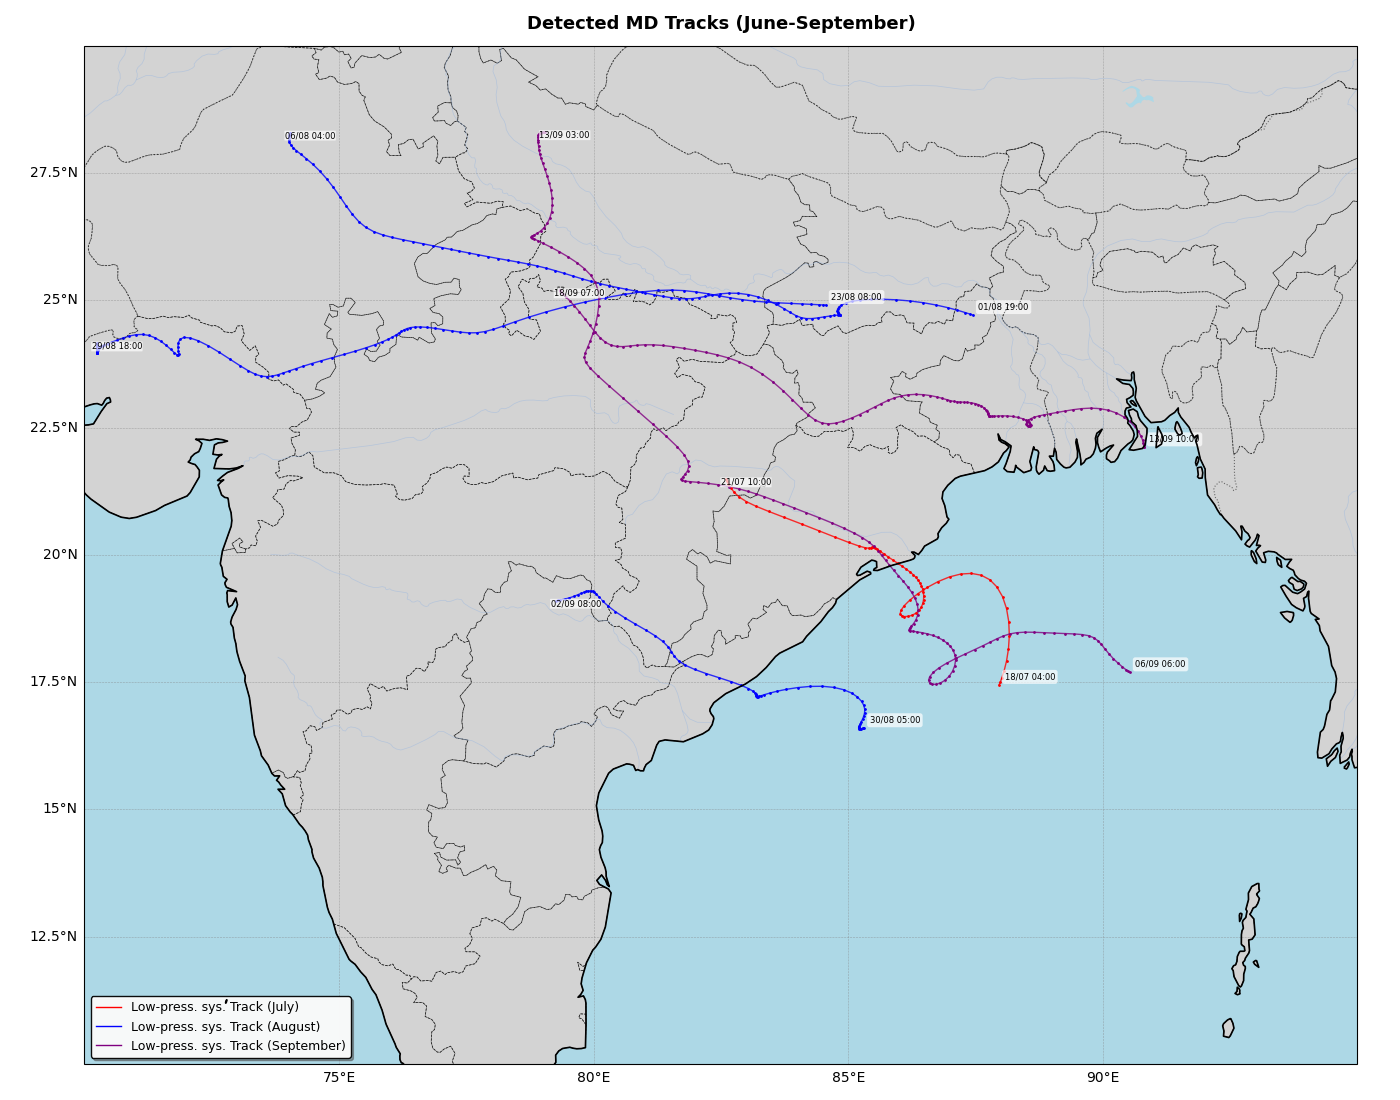
\includegraphics[width=1.01\linewidth]{images/MD-track.png}
			\textit{\footnotesize Detected MD tracks using ERA5 signle level Dataset}

			\column{0.5\textwidth}
			\vspace{0.3cm}
			\centering
			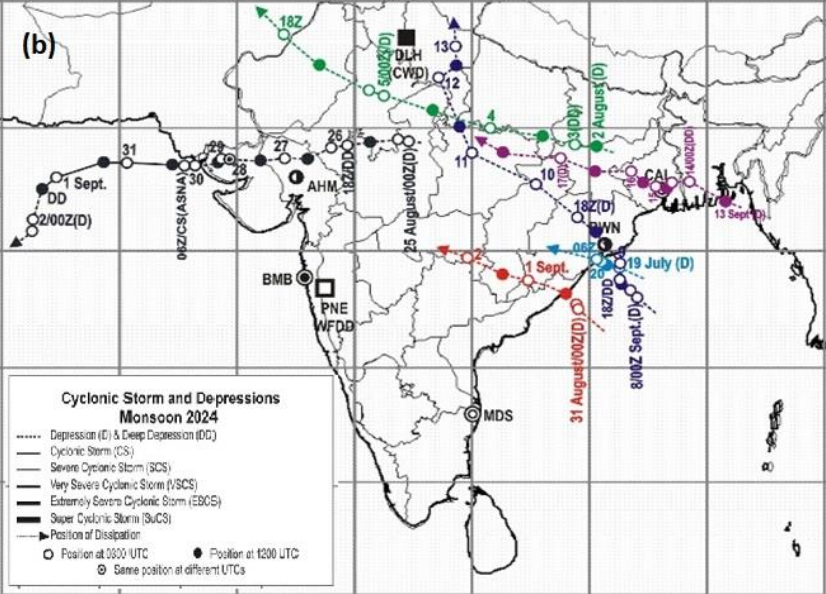
\includegraphics[width=1.02\linewidth]{images/IMD-report.png}
			\textit{\footnotesize IMD Monsoon Report 2024\footnotemark[1]}
		\end{columns}

		% \footnotetext[1]{\tiny Source: IMD Monsoon Report 2024, page 284, \href{https://mausam.imd.gov.in/responsive/monsooninformation.pdf}{\url{https://mausam.imd.gov.in/responsive/monsooninformation.php}}}
		\footnotetext[1]{\tiny Source: IMD Monsoon Report 2024, page 284, \url{https://mausam.imd.gov.in/responsive/monsooninformation.pdf}}

		% TODO:
		% \begin{block}{Key differences}
		% \end{block}
	\end{center}
\end{frame}

\begin{frame}{Comparison with IMD Report 2024}
	\begin{center}
		\begin{columns}[T]
			\column{0.5\textwidth}
			\textbf{Analysis using ERA5 single level dataset}
			% \footnotesize
			% \begin{columns}[T]
			% \column{0.45\textwidth}
			% \textbf{Detections:}
			%
			% \begin{tabular}{p{0.45\linewidth} p{0.35\linewidth}}
			% 	\toprule
			% 	Total Detections      & 6                  \\
			% 	\midrule
			% 	Originated over ocean & 3 (Tracks 1, 4, 5) \\
			% 	Originated over Land  & 3 (Tracks 2, 3, 6) \\
			% 	\bottomrule
			% \end{tabular}
			% \column{0.55\textwidth}

			\textbf{Monthly Distribution (2024):}
			\begin{tabular}{p{0.3\linewidth} p{0.35\linewidth}}
				\toprule
				Month      & No. of detections  \\
				\midrule
				June:      & 0                  \\
				July:      & 1 (Track 1)        \\
				August:    & 3 (Tracks 2, 3, 4) \\
				September: & 2 (Tracks 5, 6)    \\
				\bottomrule
				Total:     & 6
			\end{tabular}

			\column{0.5\textwidth}
			\vspace{0.3cm}
			\textbf{IMD Monsoon Report 2024:}
			\begin{tabular}{p{0.3\linewidth} p{0.35\linewidth}}
				\toprule
				Month           & No. of detections          \\
				\midrule
				June:           & 0                          \\
				July:           & 1                          \\
				August:         & 3                          \\
				September:      & 2                          \\
				\bottomrule
				Total reported: & 6 (D + DD)\footnotemark[2]
			\end{tabular}
		\end{columns}
	\end{center}

	\vspace{0.2cm}
	\begin{block}{Resolution}
		\small
		While the IMD report tracks systems at a \textbf{3-hour} interval, ERA5-based analysis uses a \textbf{1-hour temporal resolution}.
	\end{block}

	\footnotetext[2]{\tiny D = Depression and DD =Deep depressions}
\end{frame}

\begin{frame}{Overall Statistics \& Track Details}
	\begin{center}
		\begin{block}{Track Characteristics}
			\vspace{0.1cm}
			\centering
			\footnotesize
			\begin{tabular}{p{0.030\linewidth} p{0.086\linewidth} p{0.105\linewidth} p{0.132\linewidth} p{0.106\linewidth} p{0.104\linewidth} p{0.098\linewidth}}
				% \begin{tabular}{@{}clclllll@{}}
				\toprule
				                  & \multicolumn{4}{c}{\textbf{Detection using ERA5 data}} & \multicolumn{2}{c}{\textbf{IMD Monsoon Report 2024}}                                                                                                                                                   \\
				\cmidrule(lr){2-5} \cmidrule(lr){6-7}
				\textbf{Track ID} & \textbf{Origin}                                        & \textbf{Time (2024)}                                 & \textbf{Detected Duration} & \textbf{Category \tiny{($\geq$96h (4 days))}} & \textbf{IMD reported time (2024)} & \textbf{IMD reported duration} \\
				\midrule
				1                 & Over Ocean                                             & 18/07 04:00 - 21/07 07:00                            & 75h ($\sim$ 3 days)        & Short-lived                                   & 19/07 - 20/07                     & 3 days                         \\
				2                 & Over Land                                              & 01/08 19:00 - 06/08 04:00                            & 106h ($\sim$ 4.5 days)     & Long-lived                                    & 02/08 - 06/08                     & 4 days                         \\
				3                 & Over Land                                              & 23/08 08:00 - 29/08 10:00                            & 146h ($\sim$ 6 days)       & Long-lived                                    & 25/08 - 01/09                     & 8 days                         \\
				4                 & Over Ocean                                             & 30/08 05:00 - 02/09 08:00                            & 75h ($\sim$ 3 days)        & Short-lived                                   & 31/08 - 02/09                     & 3 days                         \\
				5                 & Over Ocean                                             & 06/09 06:00 - 13/09 03:00                            & 165h ($\sim$ 7 days)       & Long-lived                                    & 08/09 - 13/09                     & 5 days                         \\
				6                 & Over Land                                              & 13/09 12:00 - 18/09 07:00                            & 117h ($\sim$ 5 days)       & Long-lived                                    & 13/09 - 18/09                     & 5 days                         \\
				\bottomrule
			\end{tabular}
		\end{block}

		\tiny
		\textit{Mean Detection Duration for all tracks is $115.2 \pm 38.3$ hours.}

		\footnotetext[2]{\tiny Short or long lived MDs are Categorized based on their duration less or more than $96$ hours ($\sim 4$ days)}
	\end{center}
\end{frame}

% %%%%%%%%%%%%%%%% Track 1 %%%%%%%%%%%%%%
\begin{frame}{Track 1 Details}
	\begin{center}
		\begin{columns}[T]
			\column{0.6\textwidth}
			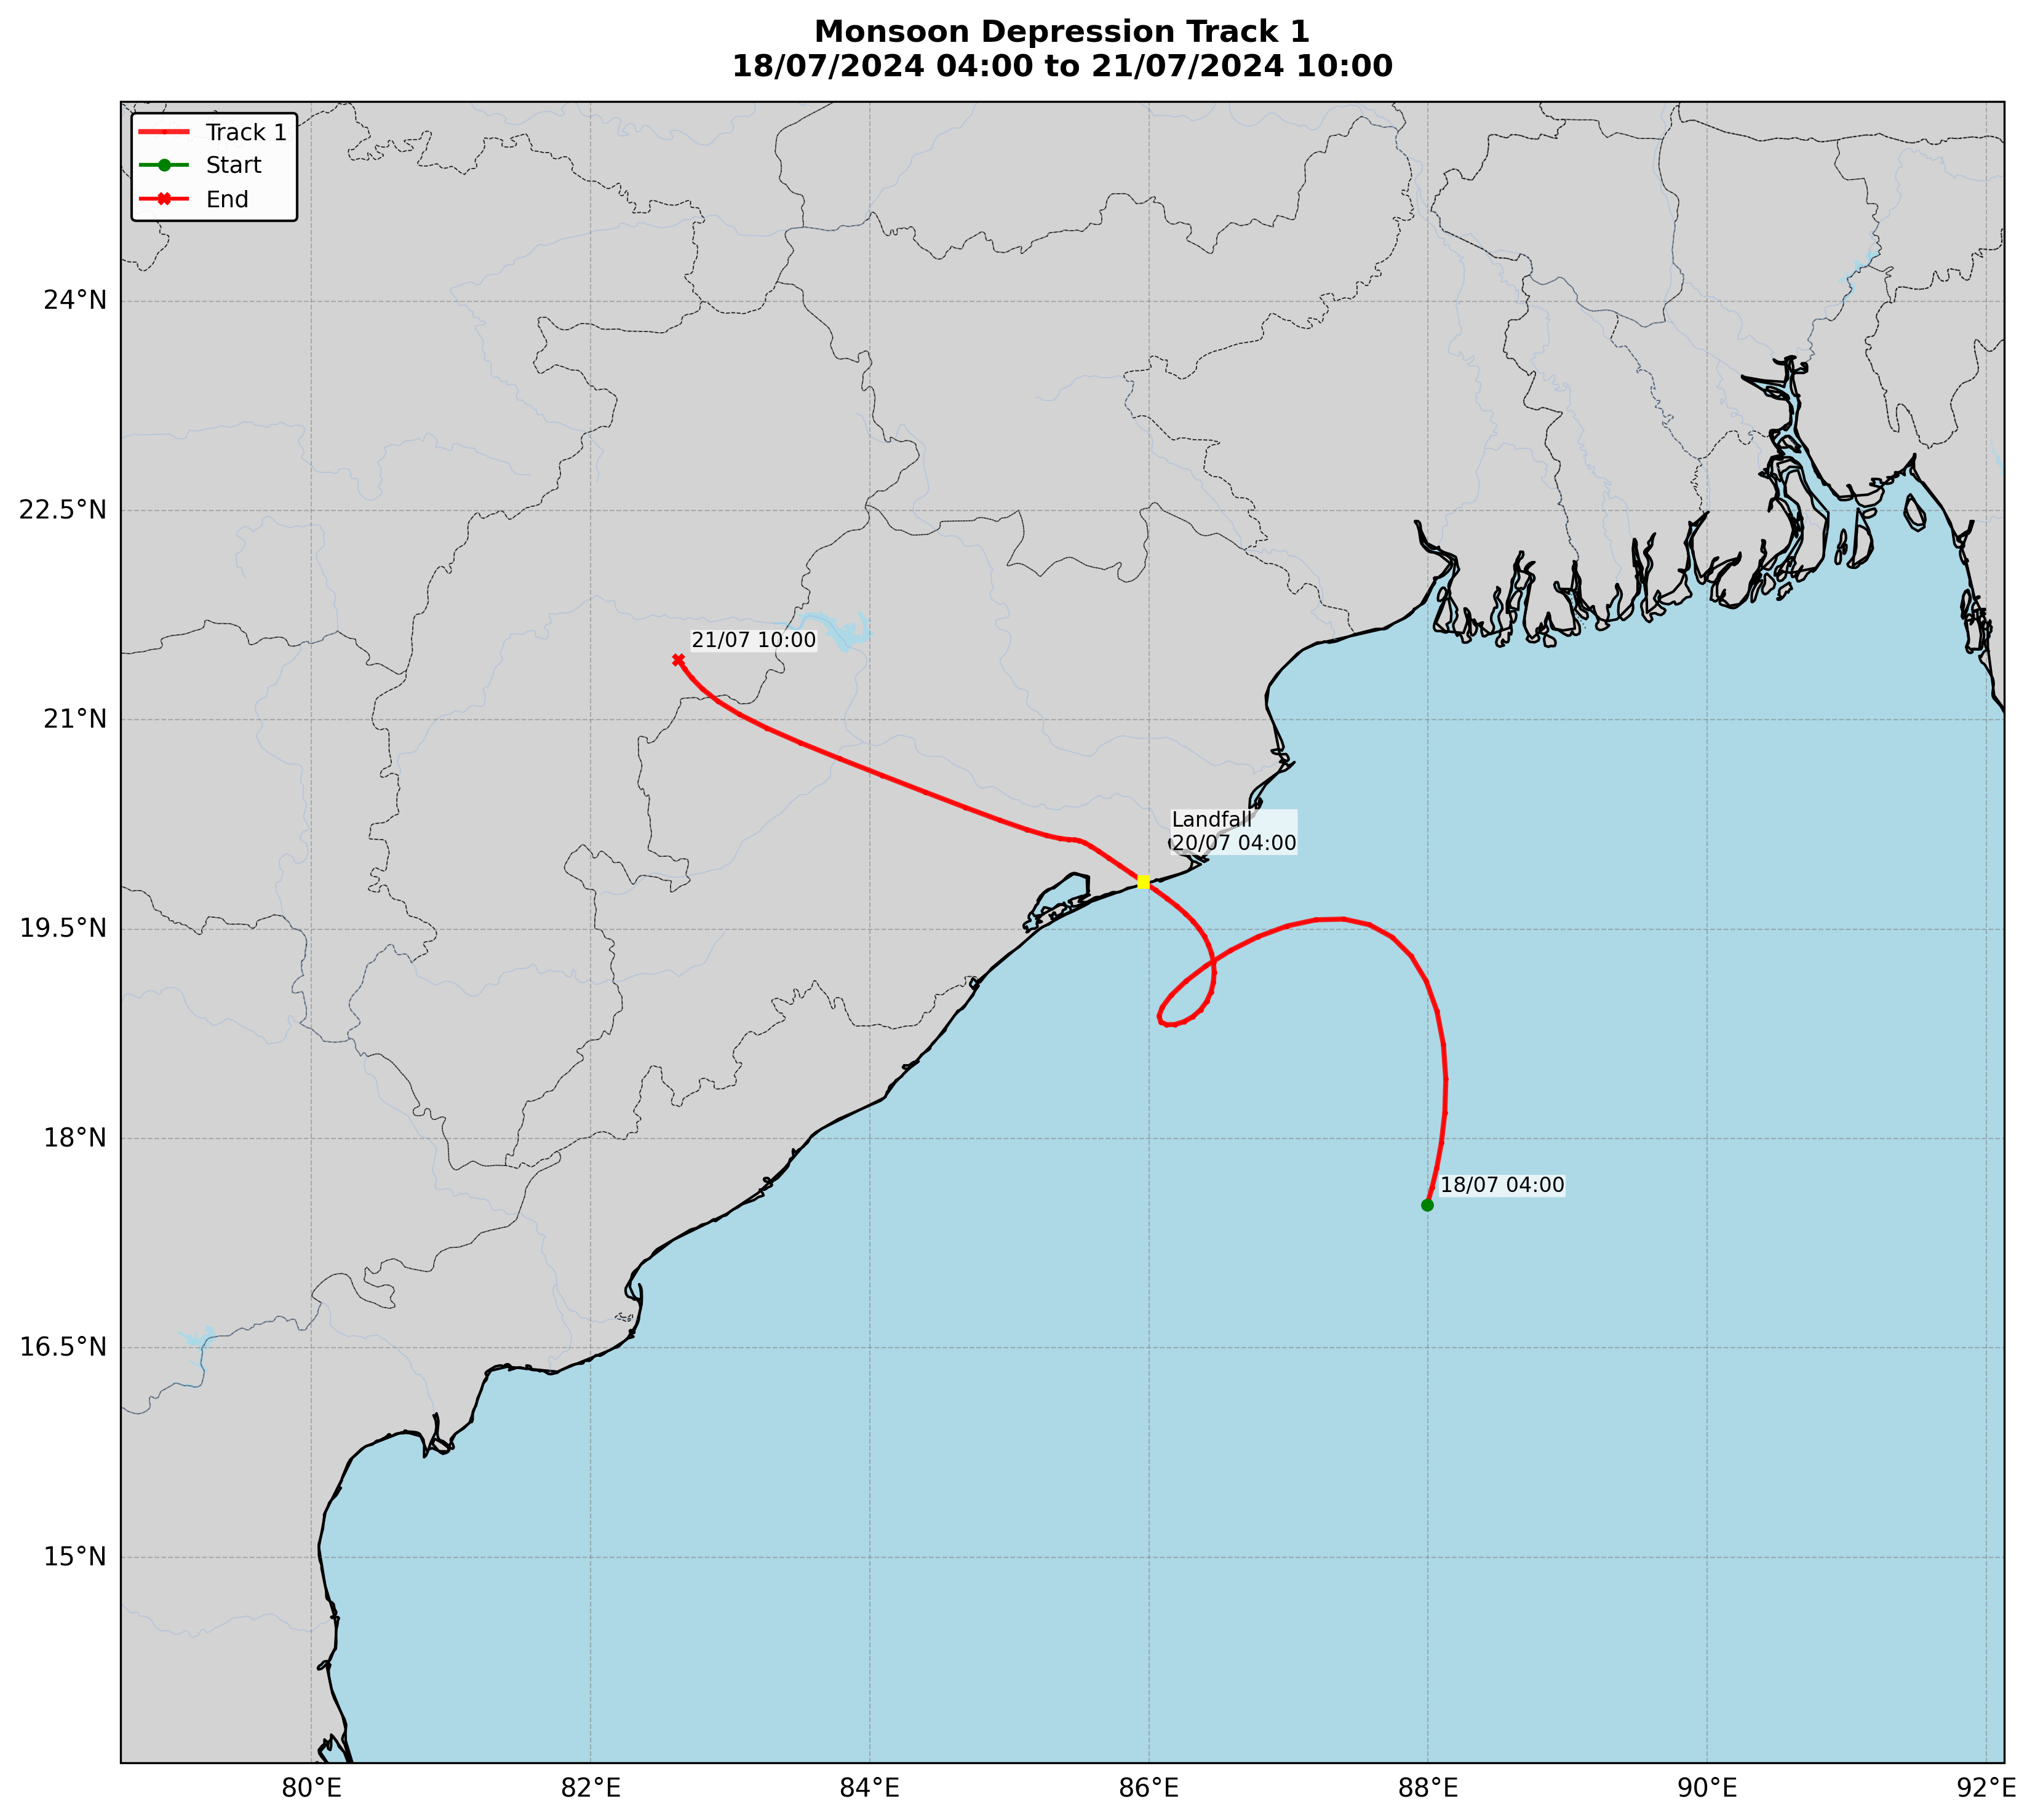
\includegraphics[width=0.95\textwidth]{../version5-with-no-ocean-masking/output/track_1/MD-track-1-detailed.png}

			\column{0.4\textwidth}
			\begin{block}{Statistics}
				\begin{itemize}
					\item Duration: 75 hours ($\sim$ 3 days)
					\item Category: short-lived MD
					\item Originated: over ocean
				\end{itemize}
			\end{block}
		\end{columns}
	\end{center}
\end{frame}

% 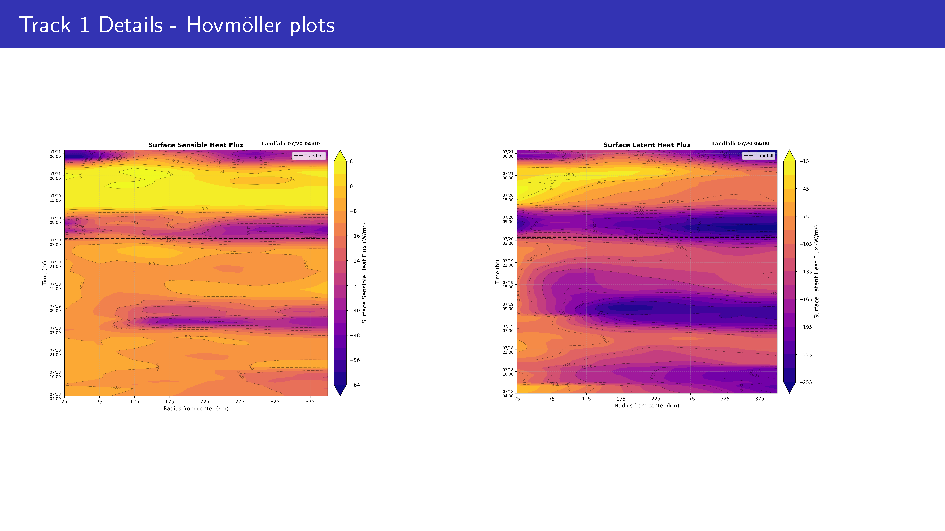
\includepdf[
% 	pages=-,
% 	scale=1,
% 	frame=true,
% 	pagecommand={\thispagestyle{empty}},  % Remove page numbers
% 	offset=0mm 0mm,       % Adjust position
% 	% templatesize={\textwidth}{\textheight} % Match template size
% ]{hovmoller-slides/hov-1.pdf}

% \begin{frame}{Track 1 Details - Precipitation and soil moisture over time along track}
% 	\begin{center}
% 		\includegraphics[width=0.8\textwidth]{../version5-with-no-ocean-masking/output/track_1/correlation_analysis/time_series/track_1_time_series.png}
% 	\end{center}
% \end{frame}

\begin{frame}{Track 1 Details - Translation speed of MD}
	\begin{center}
		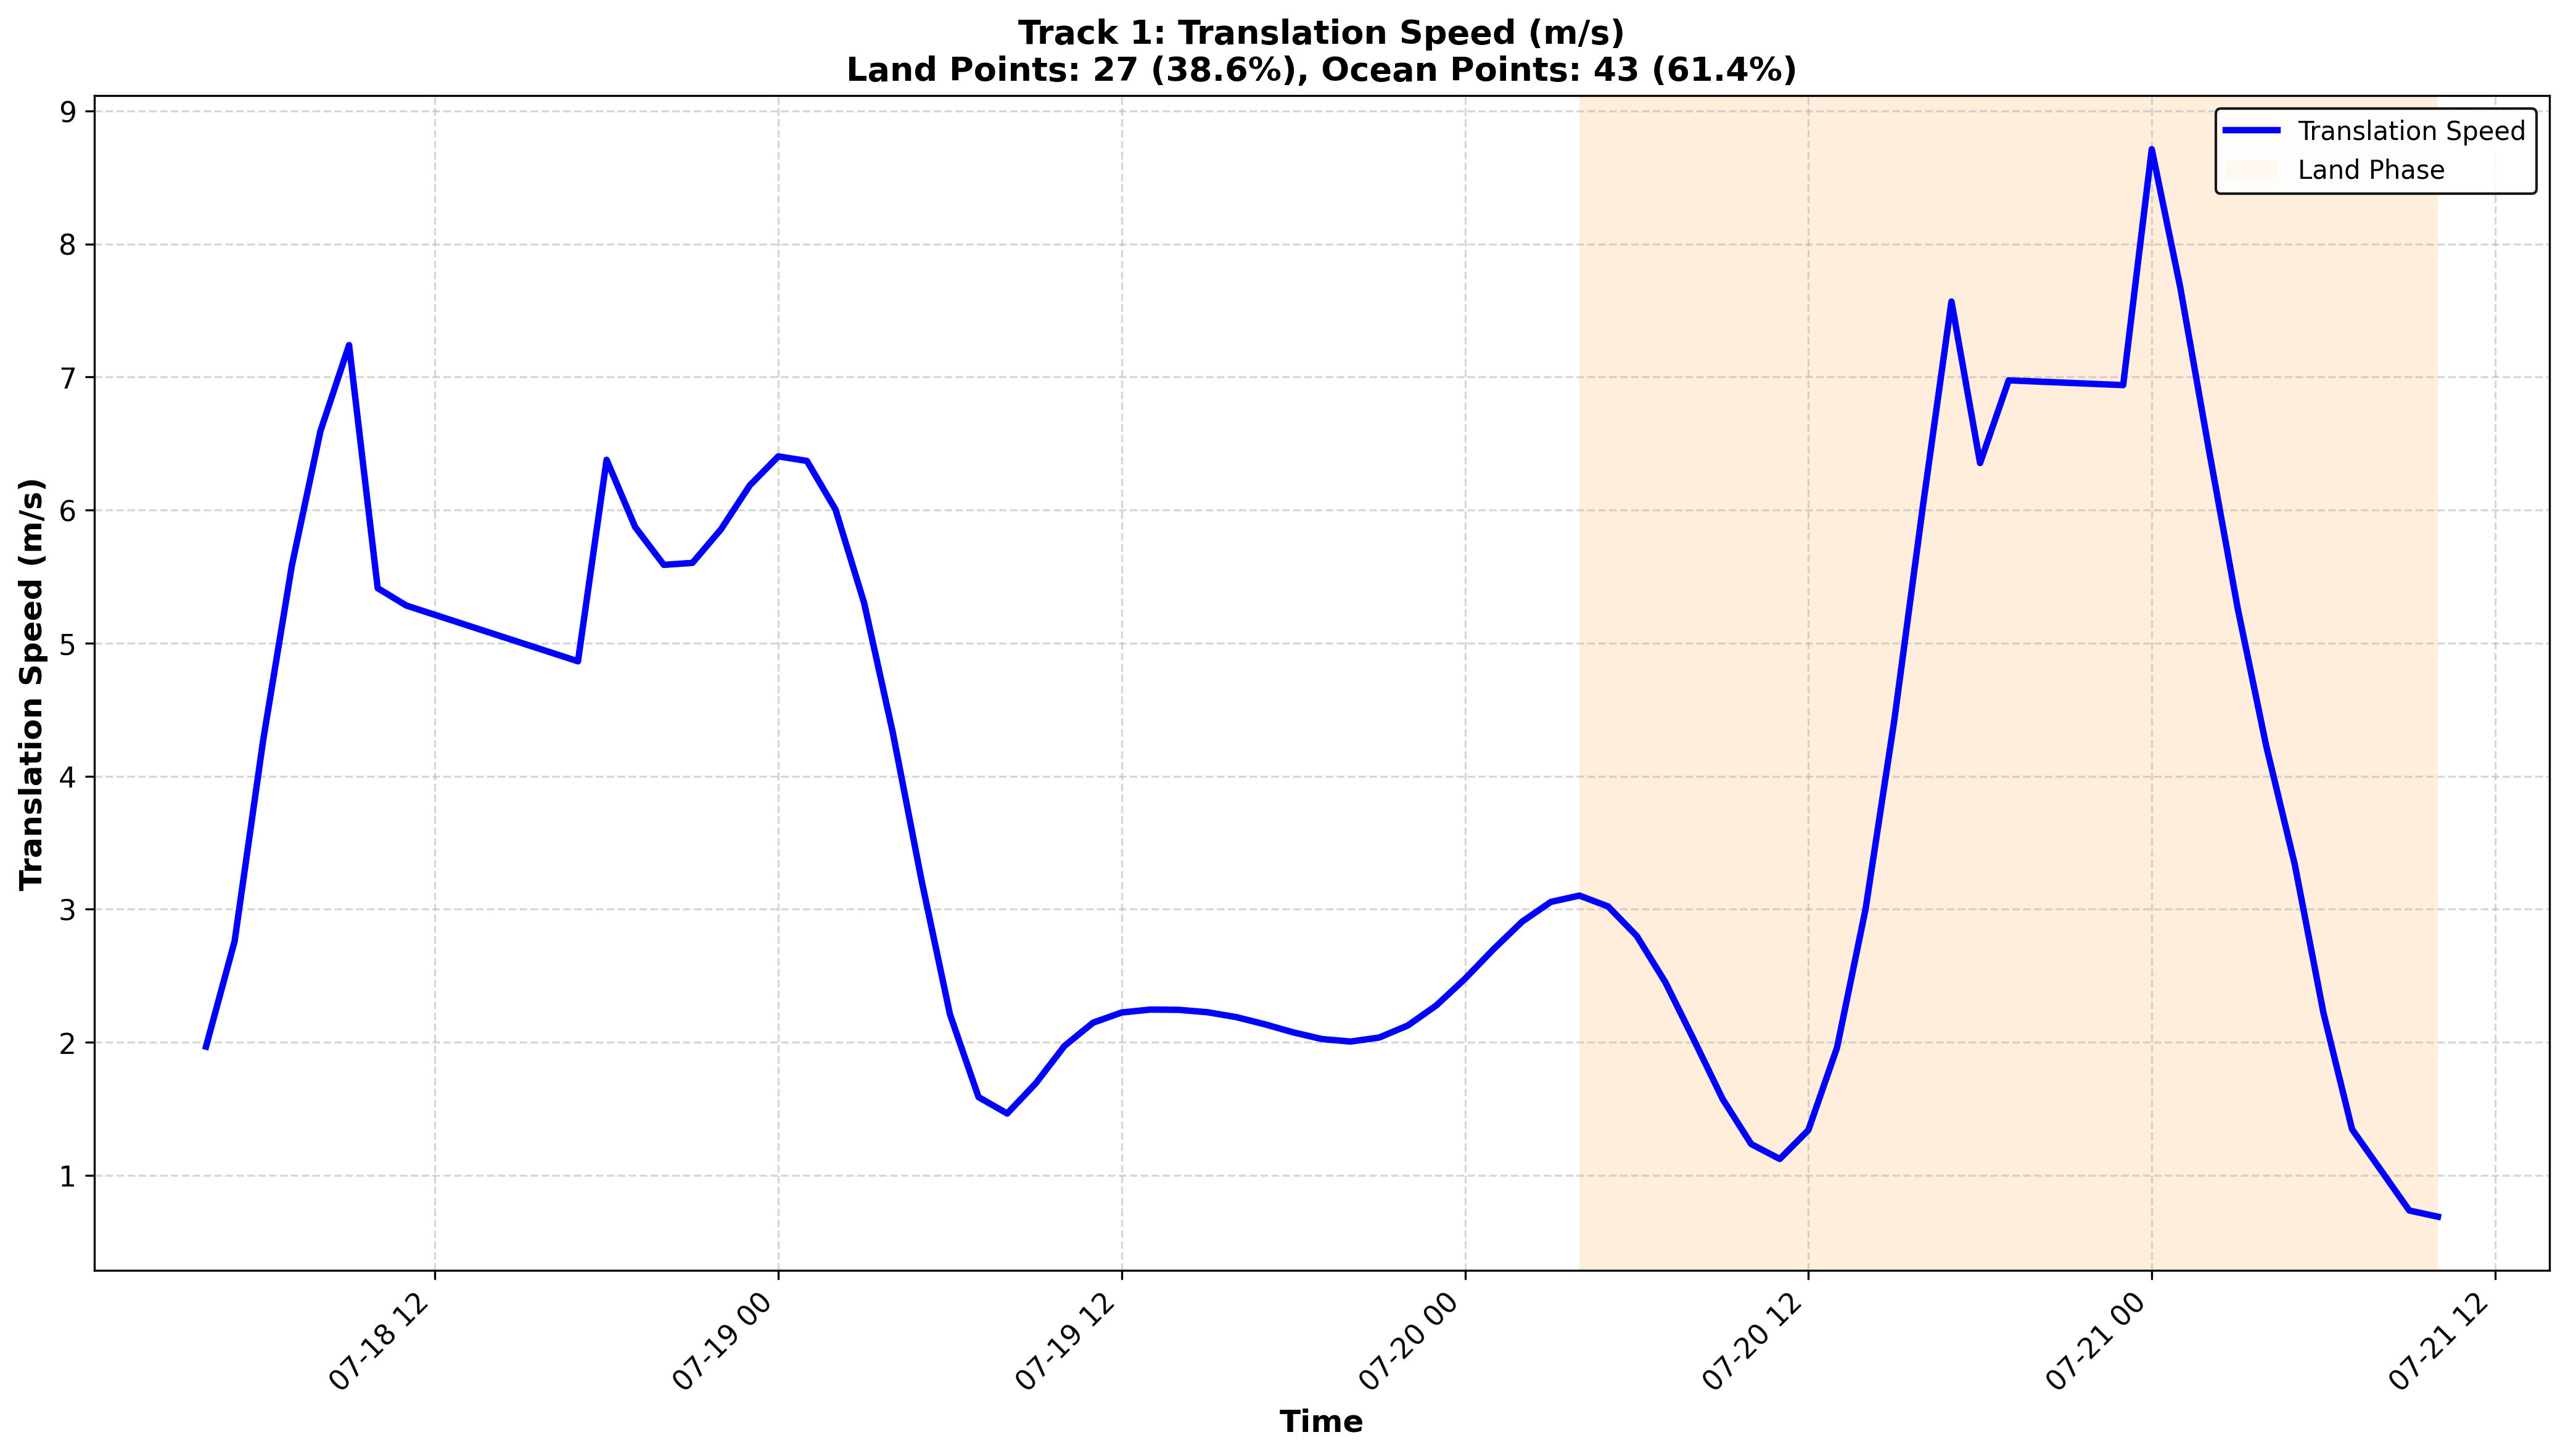
\includegraphics[width=0.8\textwidth]{../version5-with-no-ocean-masking/output/track_1/translational-speed/track_1_speed_ms.png}
	\end{center}
\end{frame}

\begin{frame}{Track 1 Details - Lag Correlation}
	\begin{center}
		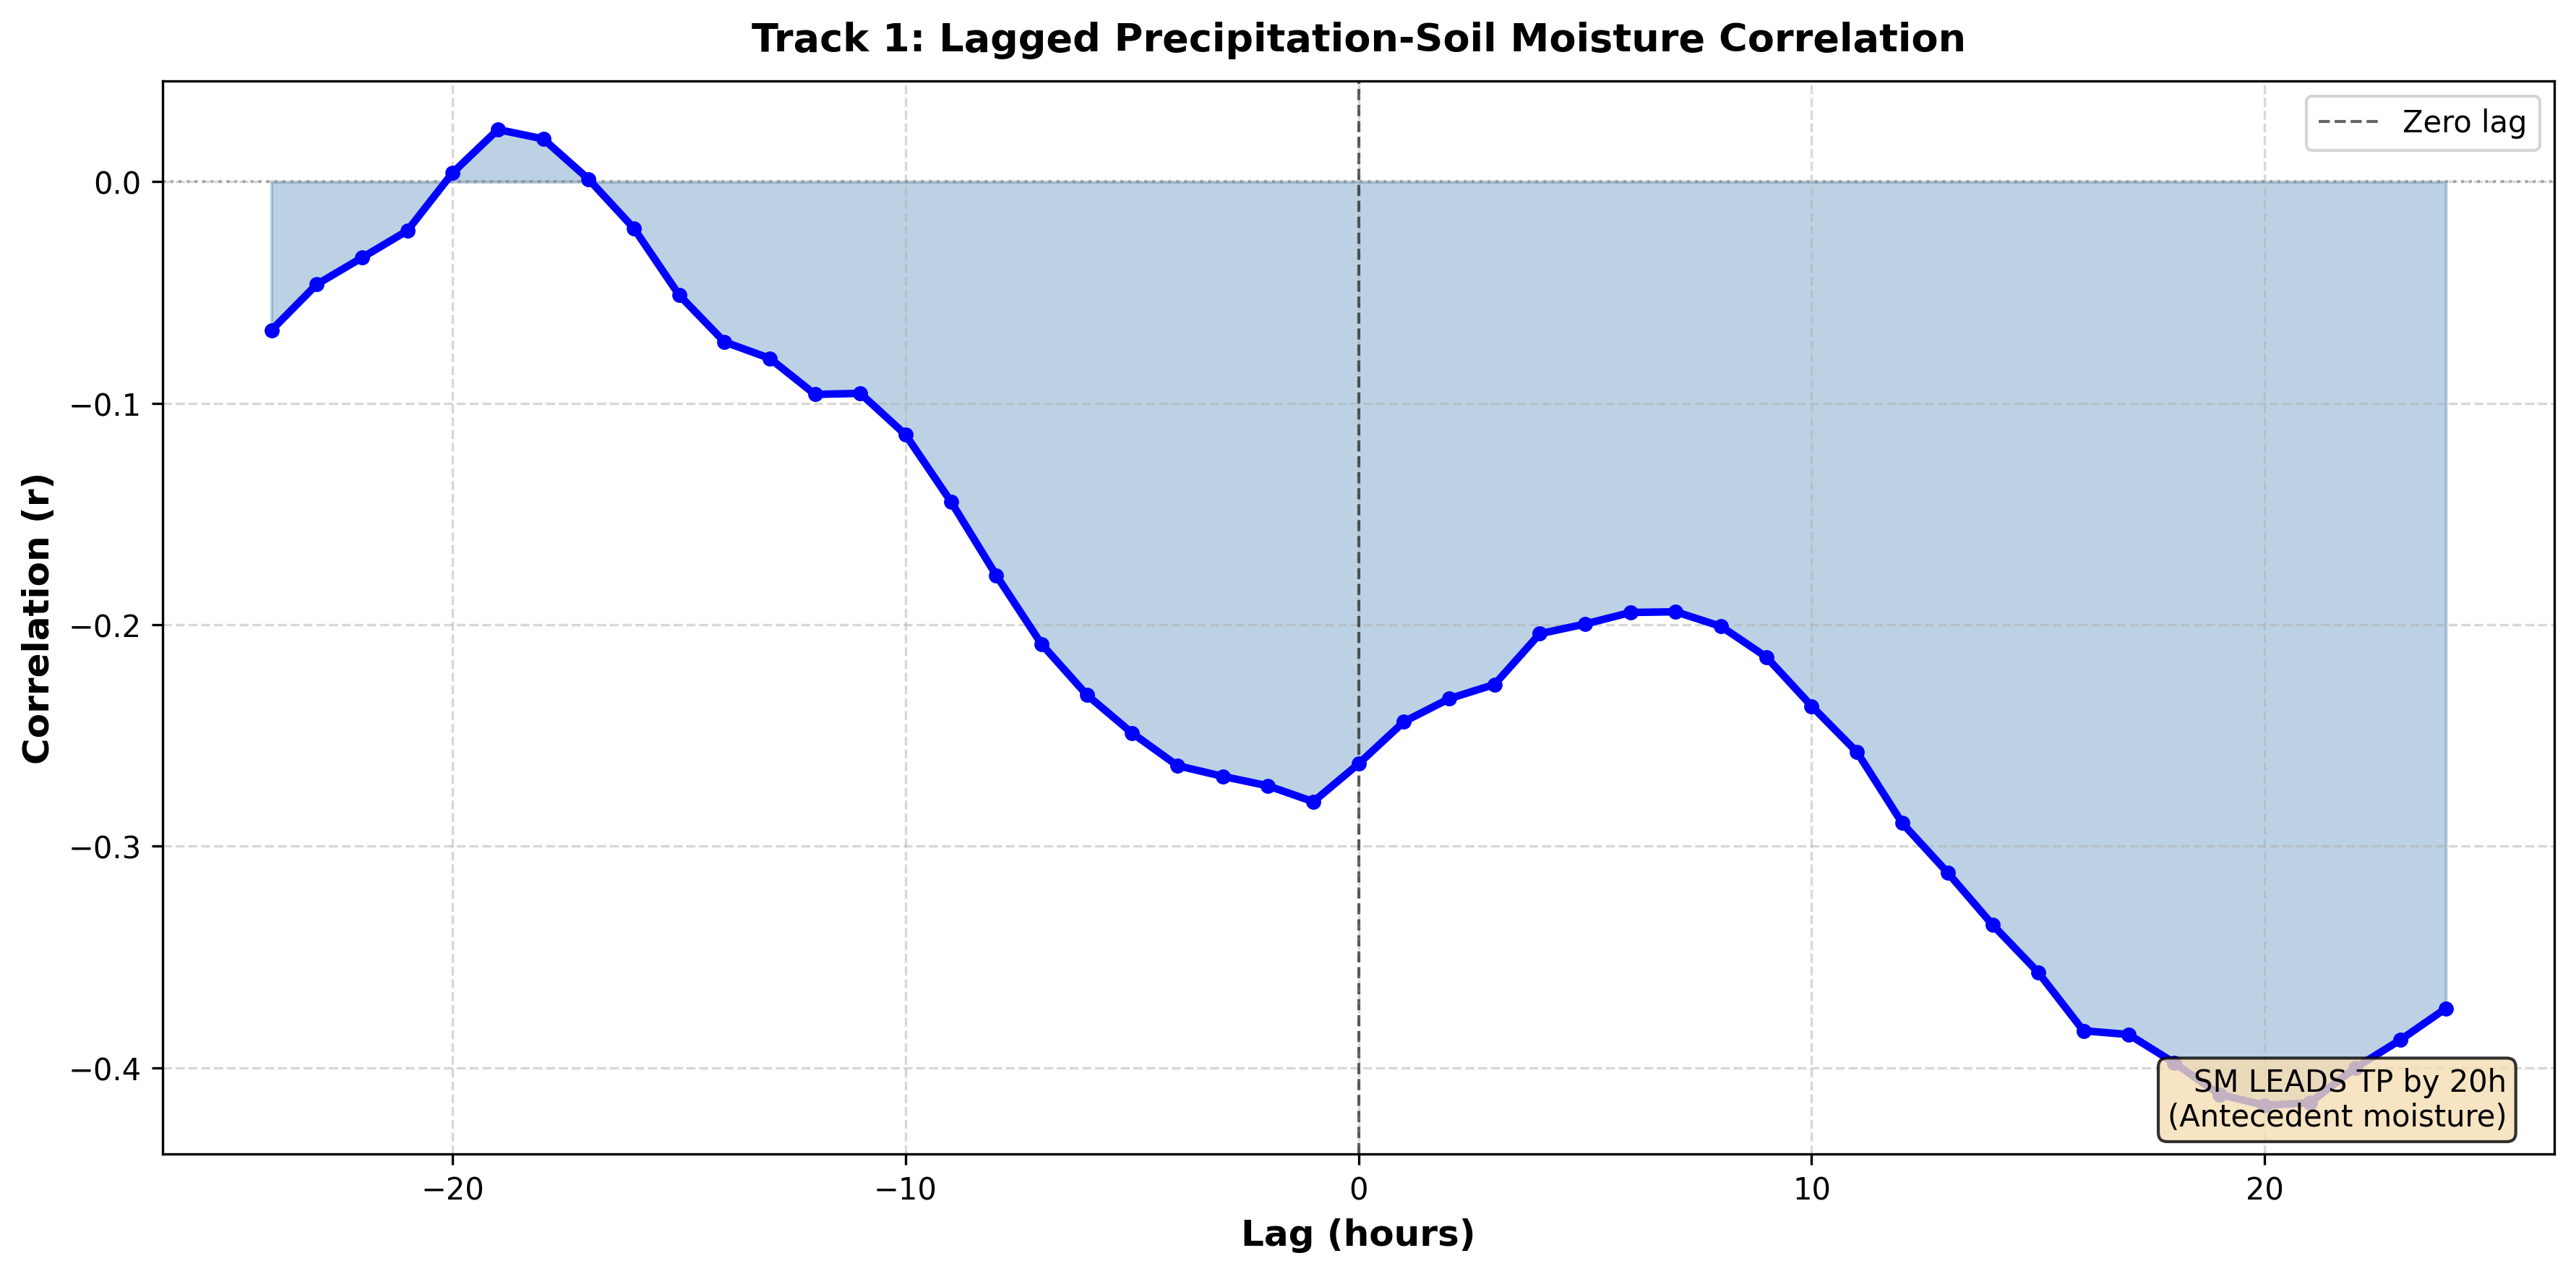
\includegraphics[width=0.8\textwidth]{../version5-with-no-ocean-masking/output/track_1/correlation_analysis/lag_correlation/track_1_lag_corr.png}
	\end{center}
\end{frame}

\begin{frame}{Track 1 Details - TP - SWVL1 Correlation}
	\begin{center}
		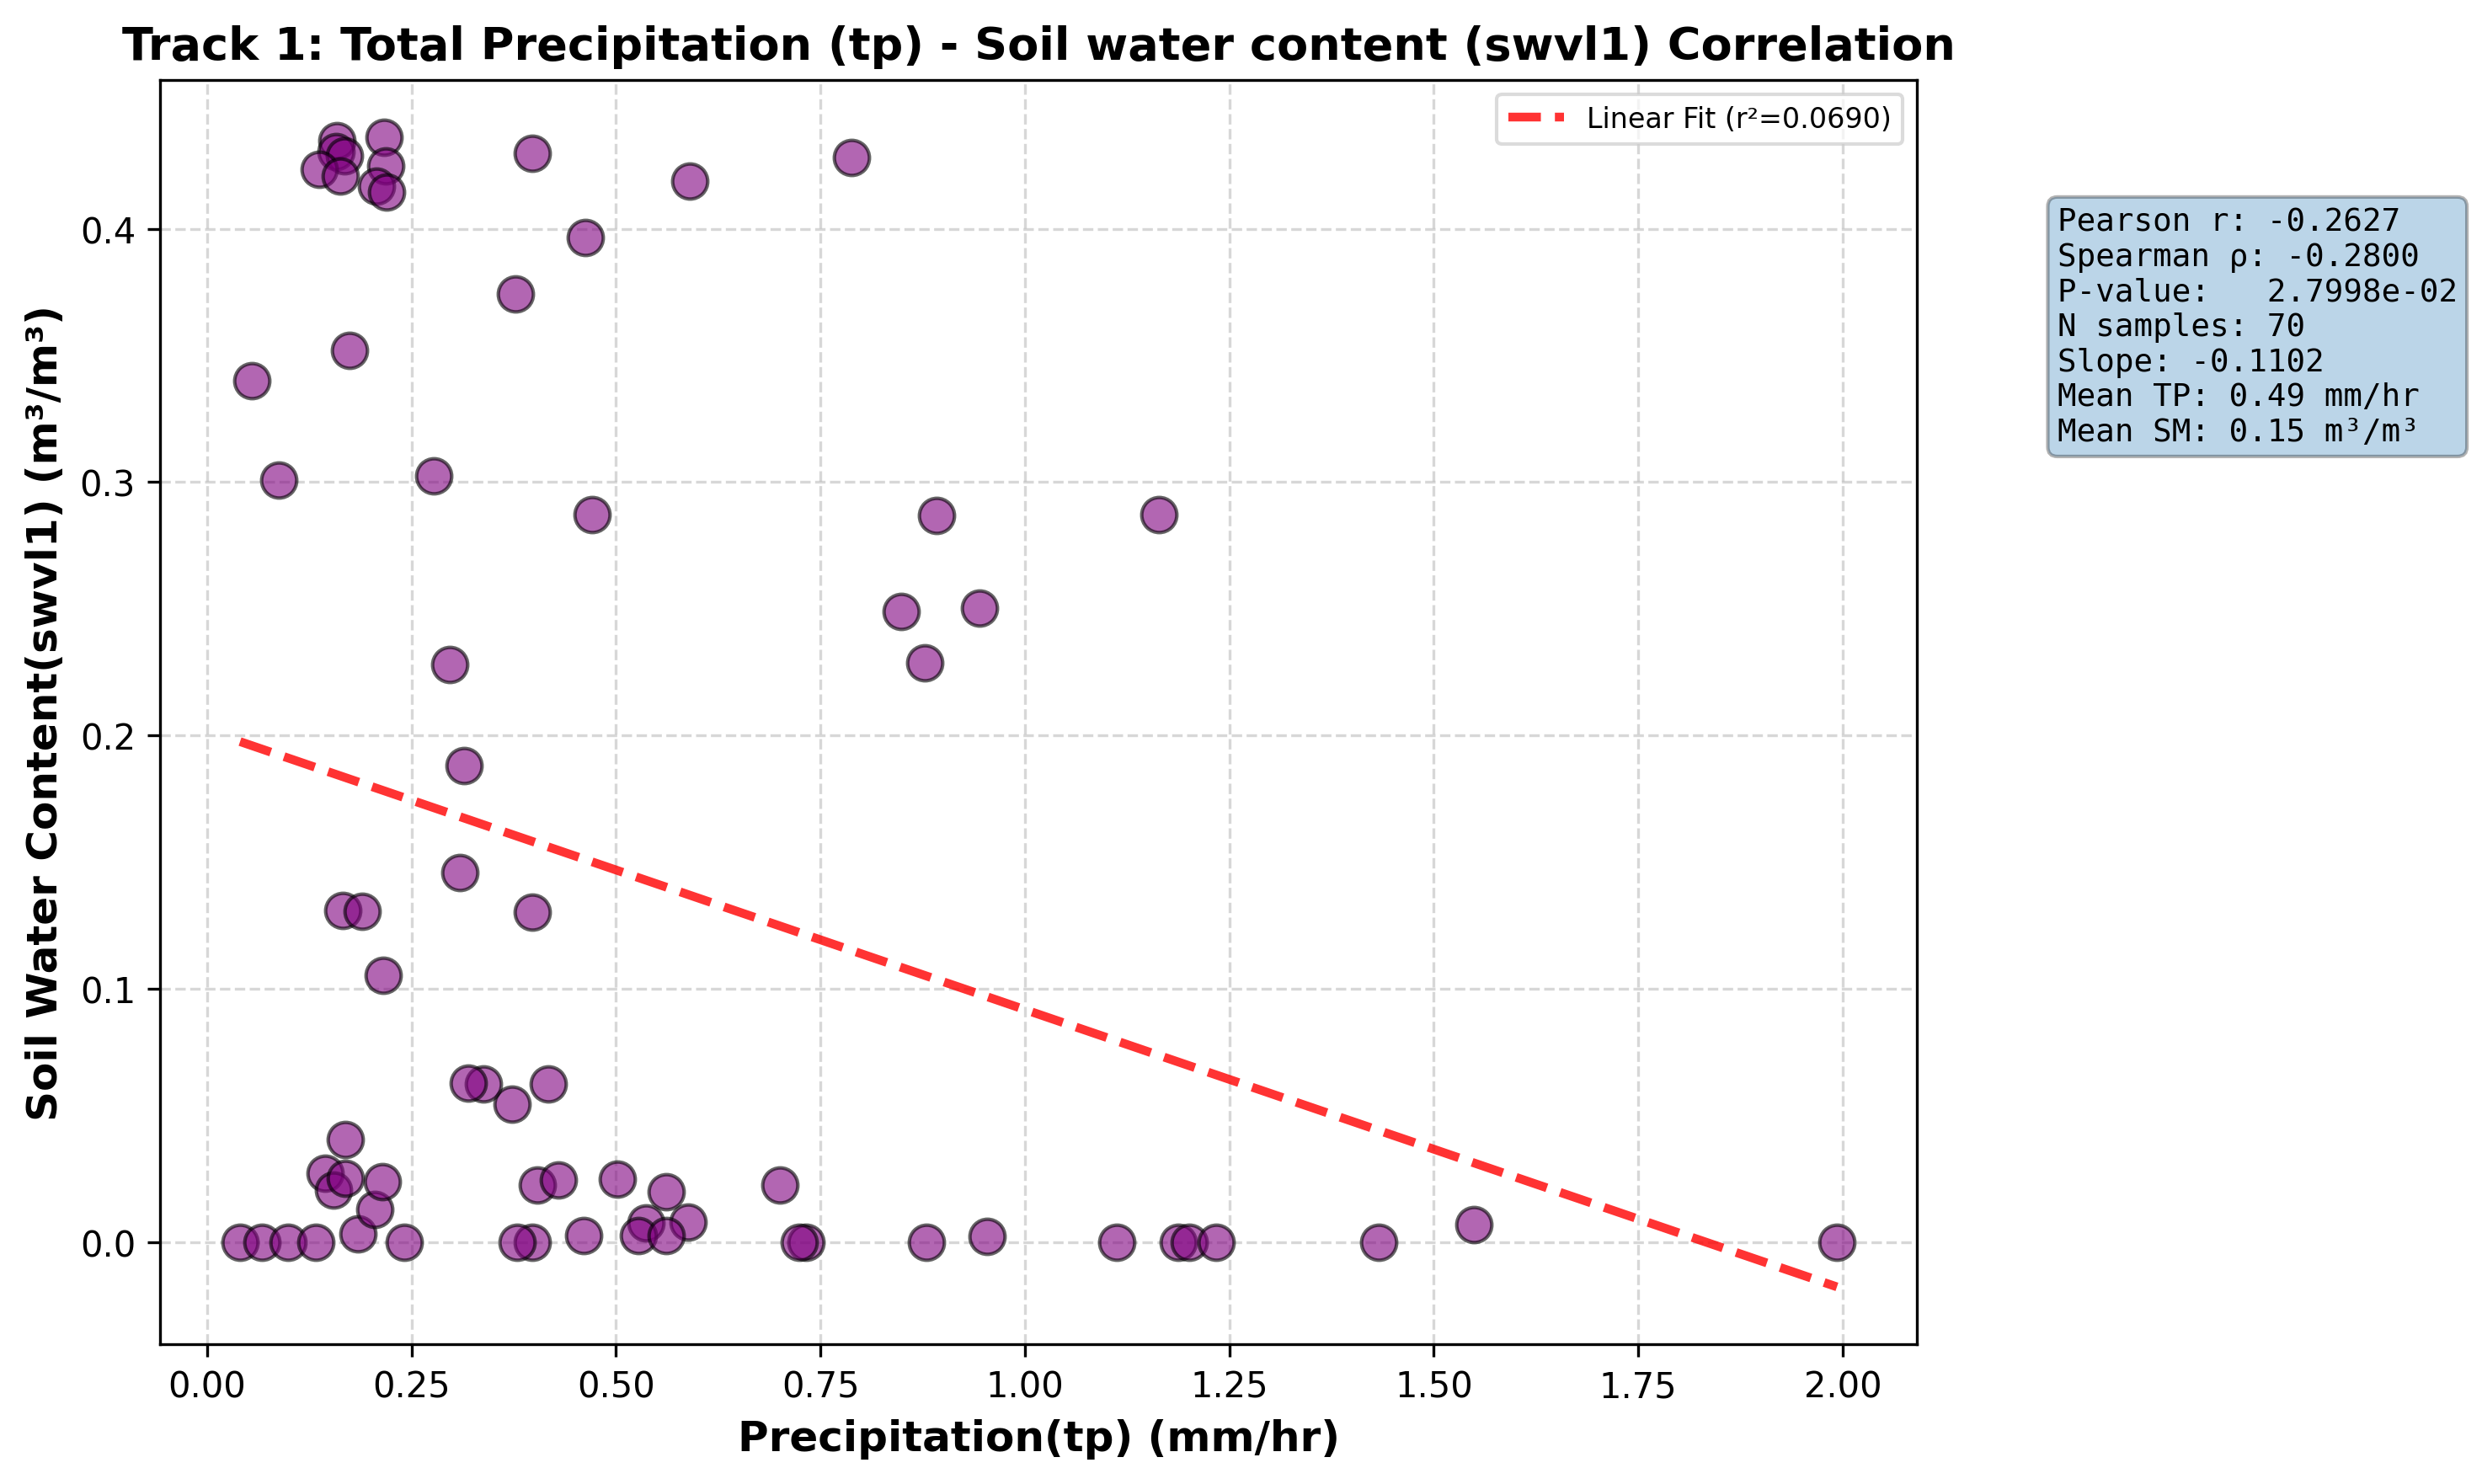
\includegraphics[width=0.7\textwidth]{../version5-with-no-ocean-masking/output/track_1/correlation_analysis/scatter_plots/track_1_scatter.png}
	\end{center}
\end{frame}

\begin{frame}{Track 1 Details - Spatial distribution of TP and SWVL1}
	\begin{center}
		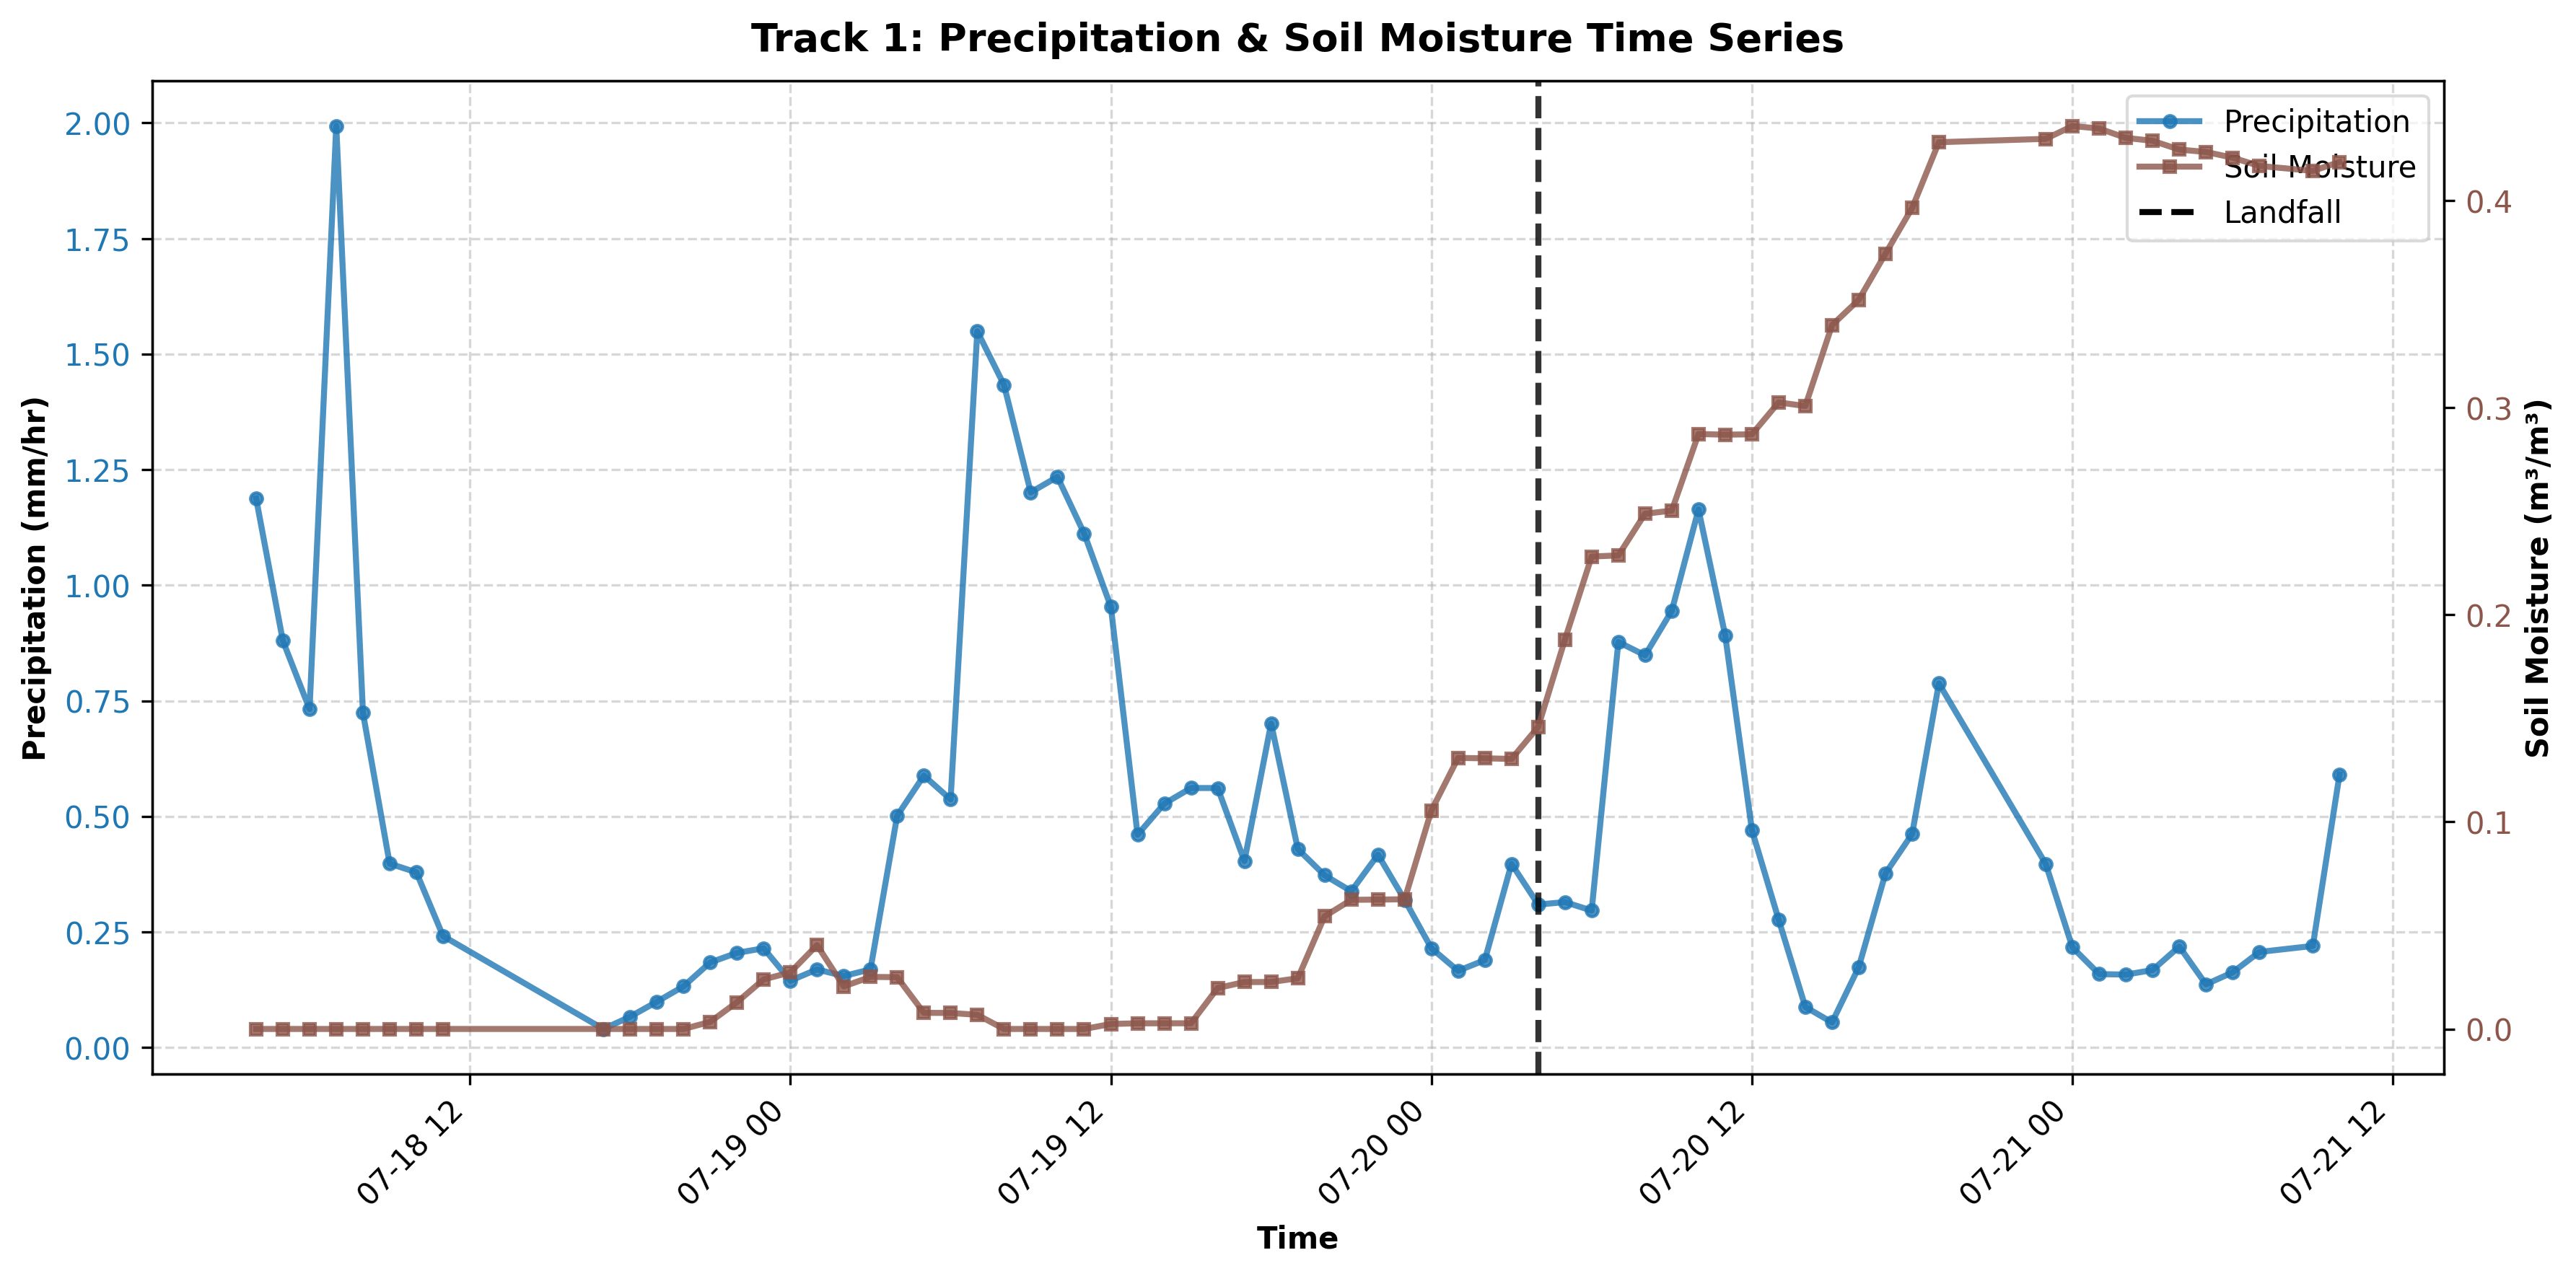
\includegraphics[width=0.7\textwidth]{../version5-with-no-ocean-masking/output/track_1/correlation_analysis/time_series/track_1_tp_sm_time_series.png}
	\end{center}
\end{frame}

% \begin{frame}{Track 1 Details - Heat fluxes transition}
% 	\begin{center}
% 		\includegraphics[width=0.8\textwidth]{../version5-with-no-ocean-masking/output/track_1/flux_analysis/track_1_analysis/track_1_heat_fluxes_trasnsition.png}
% 	\end{center}
% \end{frame}

\begin{frame}{Track 1 Details - Heat flux analysis}
	\begin{center}
		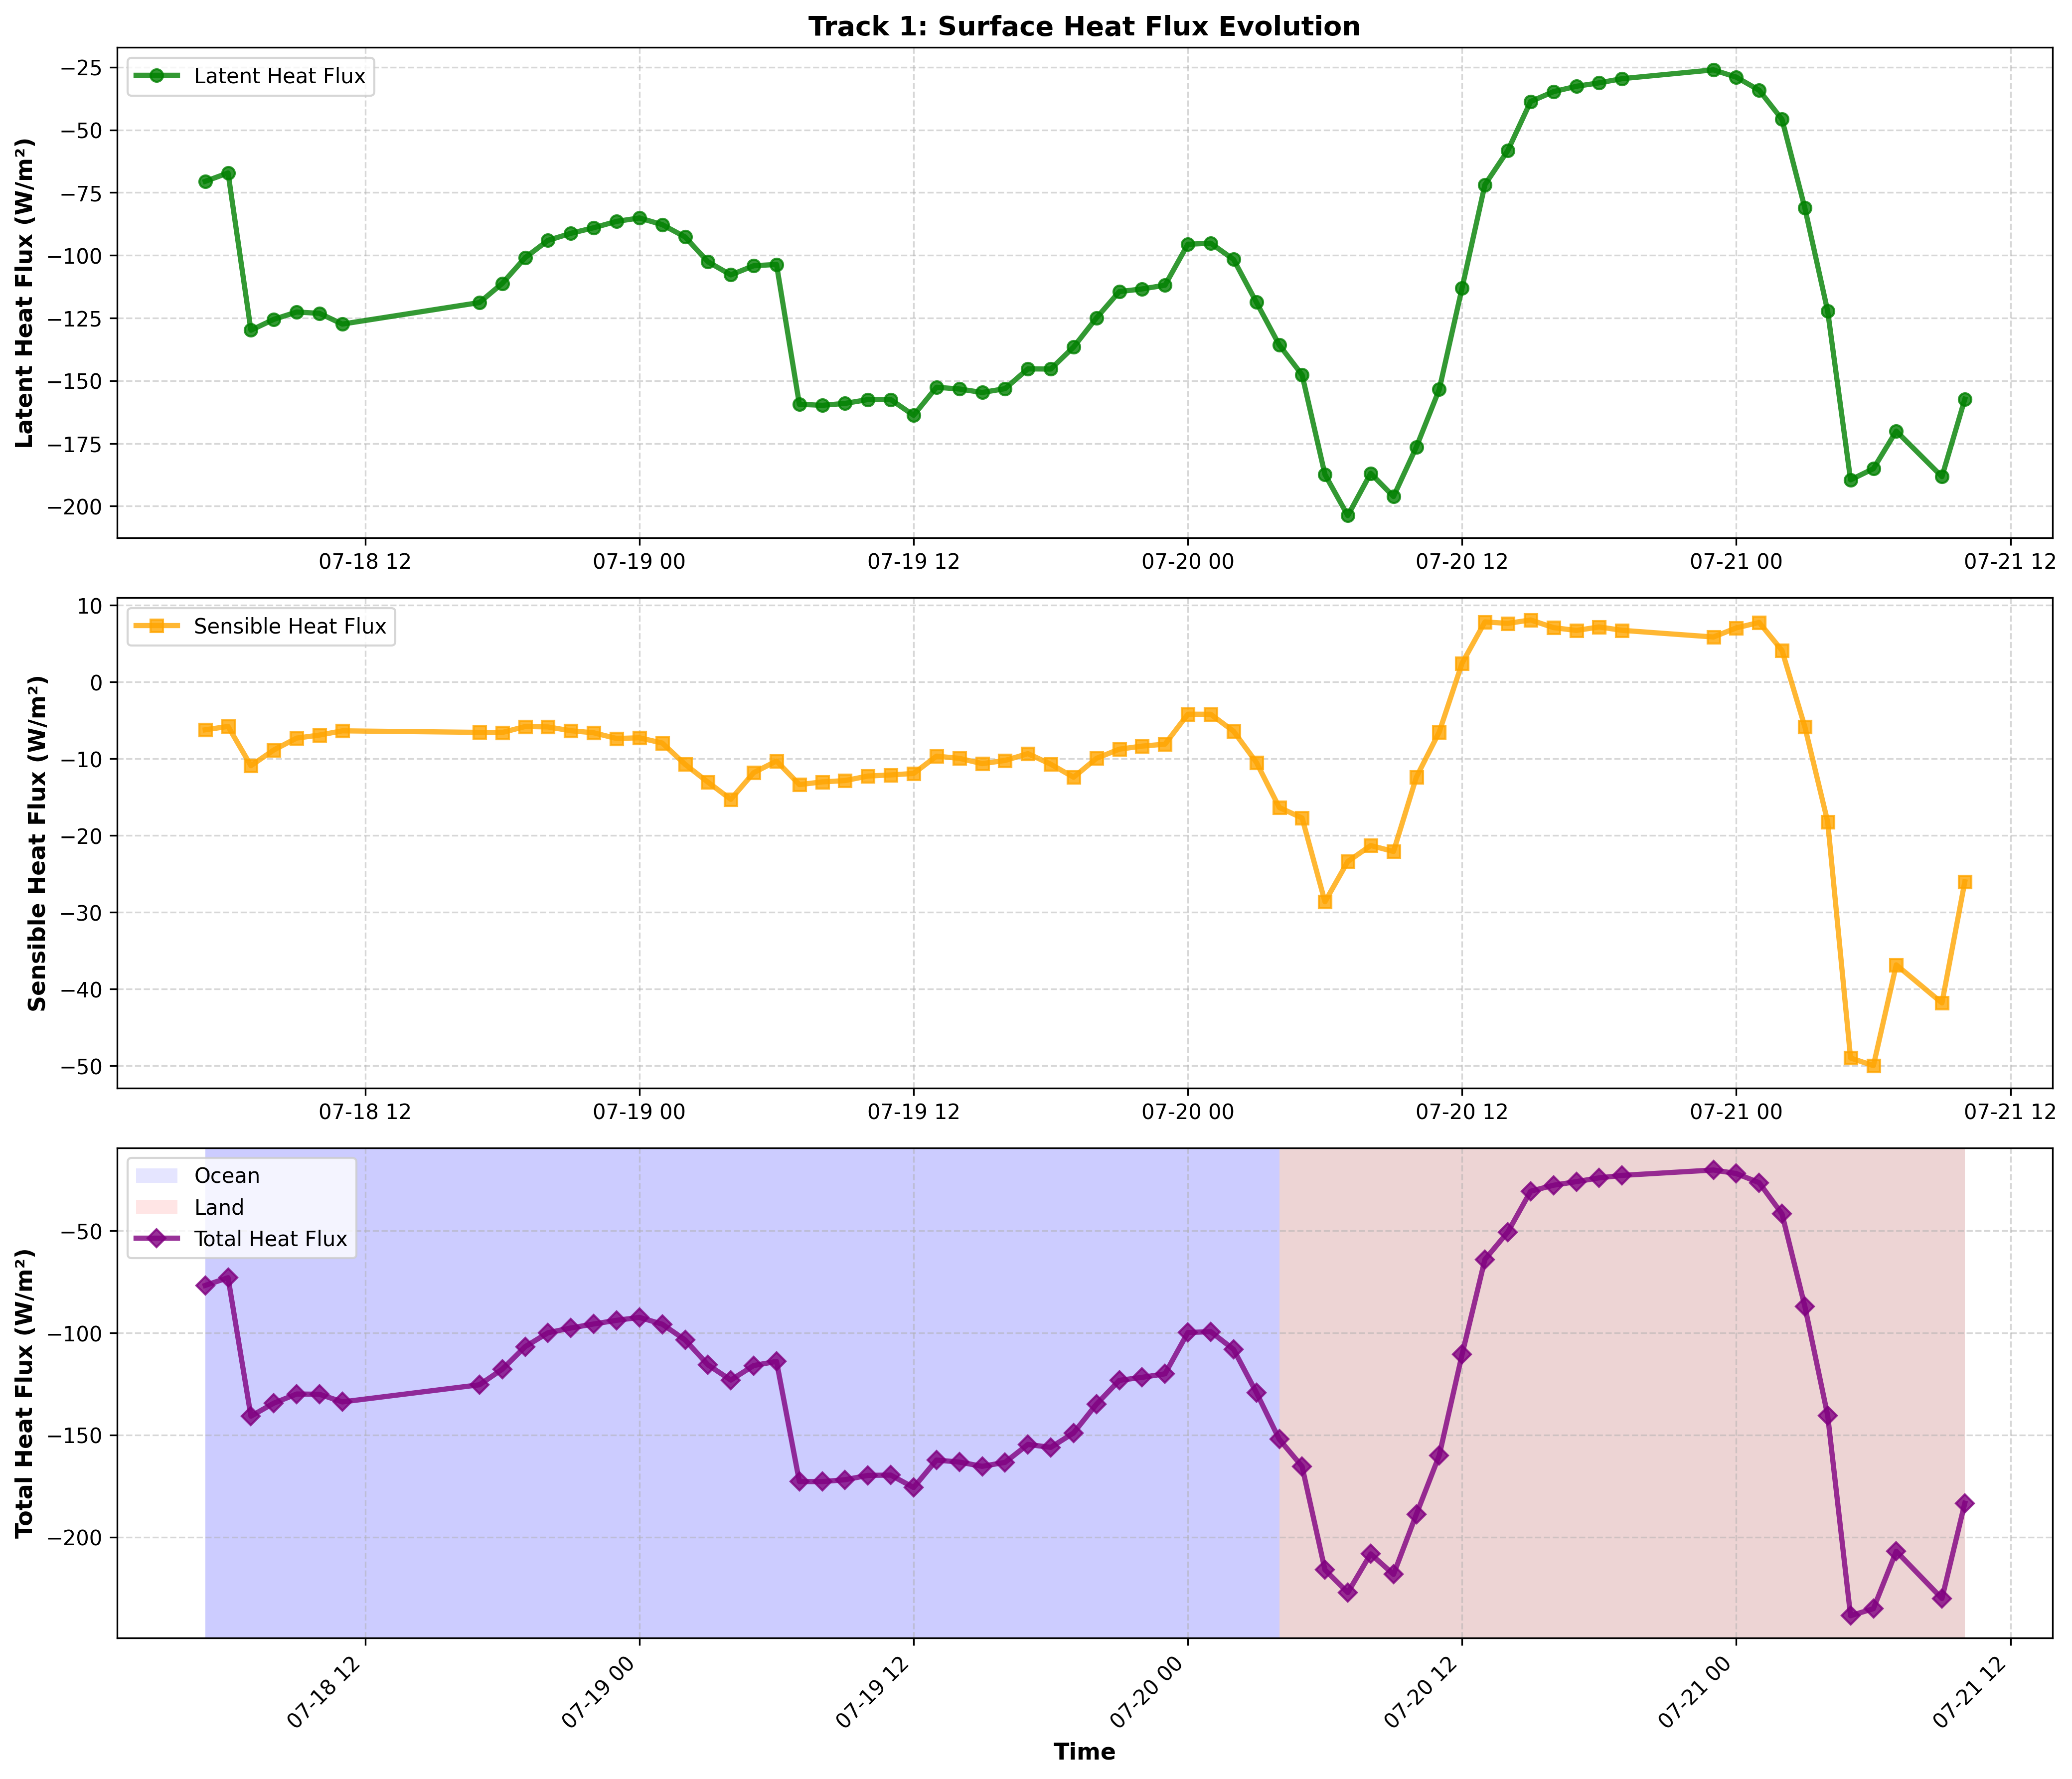
\includegraphics[width=0.6\textwidth]{../version5-with-no-ocean-masking/output/track_1/heat_flux_analysis/track_1_heat_flux_timeseries.png}
	\end{center}
\end{frame}

% % %%%%%%%%%%%%%%%% Track 2 %%%%%%%%%%%%%%
\begin{frame}{Track 2 Details}
	\begin{center}
		\begin{columns}[T]
			\column{0.6\textwidth}
			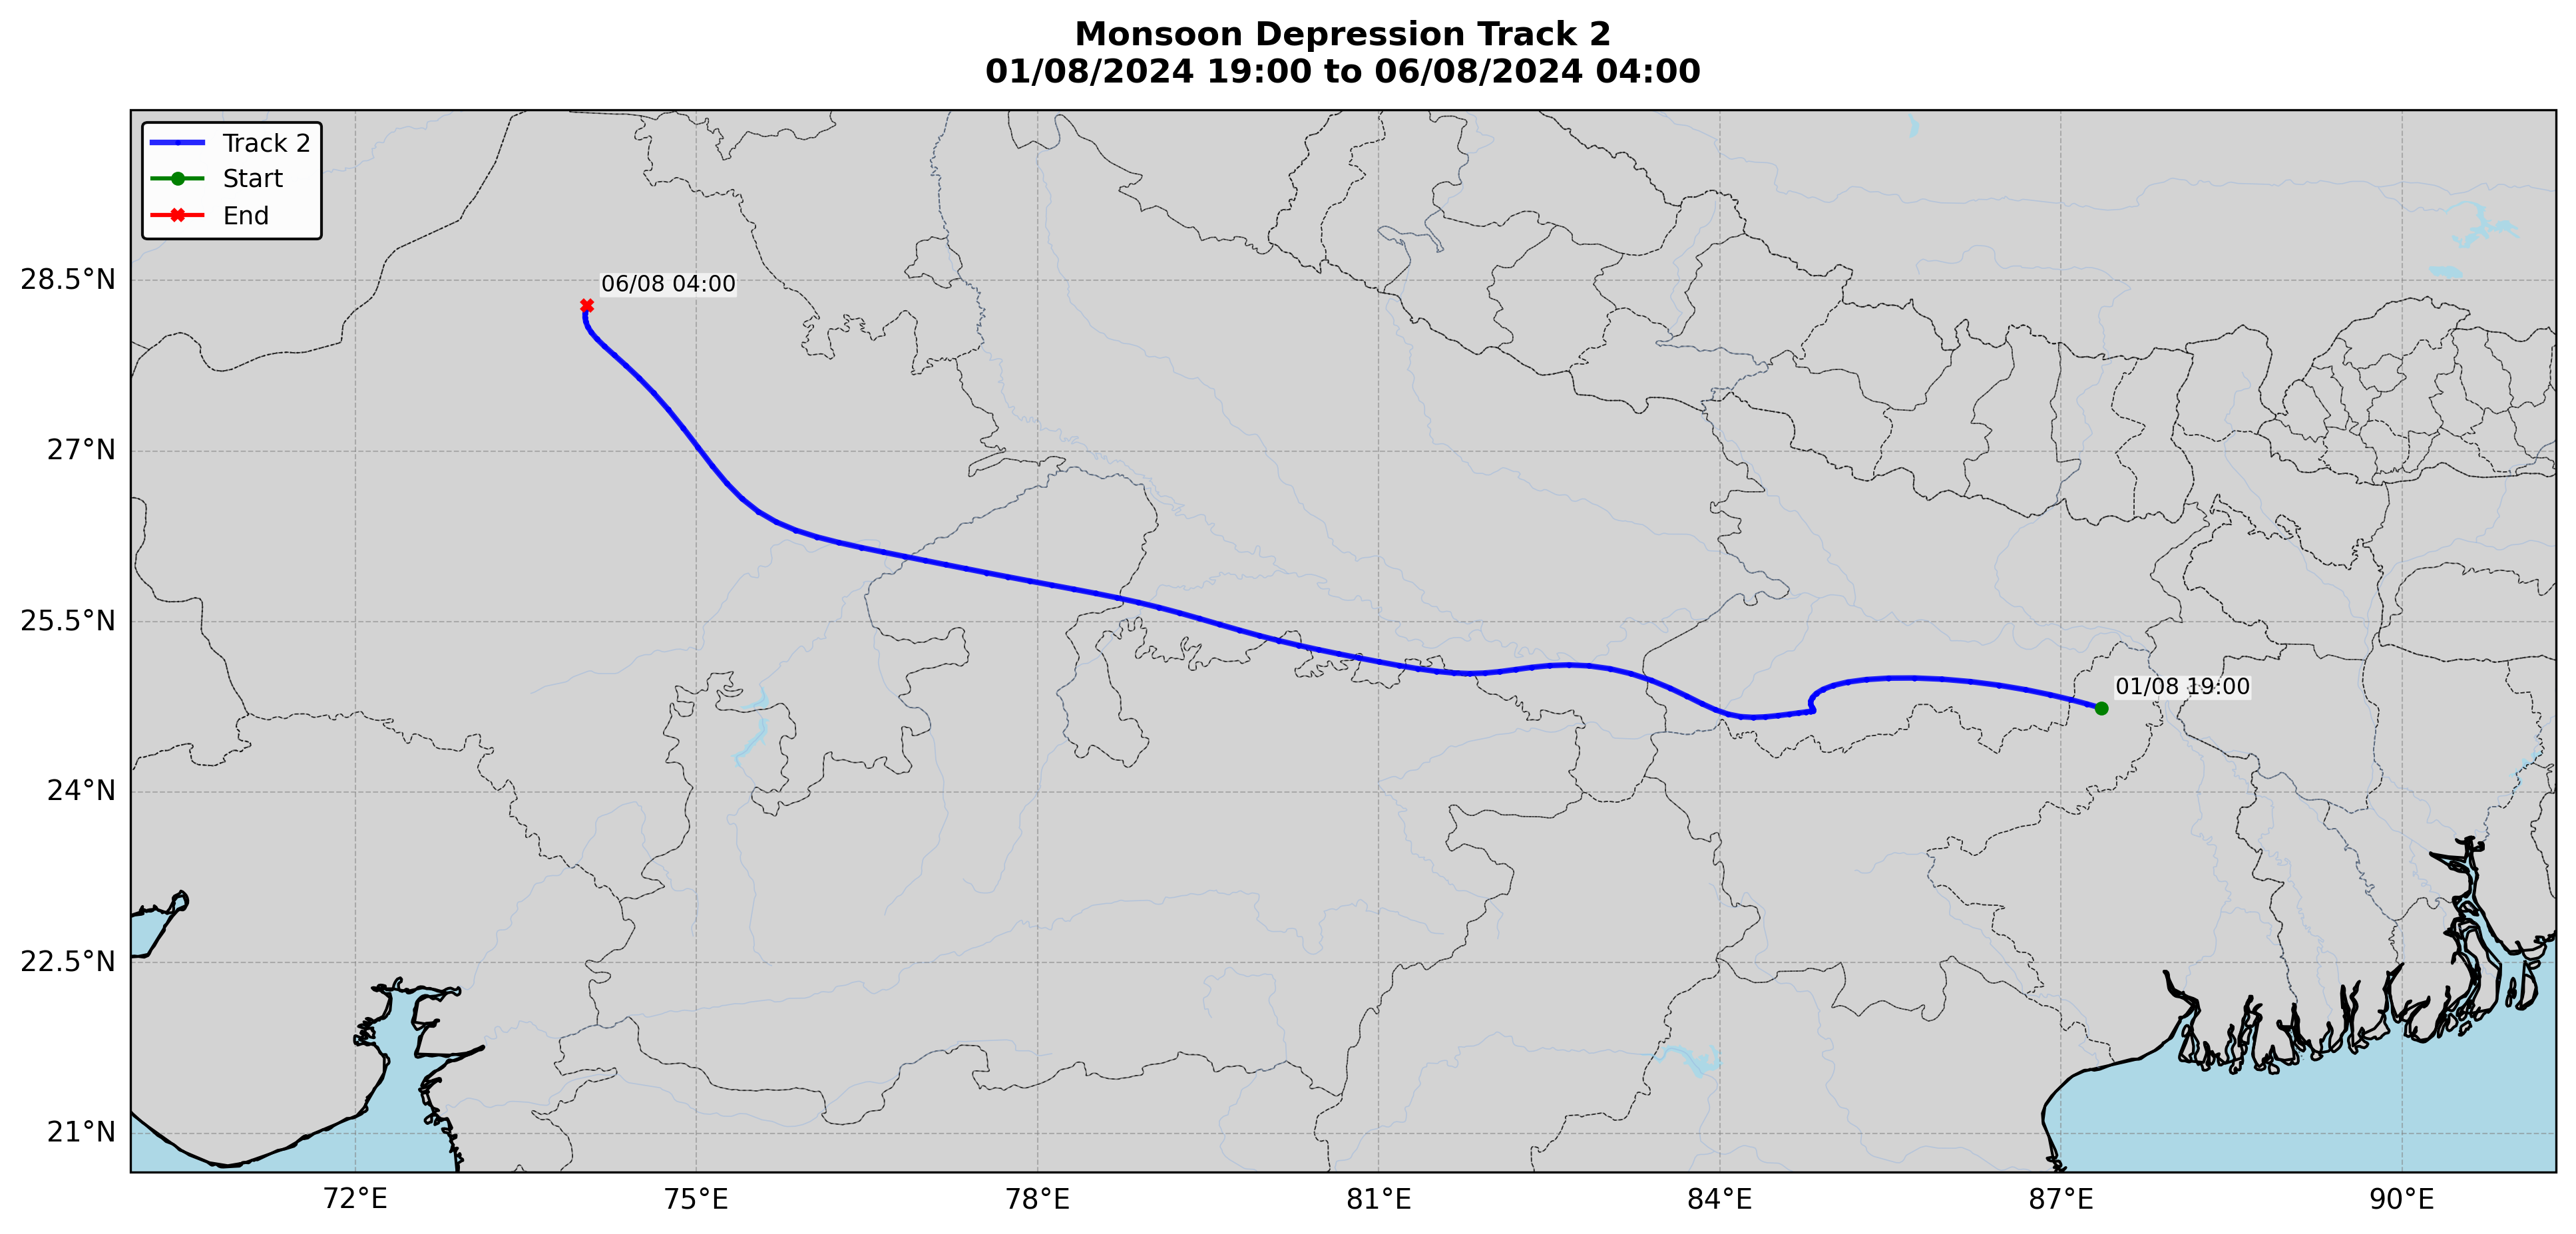
\includegraphics[width=0.95\textwidth]{../version5-with-no-ocean-masking/output/track_2/MD-track-2-detailed.png}

			\column{0.4\textwidth}
			\begin{block}{Statistics}
				\begin{itemize}
					\item Duration: 106 hours ($\sim$ 4.5 days)
					\item Category: long-lived MD
					\item Originated: over land
				\end{itemize}
			\end{block}
		\end{columns}
	\end{center}
\end{frame}

% 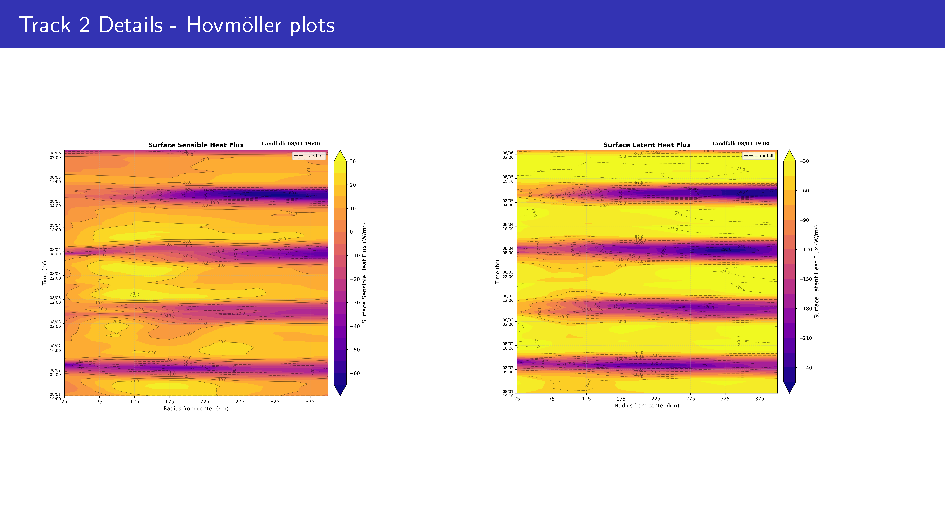
\includepdf[
% 	pages=-,
% 	scale=1,
% 	frame=true,
% 	pagecommand={\thispagestyle{empty}},  % Remove page numbers
% 	offset=0mm 0mm,       % Adjust position
% 	% templatesize={\textwidth}{\textheight} % Match template size
% ]{hovmoller-slides/hov-2.pdf}

% \begin{frame}{Track 2 Details - Precipitation and soil moisture over time along track}
% 	\begin{center}
% 		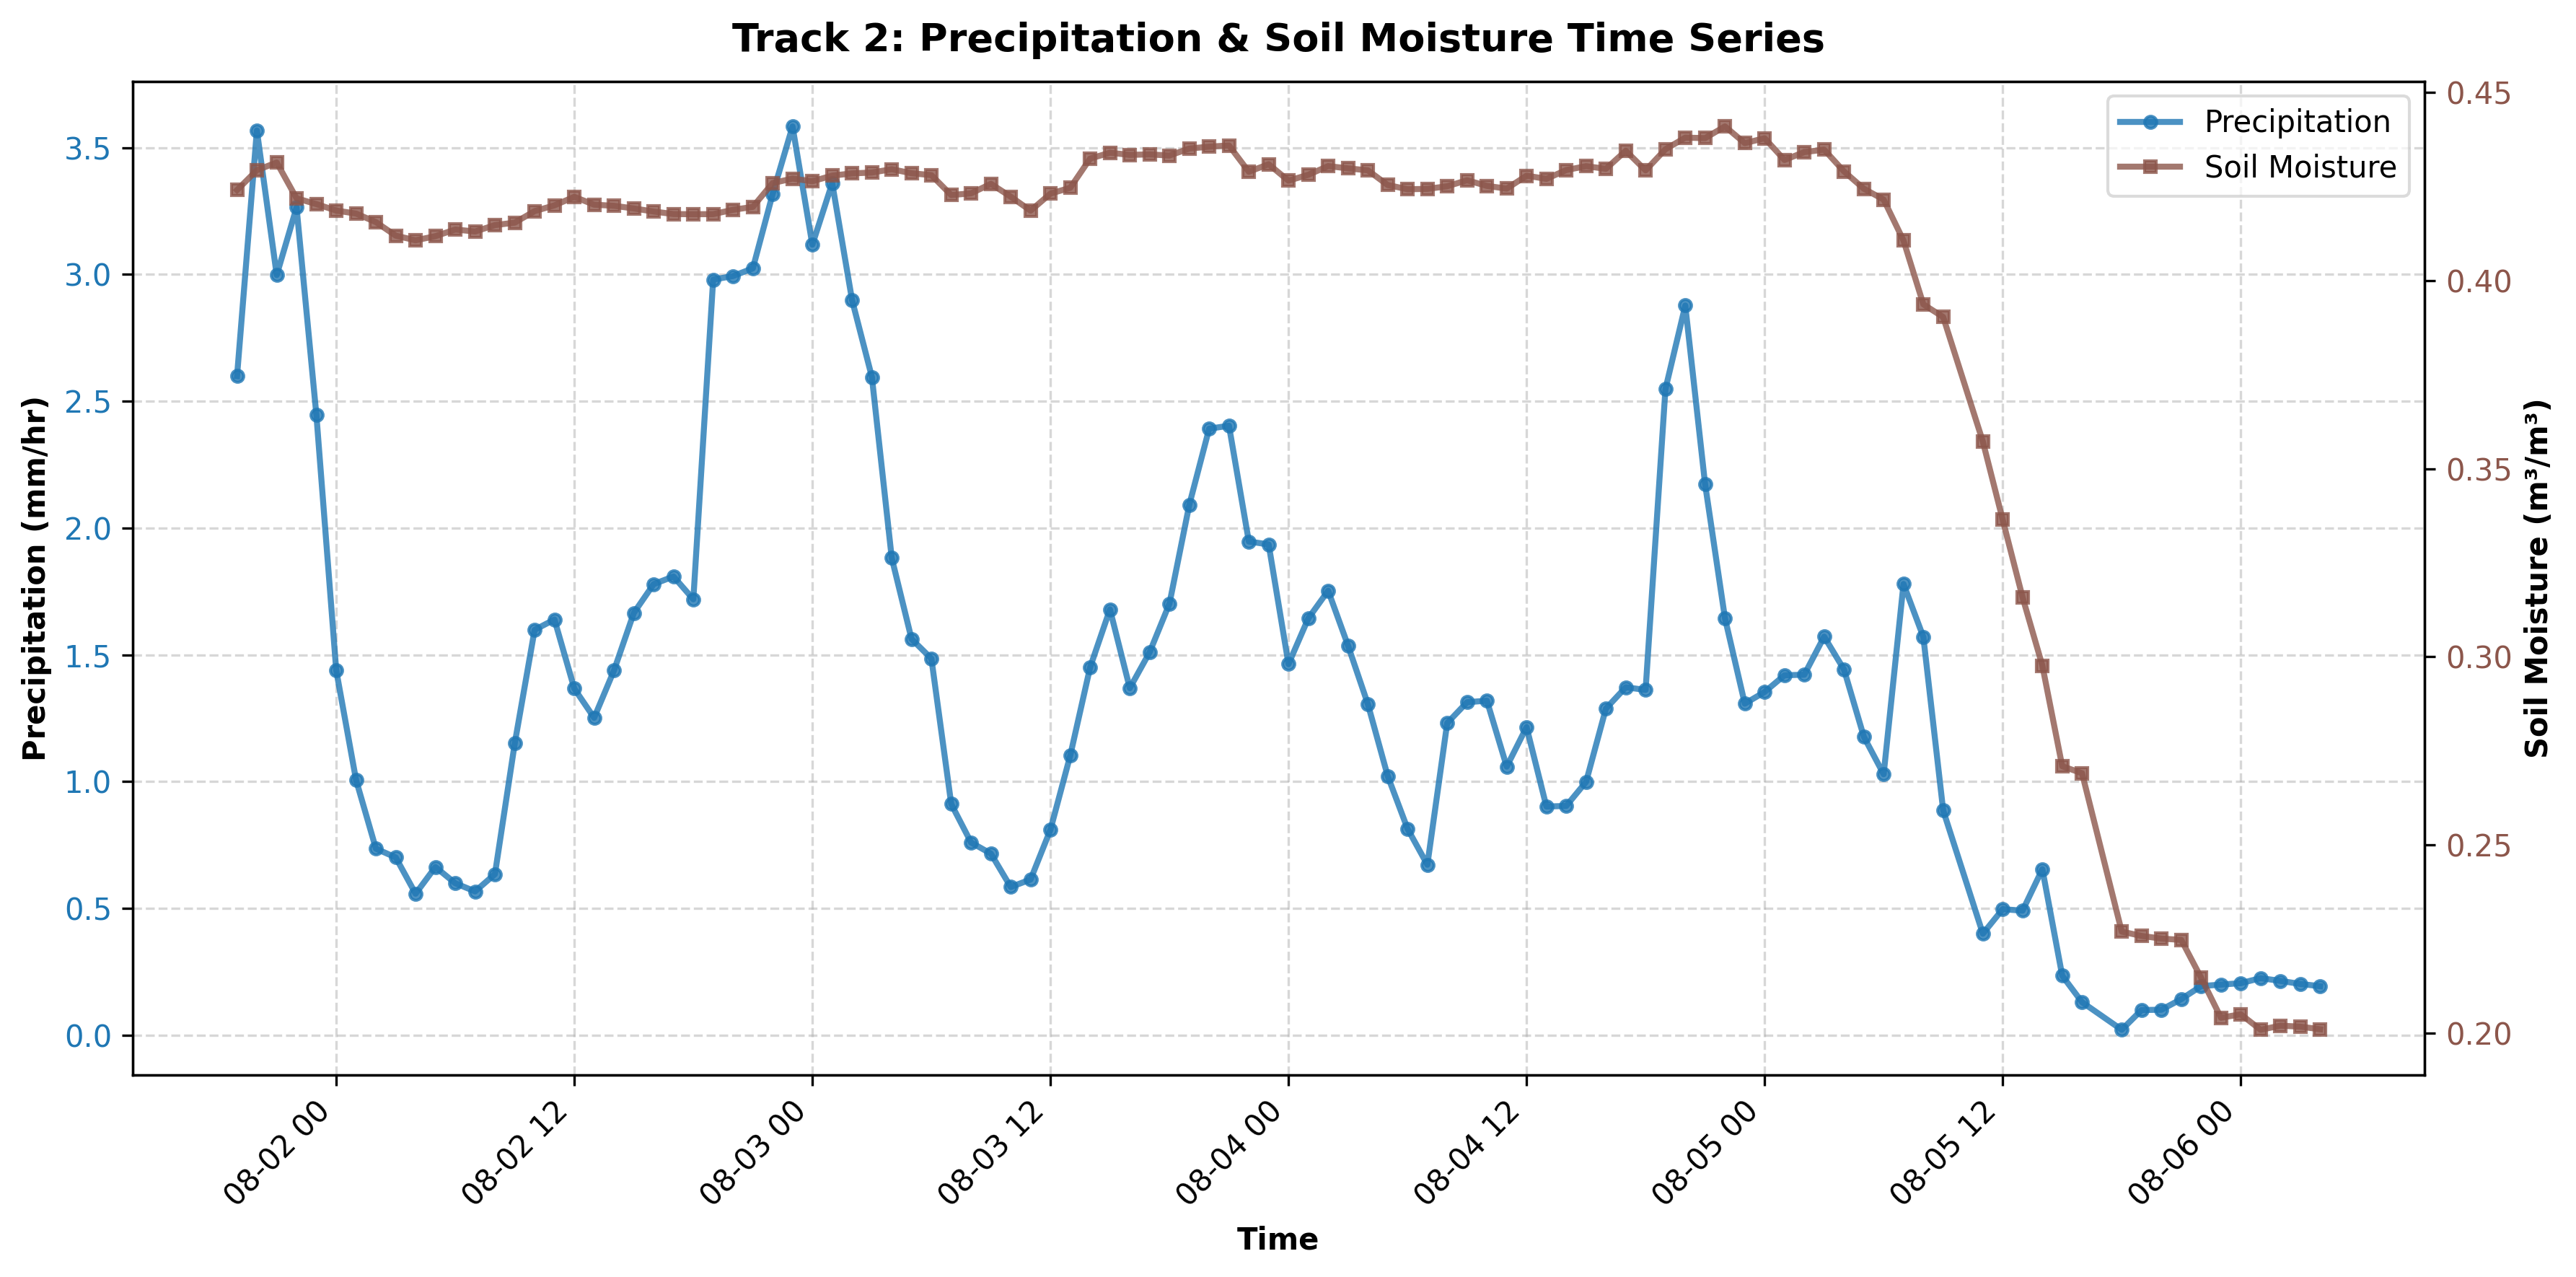
\includegraphics[width=0.8\textwidth]{../version1-with-no-ocean-masking/output/track_2/correlation_analysis/time_series/track_2_time_series.png}
% 	\end{center}
% \end{frame}

\begin{frame}{Track 2 Details - Translation speed of MD}
	\begin{center}
		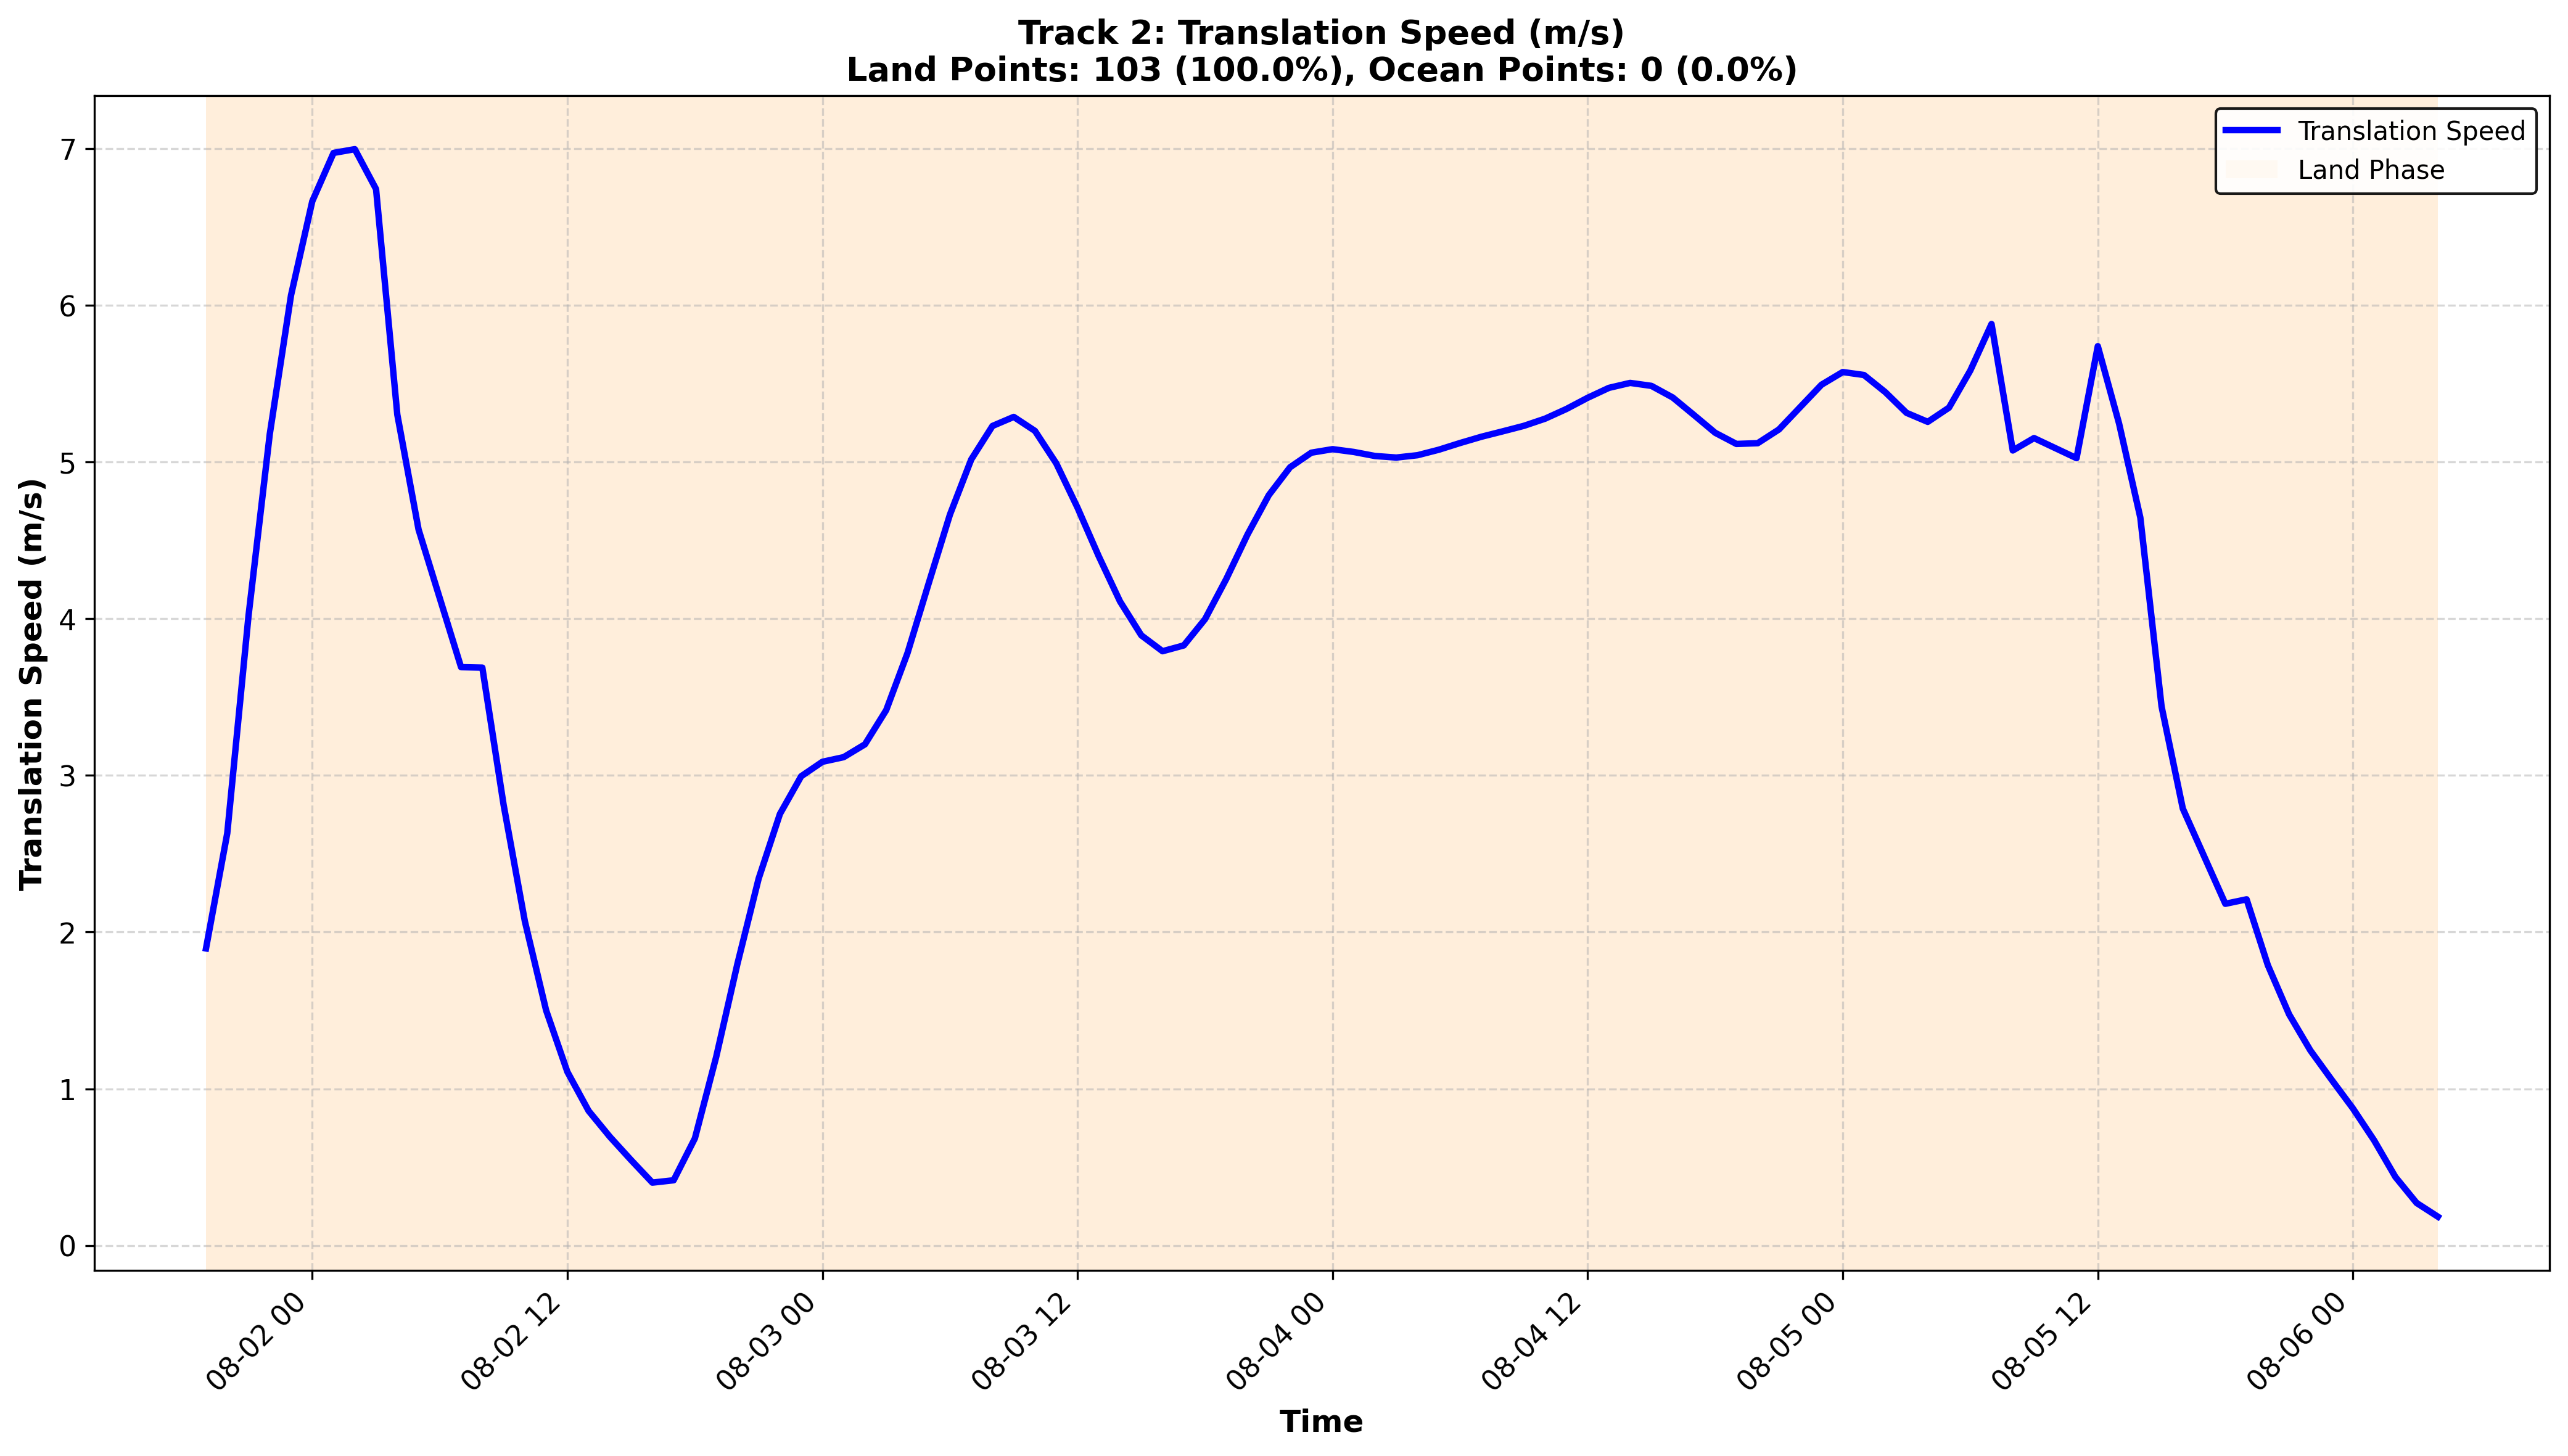
\includegraphics[width=0.8\textwidth]{../version5-with-no-ocean-masking/output/track_2/translational-speed/track_2_speed_ms.png}
	\end{center}
\end{frame}

\begin{frame}{Track 2 Details - Lag Correlation}
	\begin{center}
		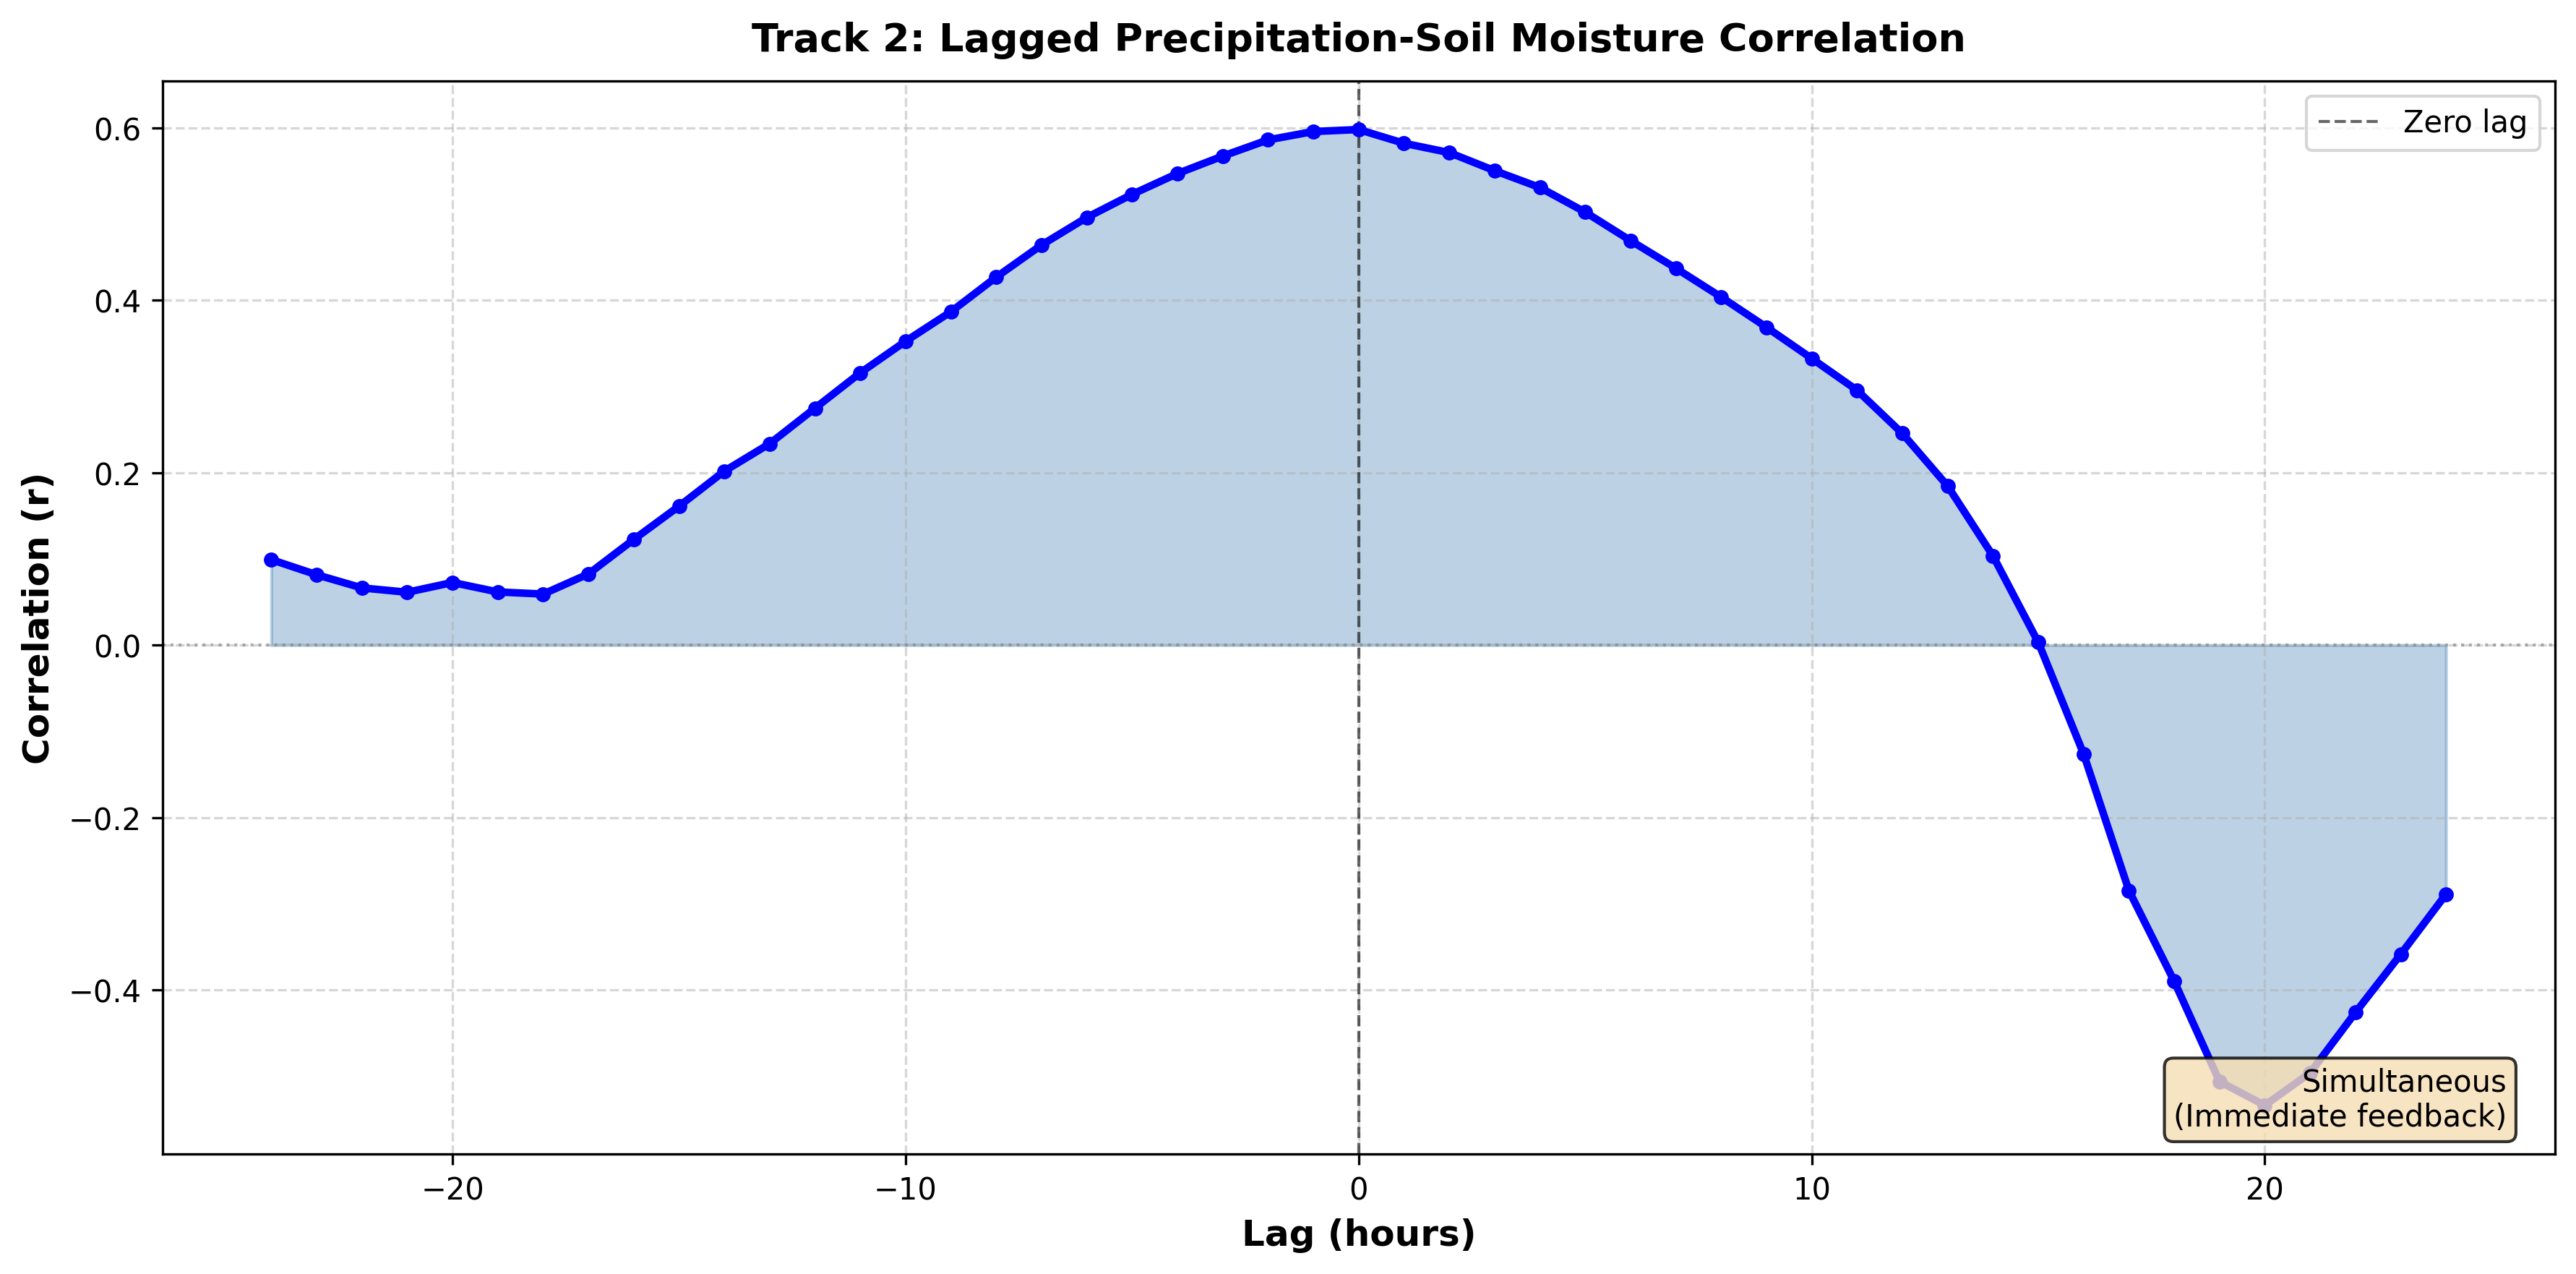
\includegraphics[width=0.8\textwidth]{../version5-with-no-ocean-masking/output/track_2/correlation_analysis/lag_correlation/track_2_lag_corr.png}
	\end{center}
\end{frame}

\begin{frame}{Track 2 Details - TP - SWVL1 Correlation}
	\begin{center}
		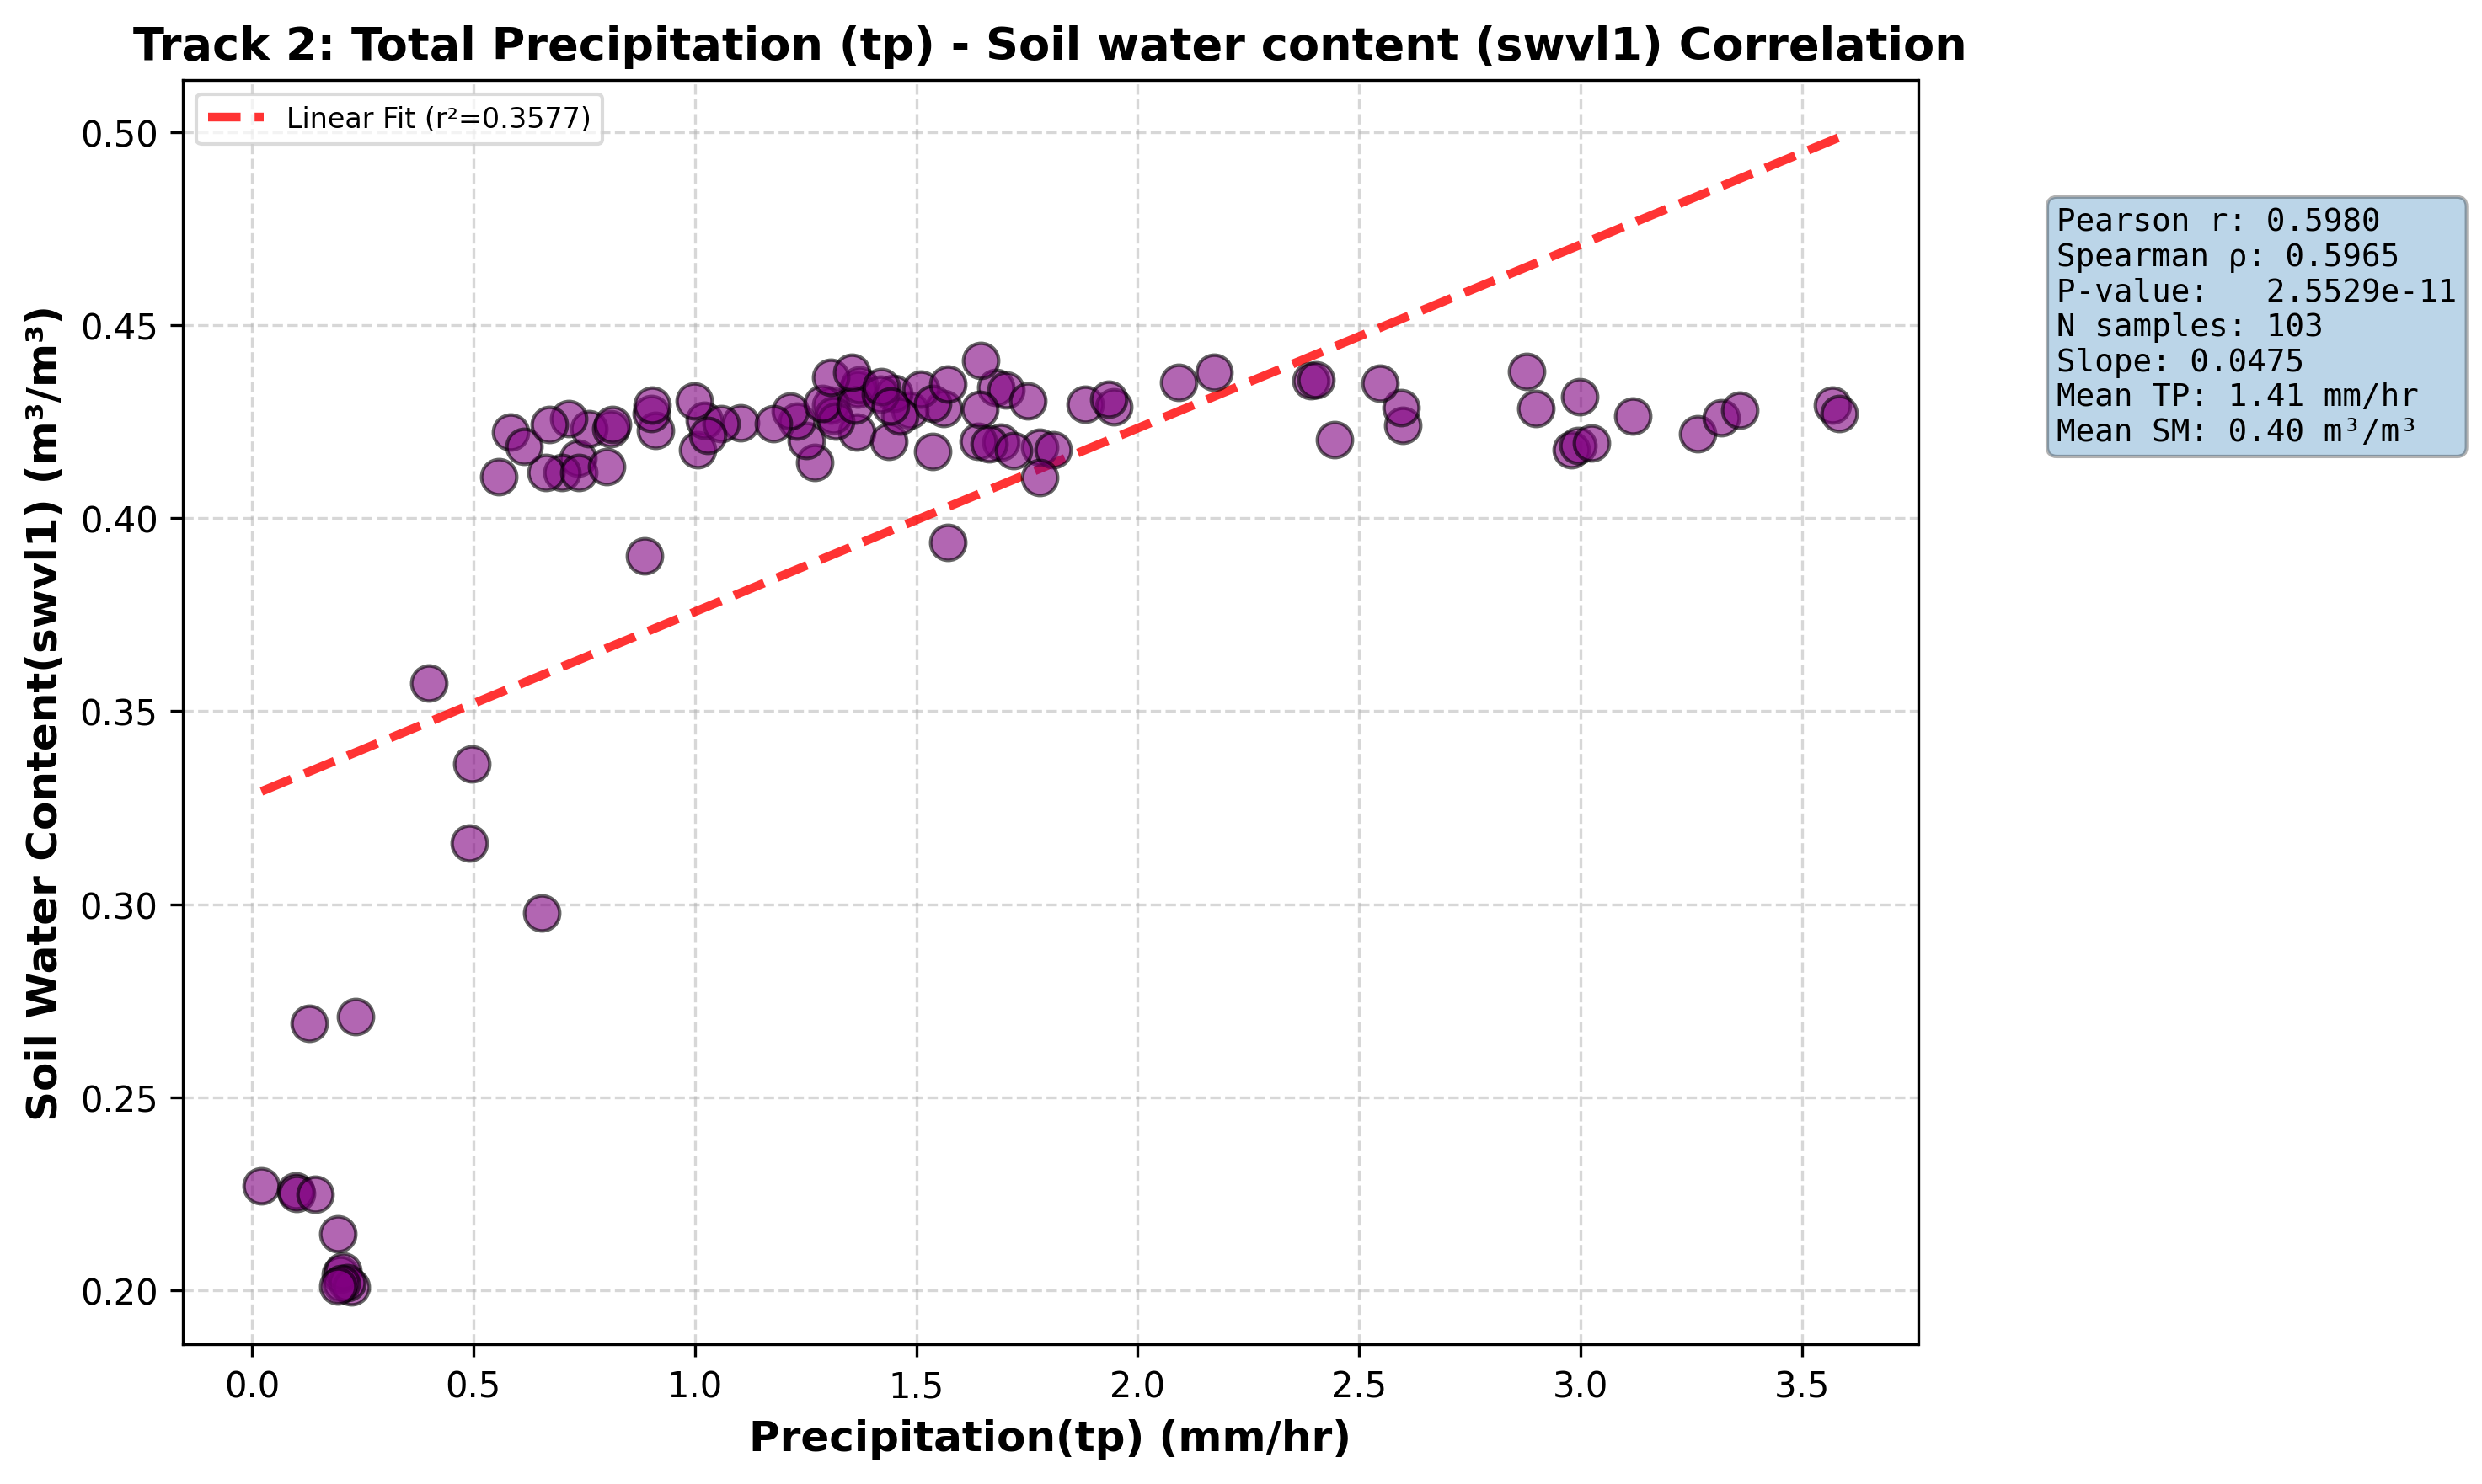
\includegraphics[width=0.7\textwidth]{../version5-with-no-ocean-masking/output/track_2/correlation_analysis/scatter_plots/track_2_scatter.png}
	\end{center}
\end{frame}

\begin{frame}{Track 2 Details - Spatial distribution of TP and SWVL1}
	\begin{center}
		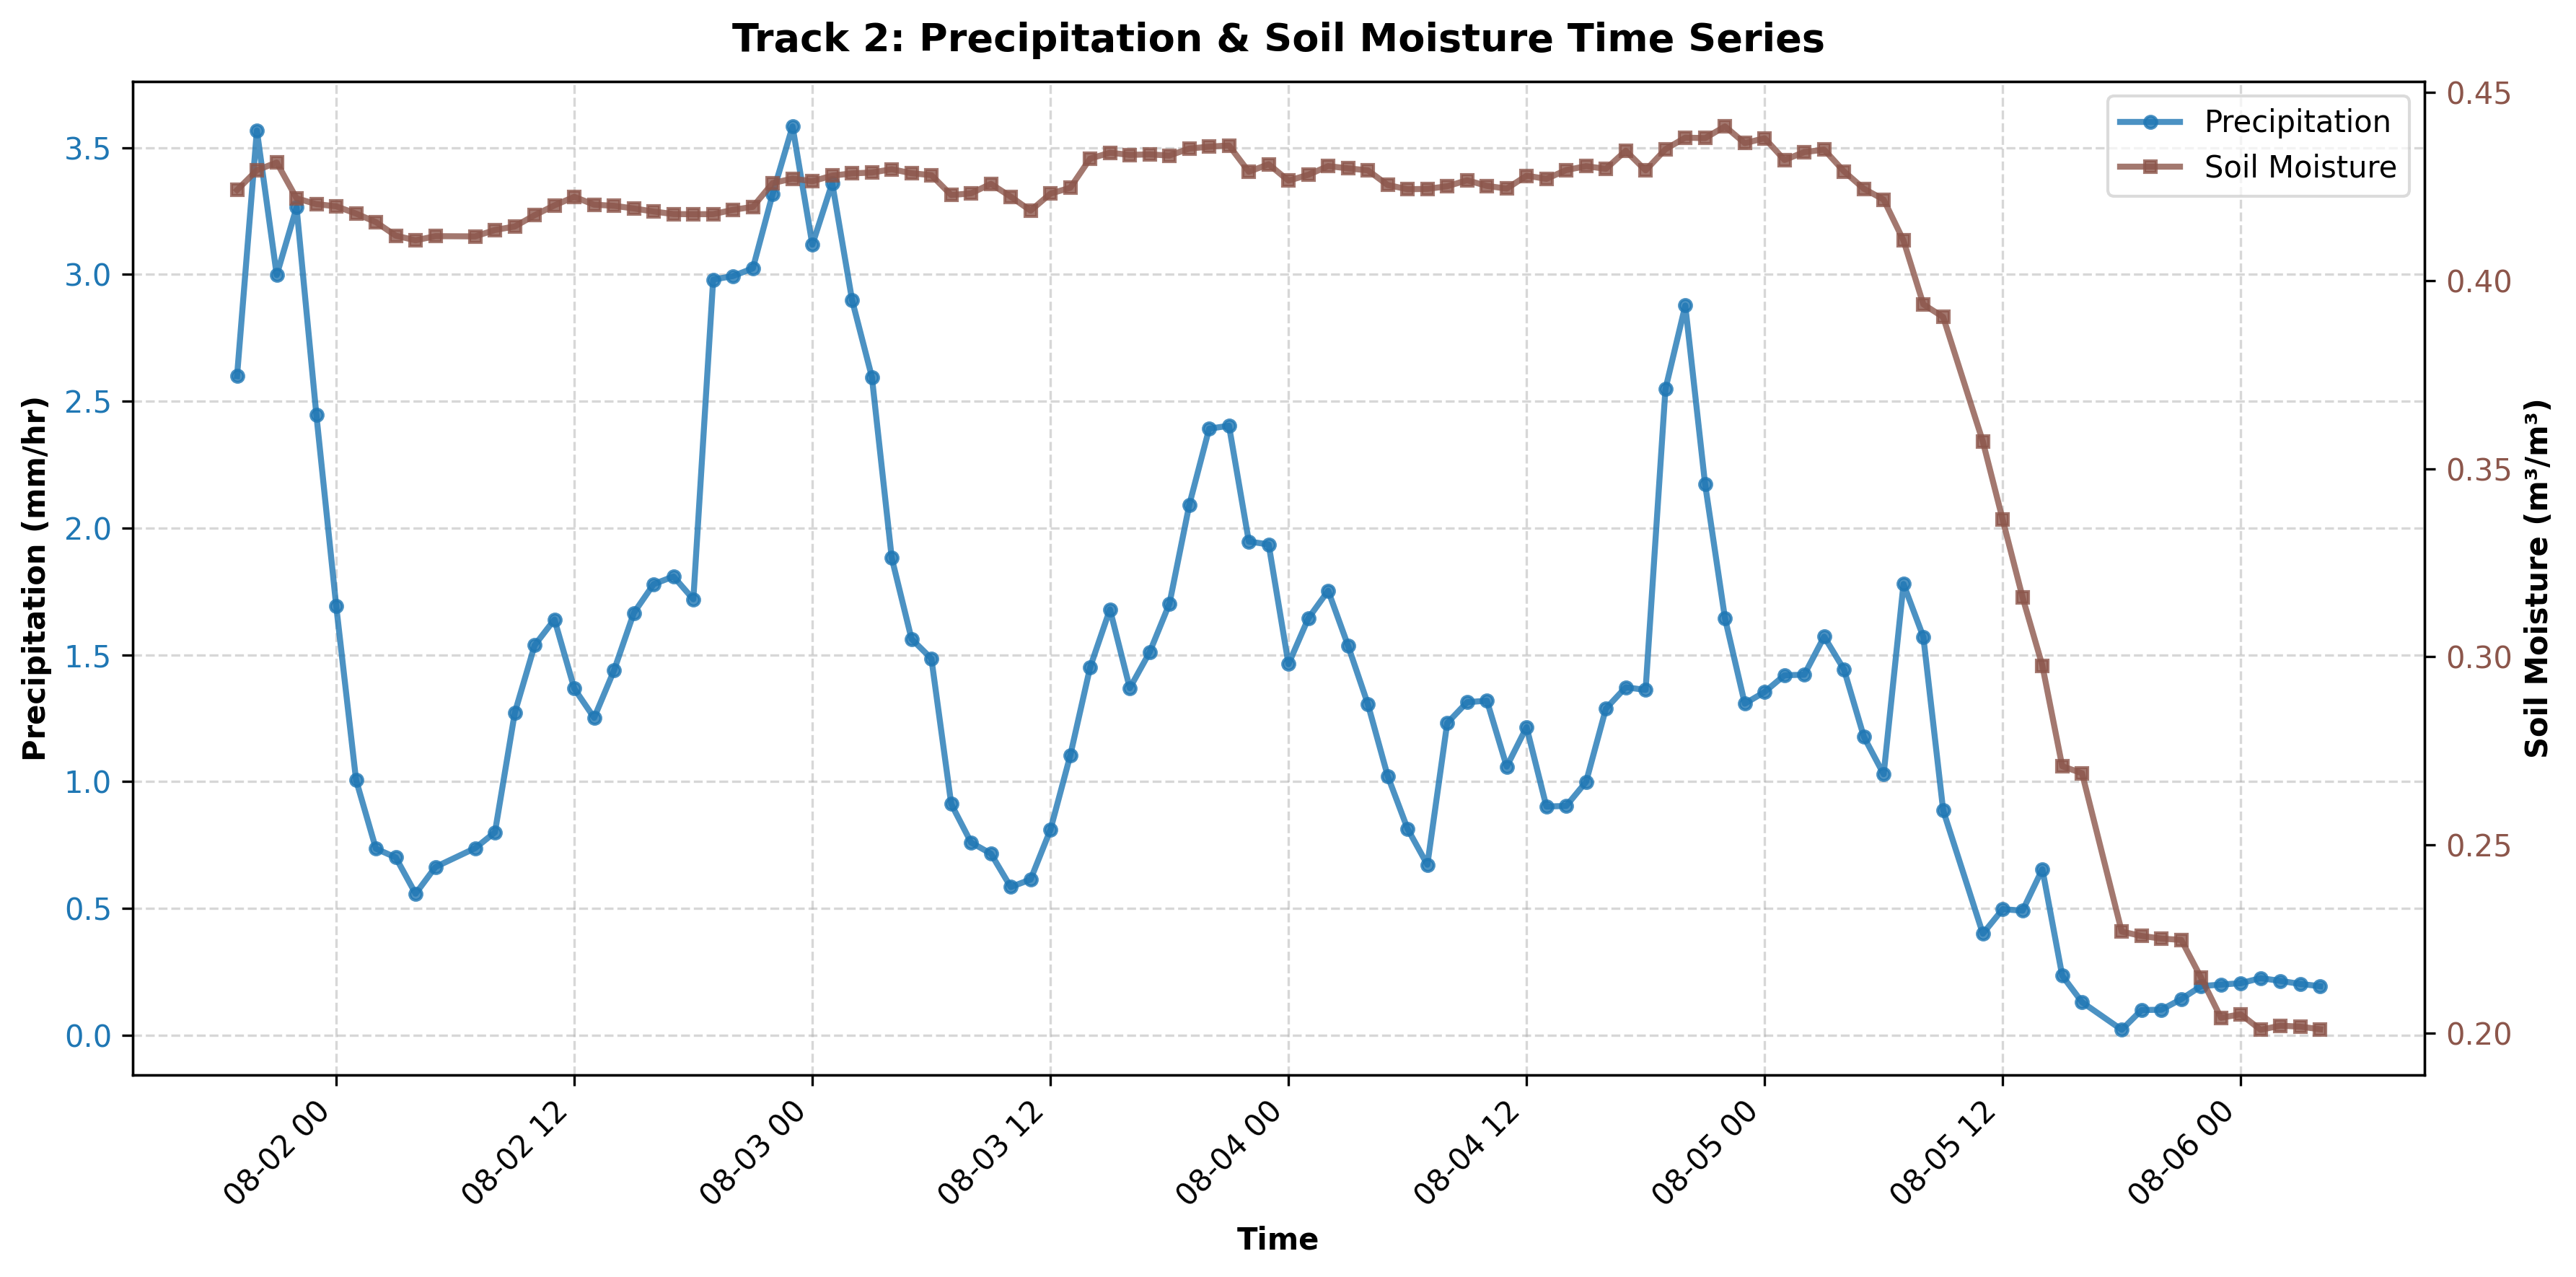
\includegraphics[width=0.7\textwidth]{../version5-with-no-ocean-masking/output/track_2/correlation_analysis/time_series/track_2_tp_sm_time_series.png}
	\end{center}
\end{frame}

% \begin{frame}{Track 2 Details - Heat fluxes transition}
% 	\begin{center}
% 		\includegraphics[width=0.8\textwidth]{../version5-with-no-ocean-masking/output/track_2/flux_analysis/track_2_analysis/track_2_heat_fluxes_trasnsition.png}
% 	\end{center}
% \end{frame}

\begin{frame}{Track 2 Details - Heat flux analysis}
	\begin{center}
		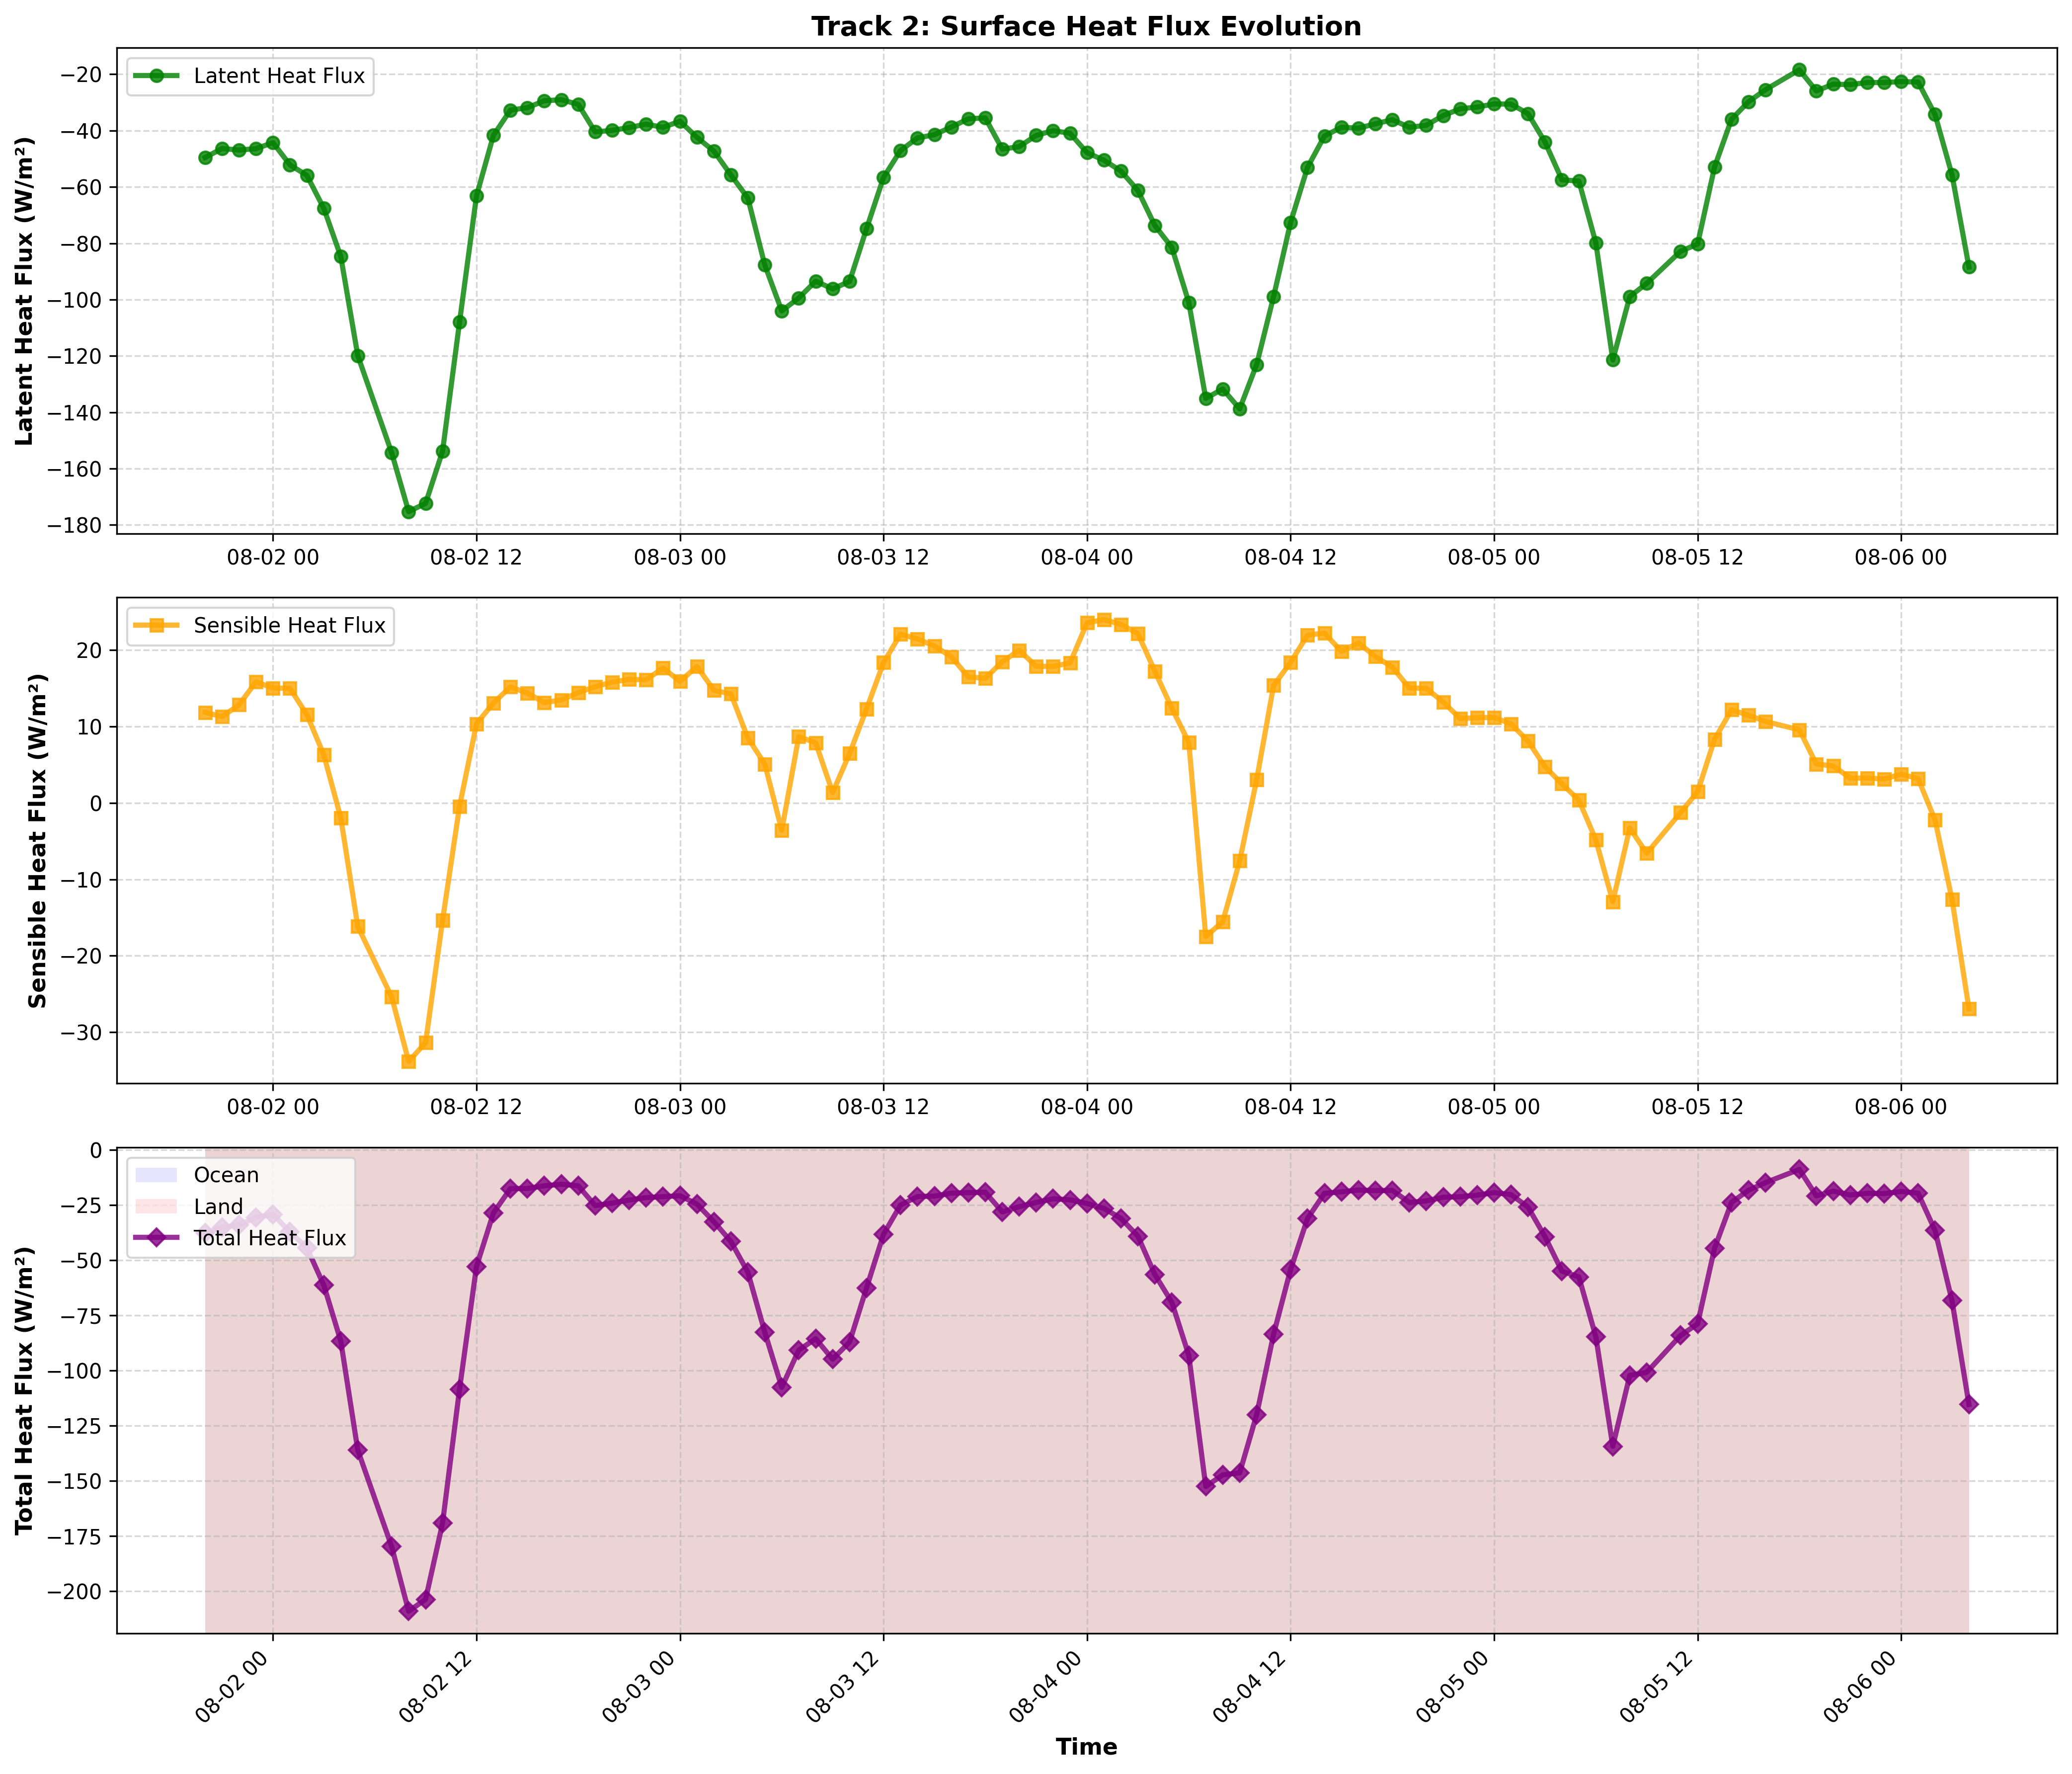
\includegraphics[width=0.6\textwidth]{../version5-with-no-ocean-masking/output/track_2/heat_flux_analysis/track_2_heat_flux_timeseries.png}
	\end{center}
\end{frame}

% %%%%%%%%%%%%%%%% Track 3 %%%%%%%%%%%%%%
\begin{frame}{Track 3 Details}
	\begin{center}
		\begin{columns}[T]
			\column{0.6\textwidth}
			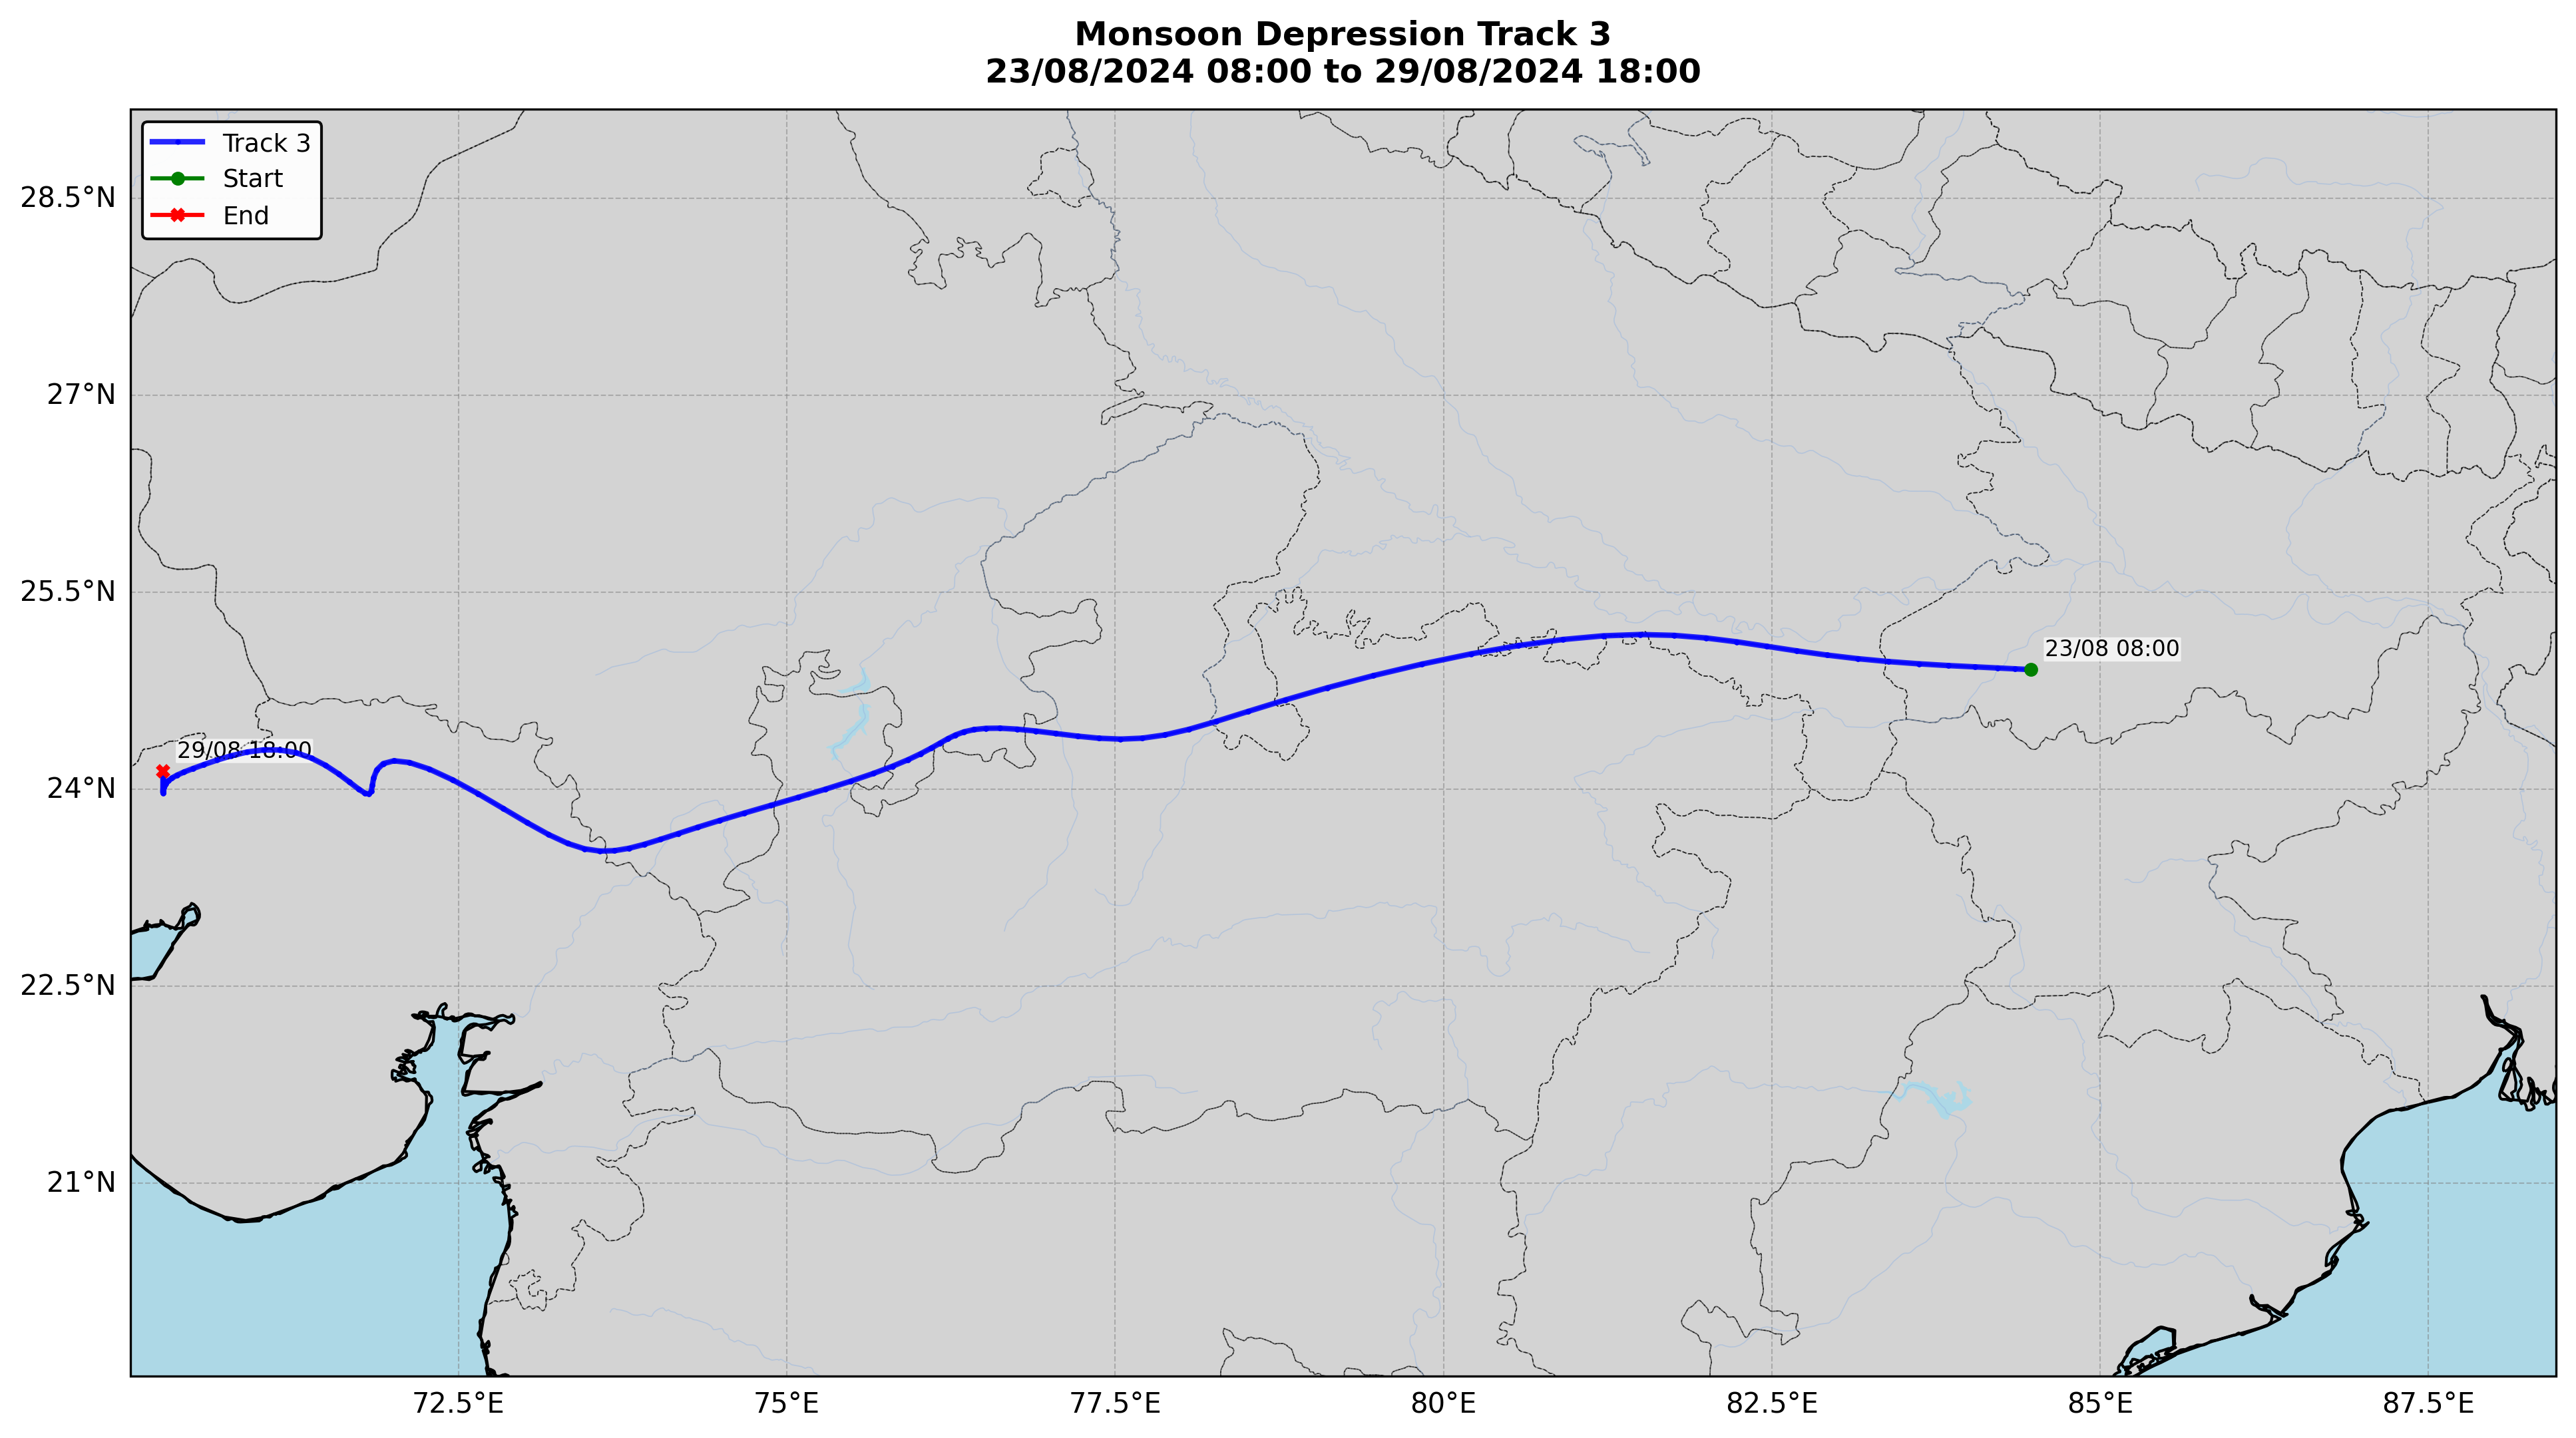
\includegraphics[width=0.95\textwidth]{../version5-with-no-ocean-masking/output/track_3/MD-track-3-detailed.png}

			\column{0.4\textwidth}
			\begin{block}{Statistics}
				\begin{itemize}
					\item Duration: 146 hours ($\sim$ 6 days)
					\item Category: long-lived MD
					\item Originated: over land
				\end{itemize}
			\end{block}
		\end{columns}
	\end{center}
\end{frame}

% 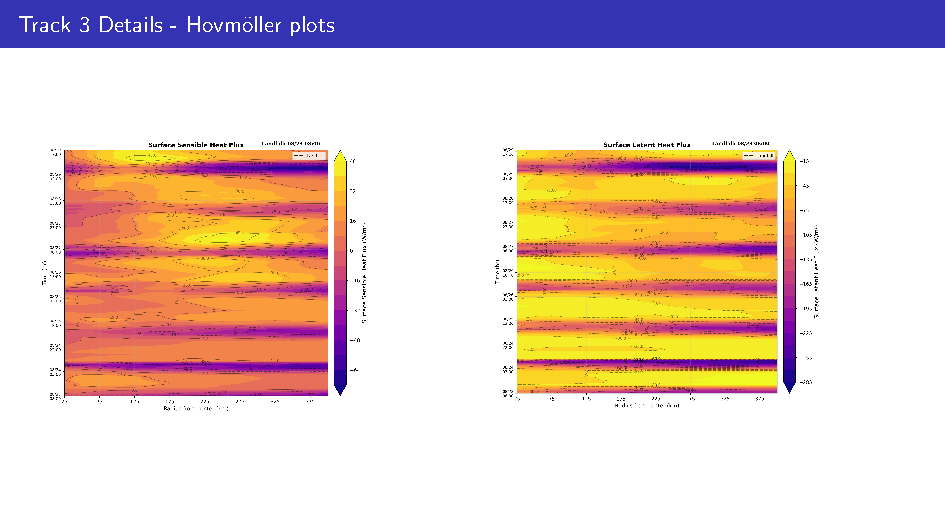
\includepdf[
% 	pages=-,
% 	scale=1,
% 	frame=true,
% 	pagecommand={\thispagestyle{empty}},  % Remove page numbers
% 	offset=0mm 0mm,       % Adjust position
% 	% templatesize={\textwidth}{\textheight} % Match template size
% ]{hovmoller-slides/hov-3.pdf}

% \begin{frame}{Track 3 Details - Precipitation and soil moisture over time along track}
% 	\begin{center}
% 		\includegraphics[width=0.8\textwidth]{../version5-with-no-ocean-masking/output/track_3/correlation_analysis/time_series/track_3_time_series.png}
% 	\end{center}
% \end{frame}

\begin{frame}{Track 3 Details - Translation speed of MD}
	\begin{center}
		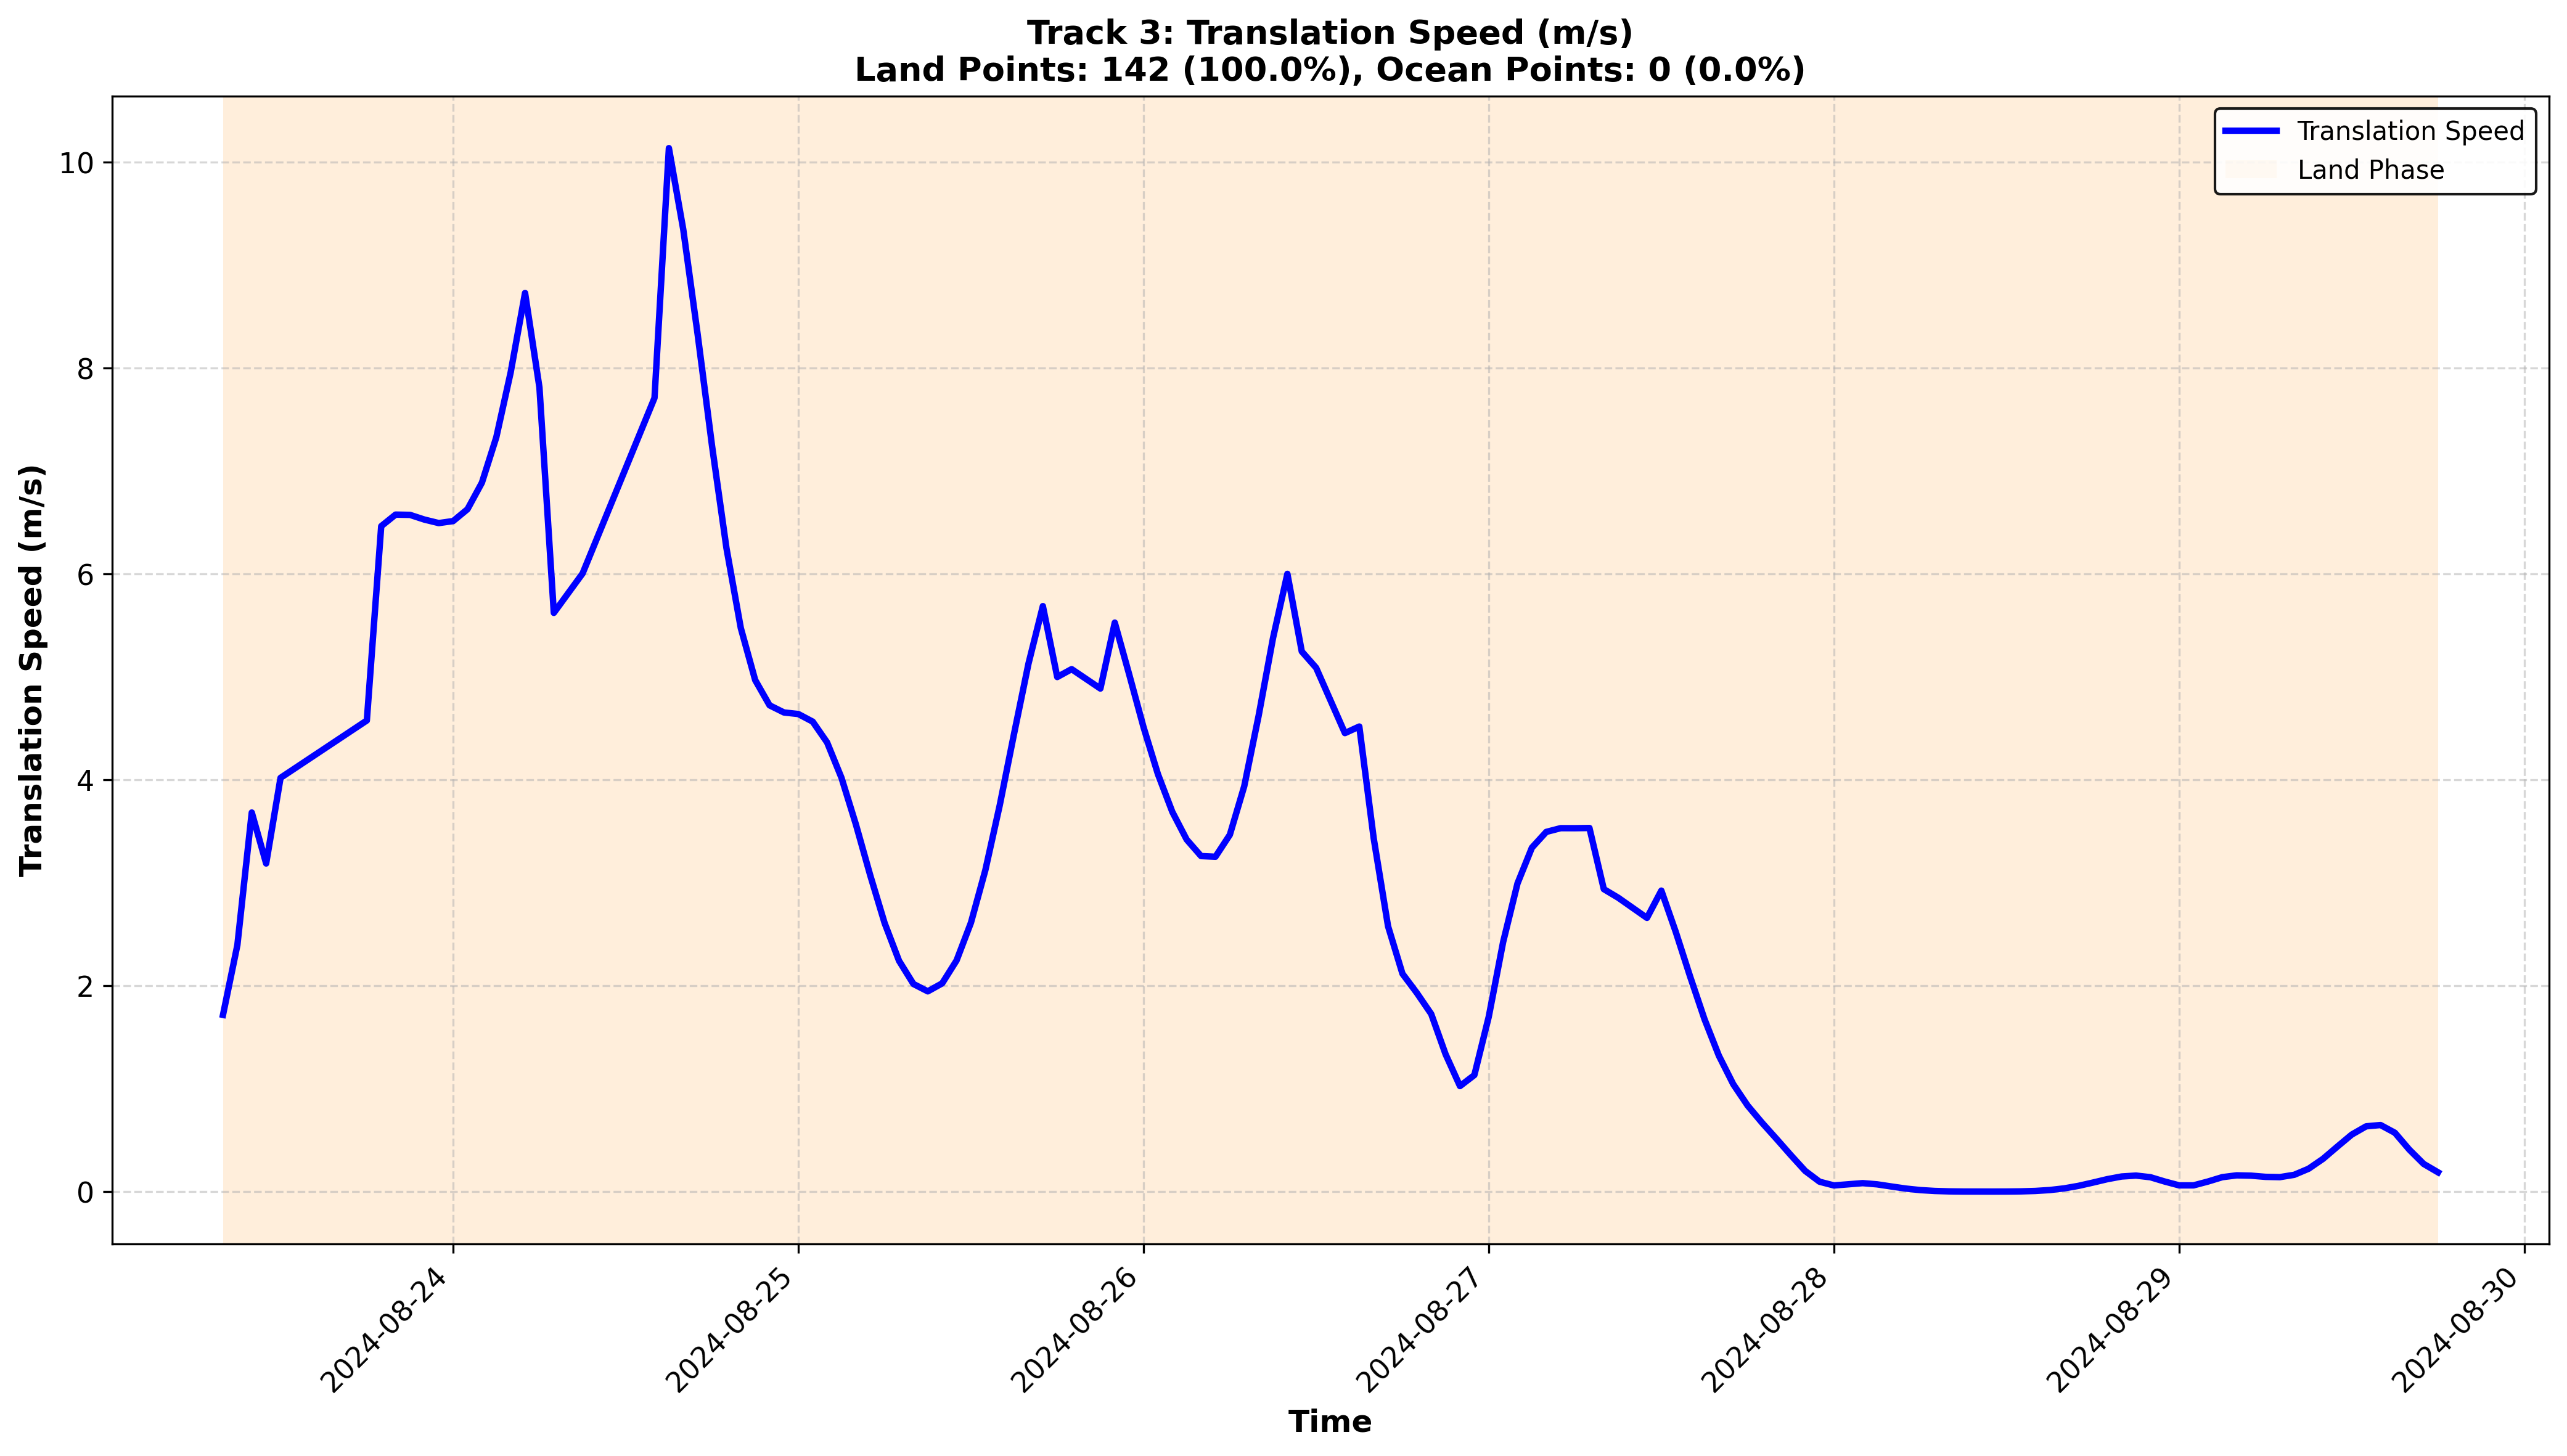
\includegraphics[width=0.8\textwidth]{../version5-with-no-ocean-masking/output/track_3/translational-speed/track_3_speed_ms.png}
	\end{center}
\end{frame}

\begin{frame}{Track 3 Details - Lag Correlation}
	\begin{center}
		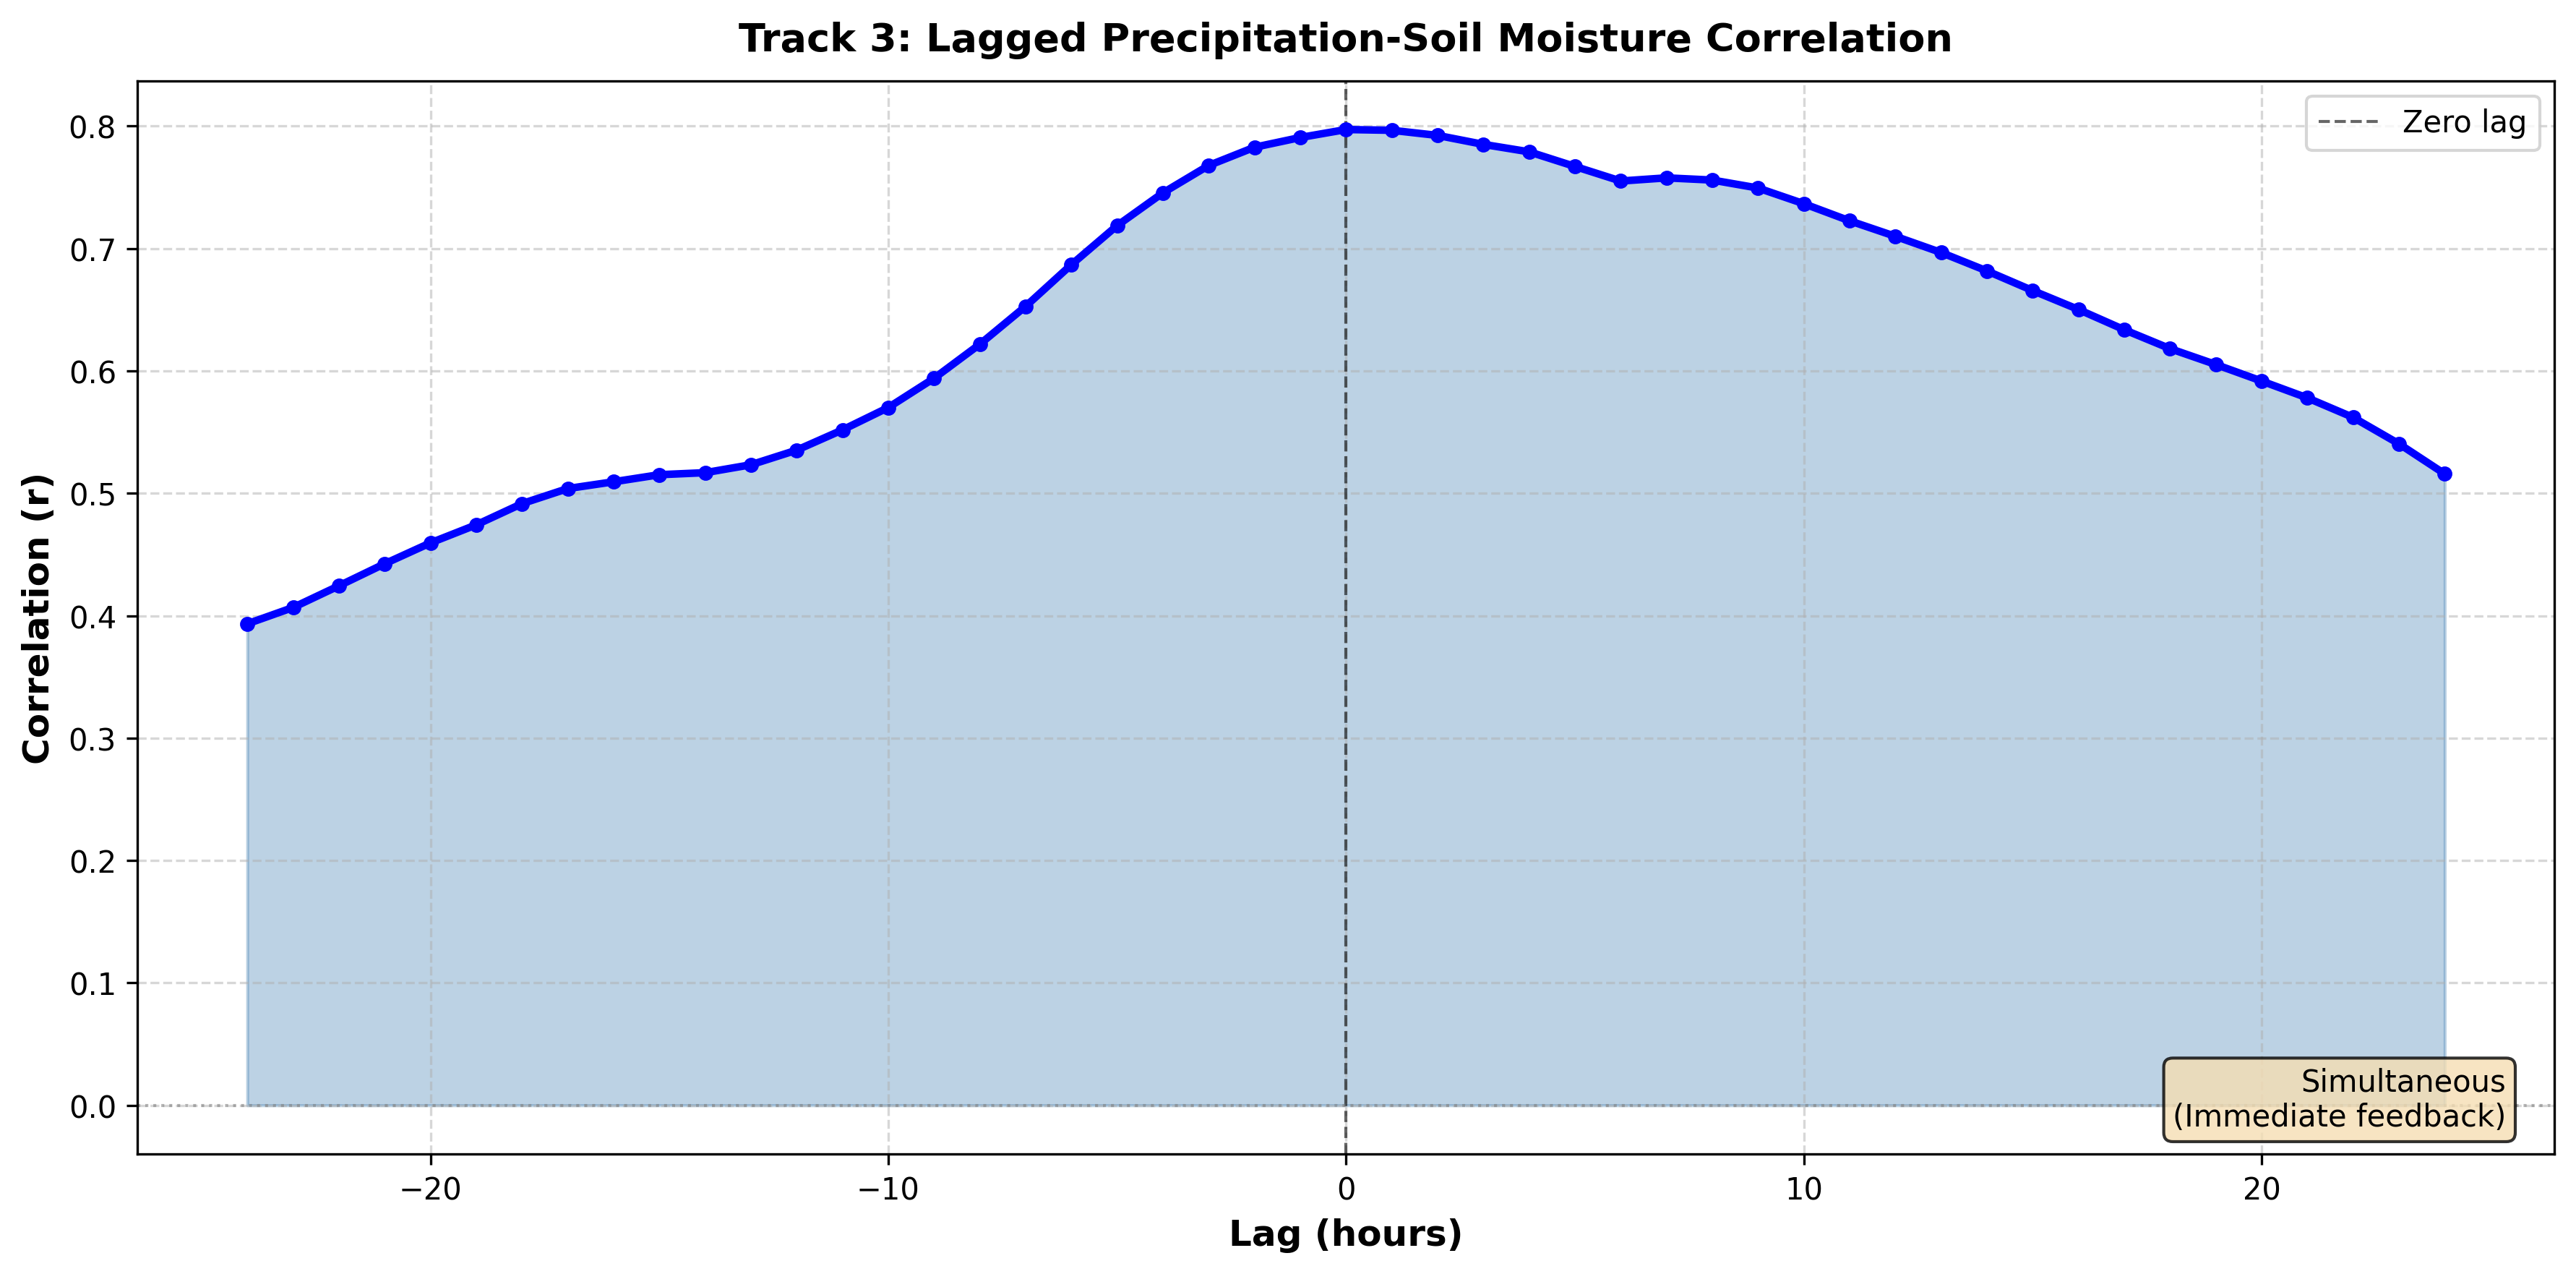
\includegraphics[width=0.8\textwidth]{../version5-with-no-ocean-masking/output/track_3/correlation_analysis/lag_correlation/track_3_lag_corr.png}
	\end{center}
\end{frame}

\begin{frame}{Track 3 Details - TP - SWVL1 Correlation}
	\begin{center}
		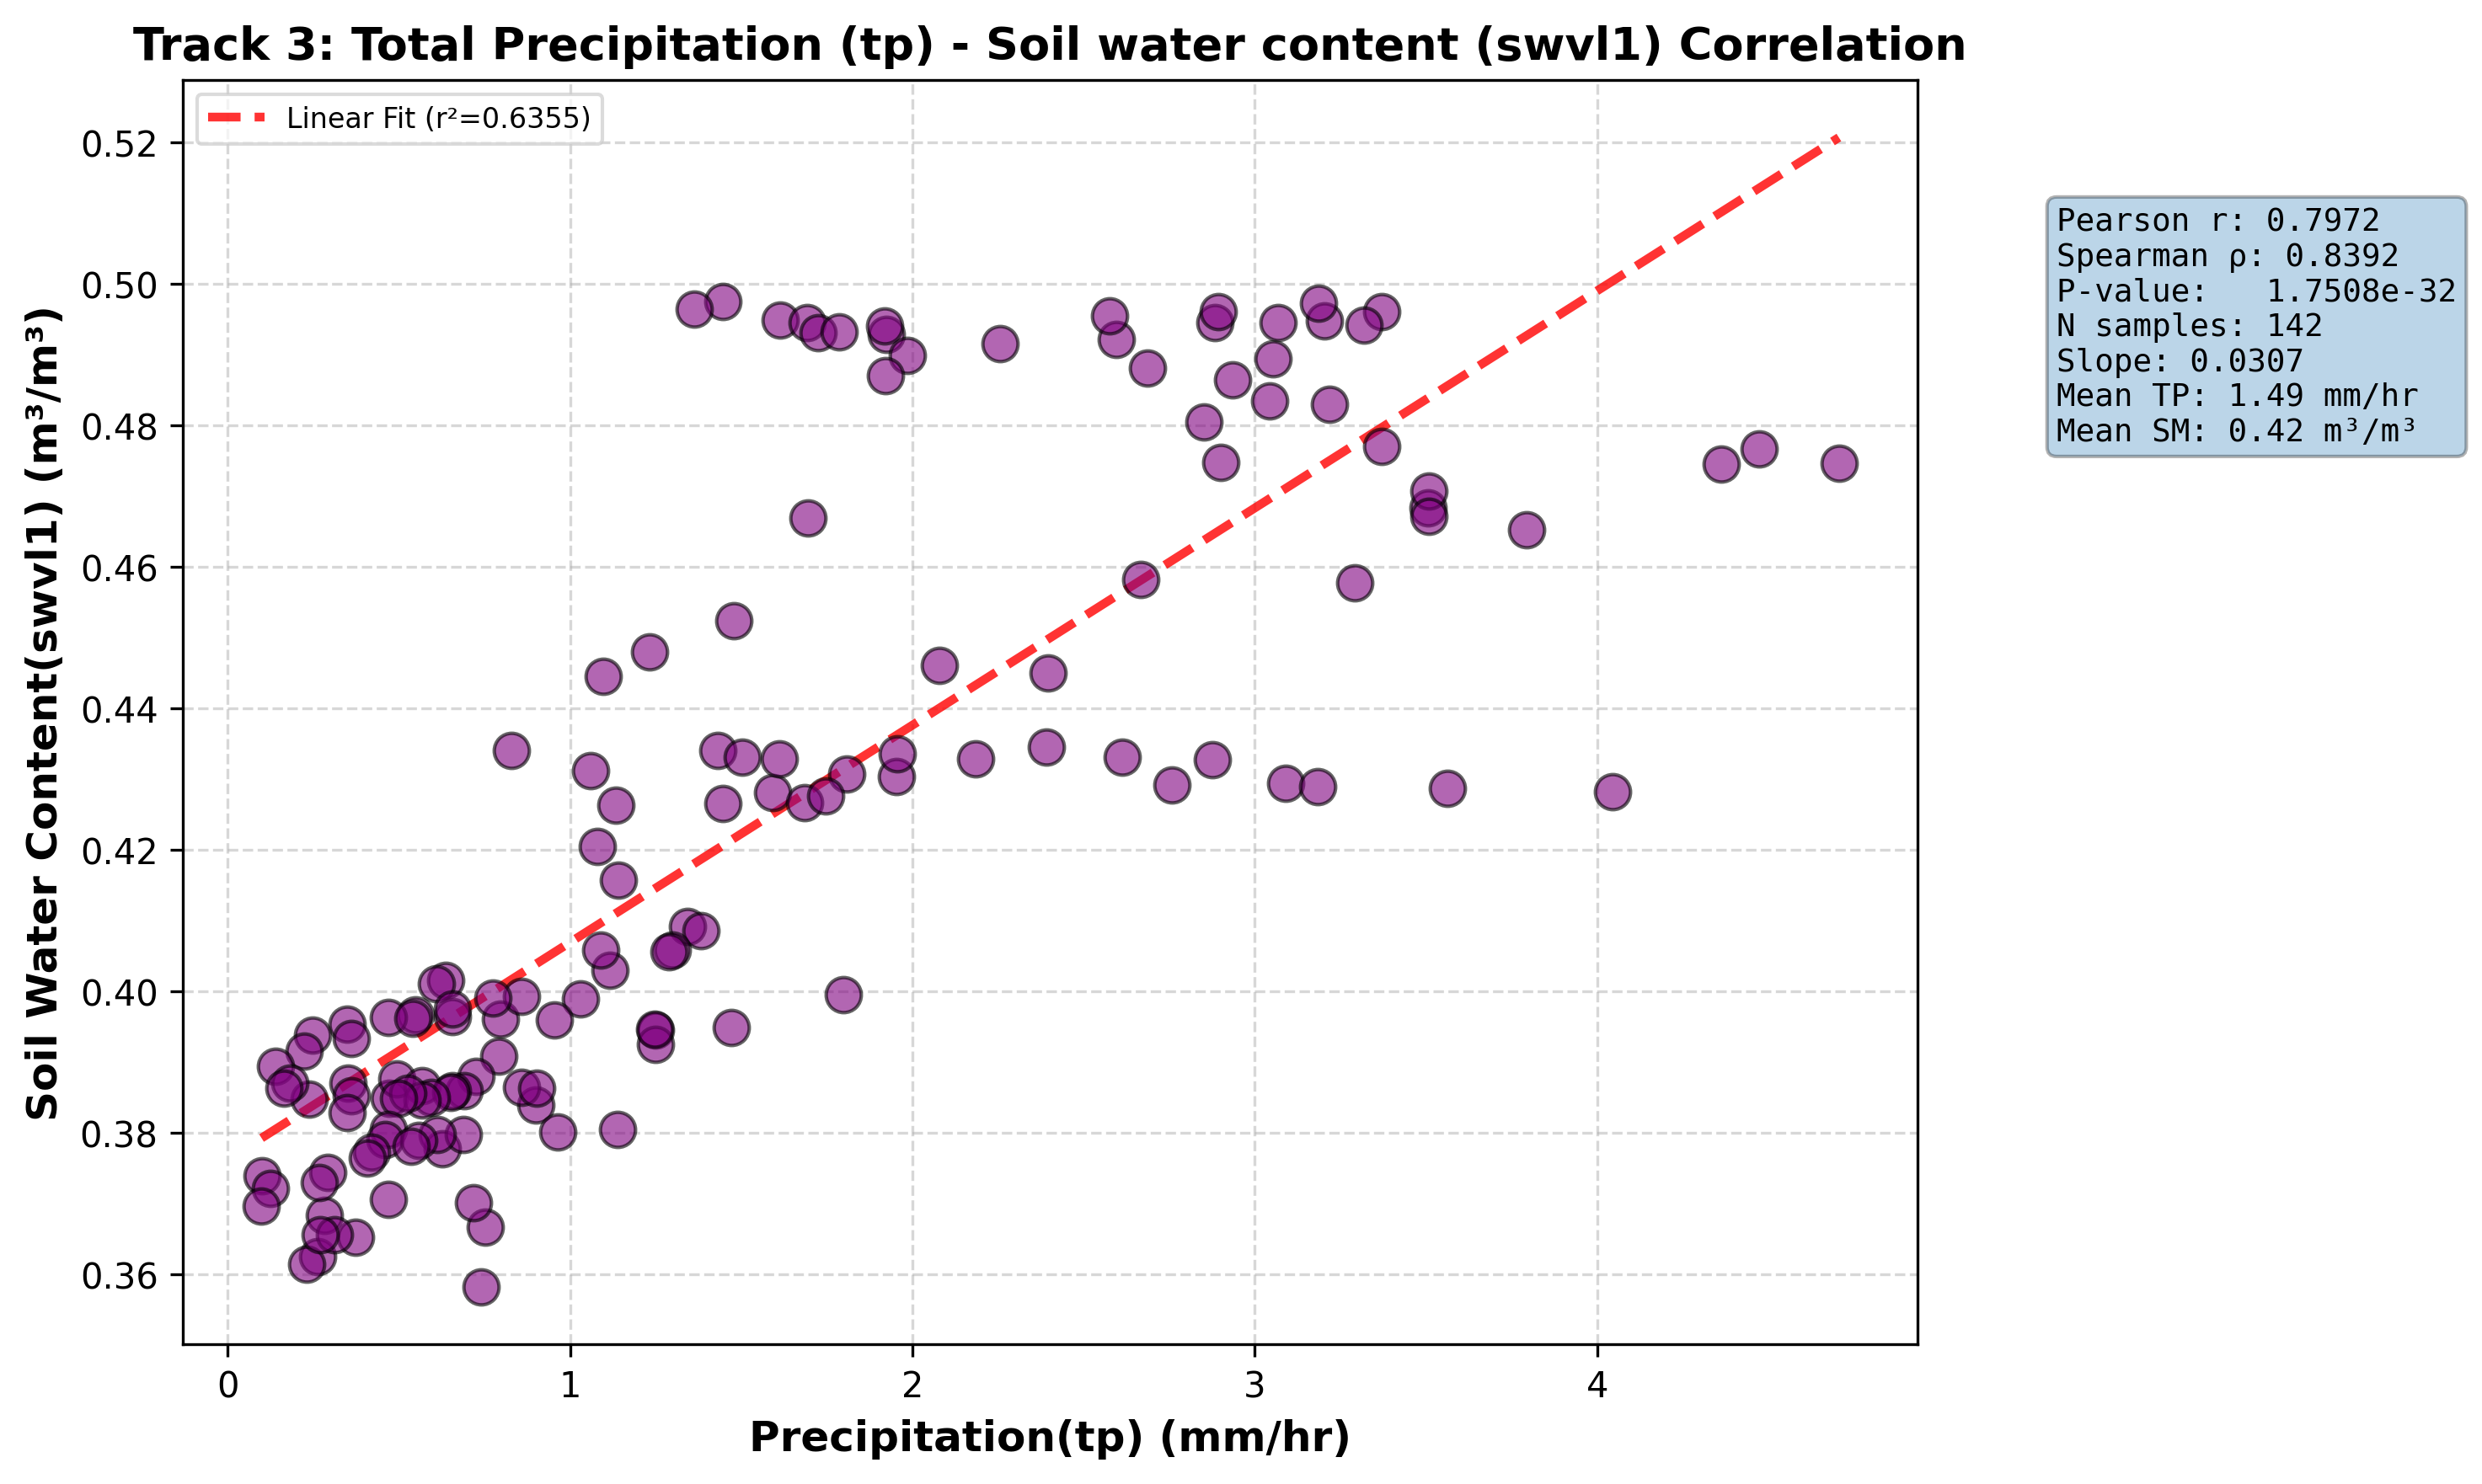
\includegraphics[width=0.7\textwidth]{../version5-with-no-ocean-masking/output/track_3/correlation_analysis/scatter_plots/track_3_scatter.png}
	\end{center}
\end{frame}

\begin{frame}{Track 3 Details - Spatial distribution of TP and SWVL1}
	\begin{center}
		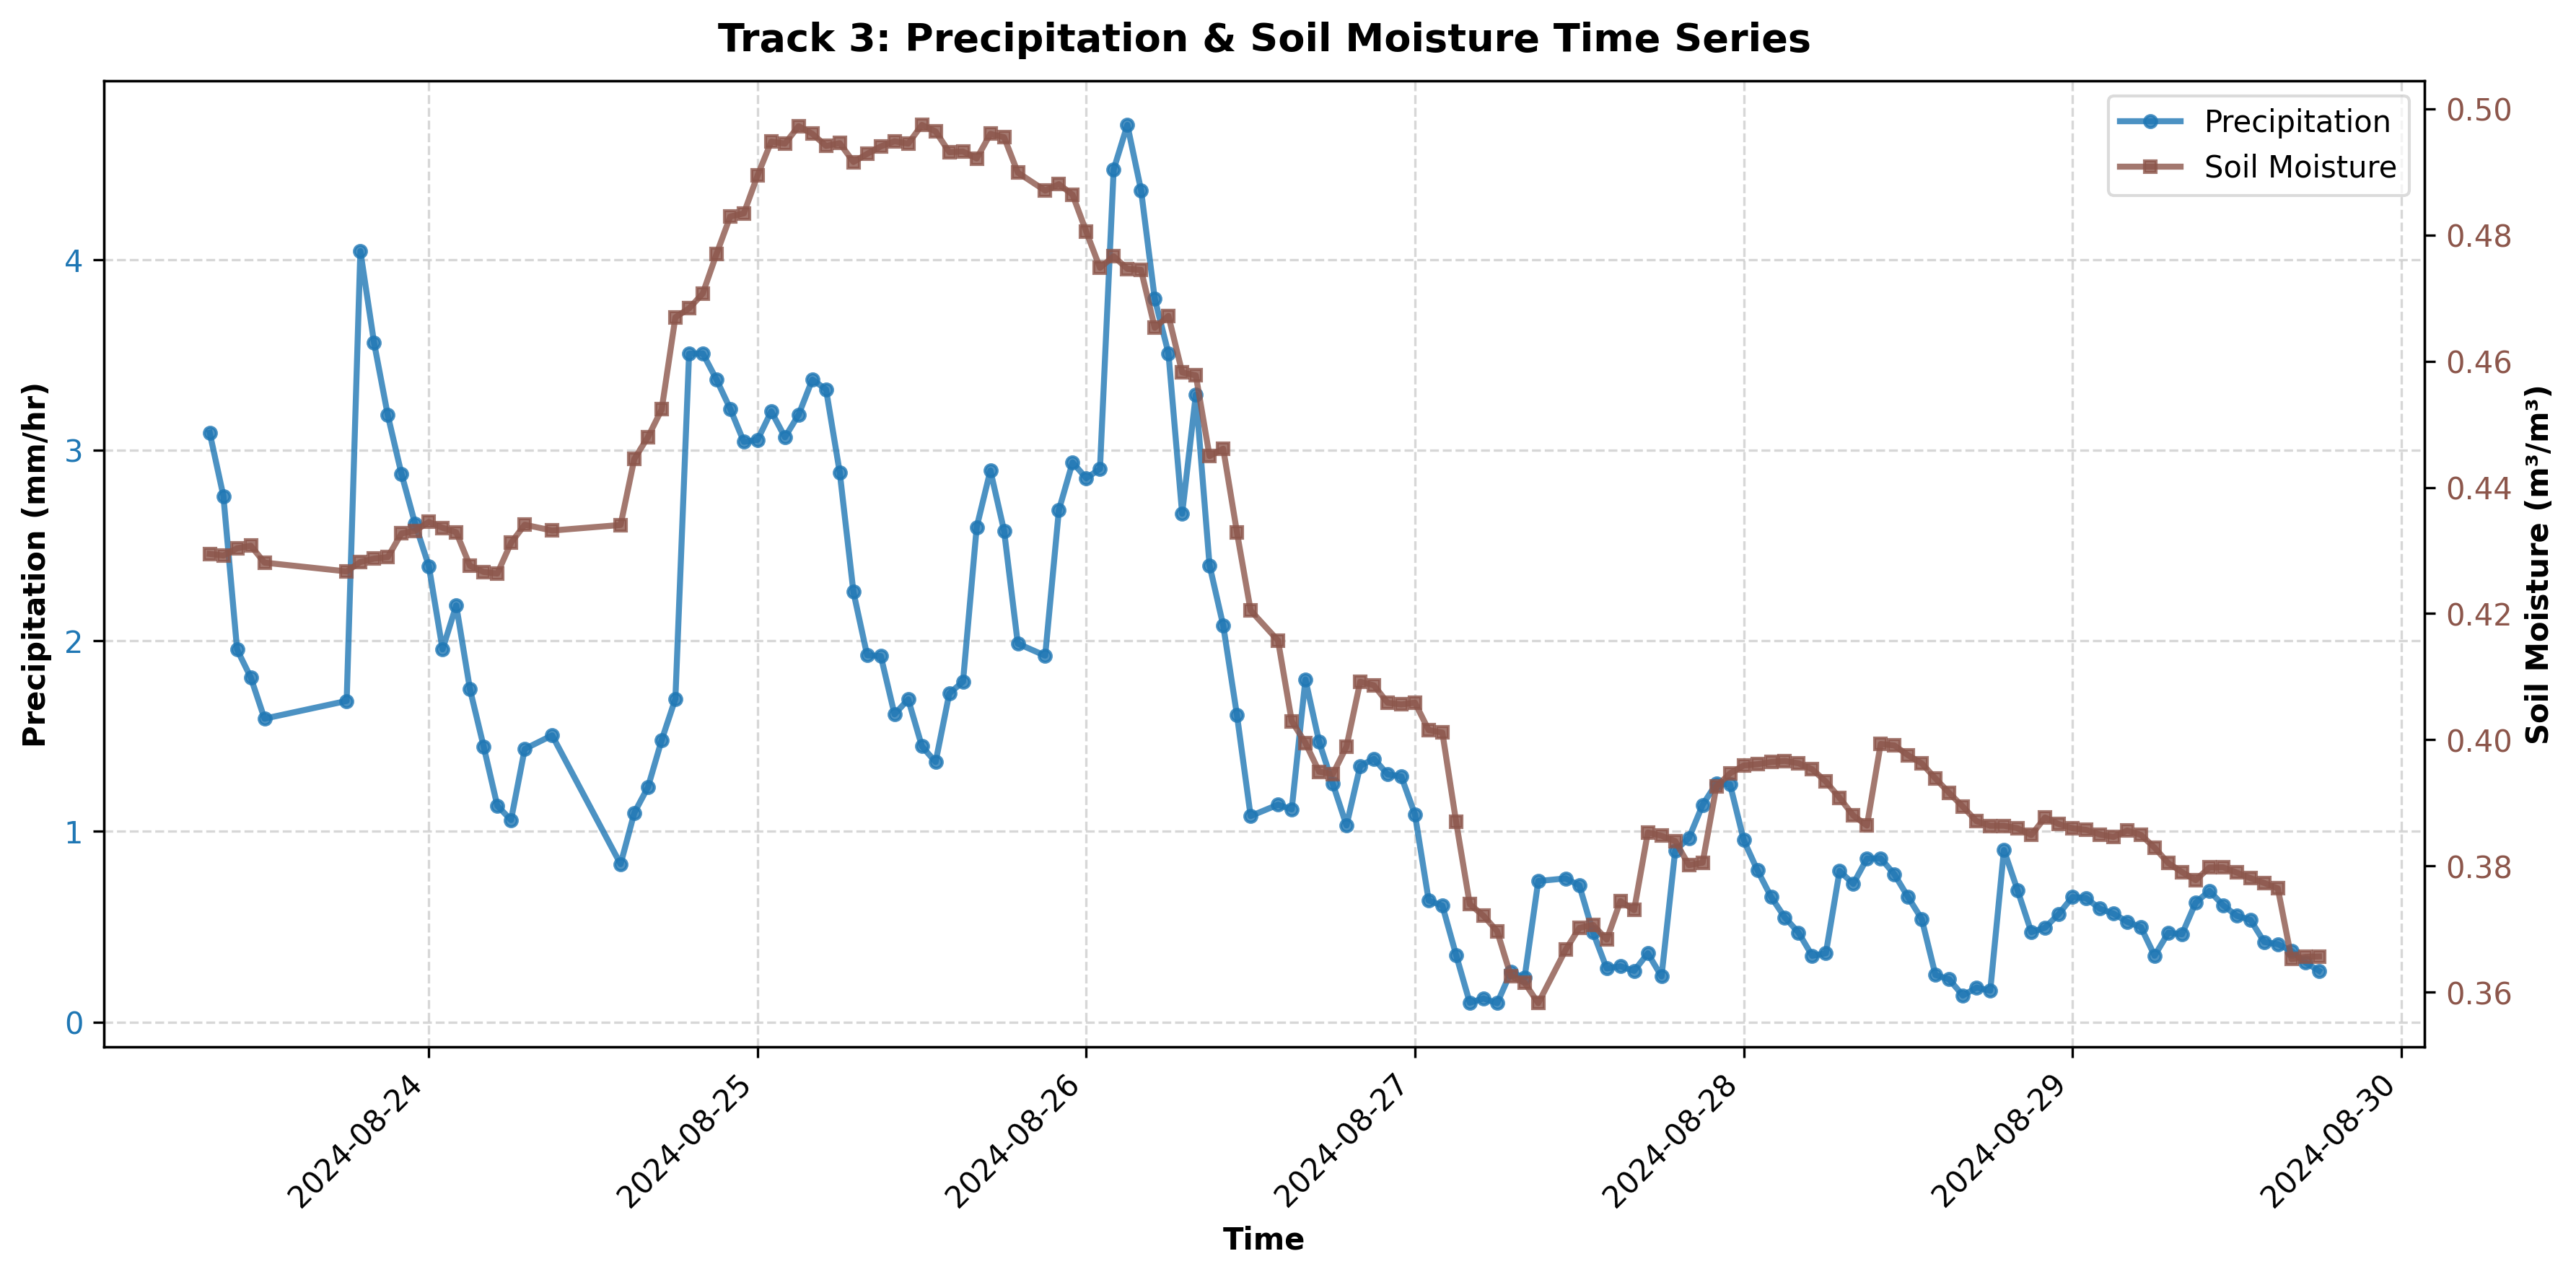
\includegraphics[width=0.7\textwidth]{../version5-with-no-ocean-masking/output/track_3/correlation_analysis/time_series/track_3_tp_sm_time_series.png}
	\end{center}
\end{frame}

% \begin{frame}{Track 3 Details - Heat fluxes transition}
% 	\begin{center}
% 		\includegraphics[width=0.8\textwidth]{../version5-with-no-ocean-masking/output/track_3/flux_analysis/track_3_analysis/track_3_heat_fluxes_trasnsition.png}
% 	\end{center}
% \end{frame}

\begin{frame}{Track 3 Details - Heat flux analysis}
	\begin{center}
		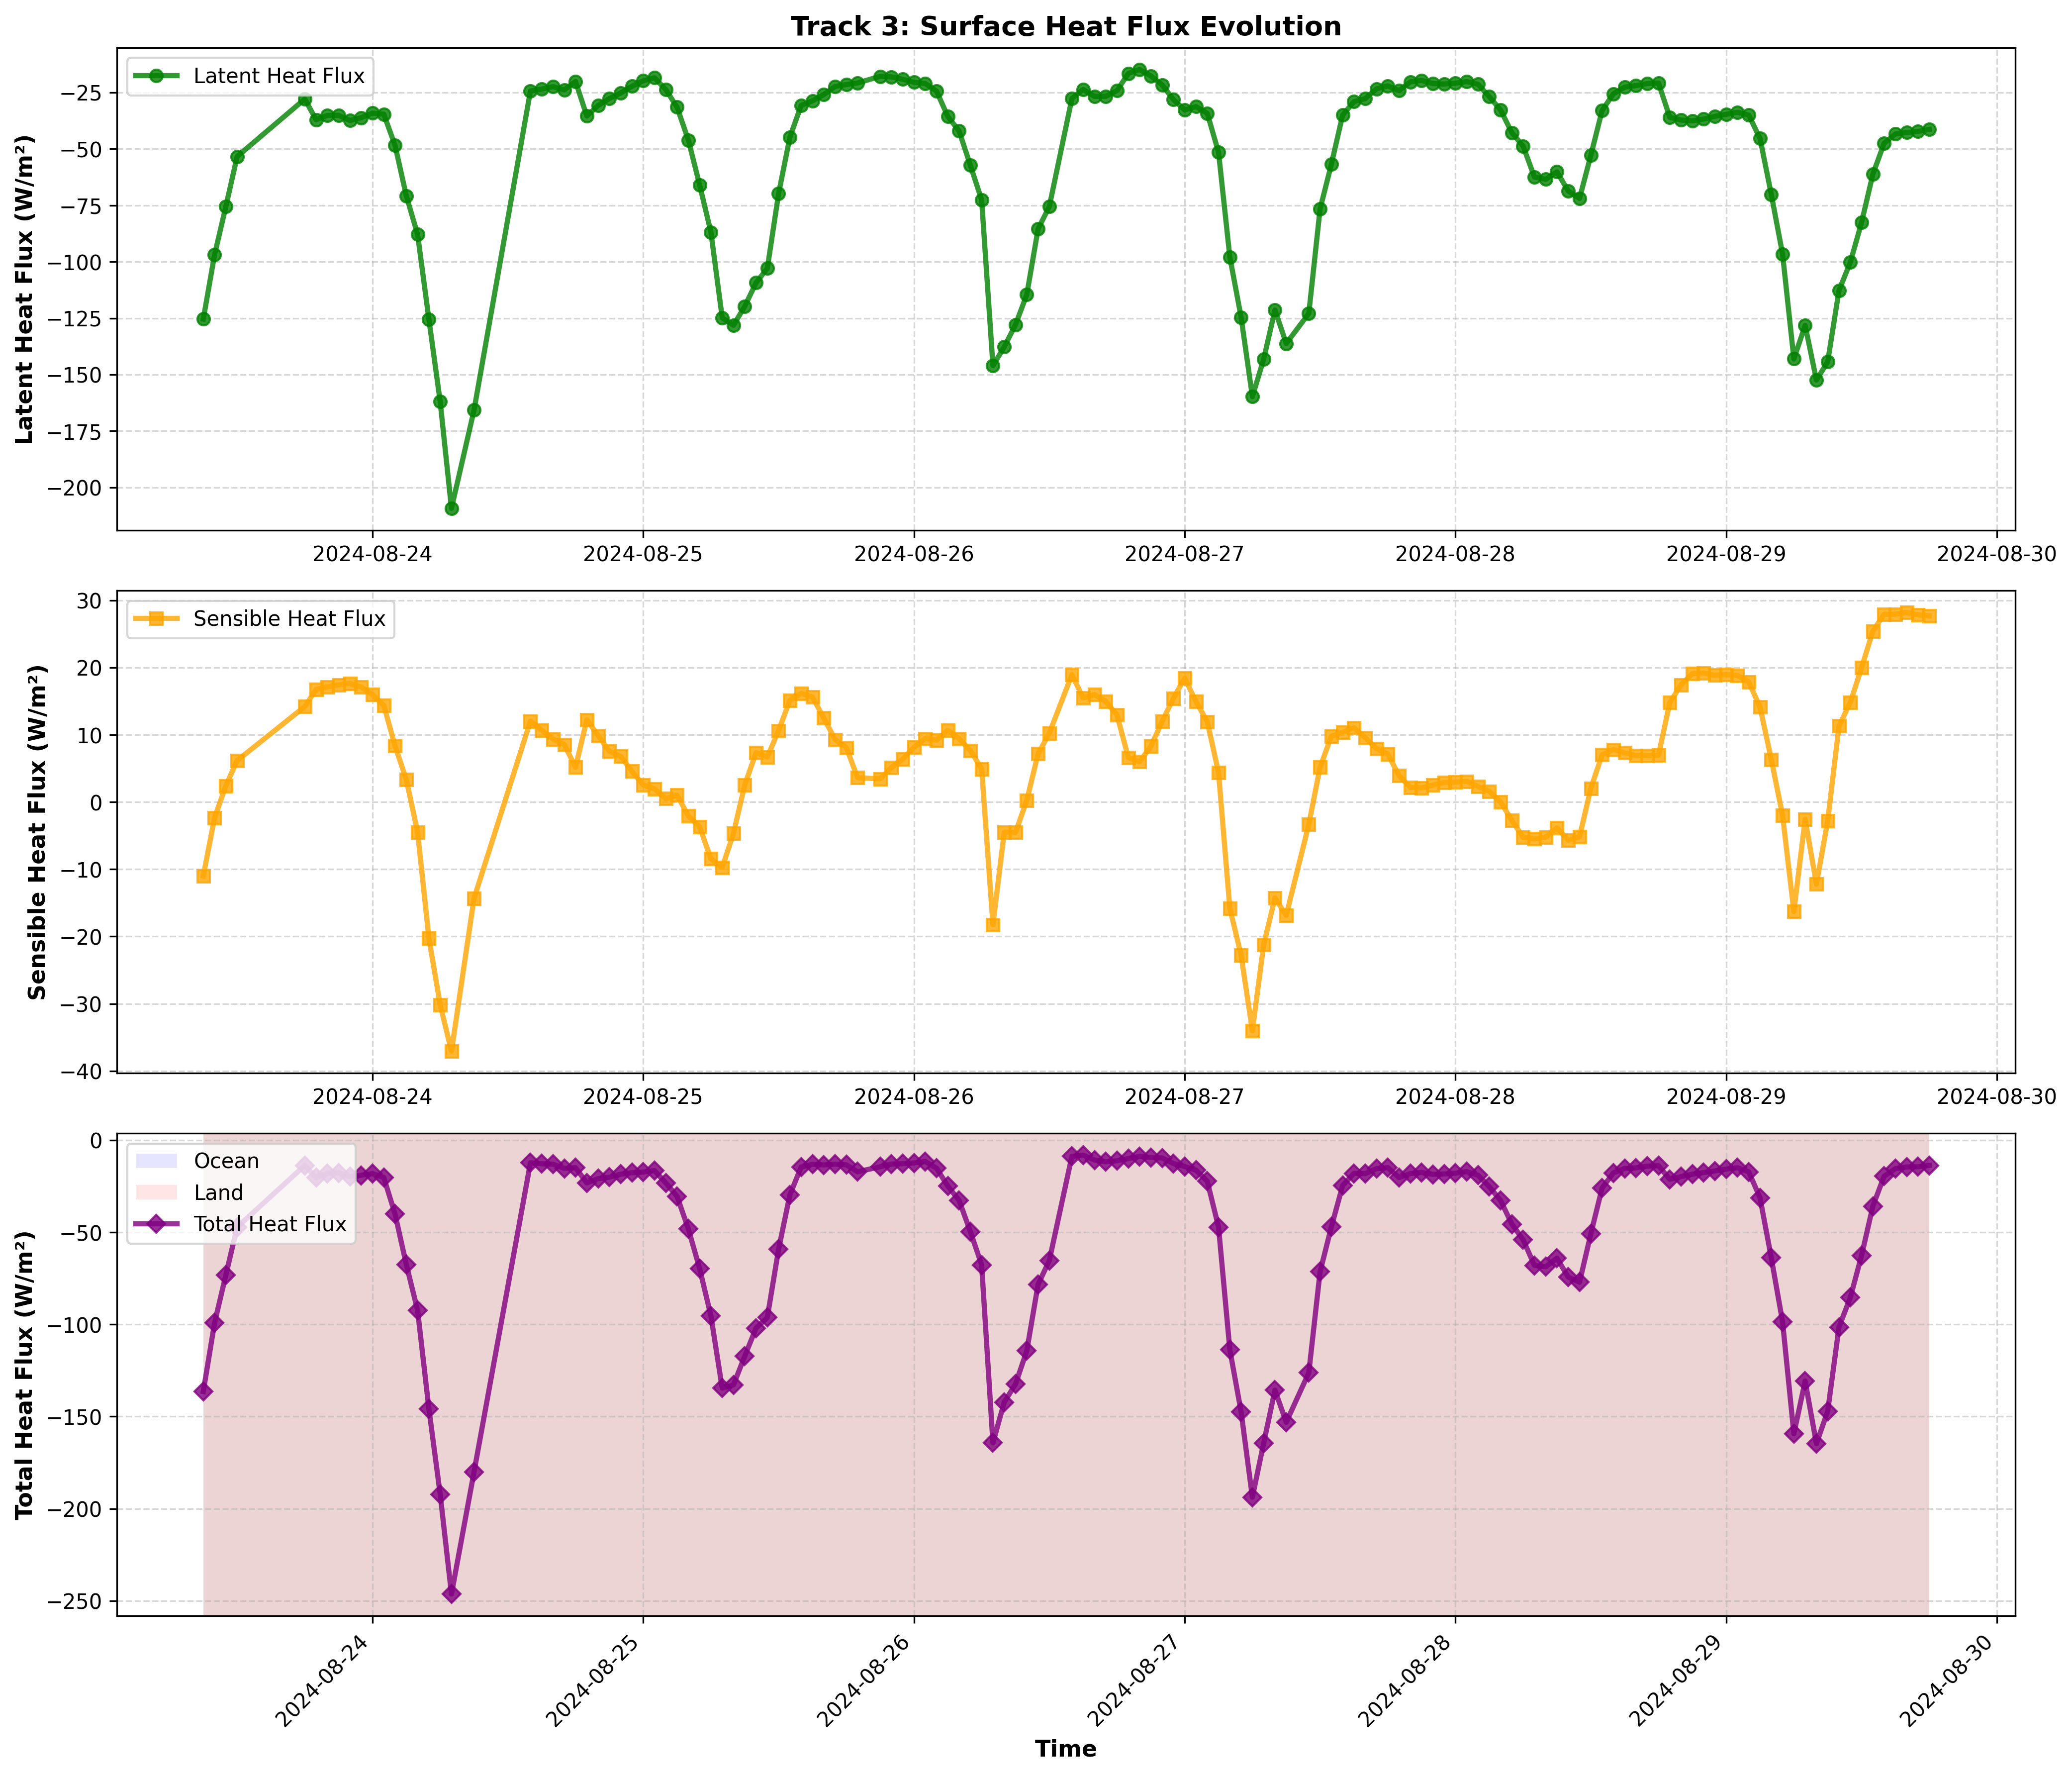
\includegraphics[width=0.6\textwidth]{../version5-with-no-ocean-masking/output/track_3/heat_flux_analysis/track_3_heat_flux_timeseries.png}
	\end{center}
\end{frame}

% %%%%%%%%%%%%%%%% Track 4 %%%%%%%%%%%%%%
\begin{frame}{Track 4 Details}
	\begin{center}
		\begin{columns}[T]
			\column{0.6\textwidth}
			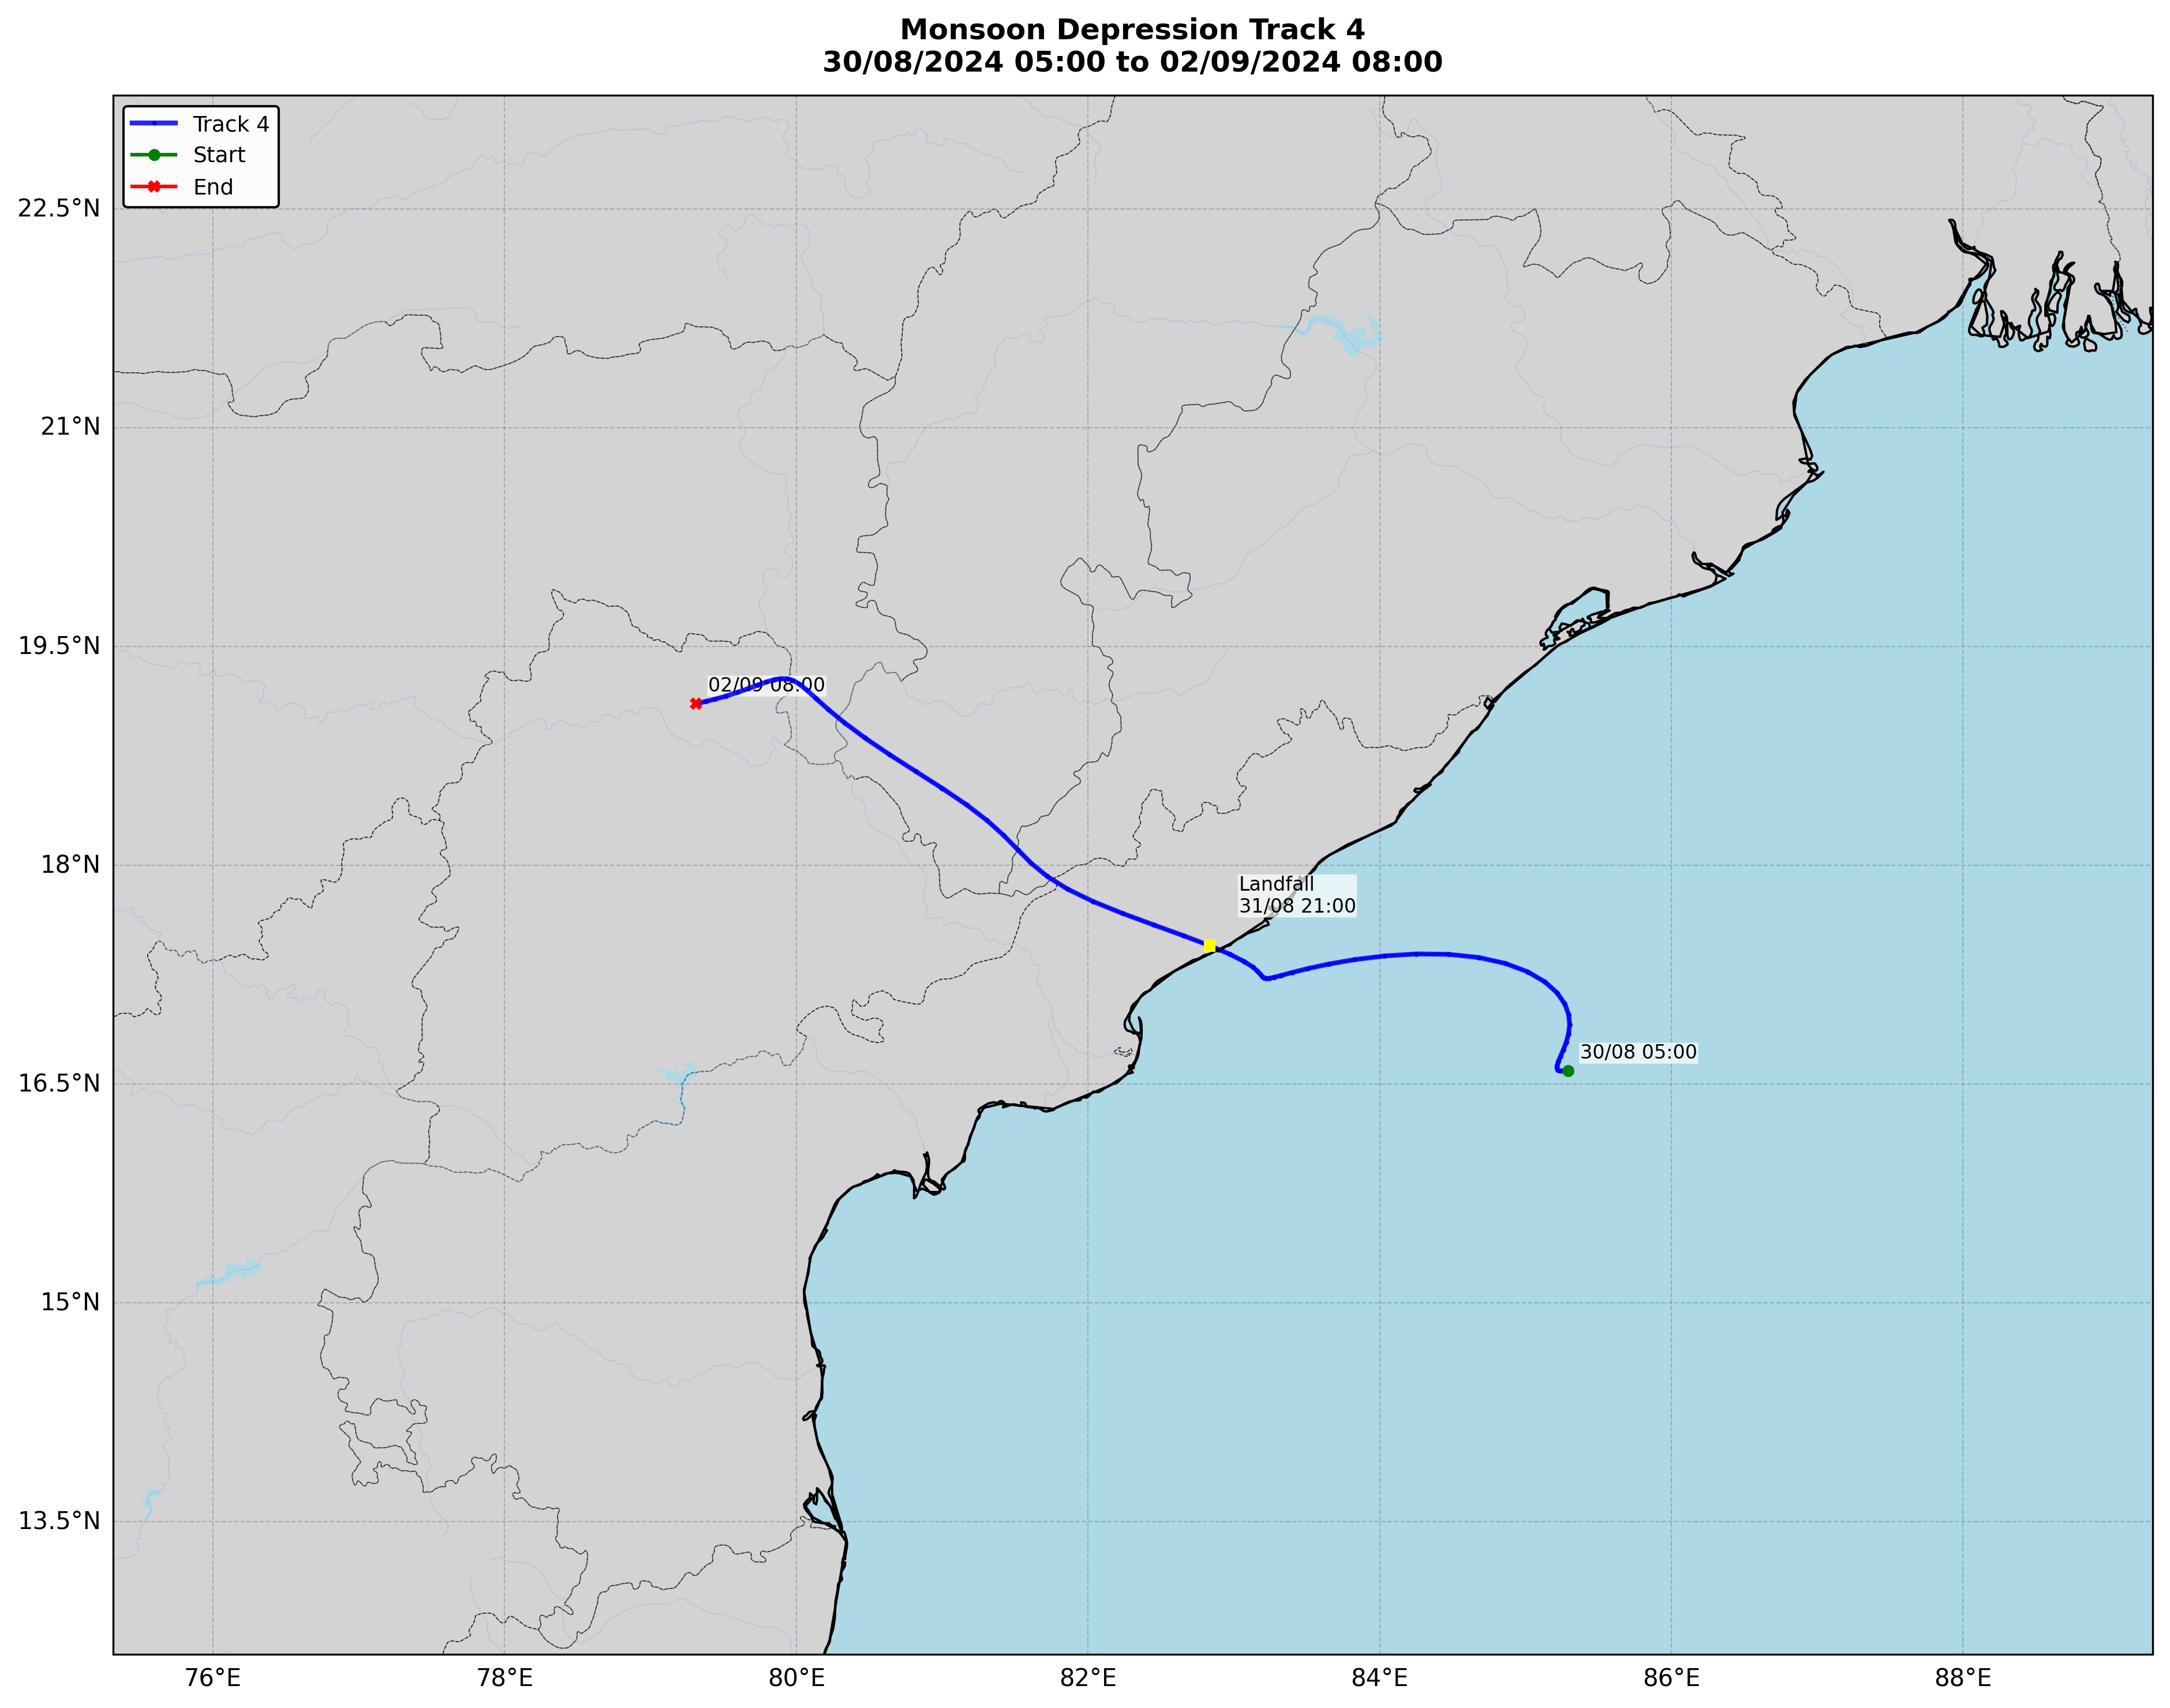
\includegraphics[width=0.95\textwidth]{../version5-with-no-ocean-masking/output/track_4/MD-track-4-detailed.png}

			\column{0.4\textwidth}
			\begin{block}{Statistics}
				\begin{itemize}
					\item Duration: 75 hours ($\sim$ 3 days)
					\item Category: short-lived MD
					\item Originated: over ocean
				\end{itemize}
			\end{block}
		\end{columns}
	\end{center}
\end{frame}

% 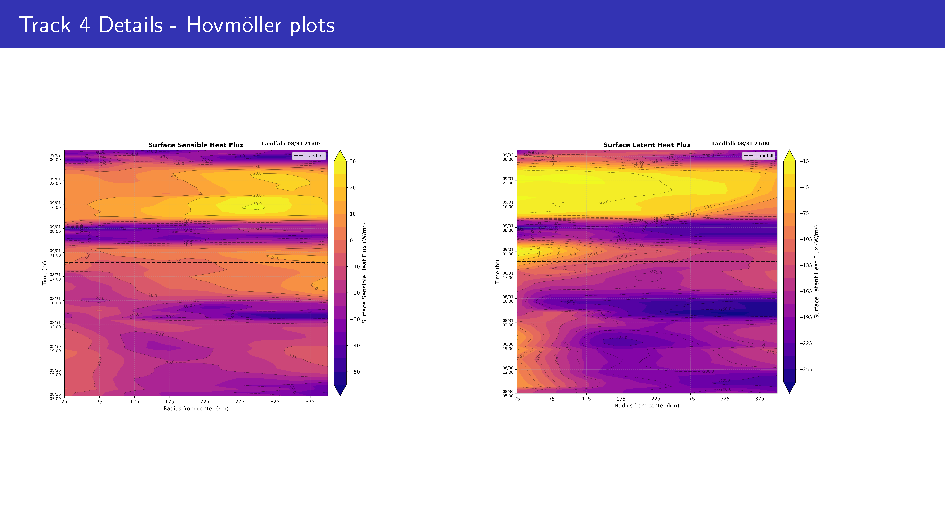
\includepdf[
% 	pages=-,
% 	scale=1,
% 	frame=true,
% 	pagecommand={\thispagestyle{empty}},  % Remove page numbers
% 	offset=0mm 0mm,       % Adjust position
% 	% templatesize={\textwidth}{\textheight} % Match template size
% ]{hovmoller-slides/hov-4.pdf}

% \begin{frame}{Track 4 Details - Precipitation and soil moisture over time along track}
% 	\begin{center}
% 		\includegraphics[width=0.8\textwidth]{../version5-with-no-ocean-masking/output/track_4/correlation_analysis/time_series/track_4_time_series.png}
% 	\end{center}
% \end{frame}

\begin{frame}{Track 4 Details - Translation speed of MD}
	\begin{center}
		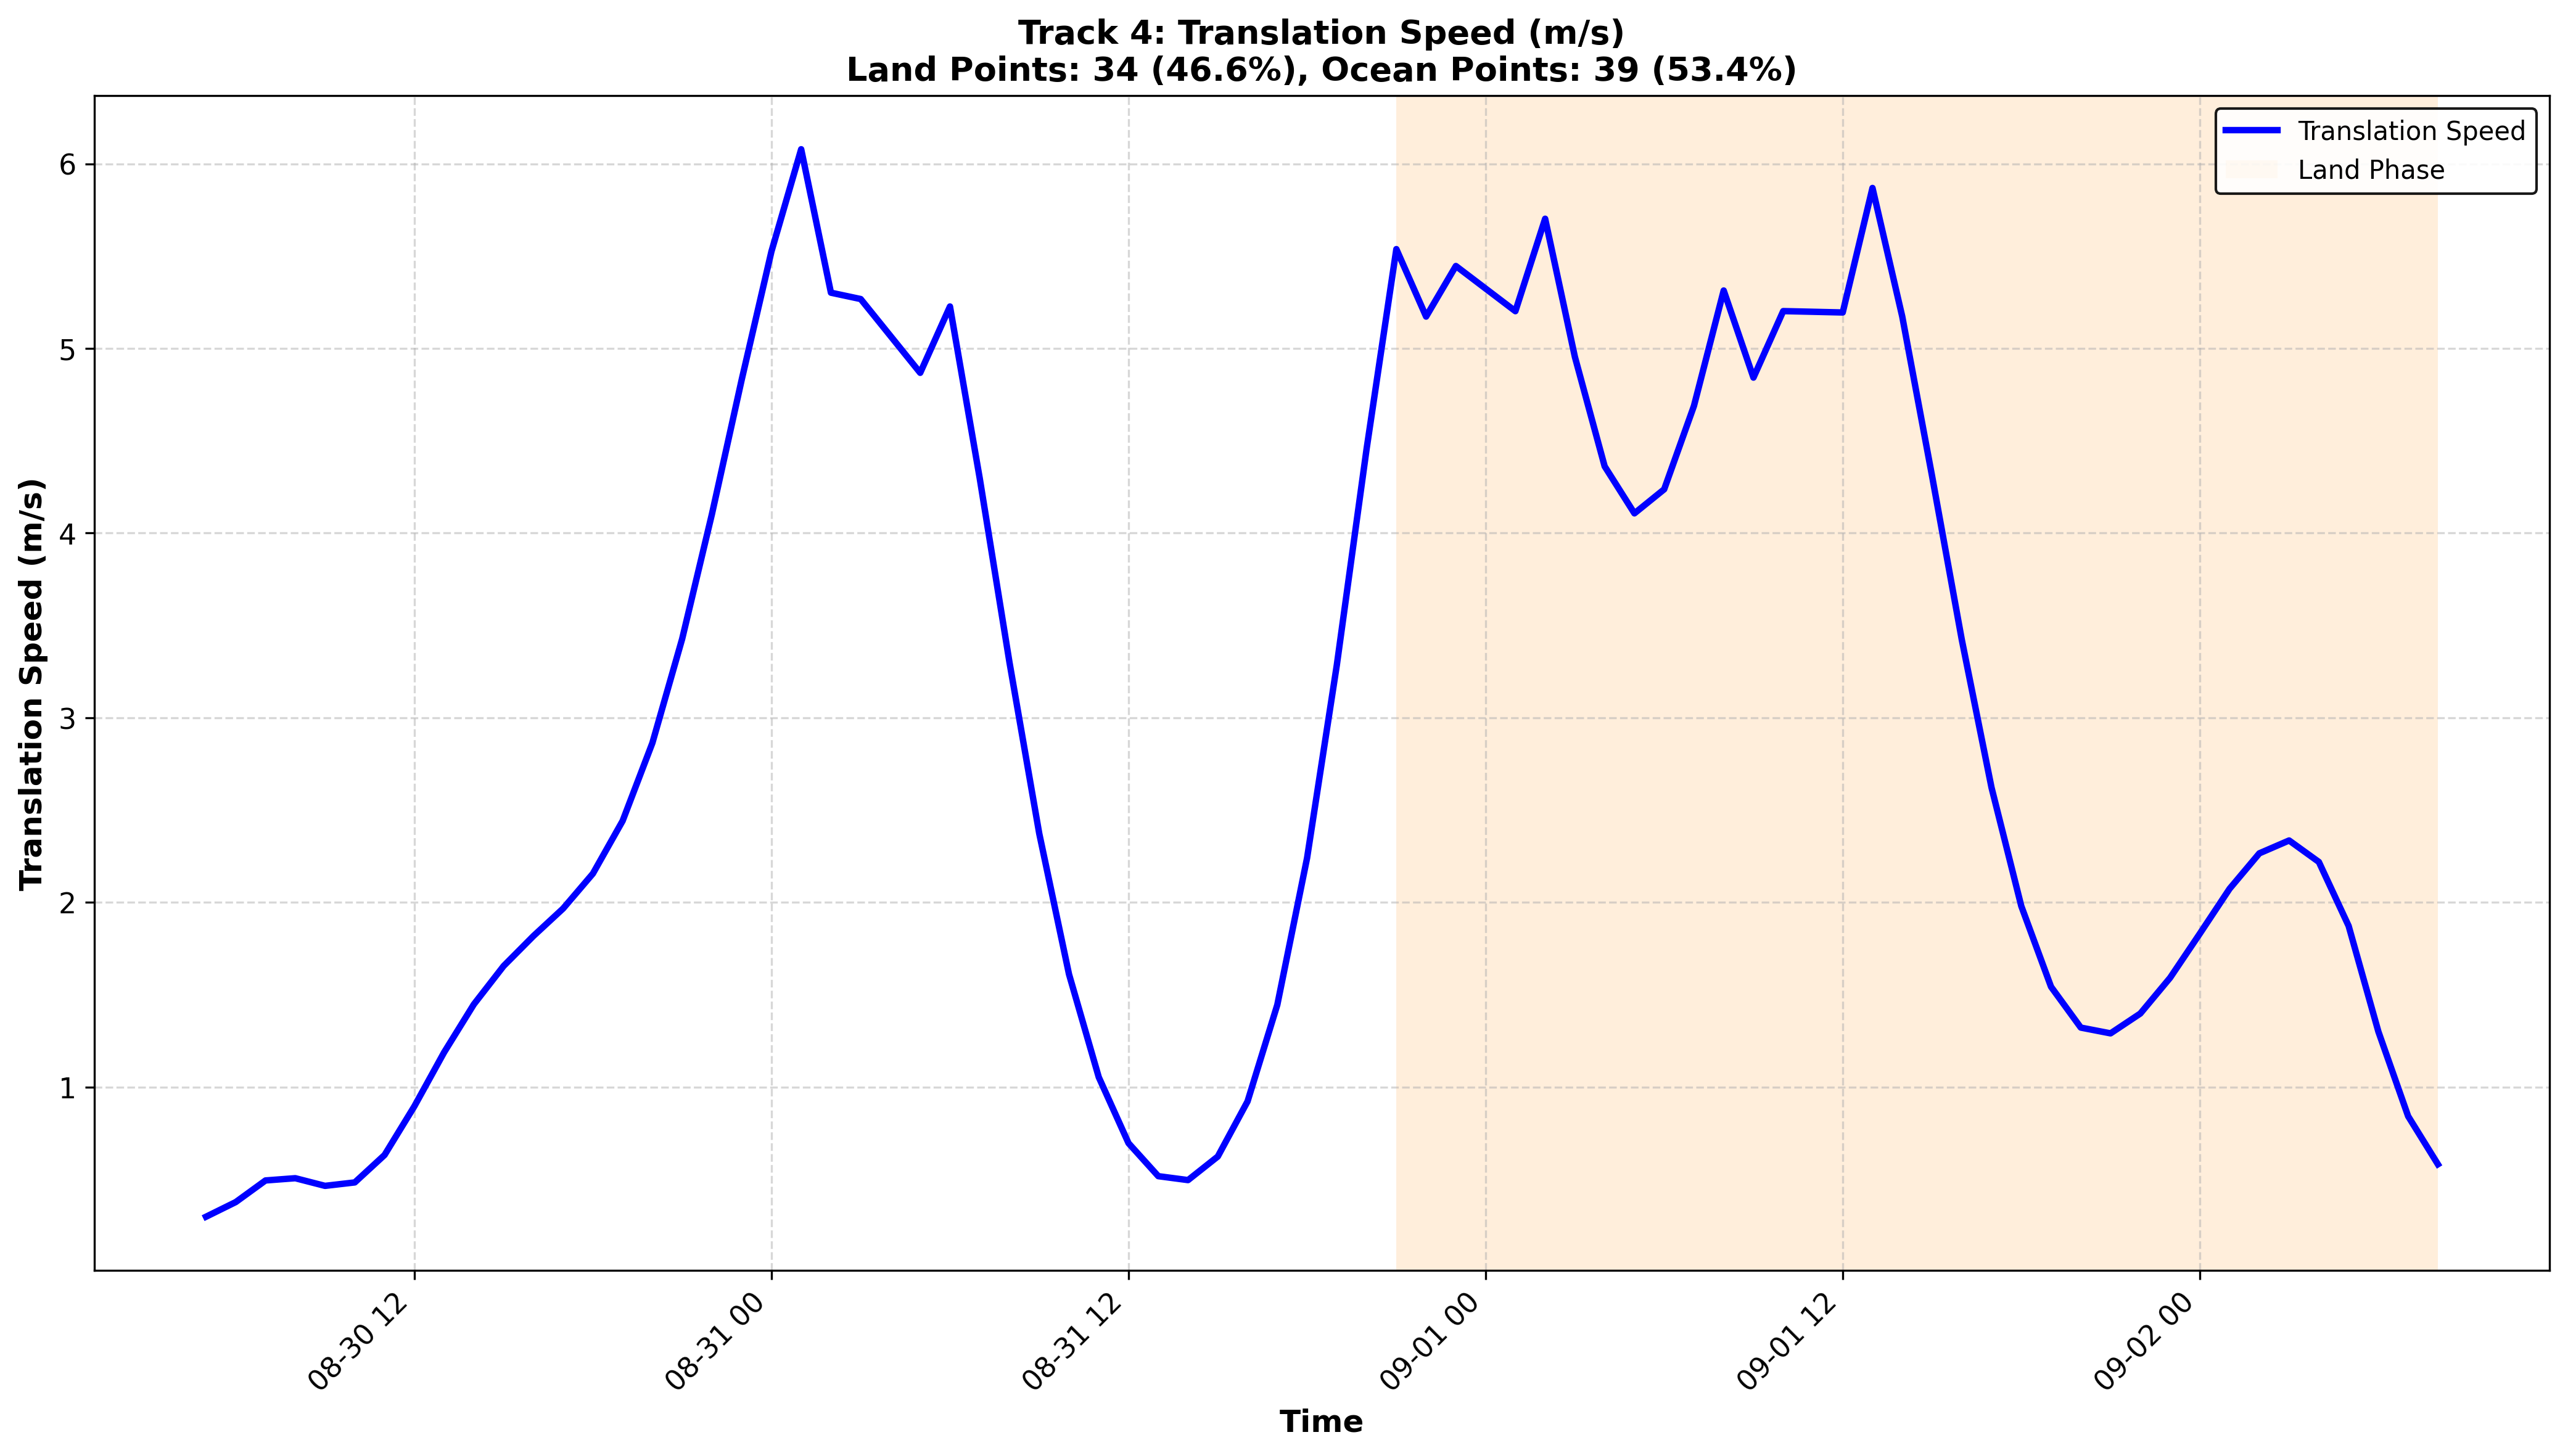
\includegraphics[width=0.8\textwidth]{../version5-with-no-ocean-masking/output/track_4/translational-speed/track_4_speed_ms.png}
	\end{center}
\end{frame}

\begin{frame}{Track 4 Details - Lag Correlation}
	\begin{center}
		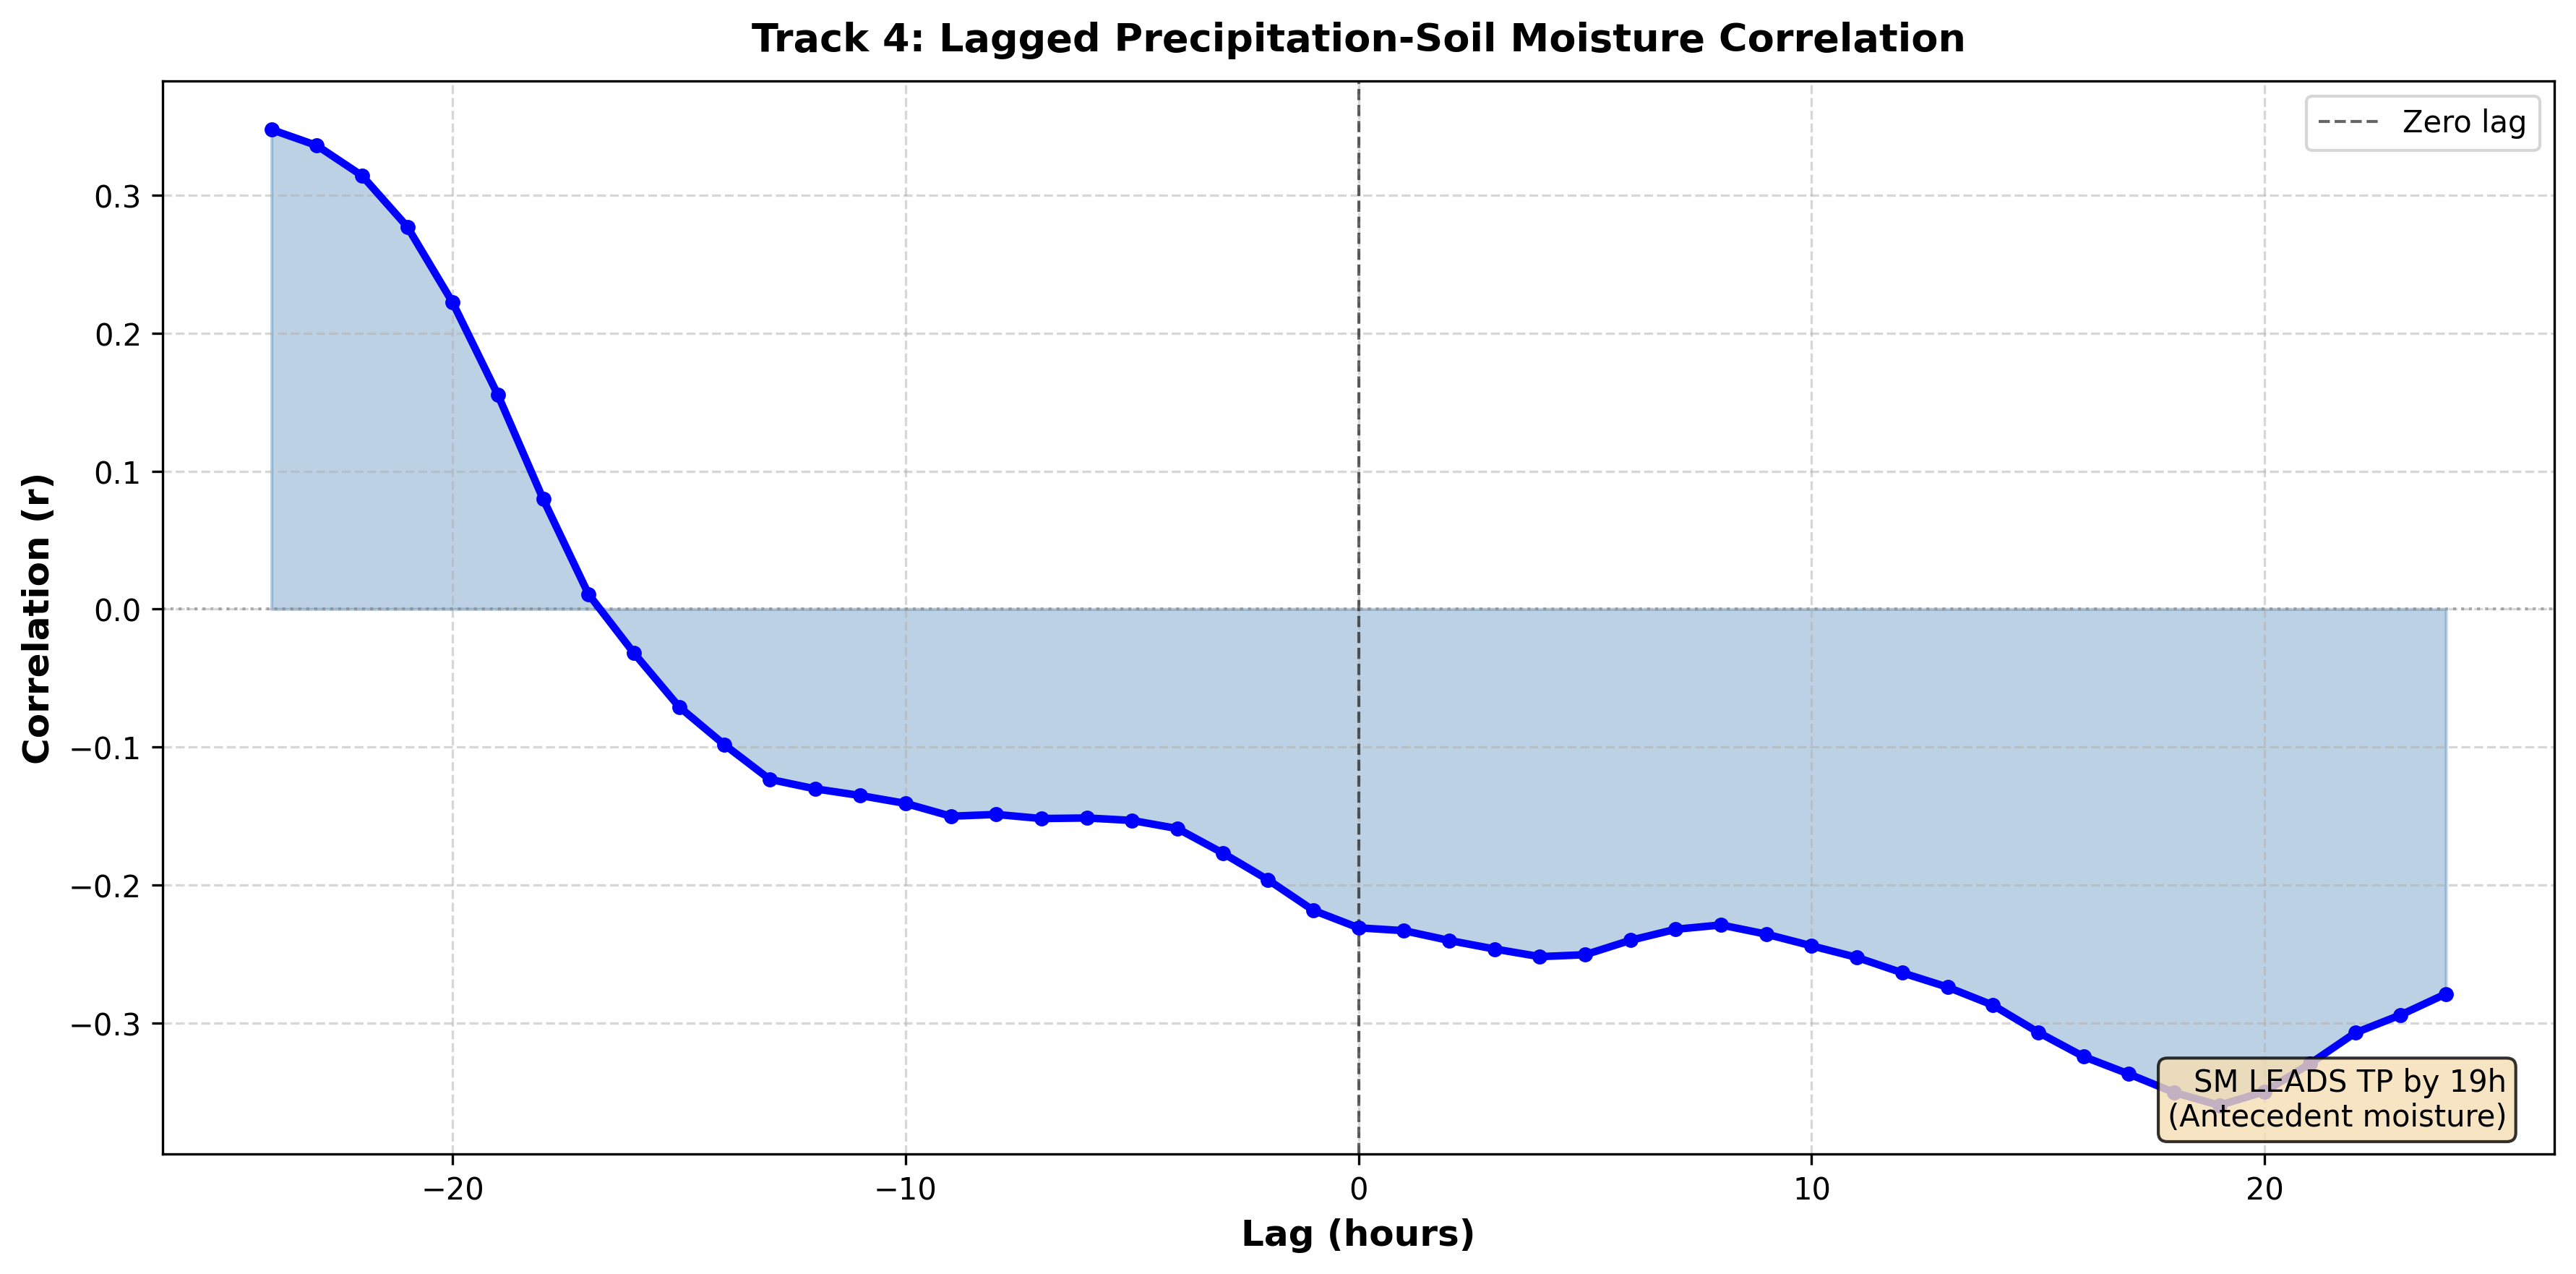
\includegraphics[width=0.8\textwidth]{../version5-with-no-ocean-masking/output/track_4/correlation_analysis/lag_correlation/track_4_lag_corr.png}
	\end{center}
\end{frame}

\begin{frame}{Track 4 Details - TP - SWVL1 Correlation}
	\begin{center}
		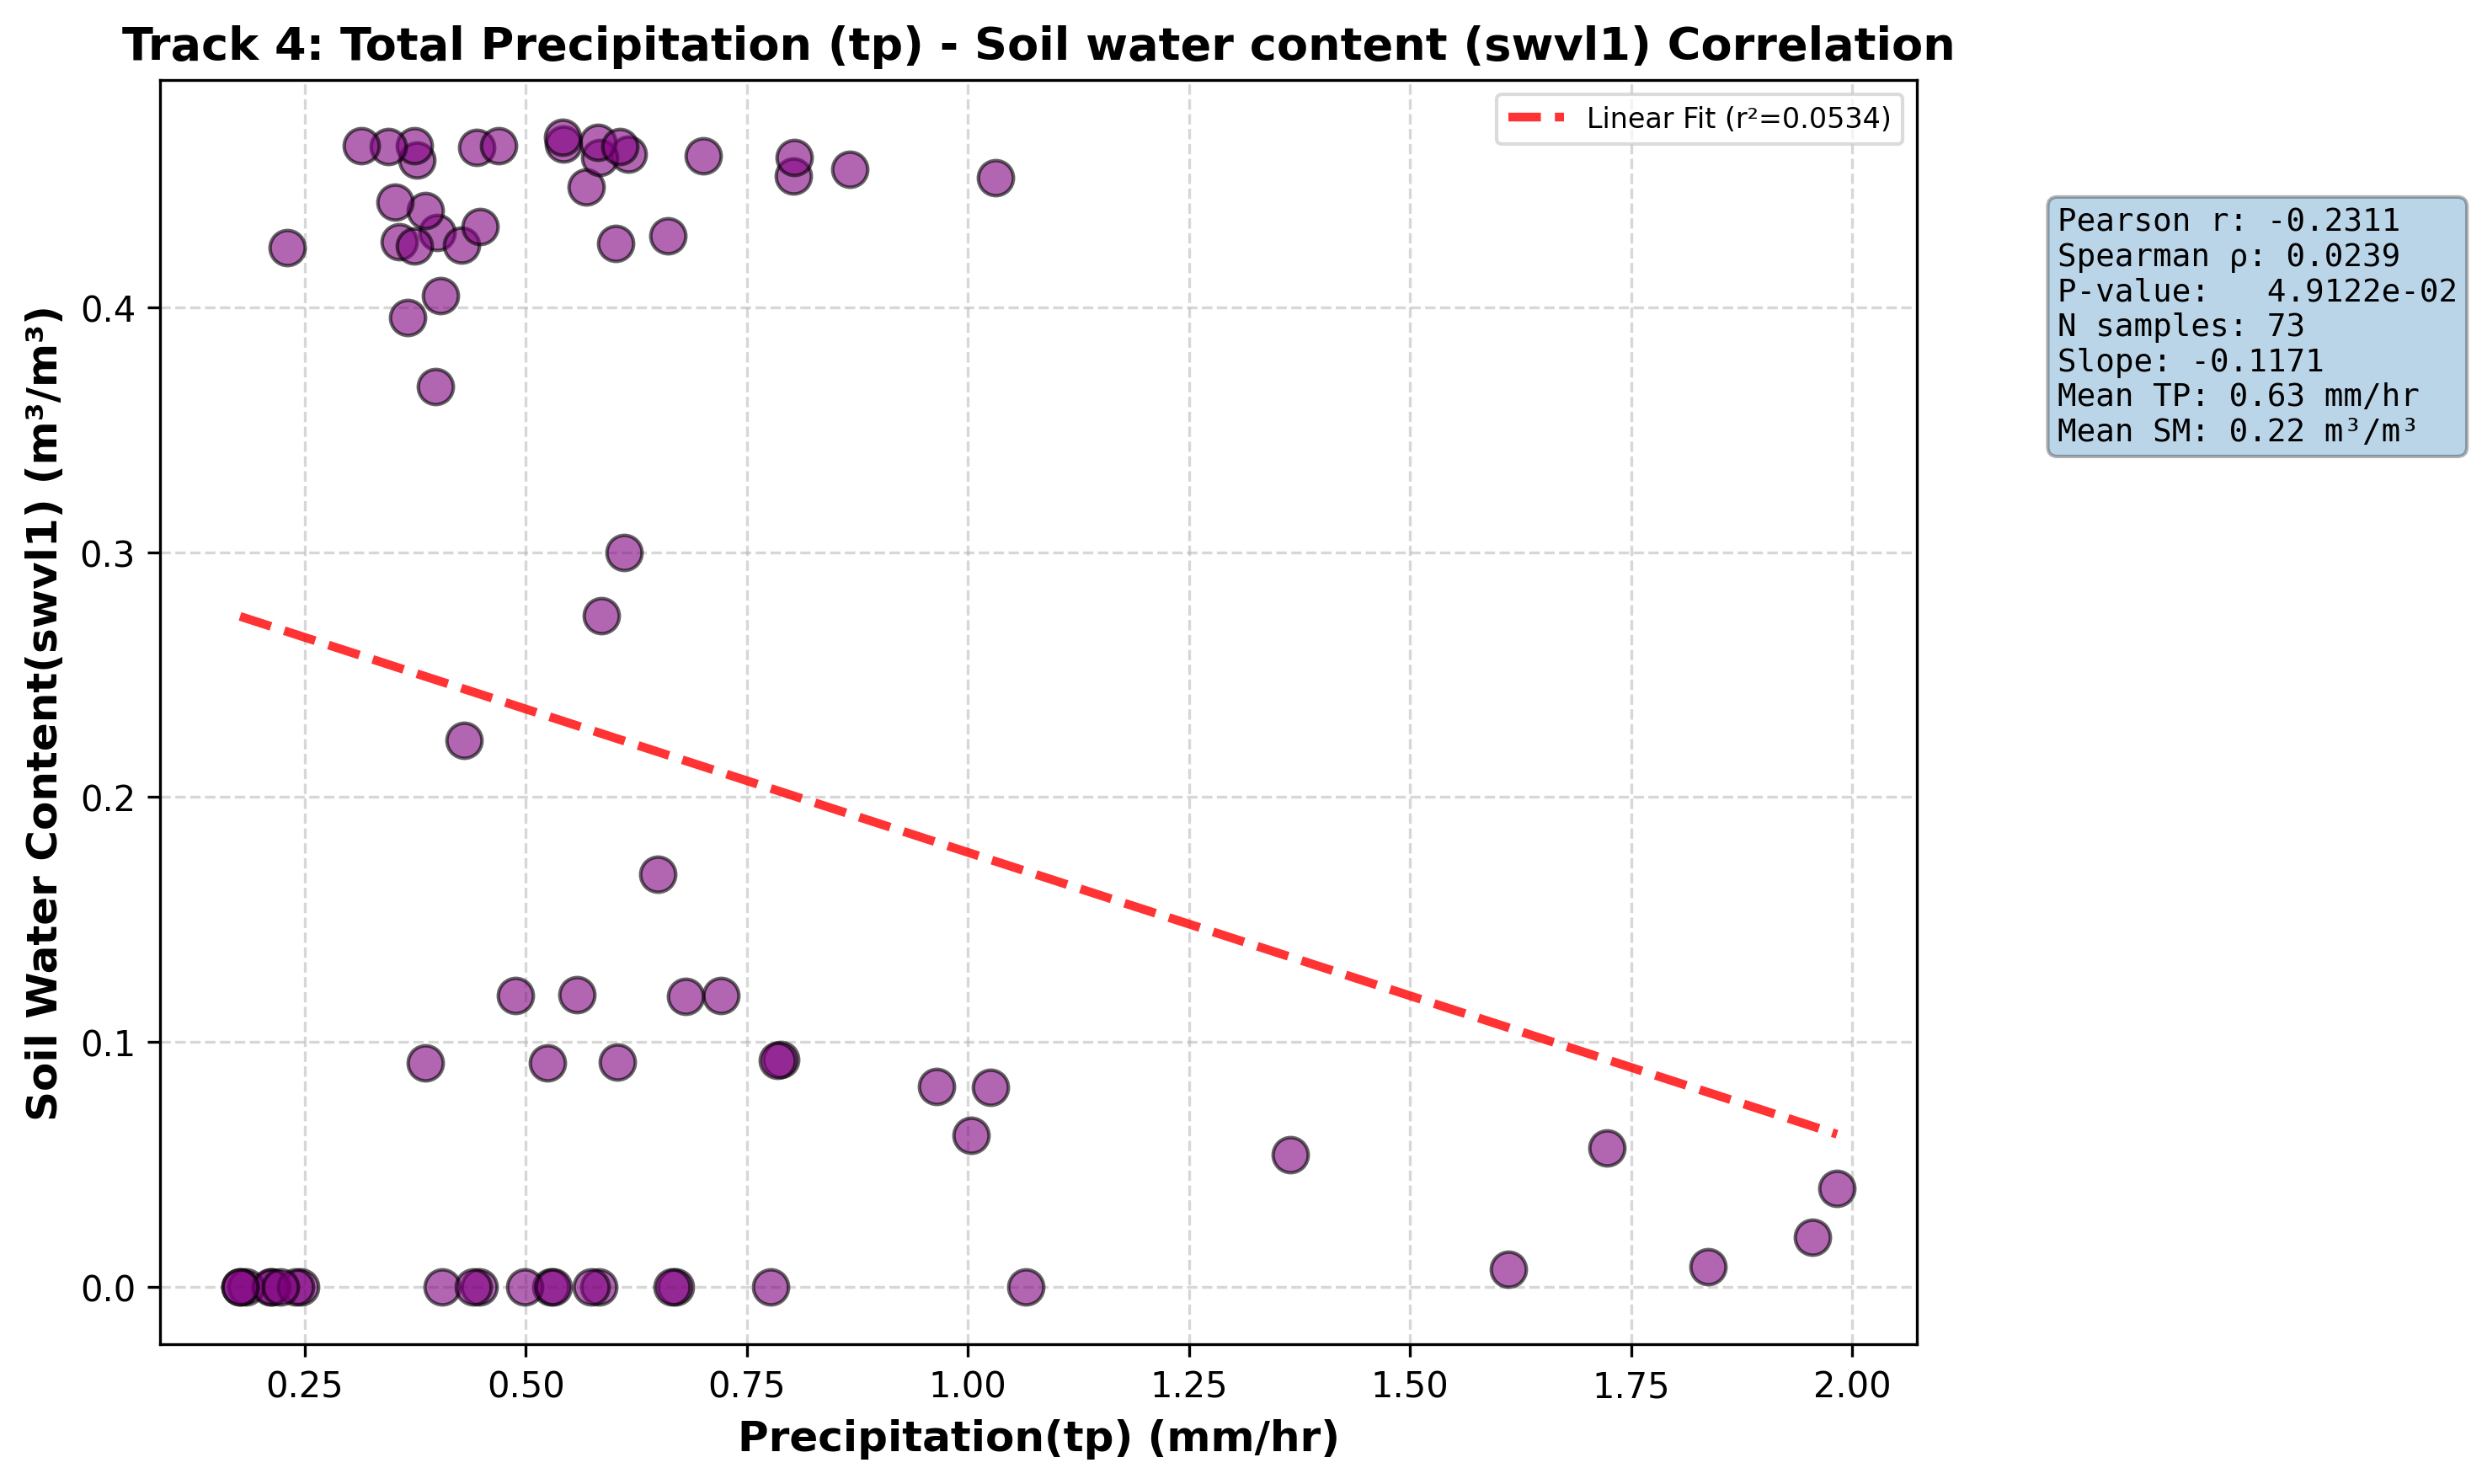
\includegraphics[width=0.7\textwidth]{../version5-with-no-ocean-masking/output/track_4/correlation_analysis/scatter_plots/track_4_scatter.png}
	\end{center}
\end{frame}

\begin{frame}{Track 4 Details - Spatial distribution of TP and SWVL1}
	\begin{center}
		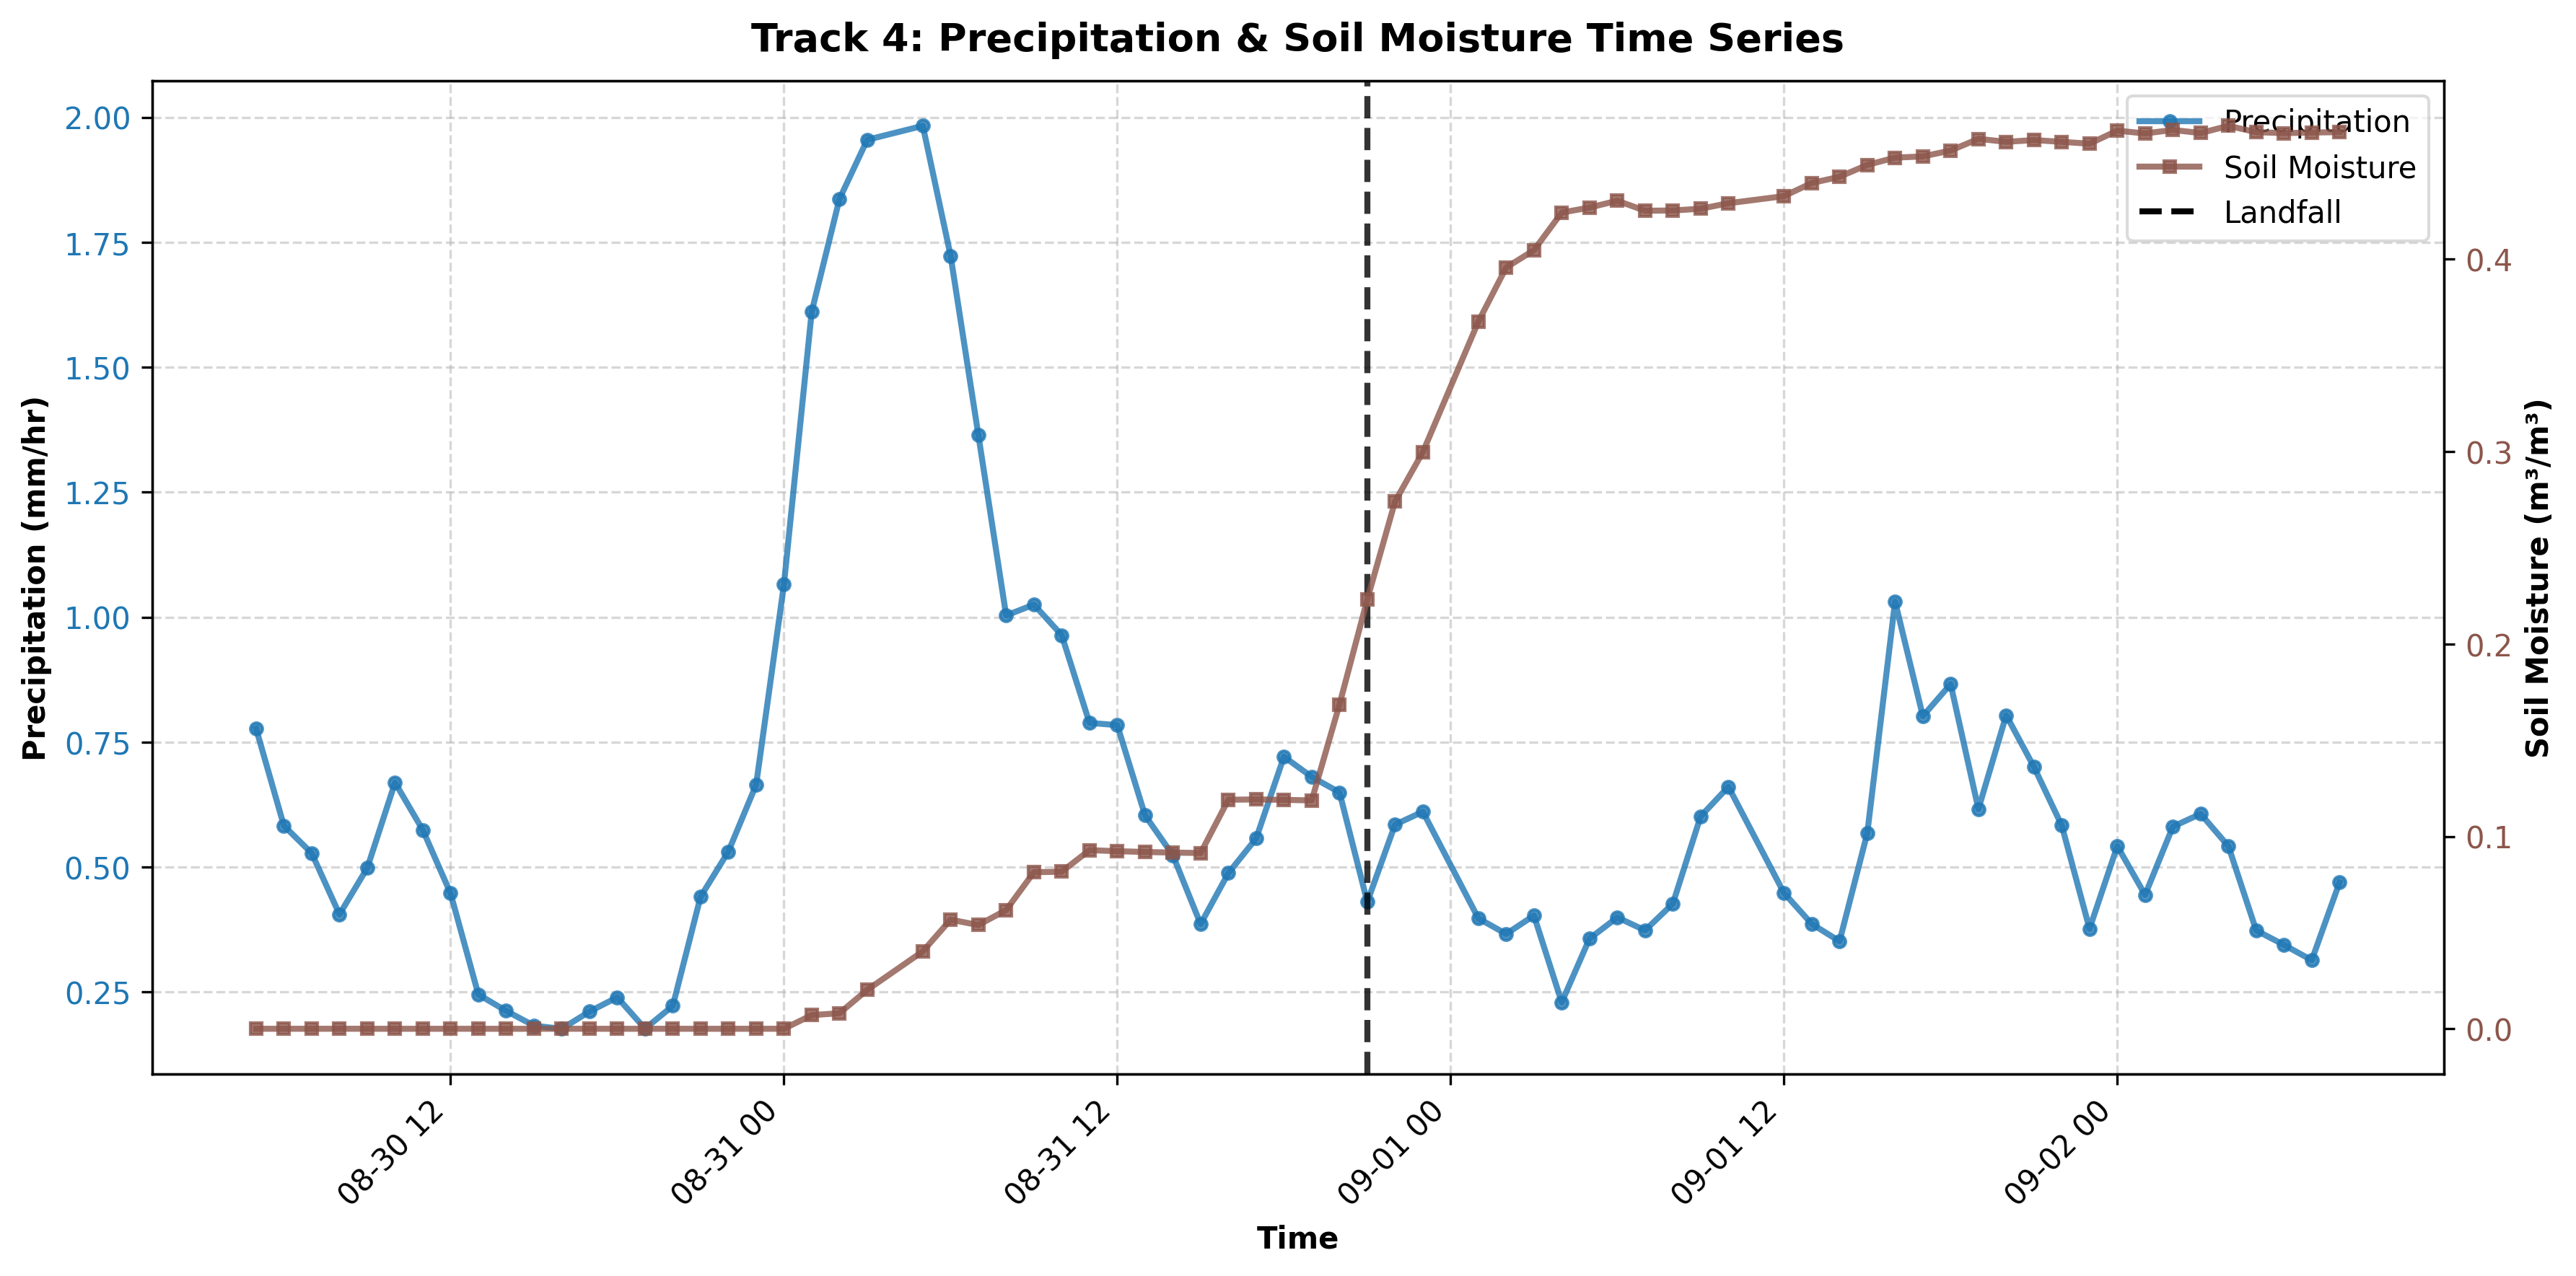
\includegraphics[width=0.7\textwidth]{../version5-with-no-ocean-masking/output/track_4/correlation_analysis/time_series/track_4_tp_sm_time_series.png}
	\end{center}
\end{frame}

% \begin{frame}{Track 4 Details - Heat fluxes transition}
% 	\begin{center}
% 		\includegraphics[width=0.8\textwidth]{../version5-with-no-ocean-masking/output/track_4/flux_analysis/track_4_analysis/track_4_heat_fluxes_trasnsition.png}
% 	\end{center}
% \end{frame}

\begin{frame}{Track 4 Details - Heat flux analysis}
	\begin{center}
		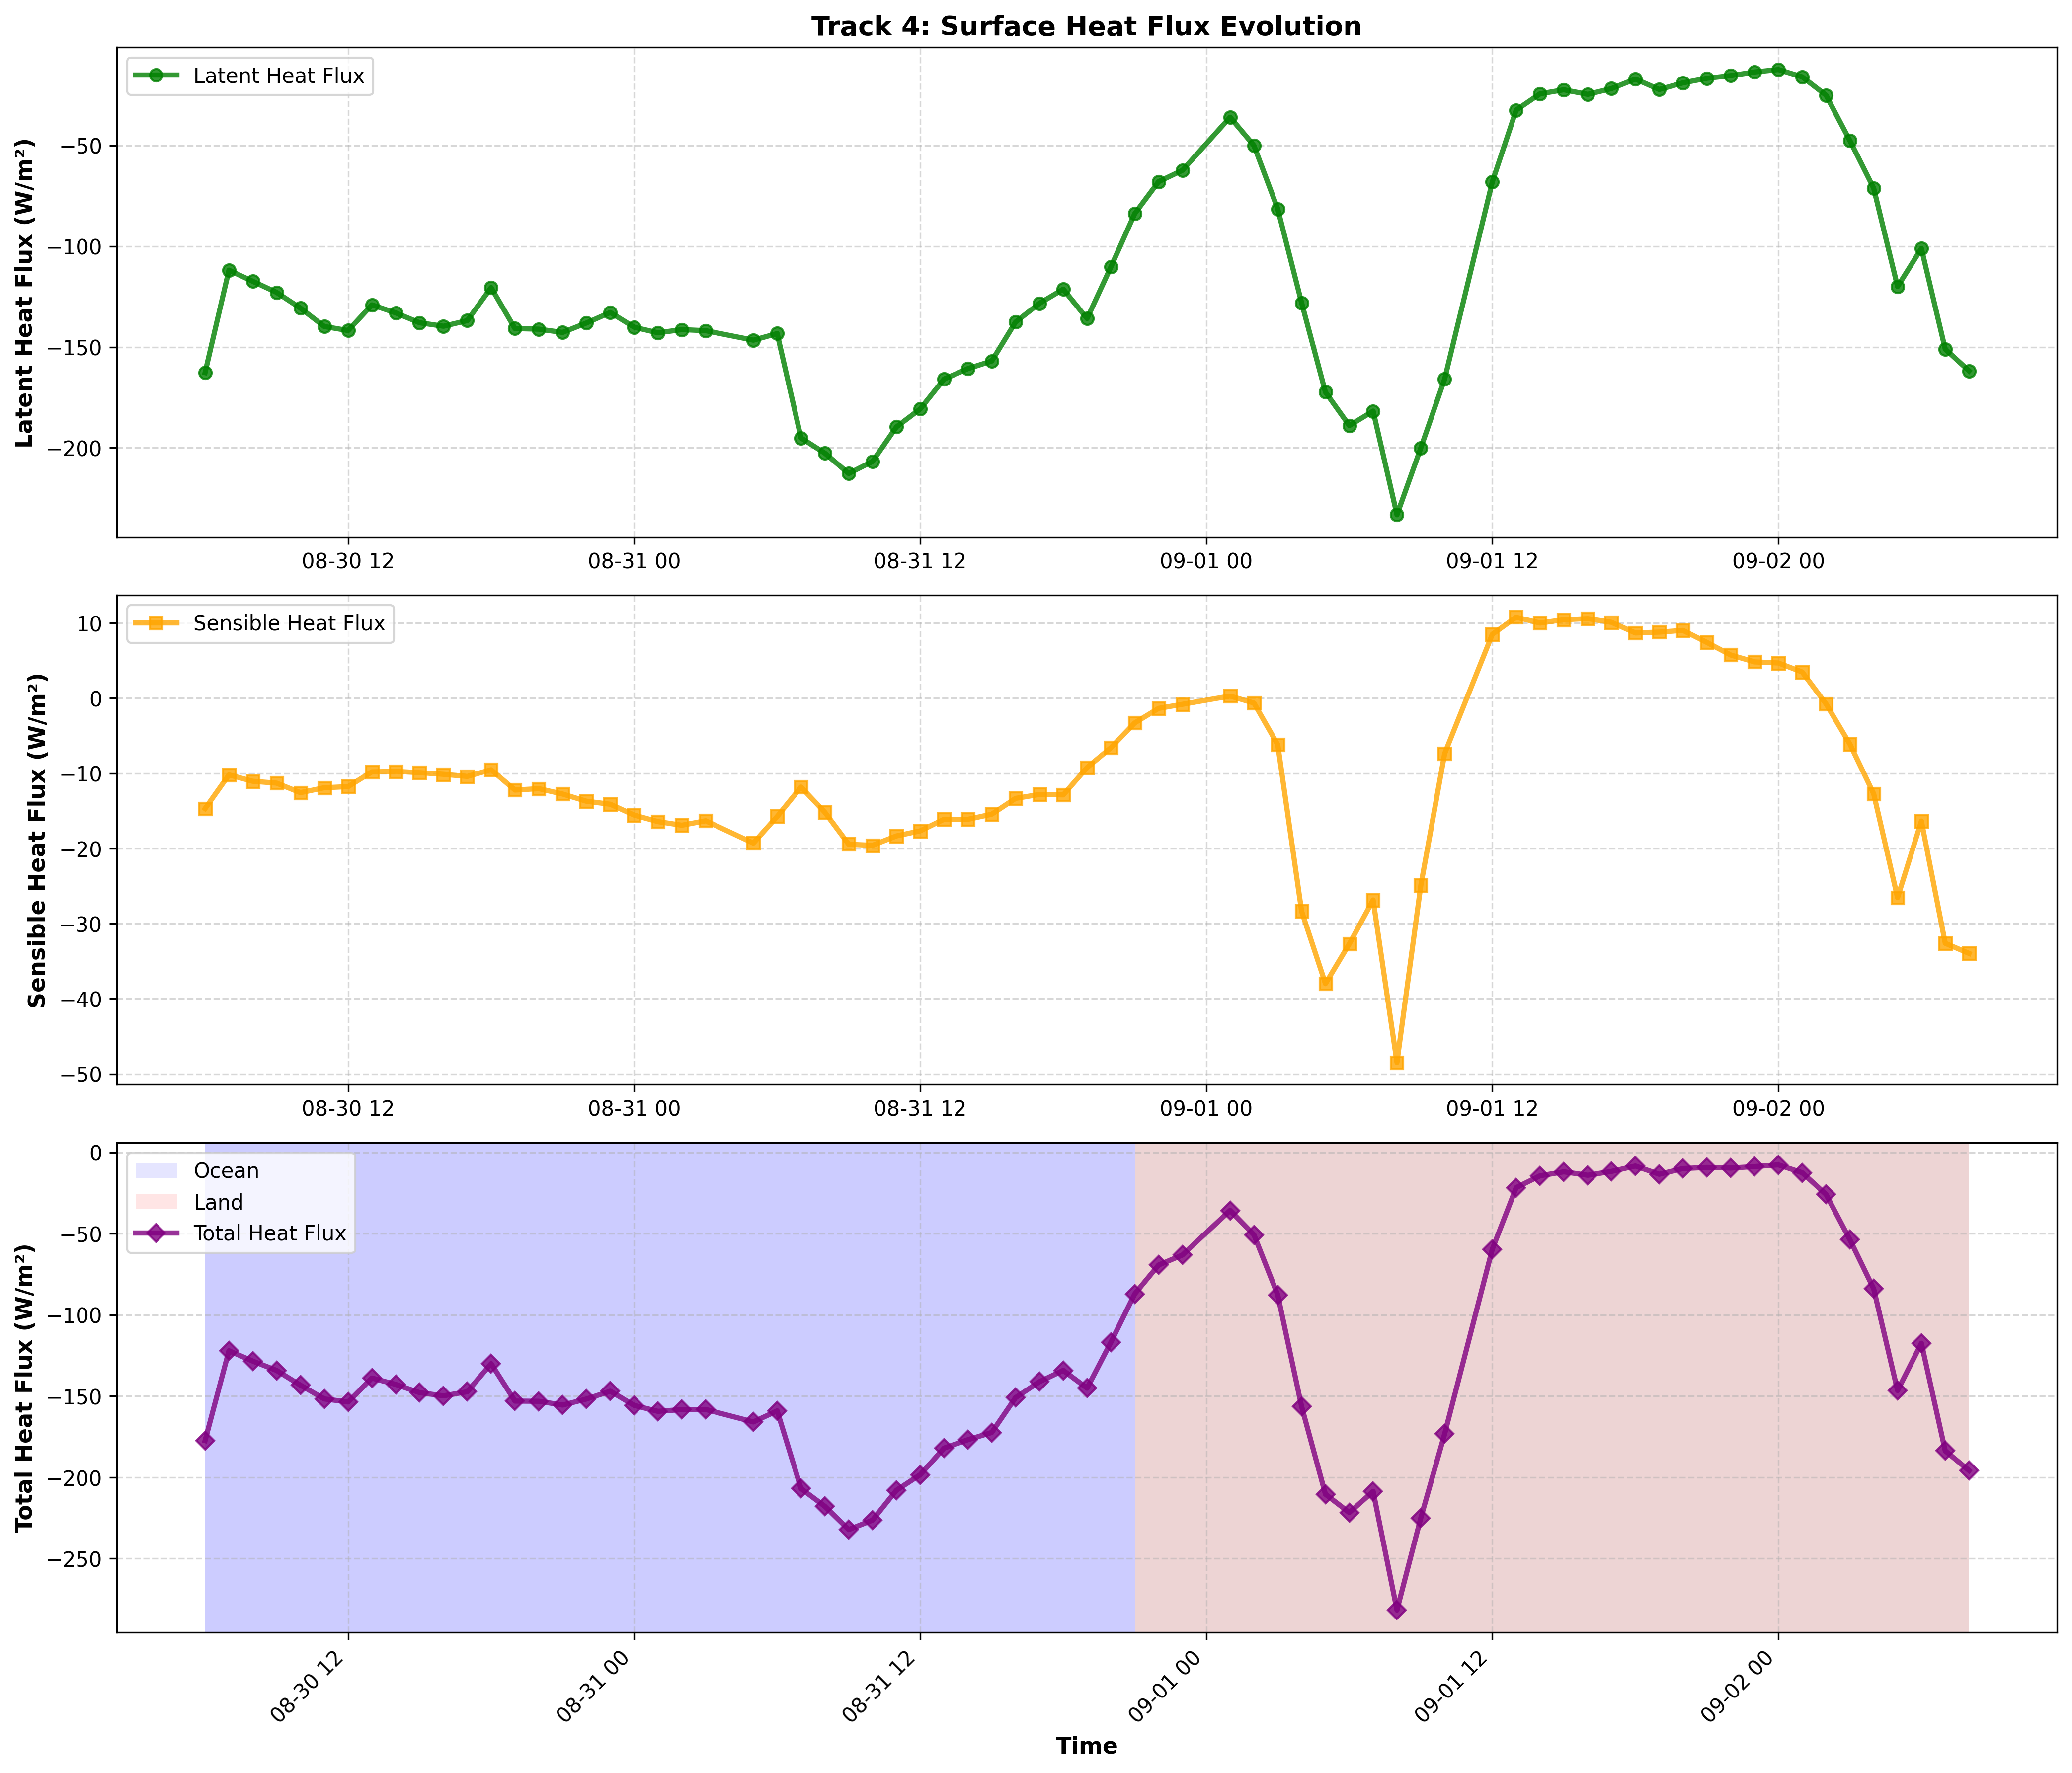
\includegraphics[width=0.6\textwidth]{../version5-with-no-ocean-masking/output/track_4/heat_flux_analysis/track_4_heat_flux_timeseries.png}
	\end{center}
\end{frame}


% %%%%%%%%%%%%%%%% Track 5 %%%%%%%%%%%%%%
\begin{frame}{Track 5 Details}
	\begin{center}
		\begin{columns}[T]
			\column{0.6\textwidth}
			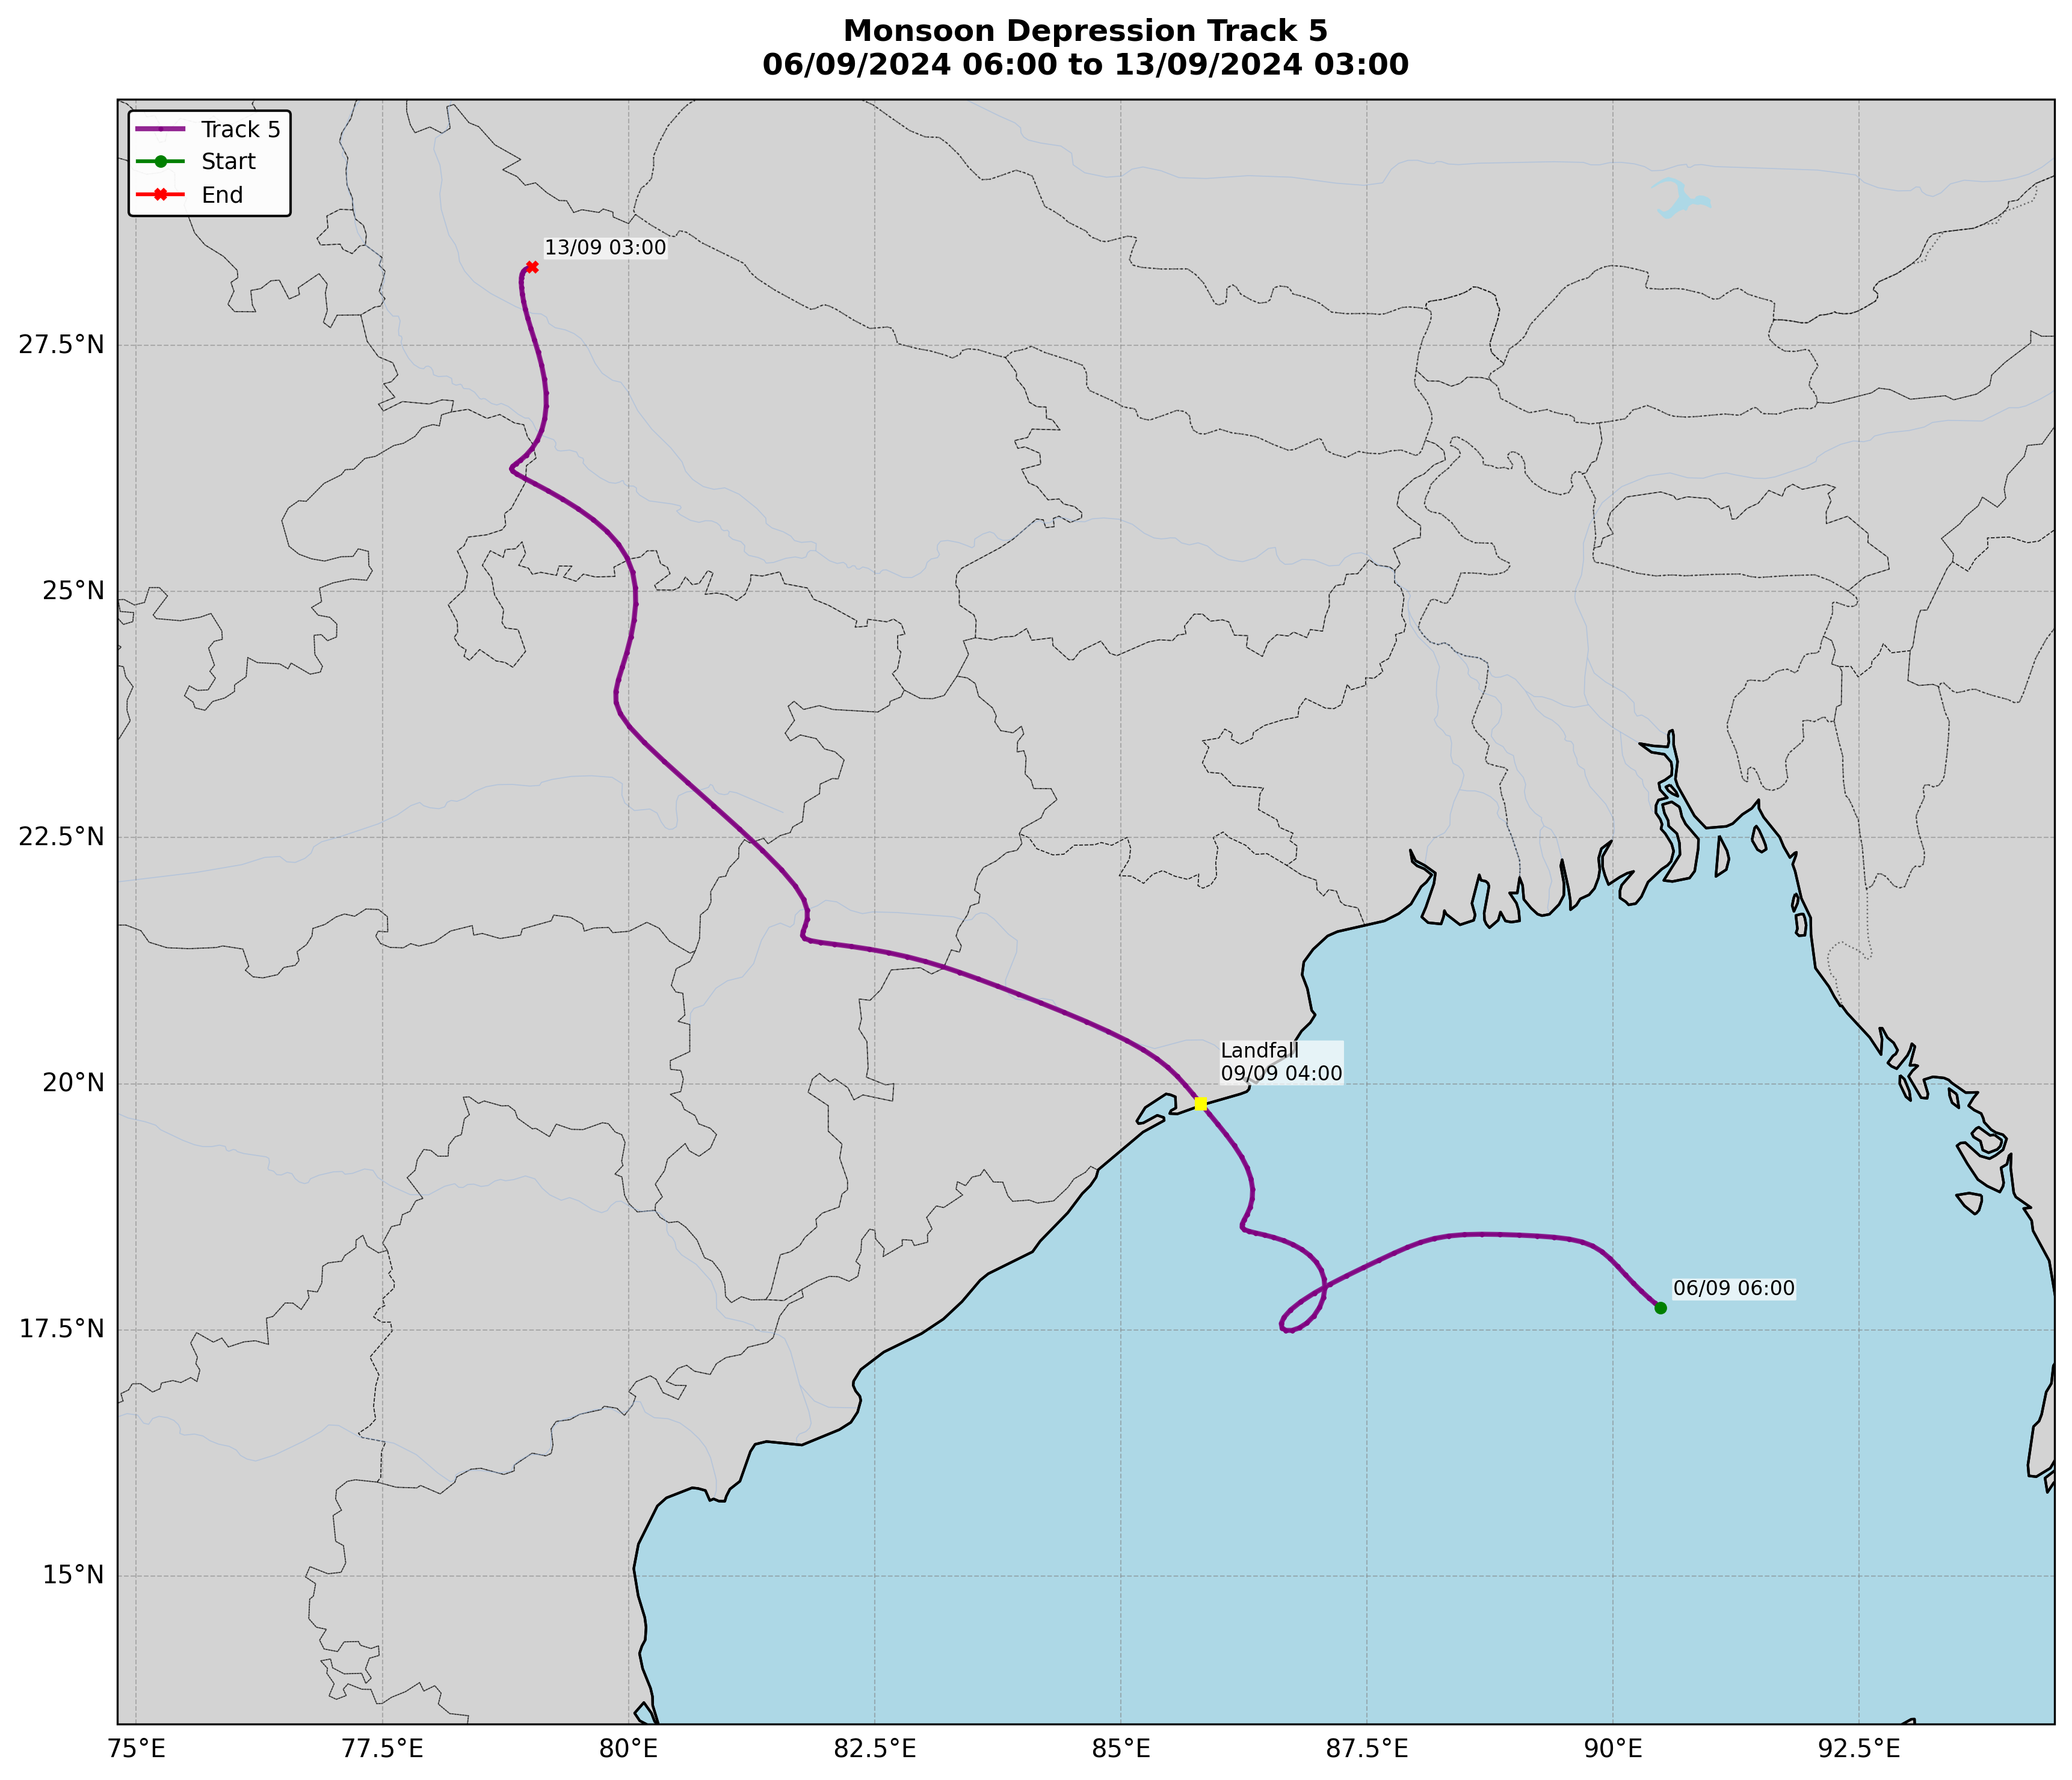
\includegraphics[width=0.95\textwidth]{../version5-with-no-ocean-masking/output/track_5/MD-track-5-detailed.png}

			\column{0.4\textwidth}
			\begin{block}{Statistics}
				\begin{itemize}
					\item Duration: 165 hours ($\sim$ 7 days)
					\item Category: long-lived MD
					\item Originated: over ocean
				\end{itemize}
			\end{block}
		\end{columns}
	\end{center}
\end{frame}

% 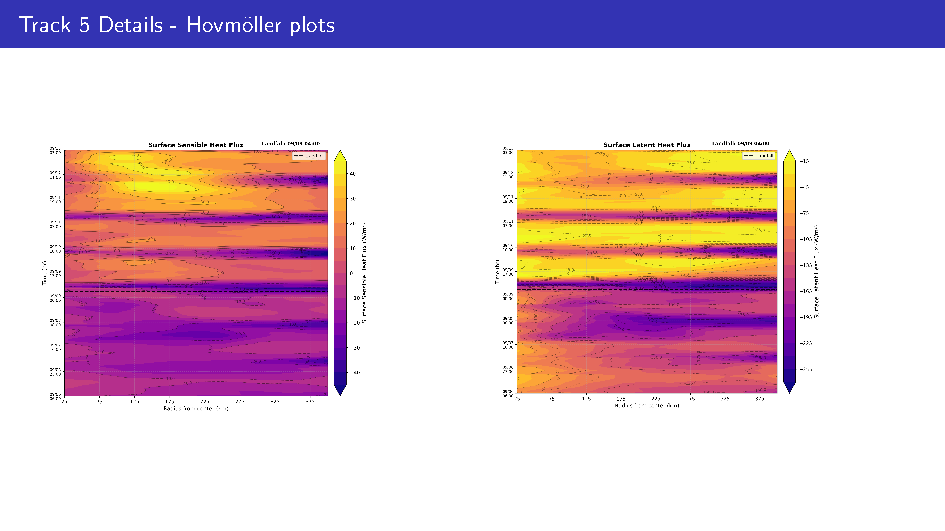
\includepdf[
% 	pages=-,
% 	scale=1,
% 	frame=true,
% 	pagecommand={\thispagestyle{empty}},  % Remove page numbers
% 	offset=0mm 0mm,       % Adjust position
% 	% templatesize={\textwidth}{\textheight} % Match template size
% ]{hovmoller-slides/hov-5.pdf}

% \begin{frame}{Track 5 Details - Precipitation and soil moisture over time along track}
% 	\begin{center}
% 		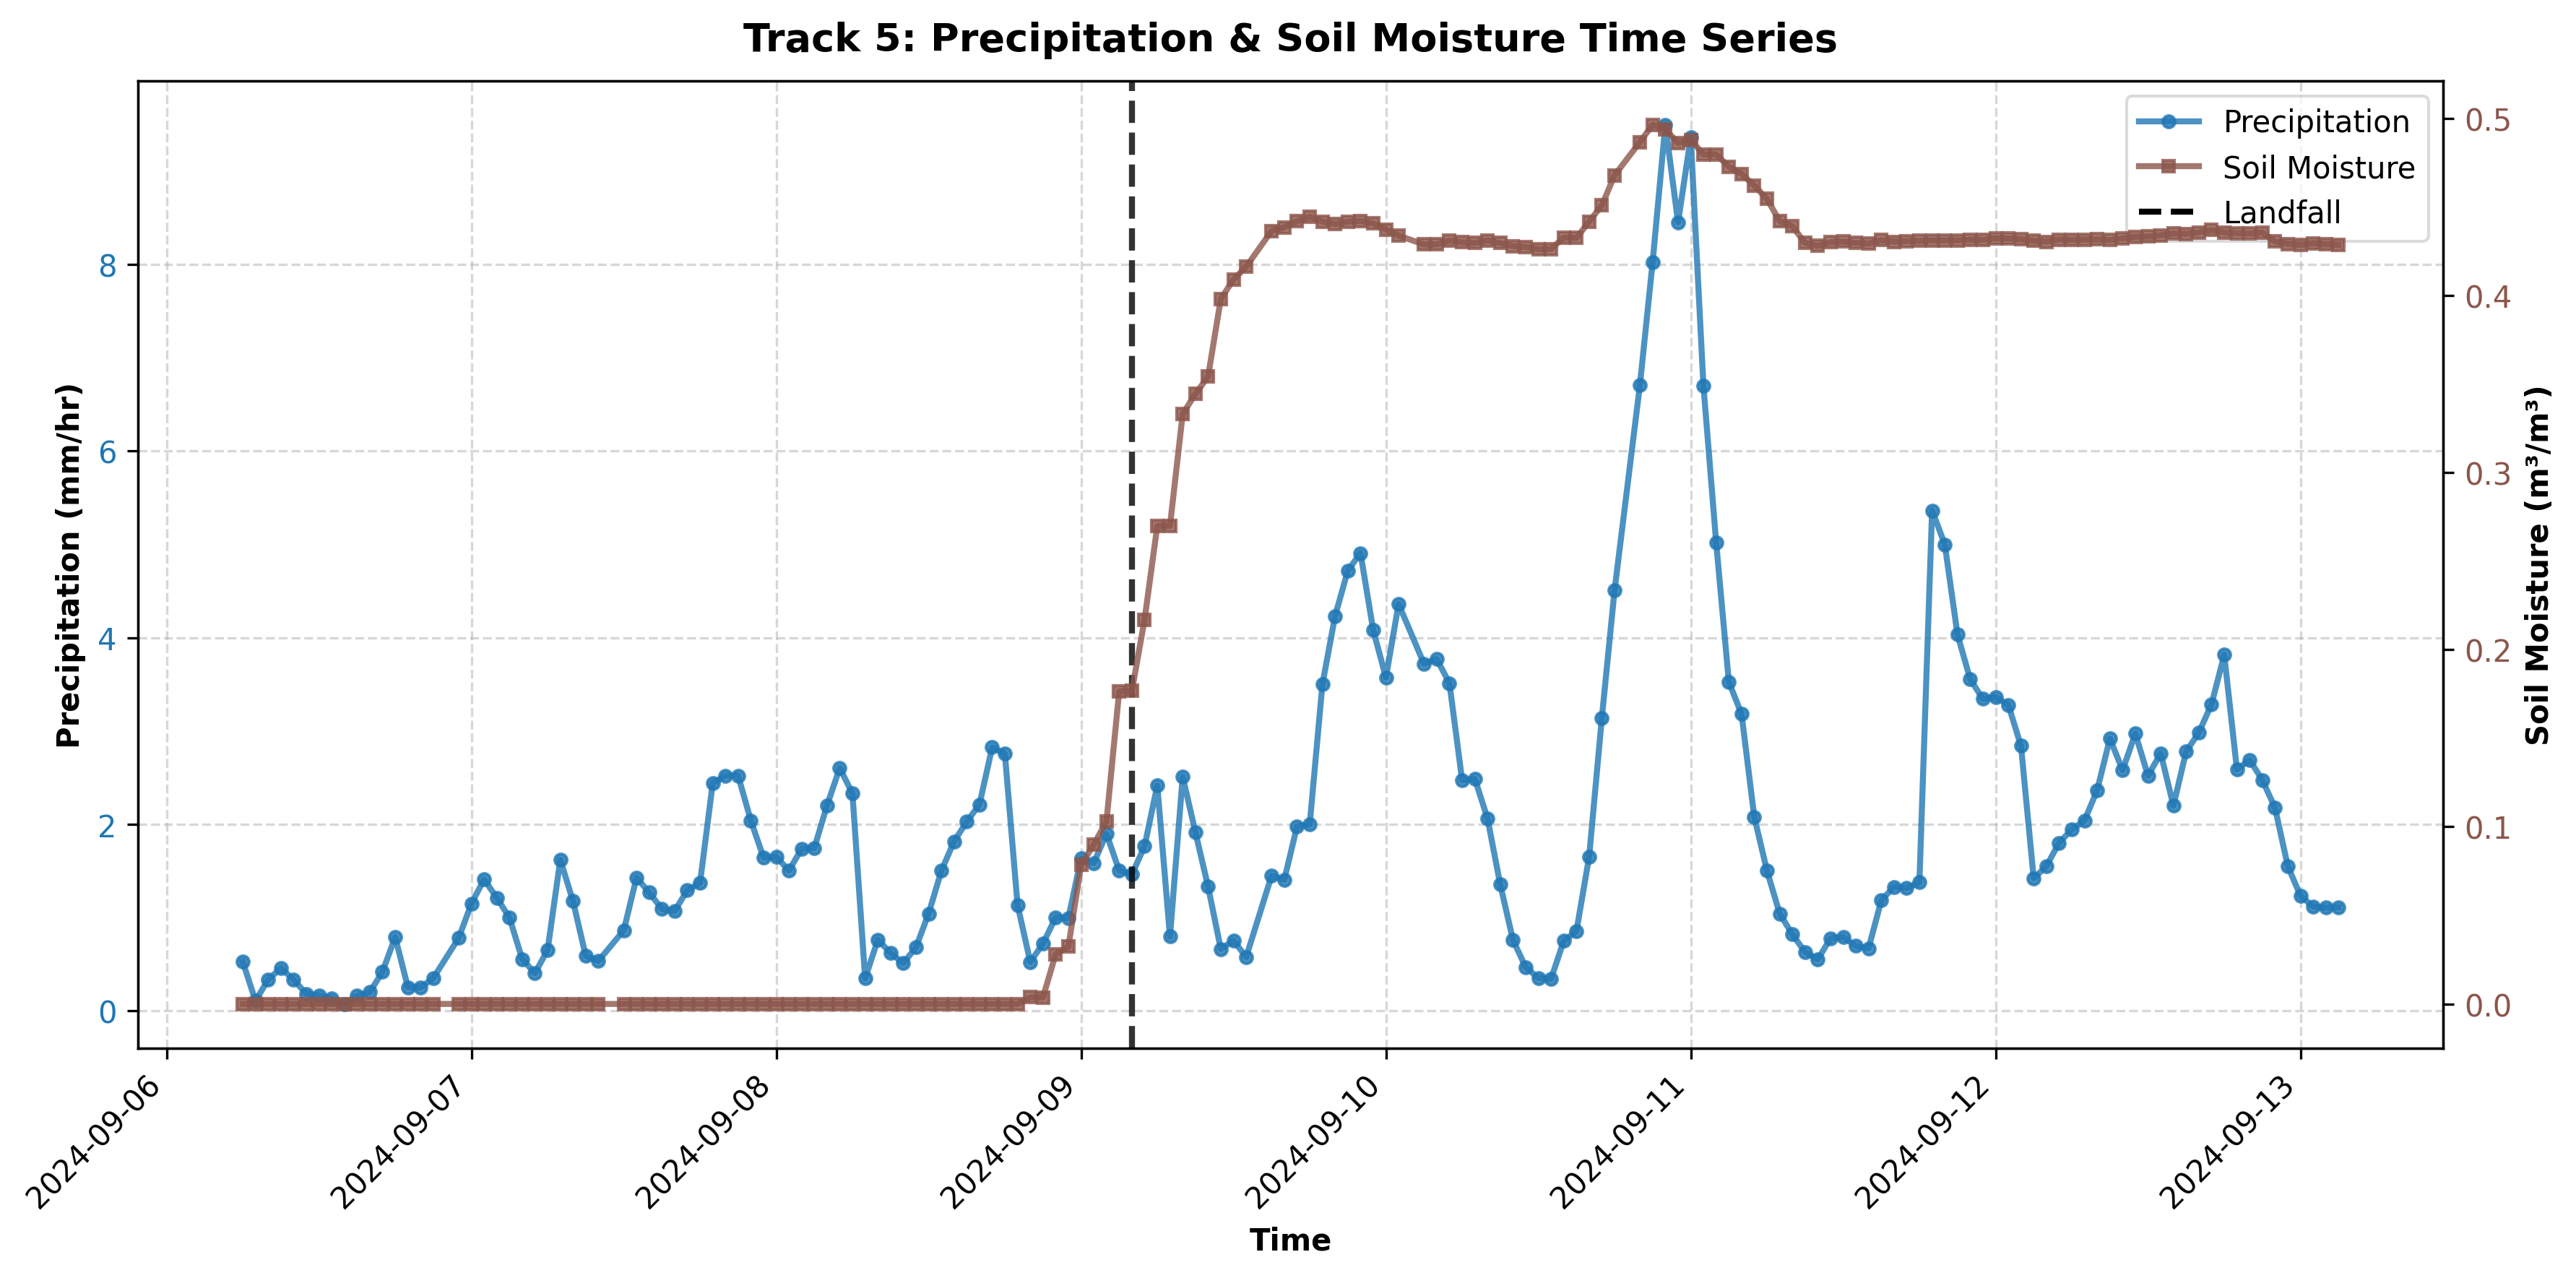
\includegraphics[width=0.8\textwidth]{../version1-with-no-ocean-masking/output/track_5/correlation_analysis/time_series/track_5_time_series.png}
% 	\end{center}
% \end{frame}

\begin{frame}{Track 5 Details - Translation speed of MD}
	\begin{center}
		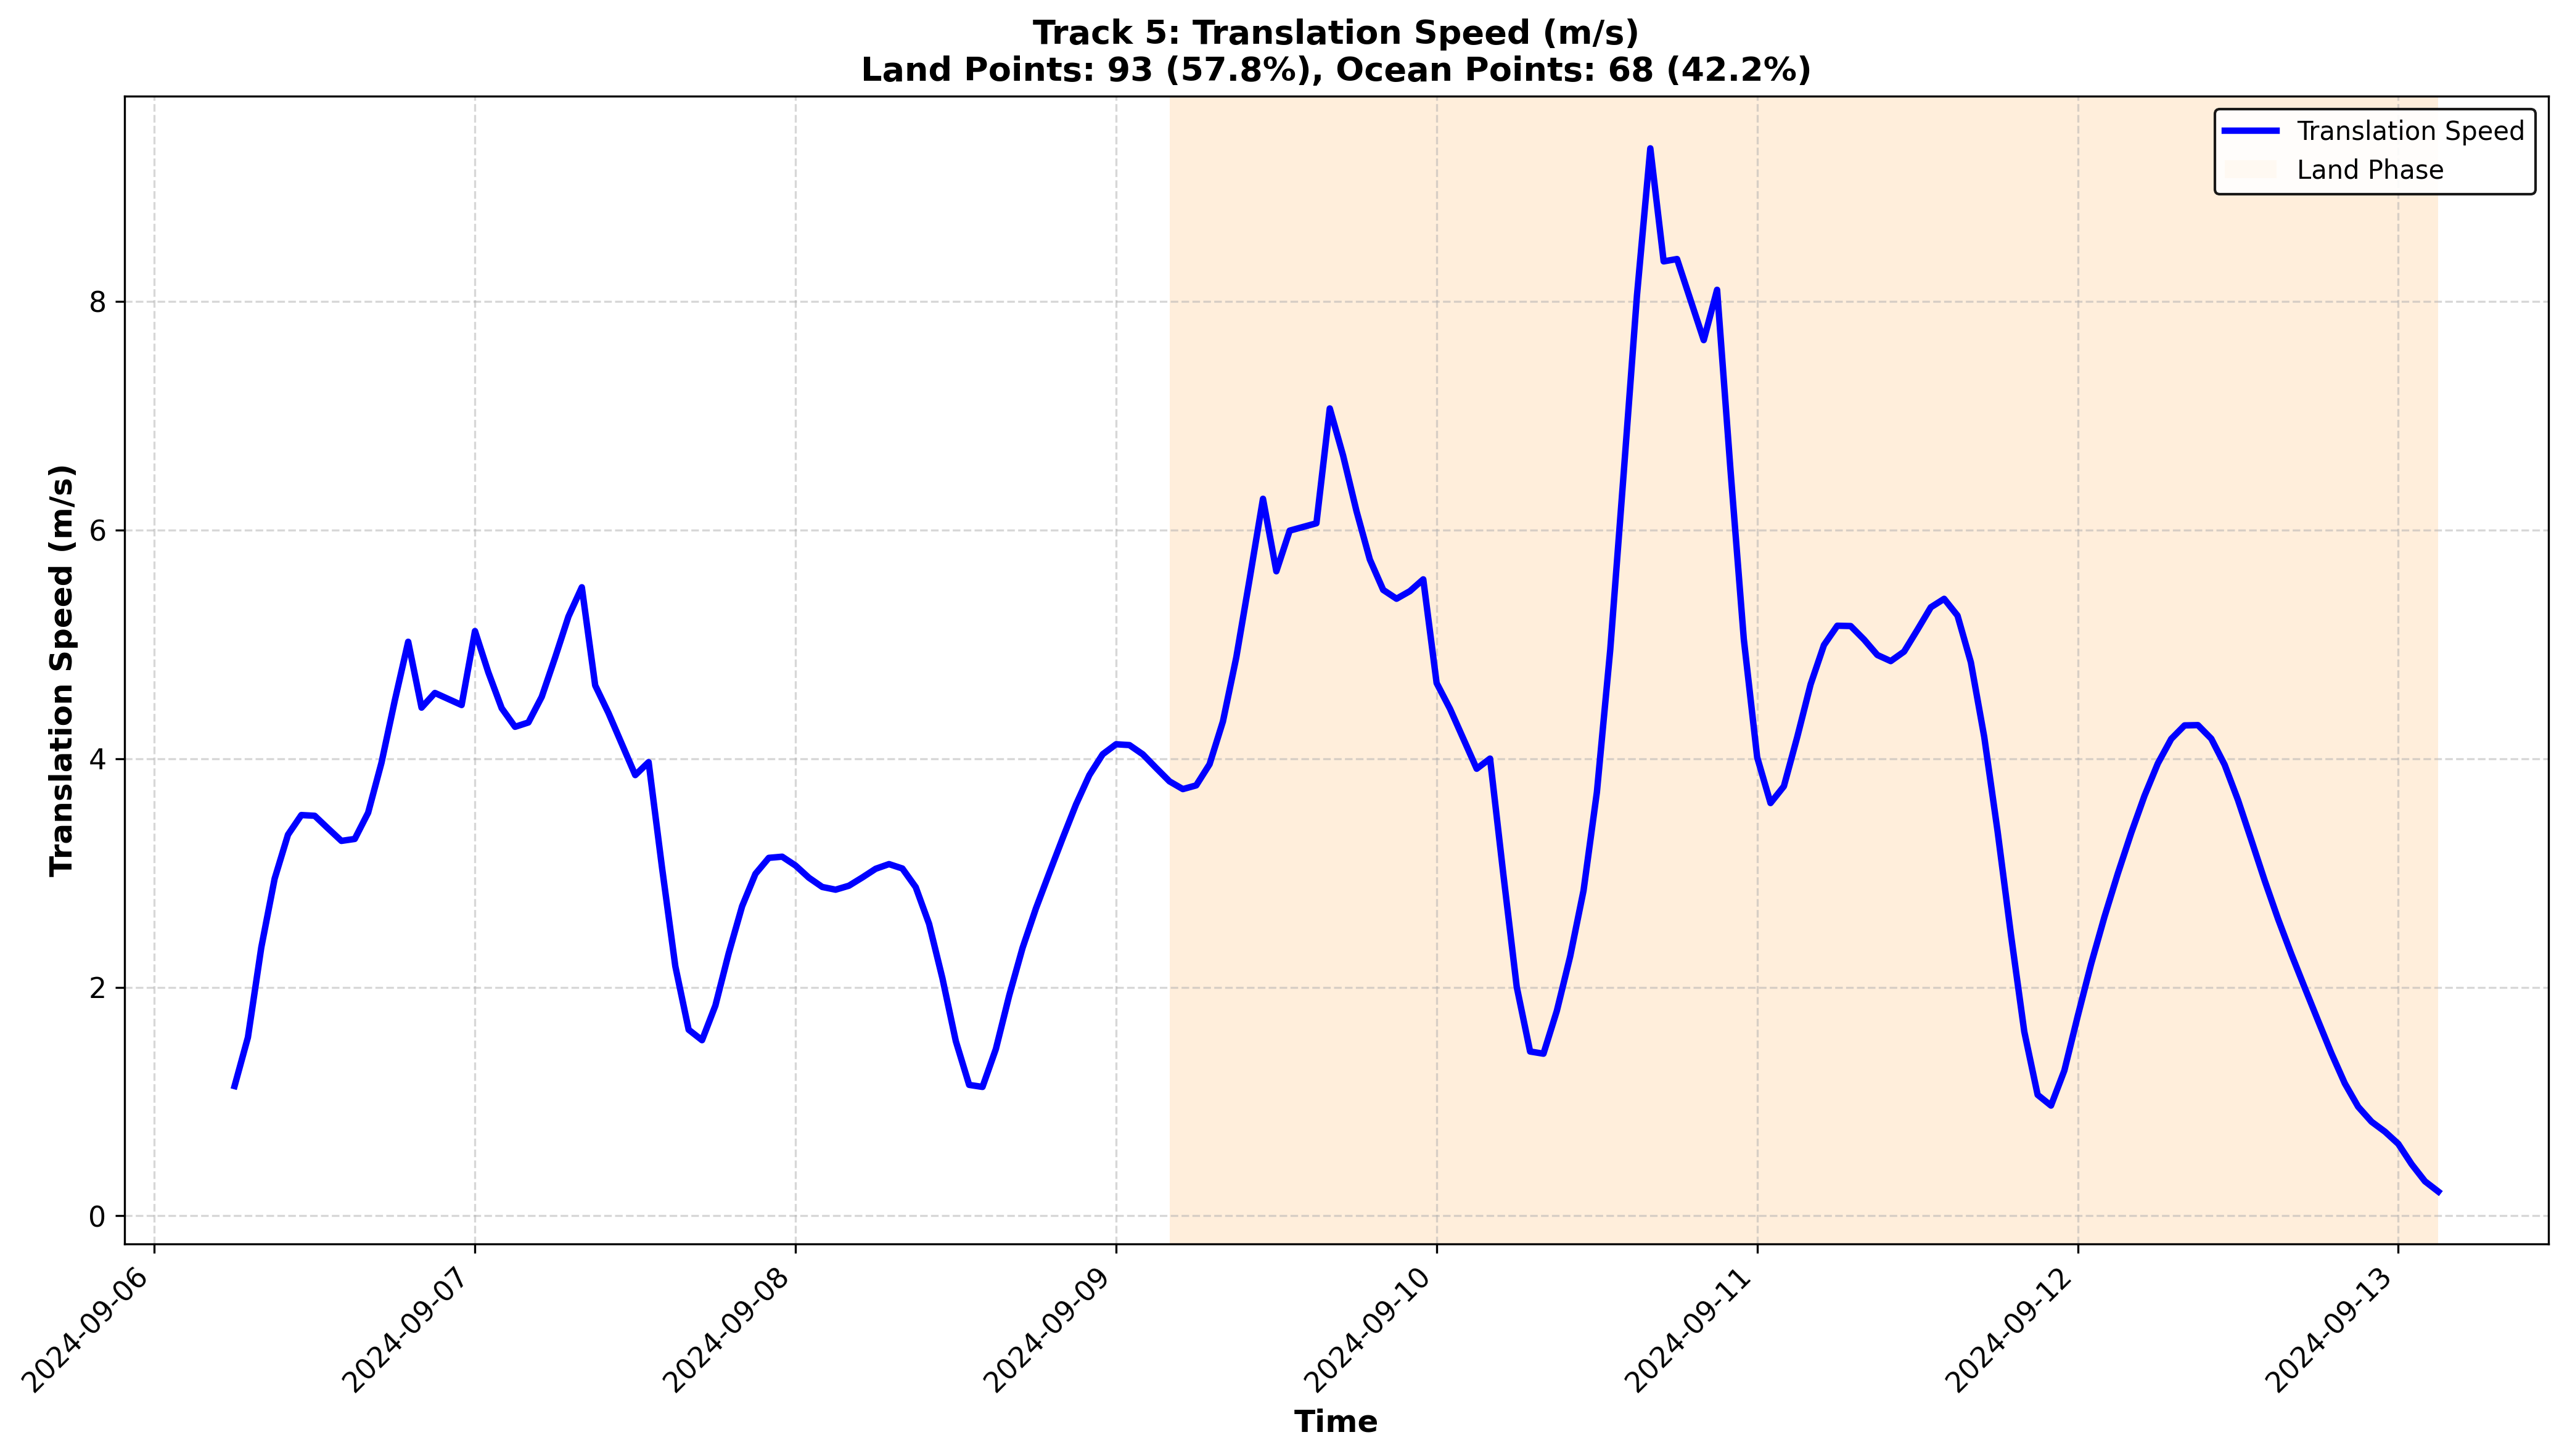
\includegraphics[width=0.8\textwidth]{../version5-with-no-ocean-masking/output/track_5/translational-speed/track_5_speed_ms.png}
	\end{center}
\end{frame}

\begin{frame}{Track 5 Details - Lag Correlation}
	\begin{center}
		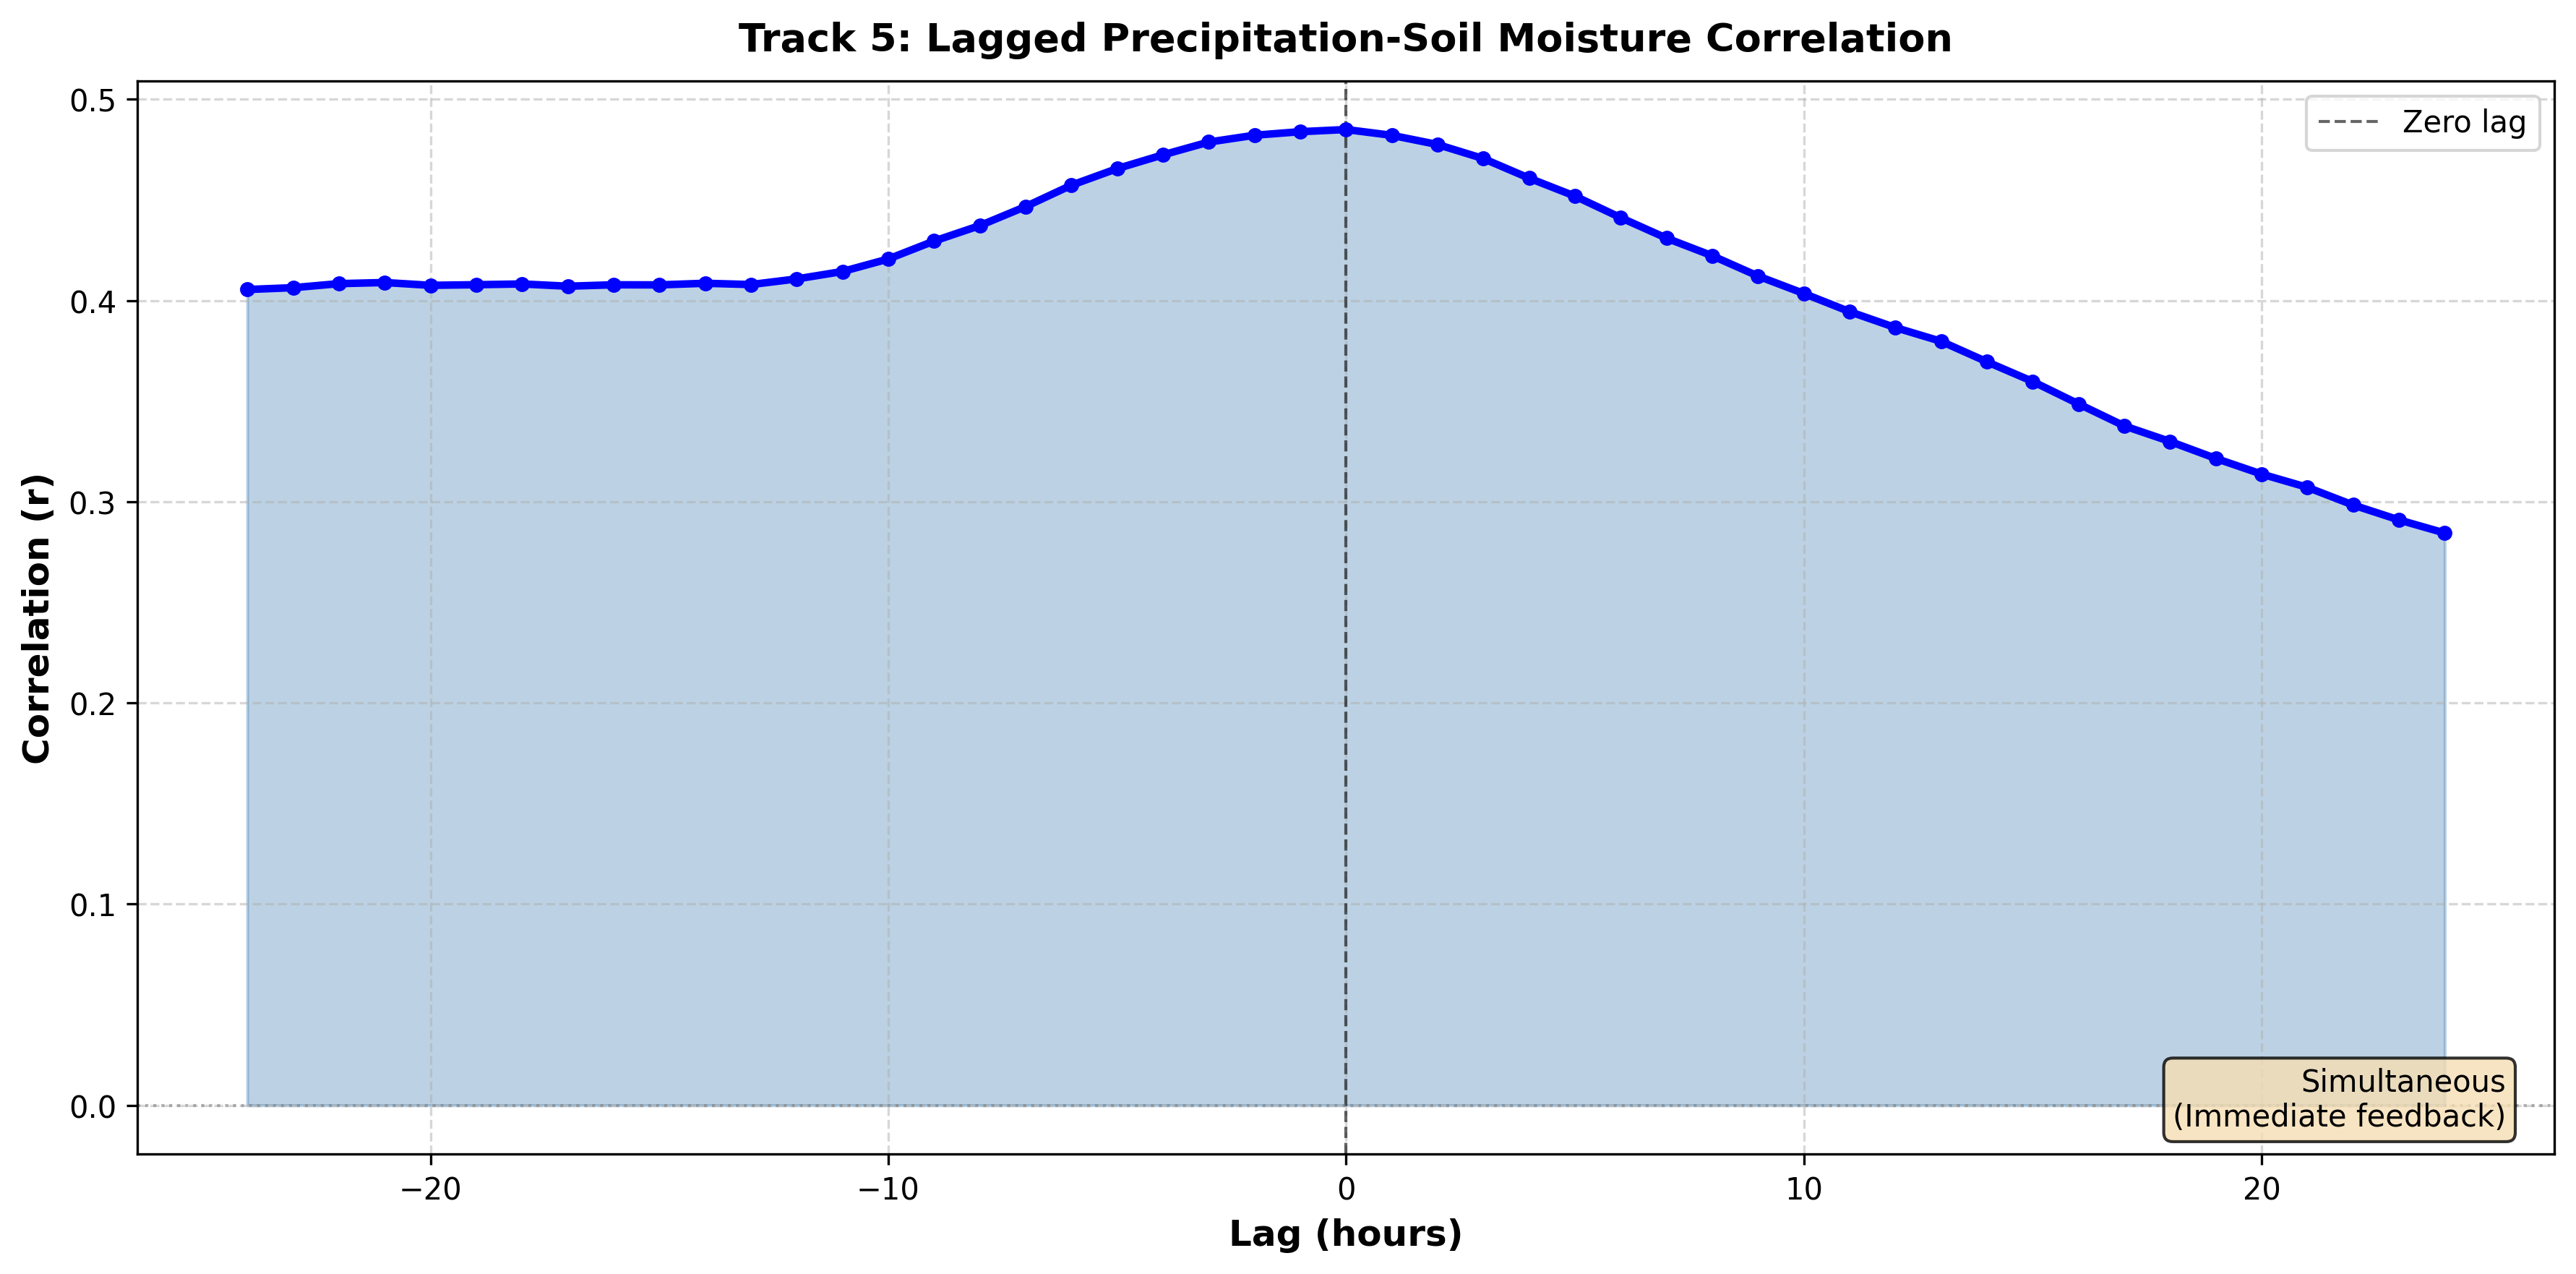
\includegraphics[width=0.8\textwidth]{../version5-with-no-ocean-masking/output/track_5/correlation_analysis/lag_correlation/track_5_lag_corr.png}
	\end{center}
\end{frame}

\begin{frame}{Track 5 Details - TP - SWVL1 Correlation}
	\begin{center}
		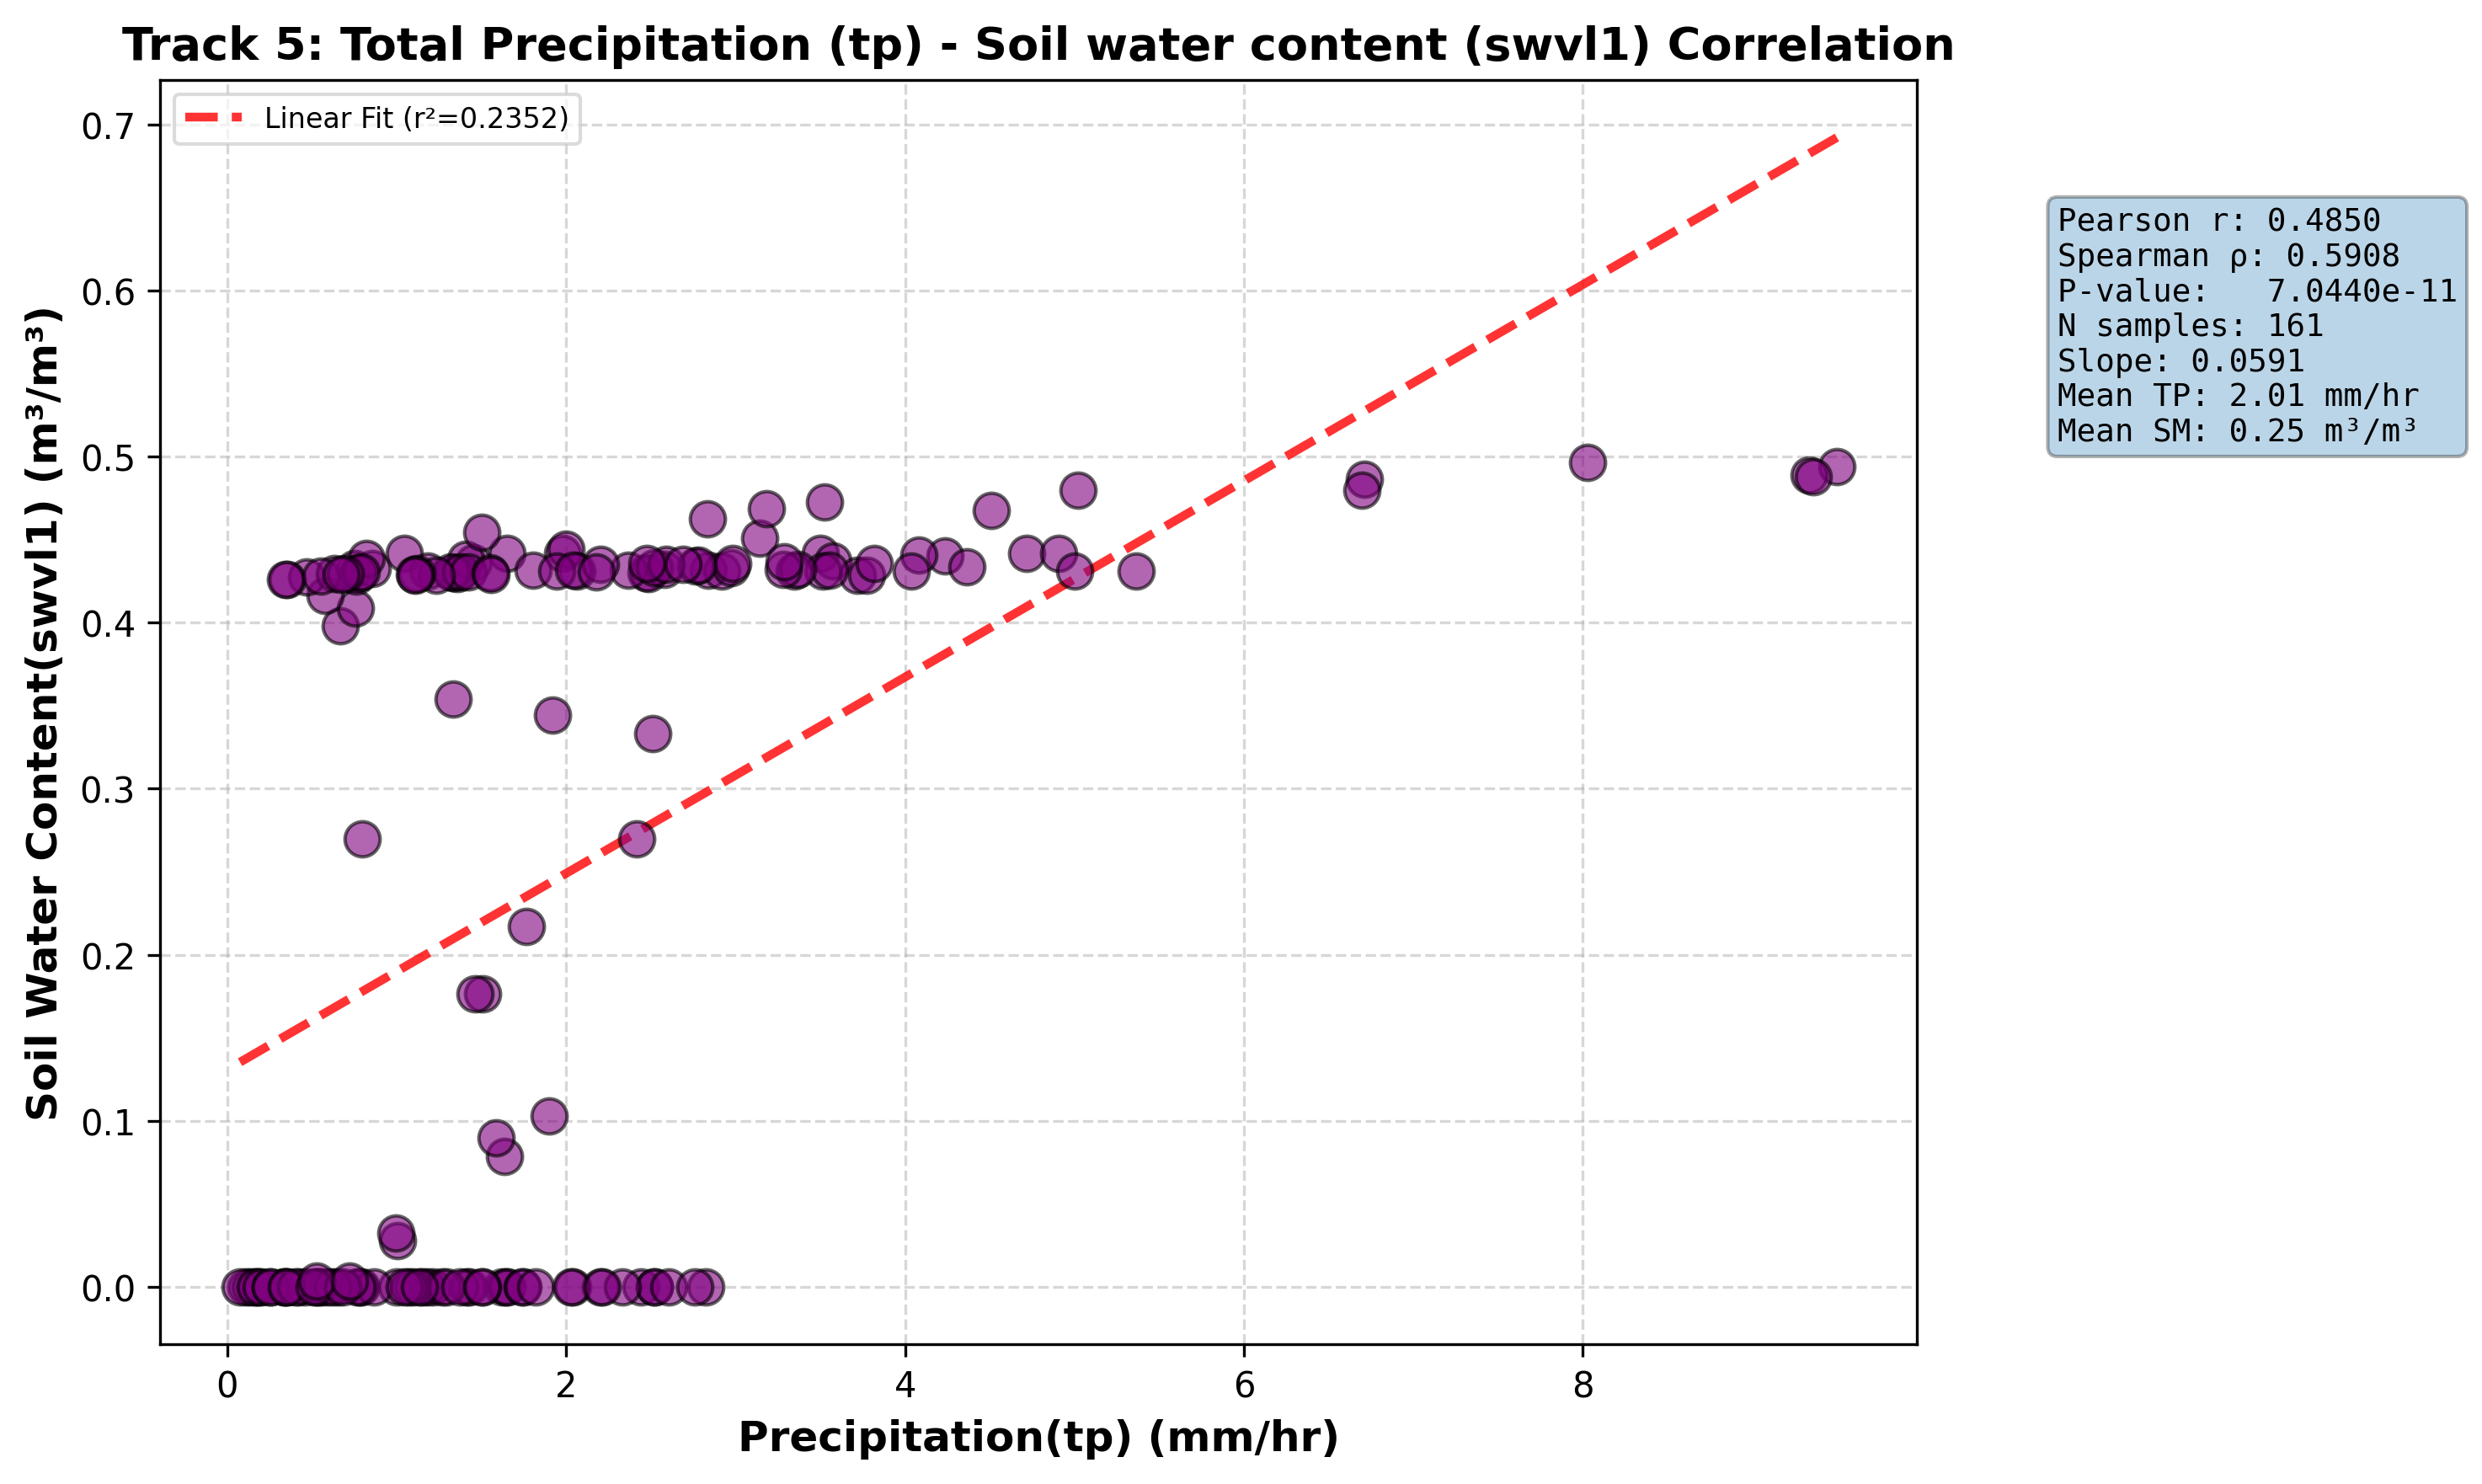
\includegraphics[width=0.7\textwidth]{../version5-with-no-ocean-masking/output/track_5/correlation_analysis/scatter_plots/track_5_scatter.png}
	\end{center}
\end{frame}

\begin{frame}{Track 5 Details - Spatial distribution of TP and SWVL1}
	\begin{center}
		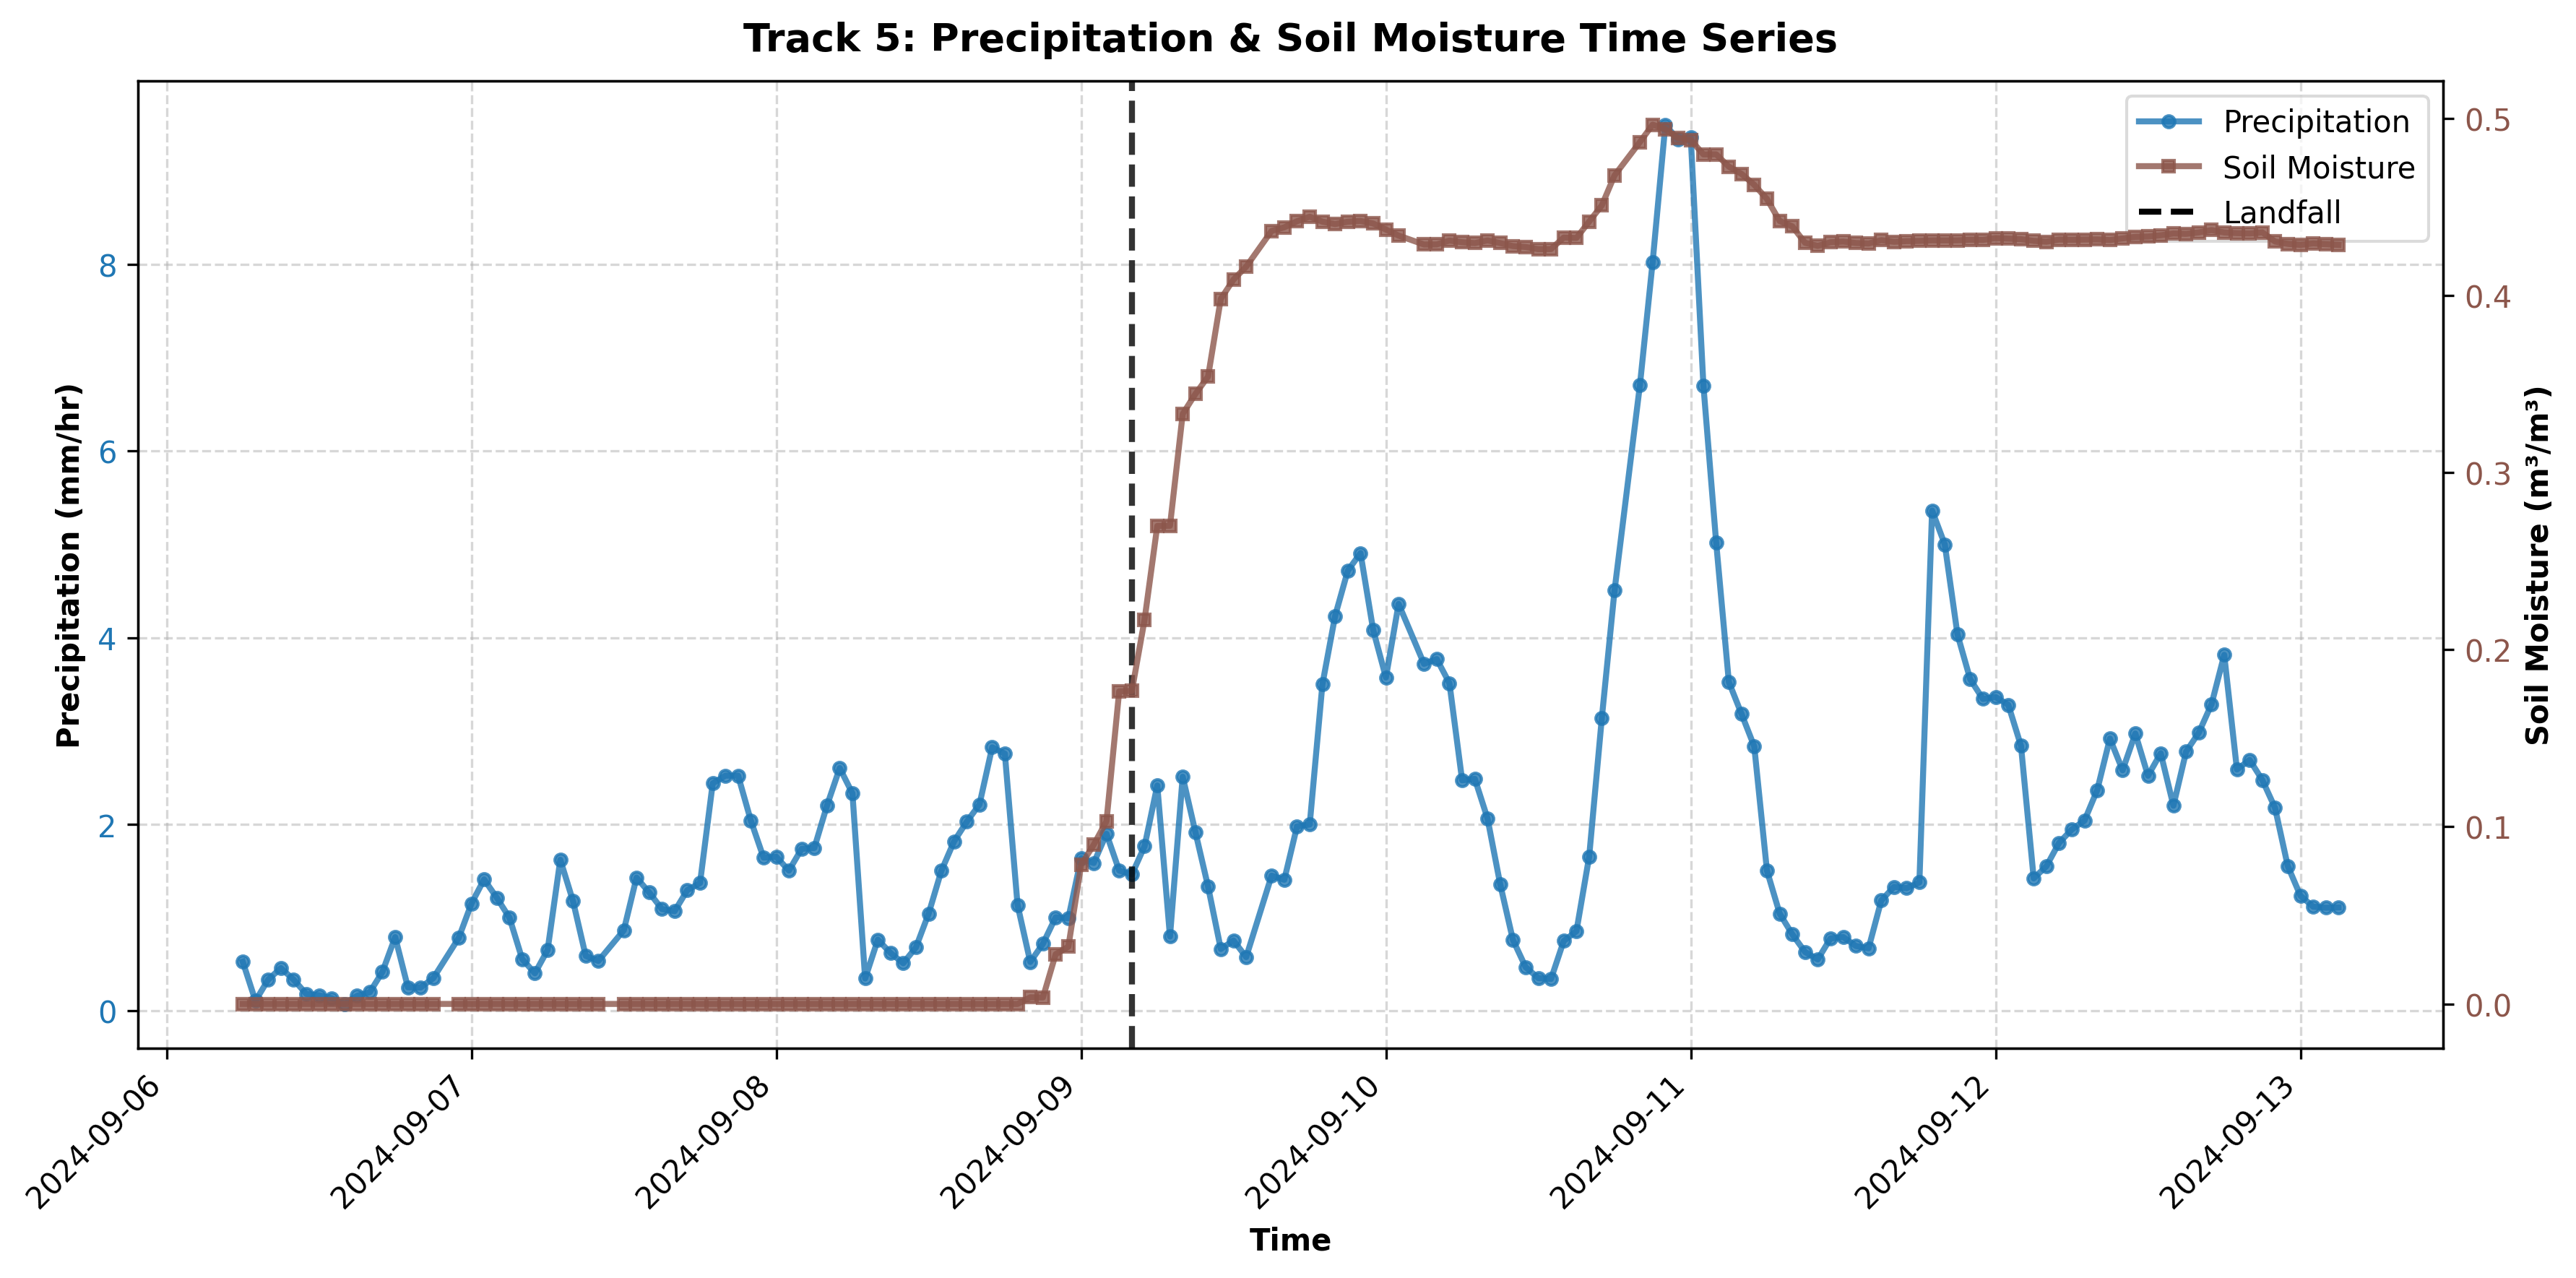
\includegraphics[width=0.7\textwidth]{../version5-with-no-ocean-masking/output/track_5/correlation_analysis/time_series/track_5_tp_sm_time_series.png}
	\end{center}
\end{frame}

% \begin{frame}{Track 5 Details - Heat fluxes transition}
% 	\begin{center}
% 		\includegraphics[width=0.8\textwidth]{../version5-with-no-ocean-masking/output/track_5/flux_analysis/track_5_analysis/track_5_heat_fluxes_trasnsition.png}
% 	\end{center}
% \end{frame}

\begin{frame}{Track 5 Details - Heat flux analysis}
	\begin{center}
		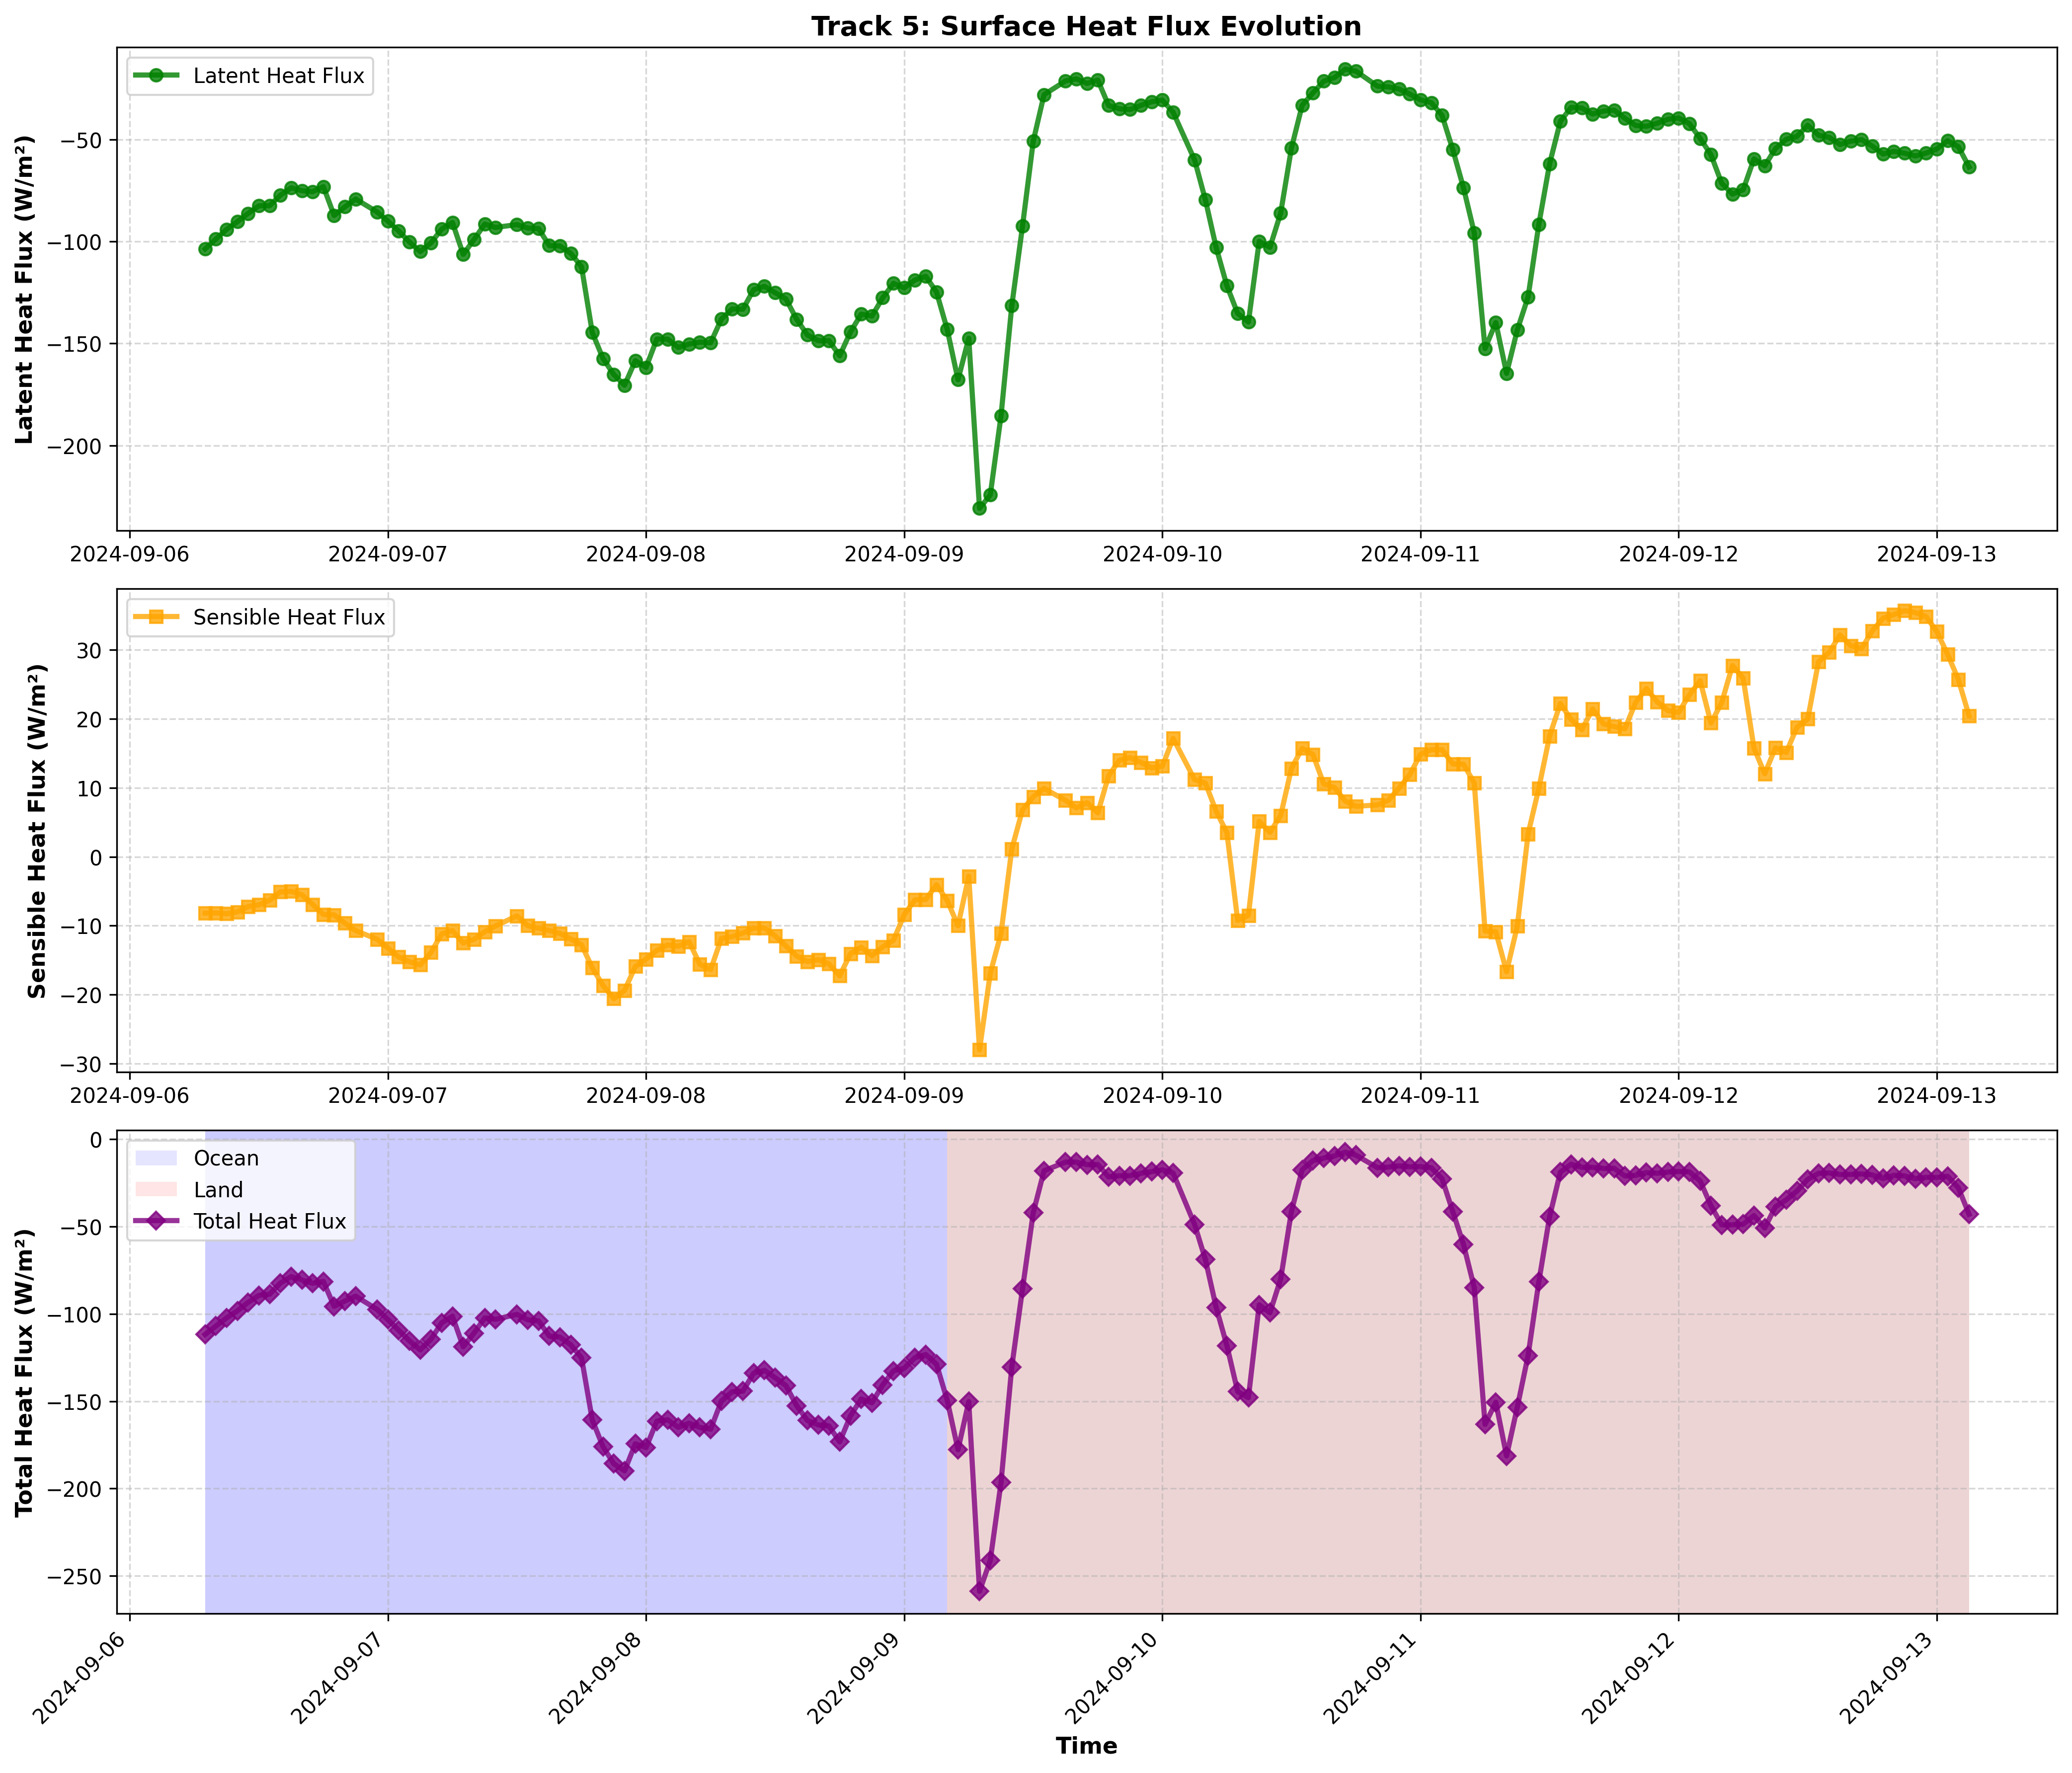
\includegraphics[width=0.6\textwidth]{../version5-with-no-ocean-masking/output/track_5/heat_flux_analysis/track_5_heat_flux_timeseries.png}
	\end{center}
\end{frame}

% %%%%%%%%%%%%%%%% Track 6 %%%%%%%%%%%%%%
\begin{frame}{Track 6 Details}
	\begin{center}
		\begin{columns}[T]
			\column{0.6\textwidth}
			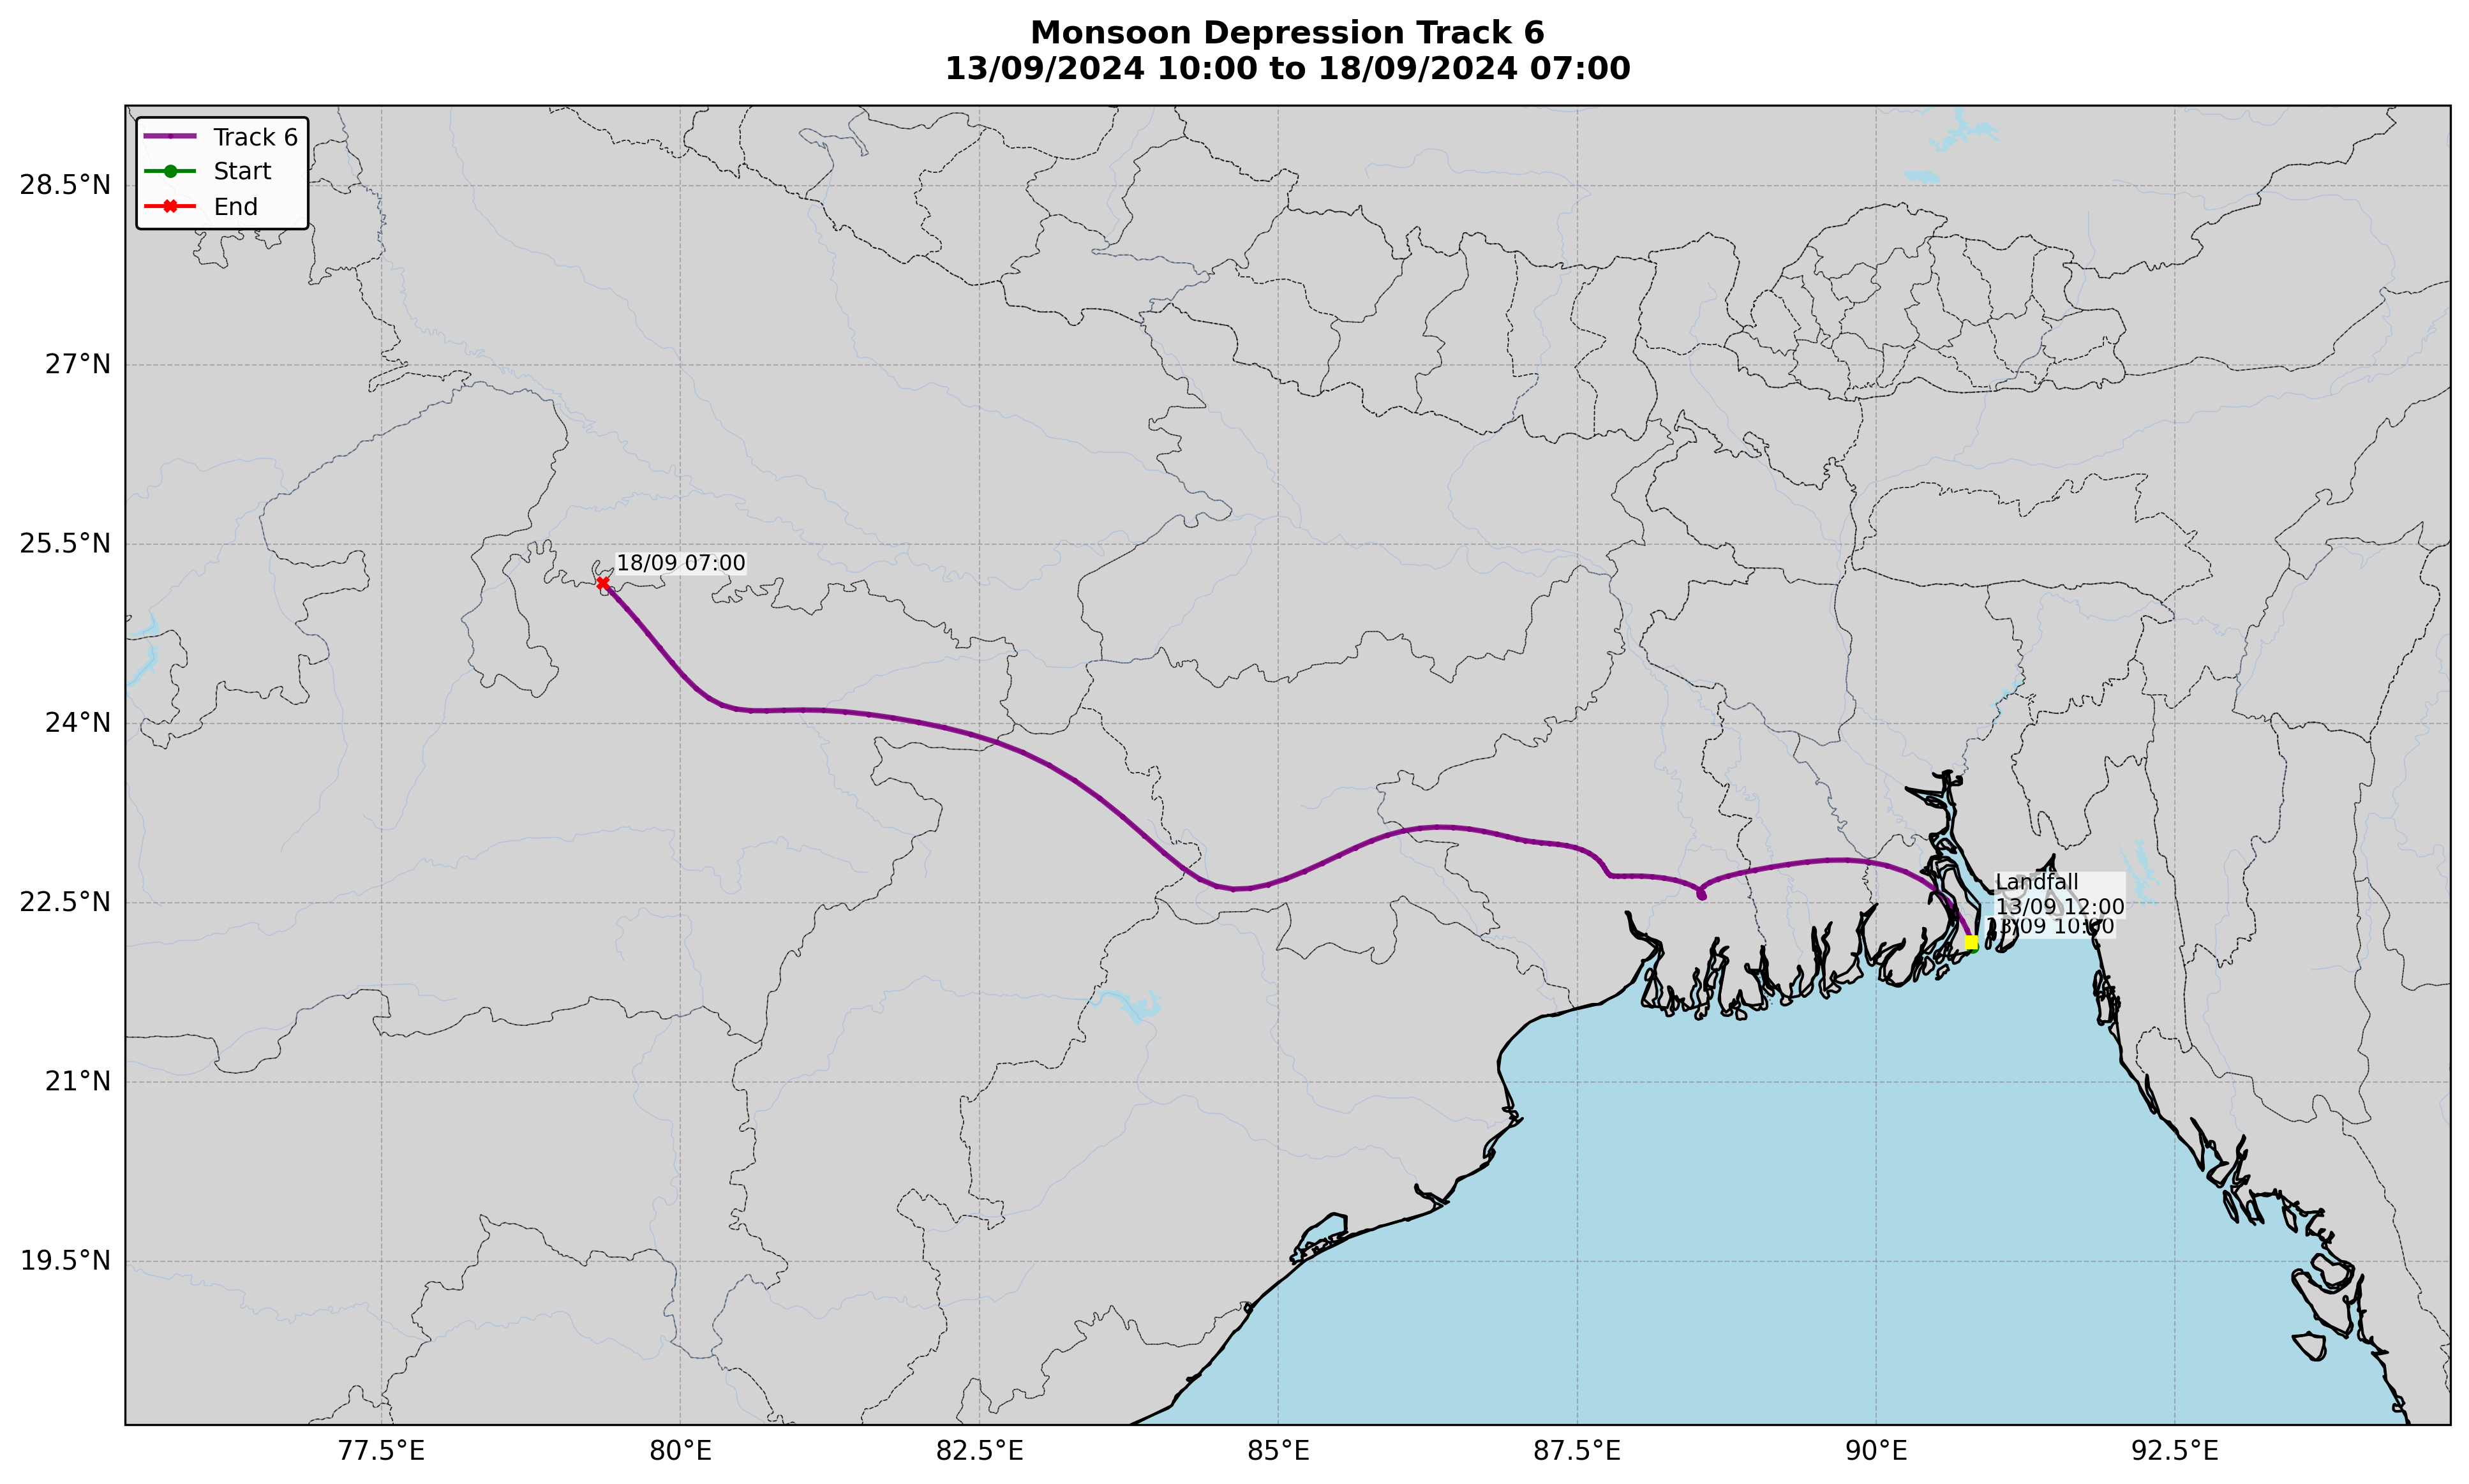
\includegraphics[width=0.95\textwidth]{../version5-with-no-ocean-masking/output/track_6/MD-track-6-detailed.png}

			\column{0.4\textwidth}
			\begin{block}{Statistics}
				\begin{itemize}
					\item Duration: 117 hours ($\sim$ 5 days)
					\item Category: long-lived MD
					\item Originated: over land
				\end{itemize}
			\end{block}
		\end{columns}
	\end{center}
\end{frame}

% 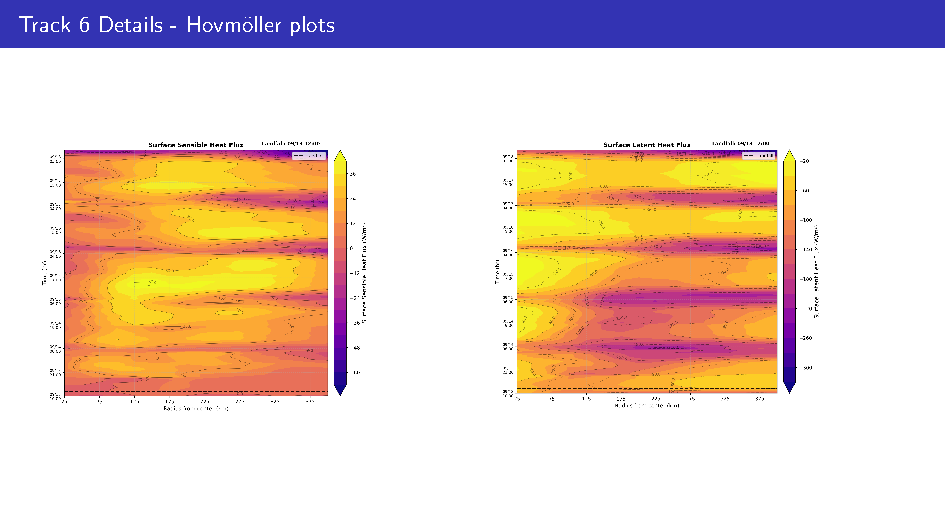
\includepdf[
% 	pages=-,
% 	scale=1,
% 	frame=true,
% 	pagecommand={\thispagestyle{empty}},  % Remove page numbers
% 	offset=0mm 0mm,       % Adjust position
% 	% templatesize={\textwidth}{\textheight} % Match template size
% ]{hovmoller-slides/hov-6.pdf}

% \begin{frame}{Track 6 Details - Precipitation and soil moisture over time along track}
% 	\begin{center}
% 		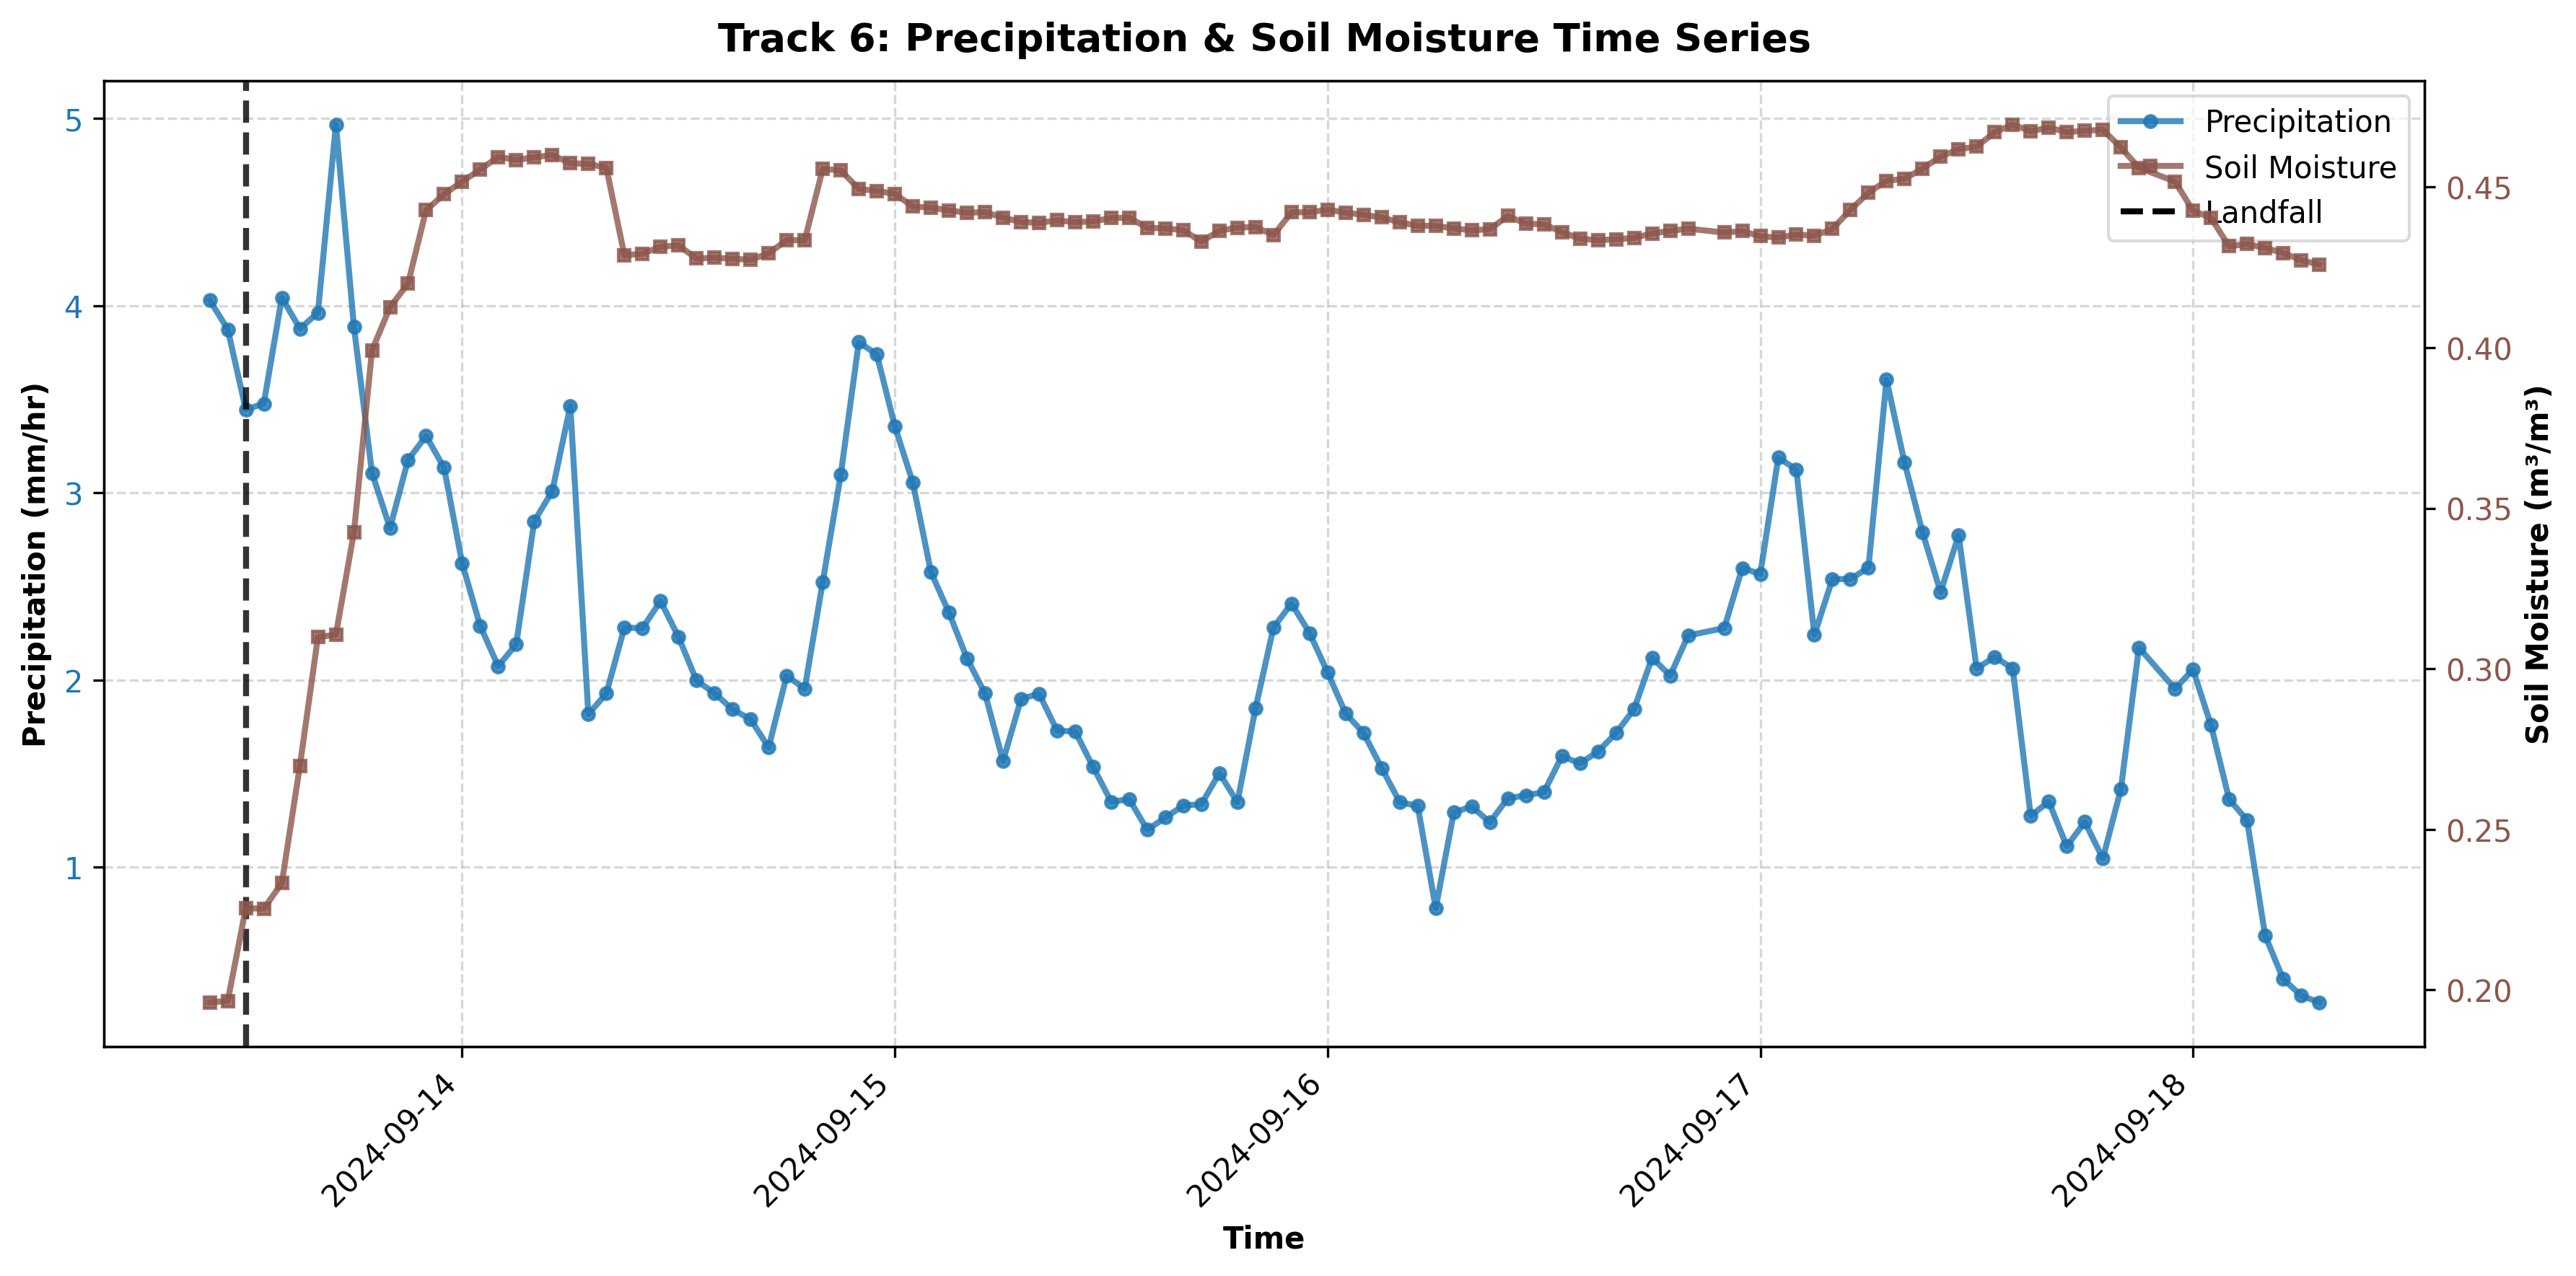
\includegraphics[width=0.8\textwidth]{../version1-with-no-ocean-masking/output/track_6/correlation_analysis/time_series/track_6_time_series.png}
% 	\end{center}
% \end{frame}

\begin{frame}{Track 6 Details - Translation speed of MD}
	\begin{center}
		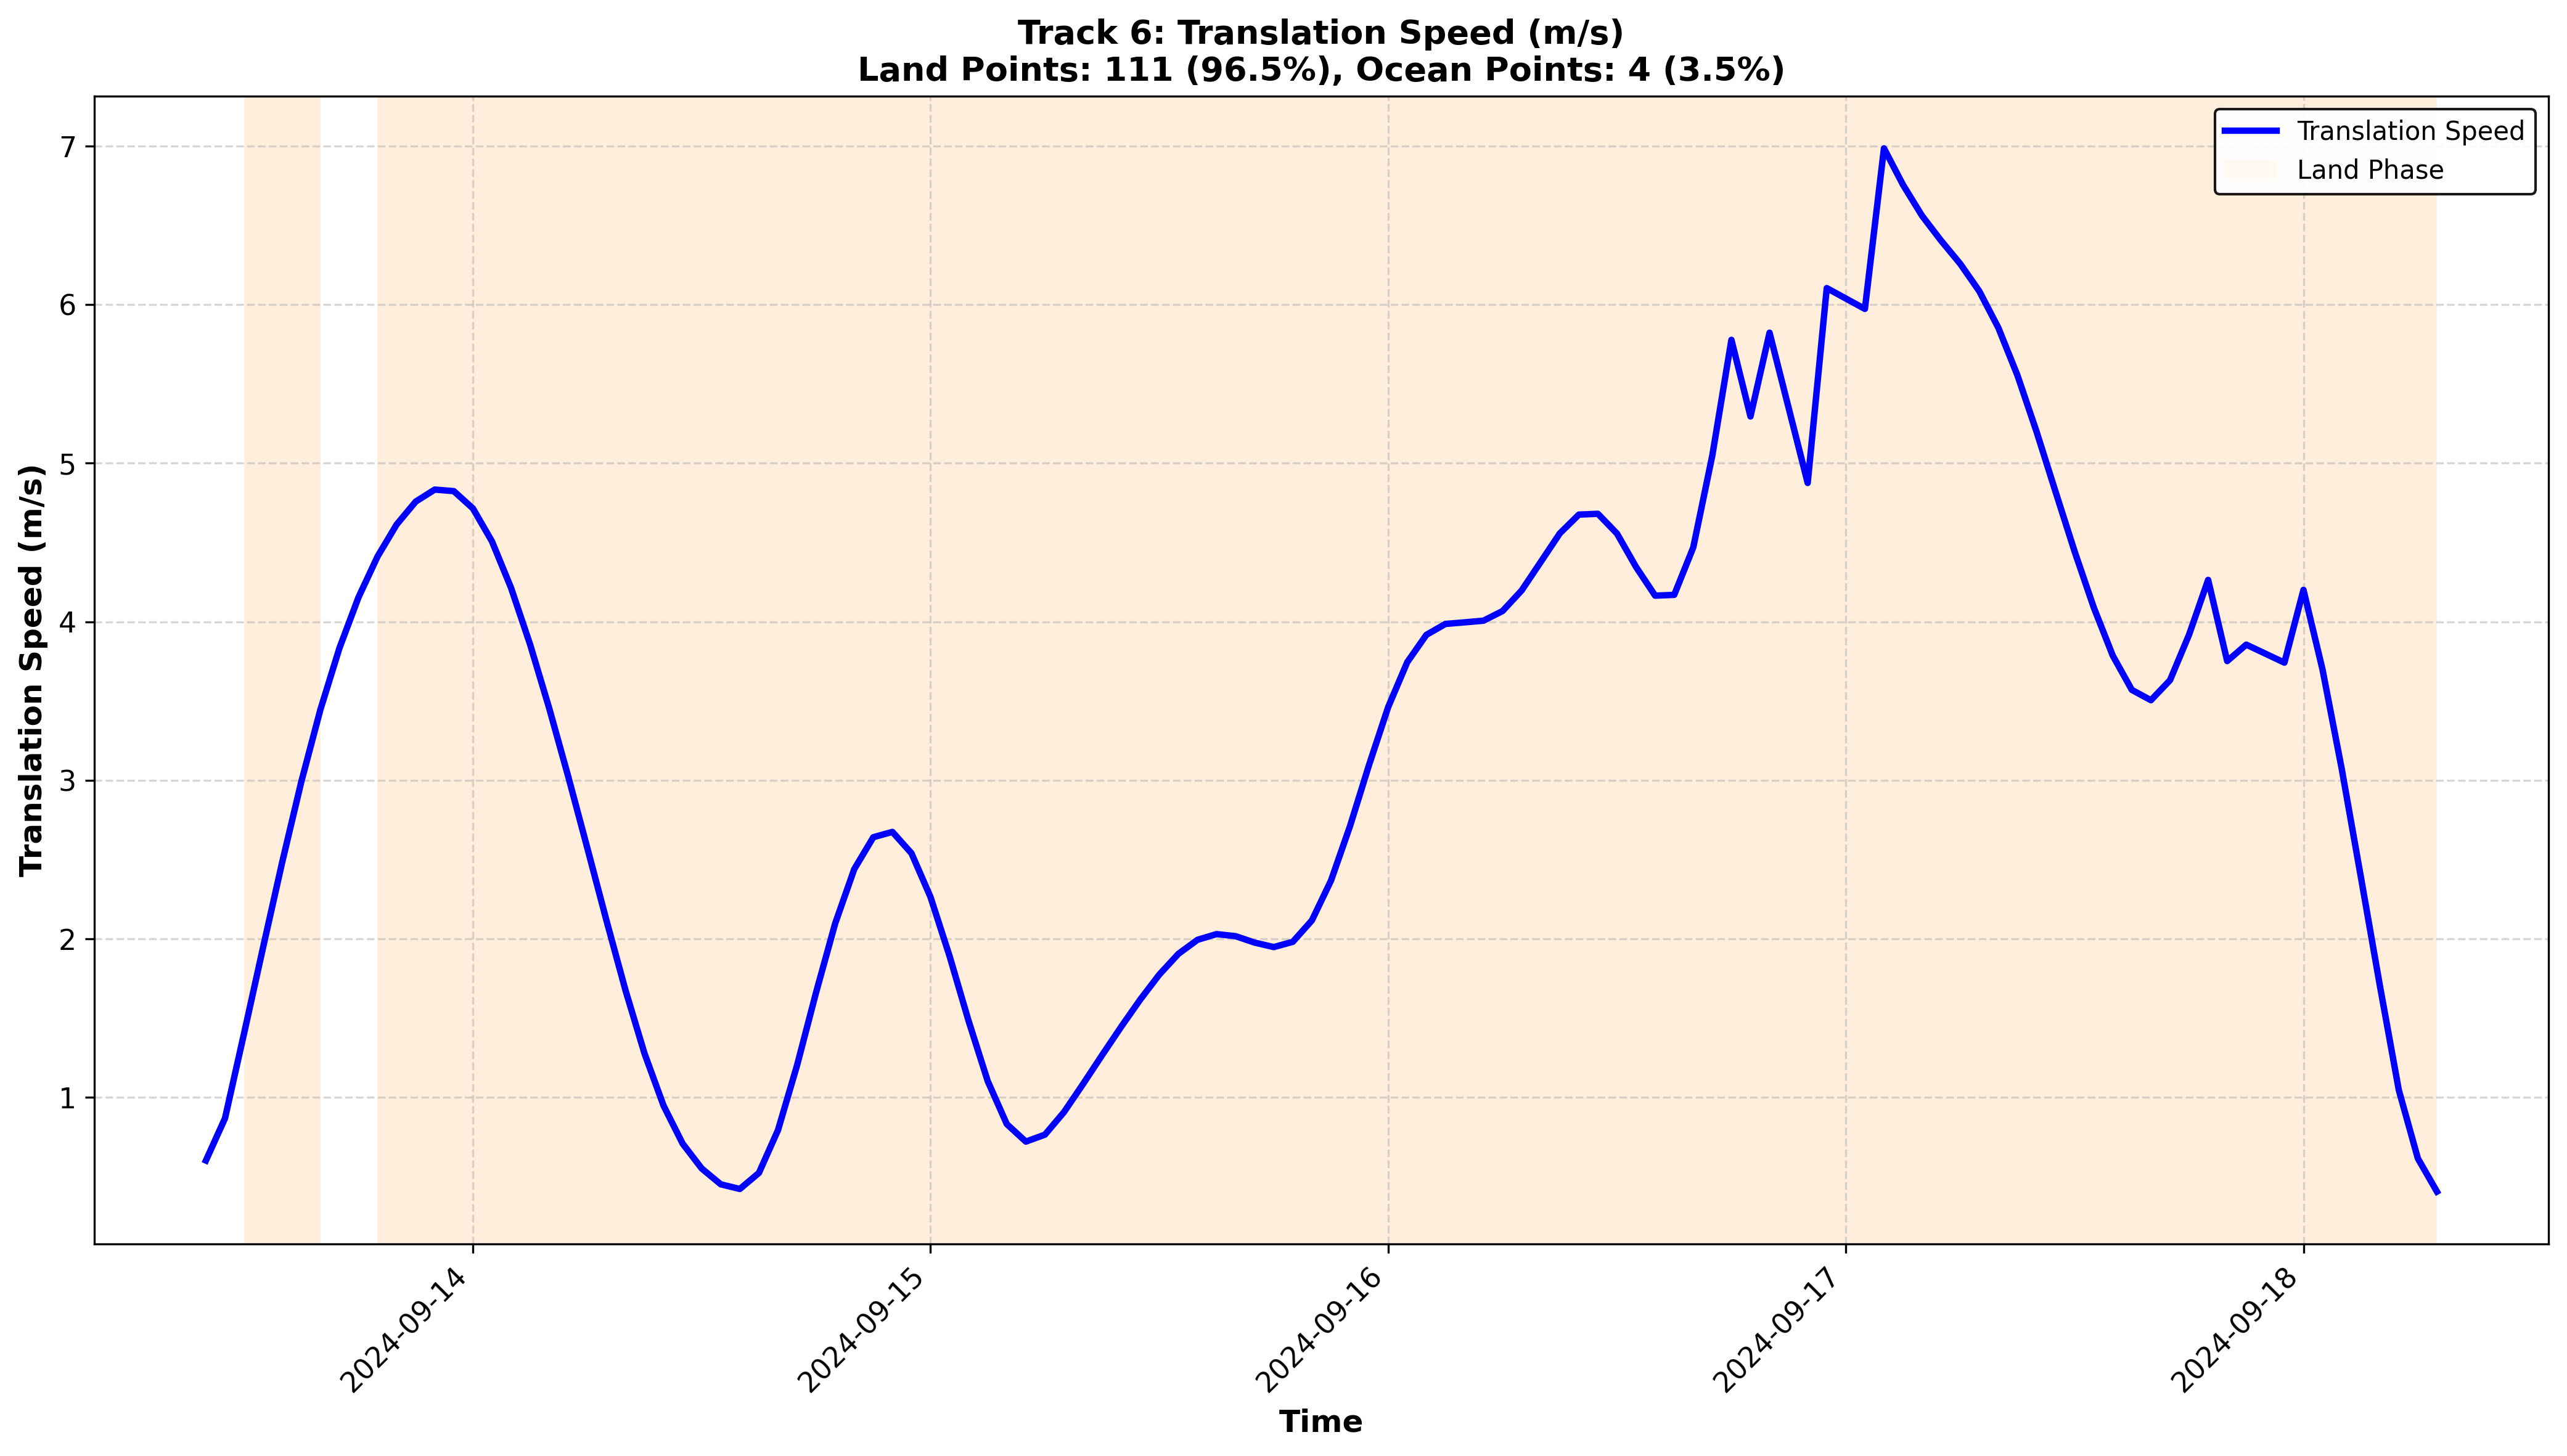
\includegraphics[width=0.8\textwidth]{../version5-with-no-ocean-masking/output/track_6/translational-speed/track_6_speed_ms.png}
	\end{center}
\end{frame}

\begin{frame}{Track 6 Details - Lag Correlation}
	\begin{center}
		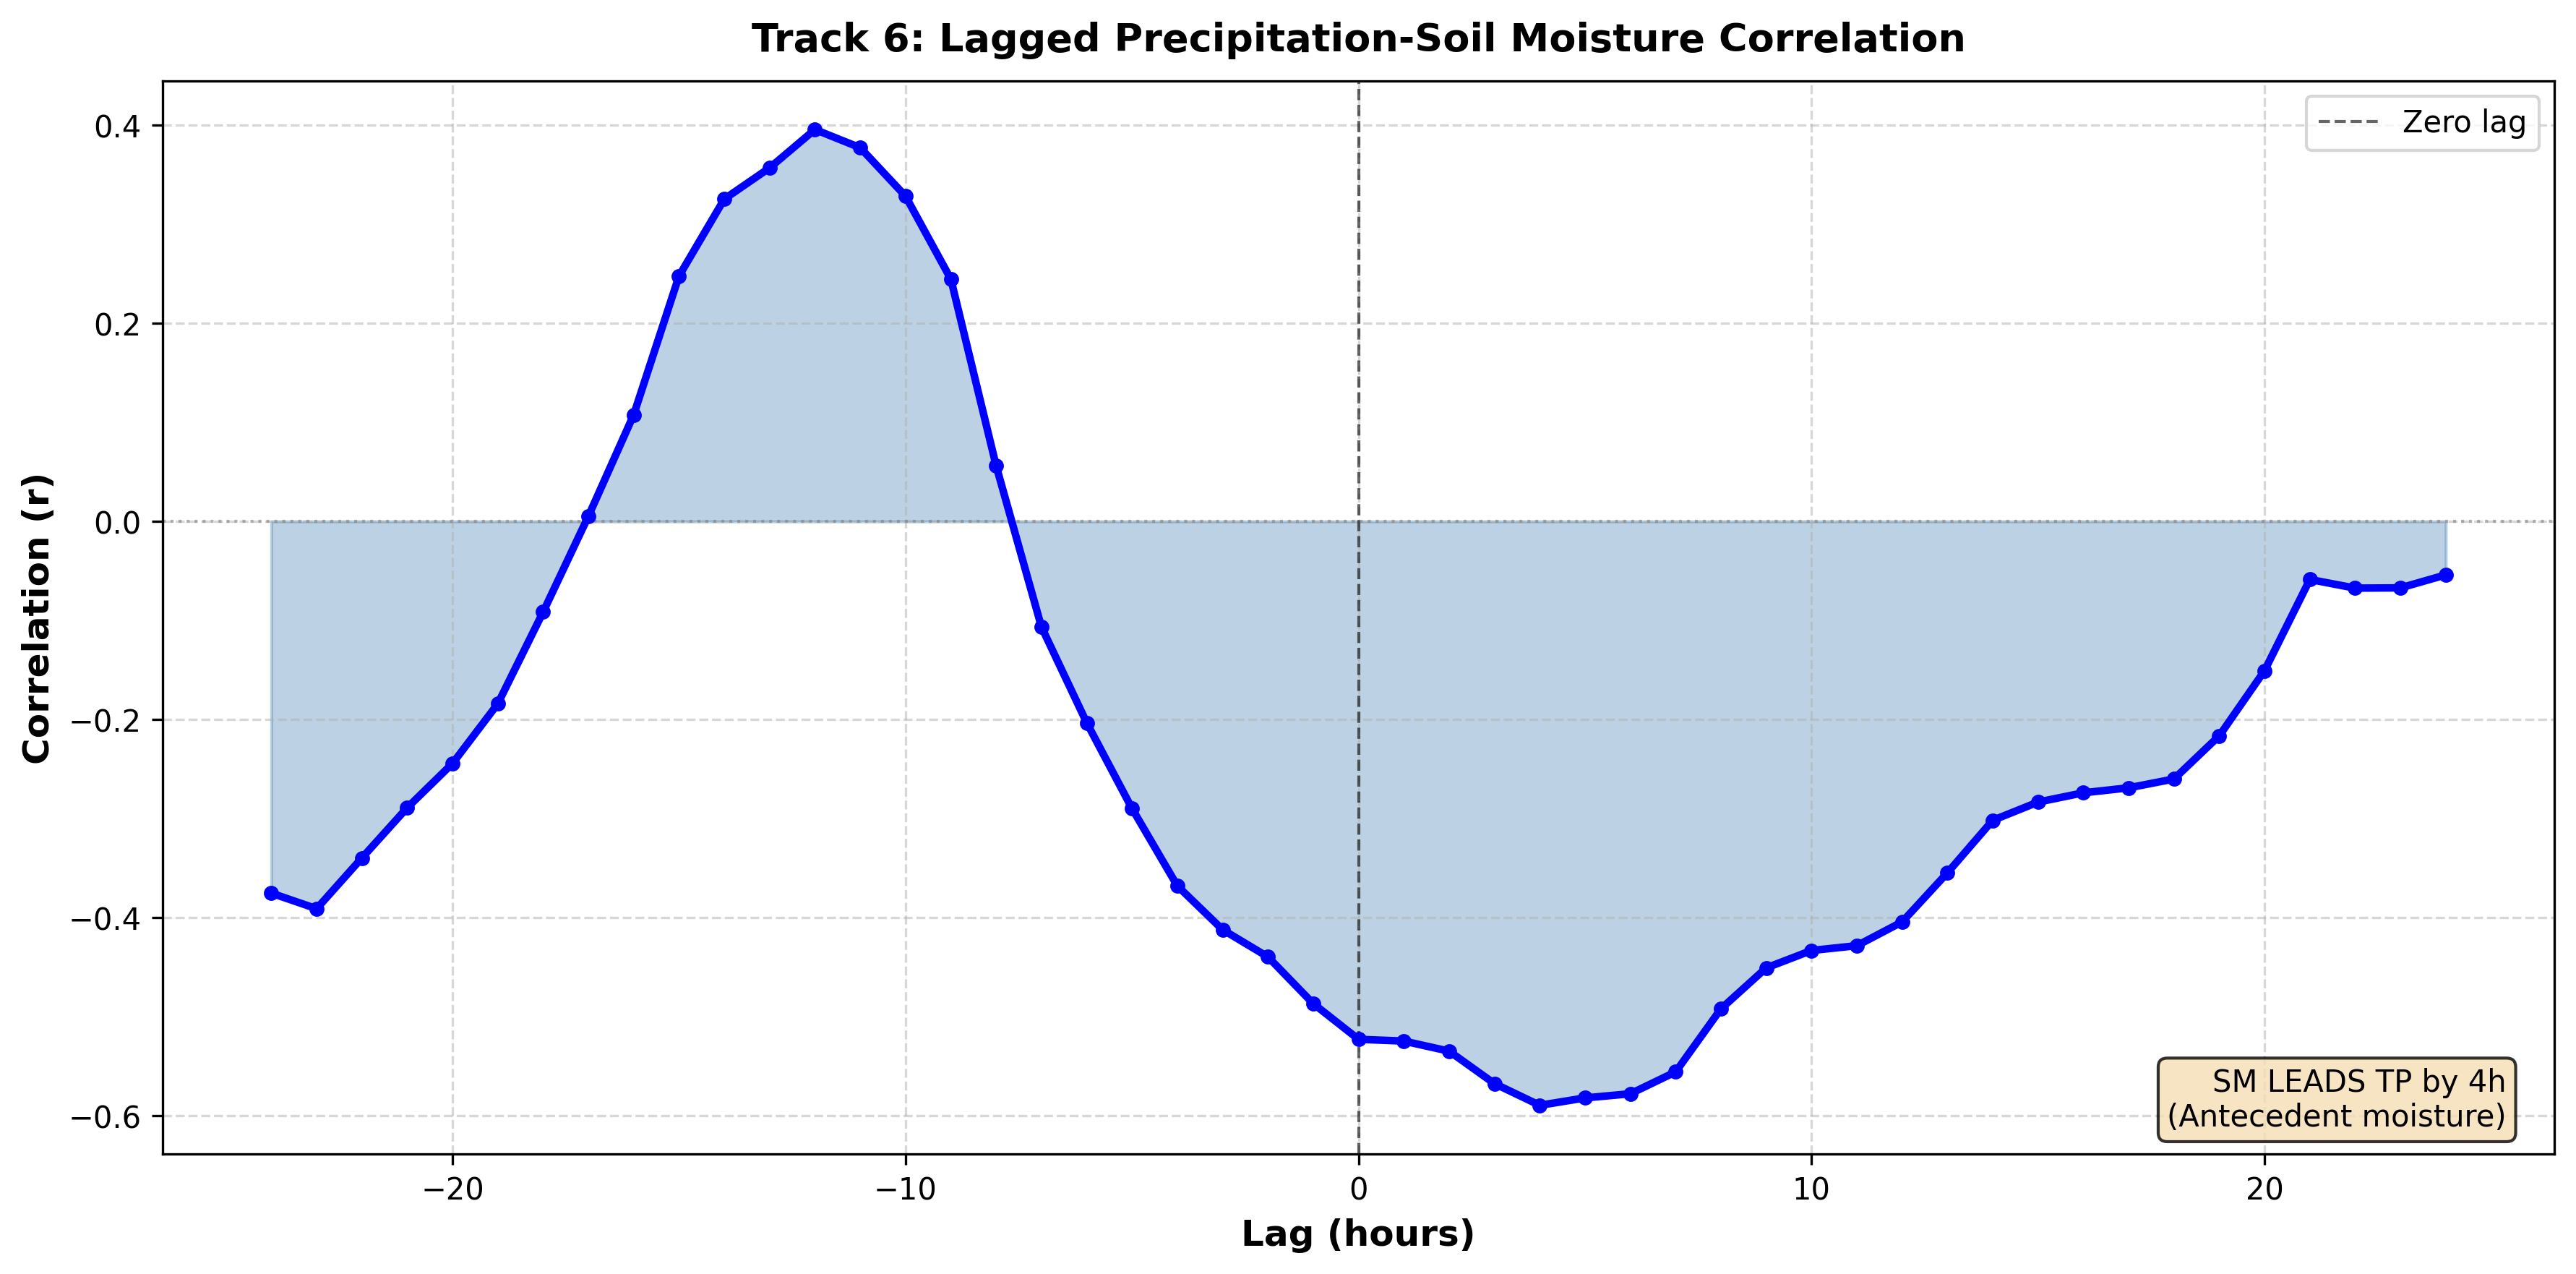
\includegraphics[width=0.8\textwidth]{../version5-with-no-ocean-masking/output/track_6/correlation_analysis/lag_correlation/track_6_lag_corr.png}
	\end{center}
\end{frame}

\begin{frame}{Track 6 Details - TP - SWVL1 Correlation}
	\begin{center}
		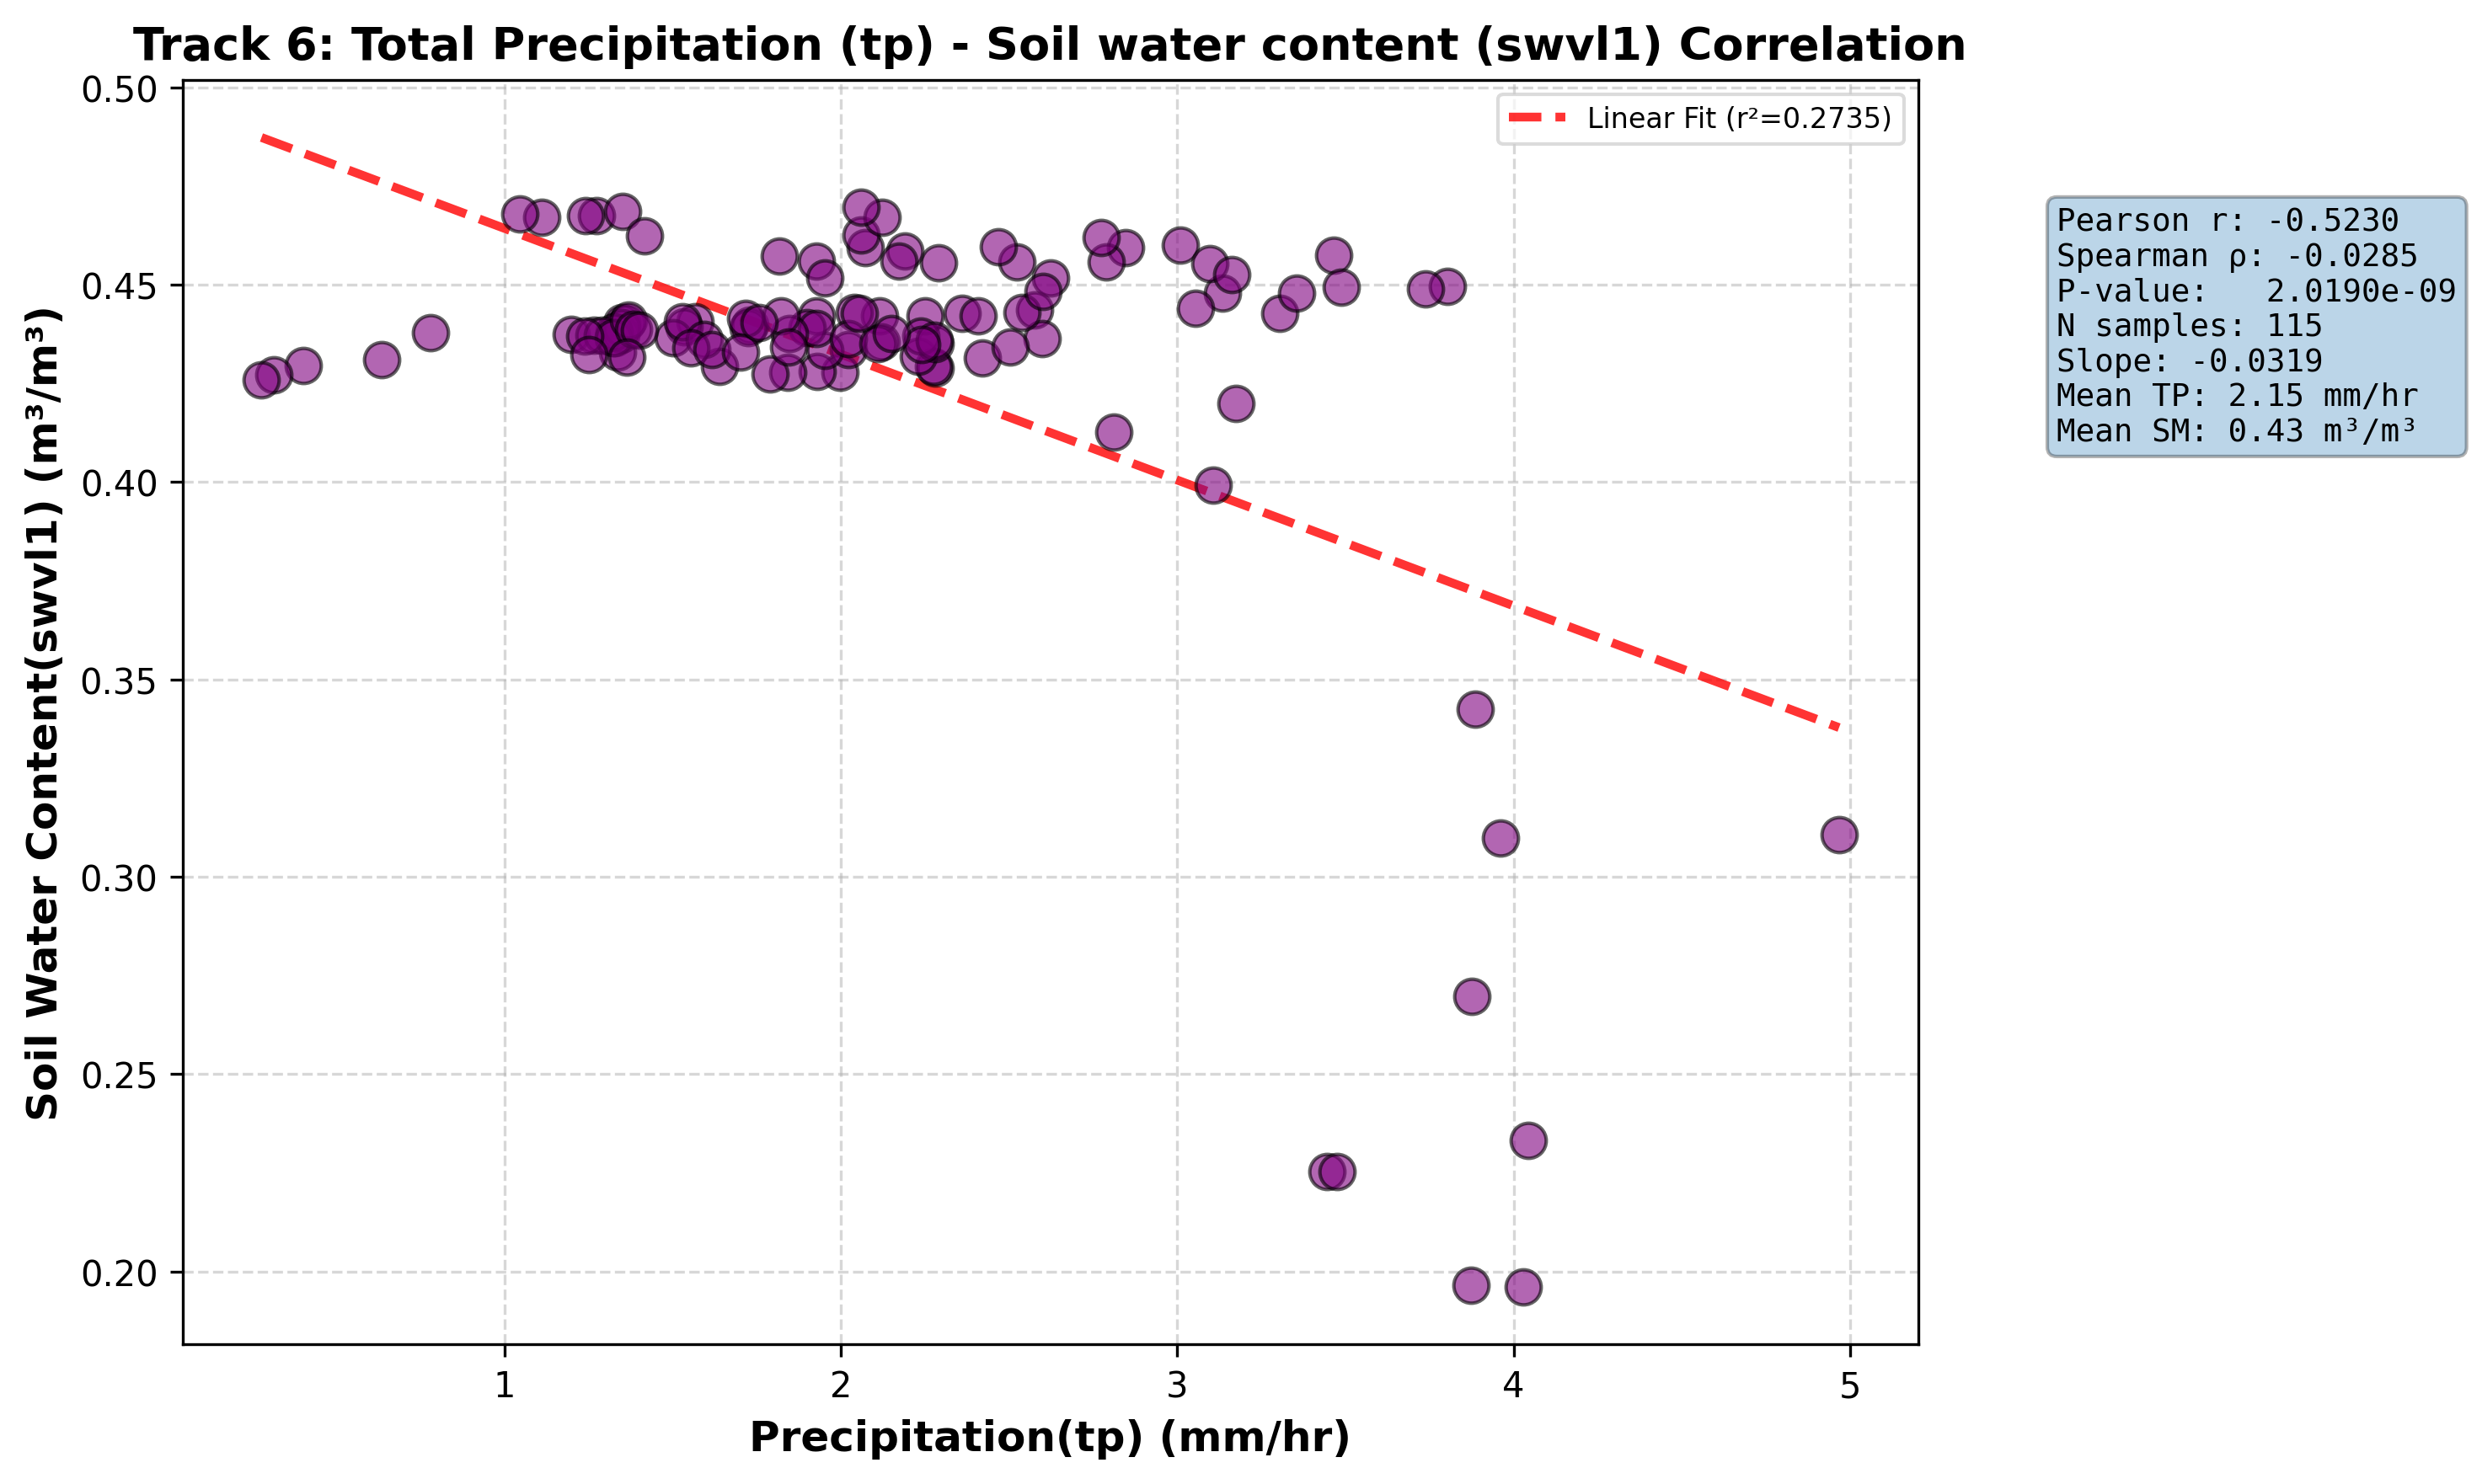
\includegraphics[width=0.7\textwidth]{../version5-with-no-ocean-masking/output/track_6/correlation_analysis/scatter_plots/track_6_scatter.png}
	\end{center}
\end{frame}

\begin{frame}{Track 6 Details - Spatial distribution of TP and SWVL1}
	\begin{center}
		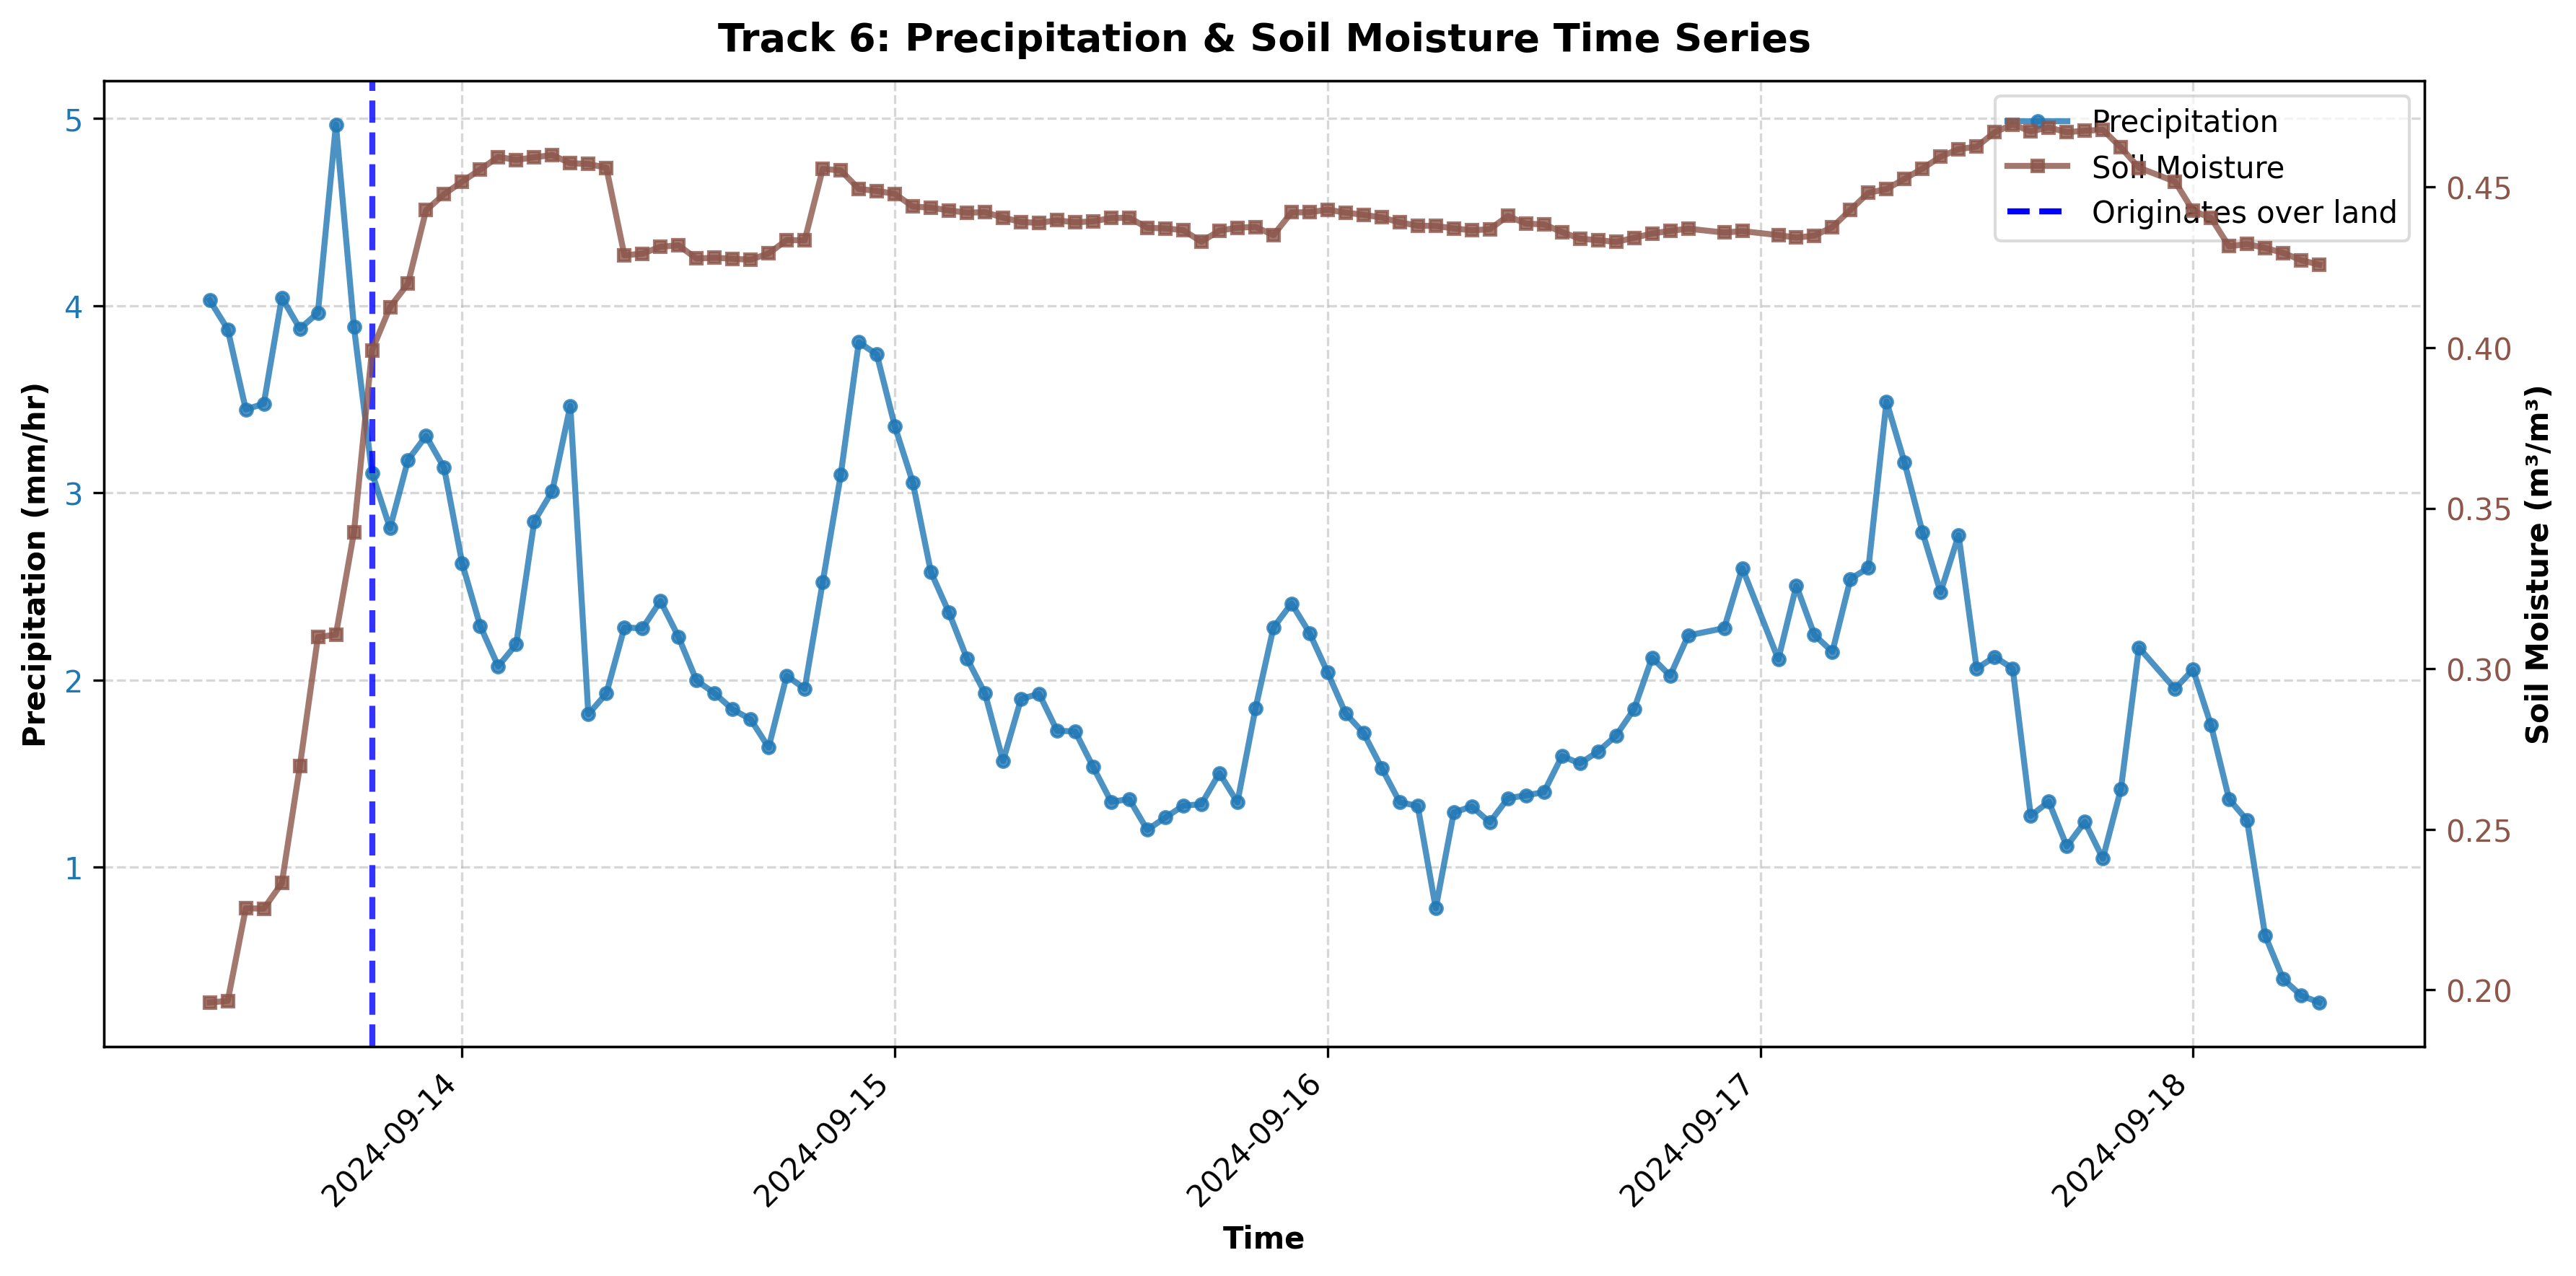
\includegraphics[width=0.7\textwidth]{../version5-with-no-ocean-masking/output/track_6/correlation_analysis/time_series/track_6_tp_sm_time_series.png}
	\end{center}
\end{frame}

% \begin{frame}{Track 6 Details - Heat fluxes transition}
% 	\begin{center}
% 		\includegraphics[width=0.8\textwidth]{../version5-with-no-ocean-masking/output/track_6/flux_analysis/track_6_analysis/track_6_heat_fluxes_trasnsition.png}
% 	\end{center}
% \end{frame}

\begin{frame}{Track 6 Details - Heat flux analysis}
	\begin{center}
		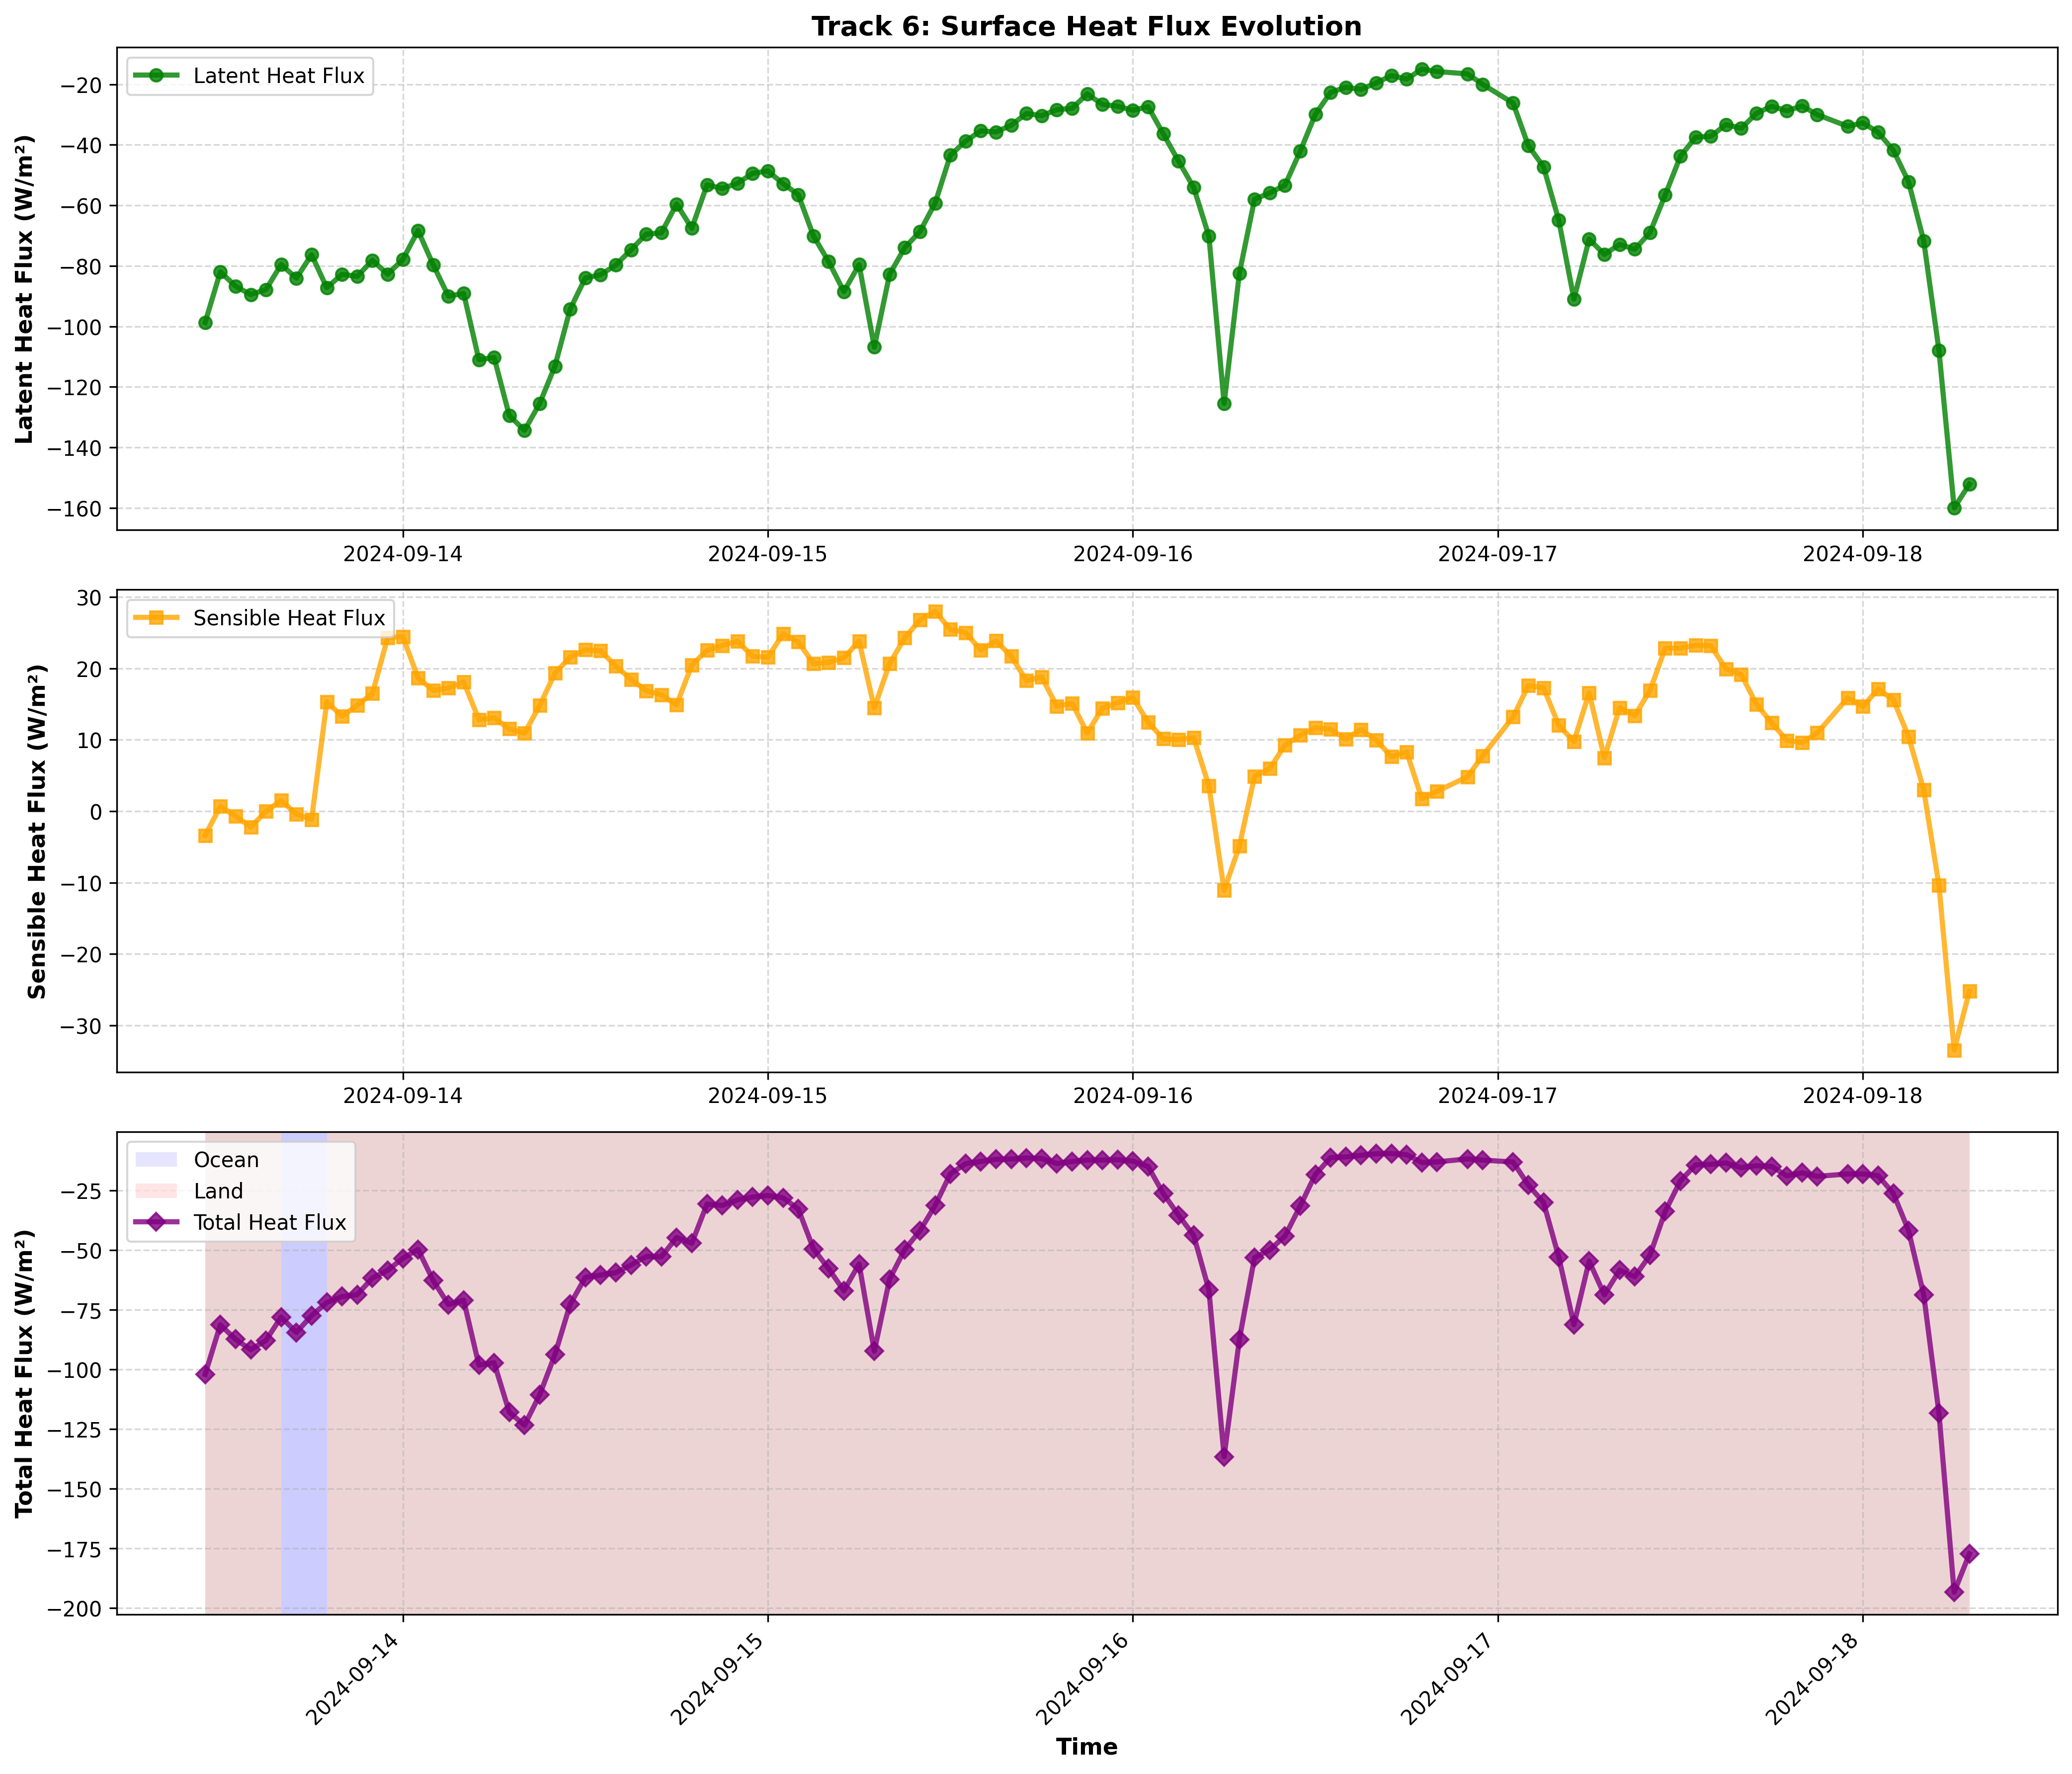
\includegraphics[width=0.6\textwidth]{../version5-with-no-ocean-masking/output/track_6/heat_flux_analysis/track_6_heat_flux_timeseries.png}
	\end{center}
\end{frame}

%%%%%%%%%%%%%%%%%%%%%%%%%%%%%%%
\section{Observations}
\begin{frame}[plain, c]
	\begin{center}
		\Huge \textcolor{blue}{\textbf{Observations}} \\
	\end{center}
\end{frame}

% Wavy / Oscillatory Patterns in Hovmöller Diagrams
\begin{frame}{Diurnal Oscillations in Azimuthal Hovm\"oller Diagrams}
	Strong periodic signals appear after land contact

	\textbf{Key variables showing clear wavy patterns:}
	\begin{itemize}
		\item Sensible heat flux: daytime peaks
		\item Latent heat flux: often inverse phase (night/early morning maxima)
		\item Soil temperature: clear diurnal cycle (2–4 K amplitude)
		\item 2 m temperature: similar to stl1 but damped
	\end{itemize}

	\vspace{0.2cm}
	\small These oscillations typically have period $\sim$24 hours and become prominent only after the MD center moves over land.

	\vspace{0.1cm}
	\begin{block}{Observation}
		Oscillatory (wavy) patterns in radial Hovm\"oller diagrams are primarily diurnal and strongly amplified once the system interacts with the land surface.
	\end{block}

	% Typical Diurnal Phase Relationships
	%Expected patterns from land–atmosphere coupling
	\vspace{0.1cm}
	\begin{block}{Why inverse LHF phase?}
		Night/early morning: lowest temperatures $\rightarrow$ highest relative humidity $\rightarrow$ lowest vapor pressure deficit $\rightarrow$ maximum evaporation when soil moisture is available.
	\end{block}
\end{frame}

% Ocean-origin vs Land-origin – Why the difference?
\begin{frame}{Why Only Land-Origin or Post-Landfall Tracks Show Strong Diurnal Waves Pattern?}
	\framesubtitle{Ocean thermal inertia vs. rapid land response}

	\footnotesize
	\begin{center}
		\begin{tabular}{p{3.15cm} | p{4.65cm} | p{4.4cm}}
			\toprule
			\textbf{Property}              & \textbf{Ocean phase}                                  & \textbf{Land phase}                           \\
			\midrule
			Diurnal signal strength        & Weak: amplitude SHF $\sim$5–20 $W/m^2$, low coherence & Strong and coherent                           \\
			Flux uniformity                & High (homogeneous sea surface)                        & Low (due to land cover, soil type, orography) \\
			Typical SHF amplitude          & $< 10$–$20$ $W/m^2$                                   & $40$–$100$ $W/m^2$ (daytime peaks)            \\
			Response time to solar forcing & Slow and damped: 3–8 h lag, amplitude heavily reduced & Fast: 1–4 h lag, amplitude close to max       \\
			% TODO: further analysis required
			% Thermal inertia                & High: weeks-scale storage in 20–100 m mixed layer     & Low: hours-scale in top 10–30 cm soil             \\
			\bottomrule
		\end{tabular}
	\end{center}

	\vspace{0.2cm}
	\footnotesize
	\begin{block}{Diagnostic signature of land contact}
		Increase in SHF daytime amplitude + emergence of $\sim$24 h periodicity in Hovm\"oller diagrams land-origin tracks and for tracks after landfall
		\begin{itemize}
			\item Daytime SHF $\rightarrow$ maintains/convective instability
			\item Nighttime LHF $\rightarrow$ sustains moisture supply overnight
		\end{itemize}
	\end{block}
\end{frame}

% Implications for MD maintenance & longevity
\begin{frame}{Implications of Diurnal Land Coupling for Monsoon Depressions}
	\framesubtitle{From diurnal waves to system maintenance}

	\footnotesize
	\textbf{Positive feedbacks over land:}
	\begin{itemize}
		\item Daytime SHF $\rightarrow$ warms boundary layer $\rightarrow$ helps maintain low-level convergence
		\item Nighttime LHF $\rightarrow$ supplies moisture to sustain convection overnight
		\item Soil moisture memory $\rightarrow$ preconditions next day's cycle
	\end{itemize}

	\vspace{0.2cm}
	\textbf{Contrast with ocean phase:}
	\begin{itemize}
		\item Nearly constant heat supply (small diurnal cycle)
		\item Moisture from large ocean reservoir
		\item Less dependence on local surface memory
	\end{itemize}
\end{frame}

\begin{frame}{Lag Correlation Analysis: TP–SWVL1}
	\footnotesize
	\textbf{Lag Interpretation:}
	\begin{itemize}
		\item \textbf{Negative Lags ($-20$ to $-1$ h):} \textit{Precipitation Leads.} TP increases \textbf{before} SWVL1 rises (Atmosphere $\rightarrow$ Land).
		\item \textbf{Positive Lags ($+1$ to $+20$ h):} \textit{Soil Moisture Leads.} SWVL1 rises \textbf{before} TP increases (Land $\rightarrow$ Atmosphere feedback).
		\item \textbf{0 Lag:} Simultaneous coupling (precipitation-evaporation syncronous feedback).
	\end{itemize}

	\vspace{0.2cm}
	\textbf{Observed Peak Correlations by Track:}
	\begin{table}
		\centering
		\small
		\begin{tabular}{p{1cm} p{1.5cm} p{2cm} p{5.5cm}}
			\toprule
			\textbf{Track} & \textbf{Peak Lag (h)} & \textbf{Sign}                                 & \textbf{Physical Interpretation}                        \\
			               &                       & \footnotesize{+ $\rightarrow$ SWVL1 leads TP} &                                                         \\
			\midrule
			1              & $-6$                  & Negative                                      & Rain $\rightarrow$ SM: Rapid infiltration (Short-lived) \\
			4              & $-12$                 & Negative                                      & Rain $\rightarrow$ SM: Infiltration delayed/Runoff      \\
			5              & $+6$                  & Positive                                      & SM $\rightarrow$ Rain: Land-surface moisture feedback   \\
			2, 3, 6        & $\sim 0$              & $\sim 0$                                      & Land-origin: Continuous coupling/steady-state           \\
			\bottomrule
		\end{tabular}
	\end{table}
\end{frame}

\begin{frame}{Diurnal Sensible Heat Flux: Land Amplifies Surface Heating}
	\footnotesize
	\begin{columns}[T]
		\column{0.3\textwidth}
		\textbf{Amplitude Comparison:}
		\begin{itemize}
			\item \textbf{Land phase:} $60.93 W/m^2$ (mean)
			\item \textbf{Ocean phase:} $13.54 W/m^2$ (mean)
		\end{itemize}

		\column{0.3\textwidth}
		\textbf{Maxima for land-phase sensible heat flux}
		\begin{itemize}
			\item Track 3: $65.3 W/m^2$
			\item Track 5: $63.7 W/m^2$
			\item Track 6: $61.5 W/m^2$
		\end{itemize}

		\column{0.3\textwidth}
		\textbf{Ocean-to-land transition:}
		\begin{itemize}
			\item Track 1: $+47.0 W/m^2$
			\item Track 4: $+46.3 W/m^2$
			\item Track 5: $+47.2 W/m^2$
		\end{itemize}
	\end{columns}

	\vspace{0.2cm}
	\begin{block}{Physical Meaning}
		\begin{itemize}
			\item Land surfaces create strong diurnal heating cycles
			\item Ocean thermal inertia damps diurnal variations
			\item Larger amplitude = stronger daytime convection
		\end{itemize}
	\end{block}
\end{frame}

\begin{frame}{Soil Water Capacity: Enabling but Not Guaranteeing Longevity}
	\textbf{Moisture Capacity Index = Normalized soil moisture (0=dry, 1=saturated)}
	\vspace{0.3cm}

	\footnotesize
	\begin{columns}[T]
		\column{0.5\textwidth}
		\textbf{High moisture holding capacity:}
		\begin{itemize}
			\item Track 6: 0.768 (plains/clay soil)
			\item Track 3: 0.758 (plains/clay soil)
			\item Track 2: 0.708 (plains/clay soil)
		\end{itemize}

		\column{0.5\textwidth}
		\textbf{Low moisture holding capacity:}
		\begin{itemize}
			\item Track 1: 0.242 (coastal/sandy soil)
			\item Track 5: 0.433 (mixed soil, first sandy then clay on furthur inland)
			\item Track 4: 0.380 (coastal/sandy soil)
		\end{itemize}
	\end{columns}

	\vspace{0.2cm}
	\begin{block}{Key Finding}
		High capacity necessary but not sufficient for longevity
		\begin{itemize}
			\item Track 1,4: Low capacity $\rightarrow$ Short duration
			\item Track 5: Moderate capacity + Other factors $\rightrightarrows$ Long duration
			\item Tracks 2,3,6: High capacity + Strong coupling $\rightarrow$ Long duration
		\end{itemize}
	\end{block}
\end{frame}

\begin{frame}{Feedback Strength Index (FSI): Measuring TP-SWVL1 Coupling Efficiency}
	\textbf{FSI = Correlation Strength $\times$ Soil Capacity}
	\begin{itemize}
		\item High FSI: Efficient rainfall-soil moisture feedback
		\item Low FSI: Inefficient or negative feedback
	\end{itemize}

	\begin{columns}[T]
		\column{0.5\textwidth}
		\textbf{Key Findings:}
		\begin{itemize}
			\item \textbf{Strongest coupling:} Track 3 ($FSI = 0.604$)
			\item \textbf{Weakest coupling:} Track 1 ($FSI = 0.063$)
			\item \textbf{All tracks show statistically significant coupling} ($p<0.05$)
			\item Mean $FSI = 0.298 \pm 0.213$
		\end{itemize}

		\column{0.5\textwidth}
		\textbf{Track-wise FSI values:}
		\begin{tabular}{lll}
			\toprule
			Track & FSI   & Correlation \\
			\midrule
			1     & 0.063 & -0.263      \\
			2     & 0.423 & 0.598       \\
			3     & 0.604 & 0.797       \\
			4     & 0.088 & -0.231      \\
			5     & 0.210 & 0.485       \\
			6     & 0.402 & -0.523      \\
			\bottomrule
		\end{tabular}
	\end{columns}

	\vspace{0.3cm}
	\begin{block}{Interpretation}
		\begin{itemize}
			\item \textbf{Positive correlation tracks (2,3,5):} Soil moisture $\rightarrow$ Rainfall feedback
			\item \textbf{Negative correlation tracks (1,4,6):} Rainfall $\rightarrow$ Soil moisture infiltration
			\item Higher FSI indicates more efficient land-atmosphere energy exchange
		\end{itemize}
	\end{block}
\end{frame}

\begin{frame}{Coupling Efficiency}
	\textbf{Feedback Strength Index (FSI) = Correlation Strength $\times$ Soil Capacity}


	\textbf{Coupling Efficiency = FSI $\times$ Diurnal Amplitude $\times$ Duration Factor}
	\vspace{0.3cm}

	\footnotesize
	\begin{columns}[T]
		\column{0.3\textwidth}
		\textbf{Highest efficiency:}
		\begin{itemize}
			\item Track 2: 0.127
			\item Track 3: 0.114
			\item Track 6: 0.113
		\end{itemize}

		\column{0.3\textwidth}
		\textbf{Lowest efficiency:}
		\begin{itemize}
			\item Track 5: 0.033 (despite long duration)
			\item Track 4: 0.034
			\item Track 1: 0.023
		\end{itemize}

		\column{0.3\textwidth}
		\textbf{Patterns observed:}
		\begin{itemize}
			\item \textbf{Land-origin tracks} generally higher coupling efficiency
			\item \textbf{Long-lived tracks} maintain moderate-high efficiency
			\item \textbf{Ocean-origin short tracks} lowest efficiency
		\end{itemize}
	\end{columns}

	\vspace{0.2cm}
	\begin{block}{Key Insight}
		Track 5 (165h) has low coupling efficiency (0.033) despite long duration - suggests other mechanisms sustaining it
	\end{block}
\end{frame}
%%%%%%%%%%%%%%%%%%%%%%%%%%%%%%%

\section{Proposed Hypotheses}
\begin{frame}[c]
	\begin{center}
		\Huge \textcolor{blue}{\textbf{Proposed Hypotheses}} \\
	\end{center}
\end{frame}

\begin{frame}{Hypothesis 1: The Moisture-Recycling Efficiency (TP-SWVL1 Feedback and Lags) [1/2]}
	Statement : The longevity of an MD over land depends on the synchrony of the Precipitation-Soil Moisture-Flux feedback loop. Long-lived monsoon depressions ($\ge 96$ hours) maintain higher magnitude surface energy exchange over land through sustained mesoscale organization and continuous moisture recycling. Short-lived systems ($< 96$ hours) undergo rapid decay post-landfall as internal dynamics collapse in response to land-surface friction and moisture depletion.

	\vspace{0.05cm}
	TP-SWVL1 feedback is temporally lagged ($-12$-$+6$ hours) indicating both rain-driven and soil-driven regions.

	The feedback loop operates as: (Rainfall) $\rightarrow$ (Infiltration lag 6-12h) $\rightarrow$ (Elevated SM) $\rightarrow$ (Sustained LHF) $\rightarrow$ (MD continuation). Short-lived MDs (Tracks 1, 4) show broken lags ($>12h$) or persistent negative correlation, indicating runoff-dominated response on sandy soil.
\end{frame}

\begin{frame}{Hypothesis 1: The Moisture-Recycling Efficiency (TP-SWVL1 Feedback and Lags) [2/2]}
	Evidence:
	\begin{itemize}
		\item All 6 tracks showed significant $(p<0.05)$ correlation between TP and SM, but mean correlation magnitude was low $(0.144)$.
		      \begin{itemize}
			      \item \textbf{Track 1 (75h, ocean-origin):} ASM increased from $0.0367$ (24h before) to $0.1098$ (6h before), jumping to $0.2253$ post-landfall (6$\times$ increase). Negative TP-SWVL1 correlation $(r=-0.252)$ suggests rapid but runoff-dominated response.
			      \item \textbf{Track 4 (75h, ocean-origin):} ASM rose from $0.0713$ (24h before) to $0.1370$ (6h before), peaking at $0.3275$ post-landfall (4.6$\times$ increase). Strong negative correlation $(r=-0.526)$.
			      \item \textbf{Track 5 (165h, ocean-origin):} ASM climbed from $0.0281$ (24h before) to $0.0979$ (6h before), reaching $0.2807$ post-landfall (10$\times$ increase). Strong positive correlation $(r=+0.684)$ despite lowest pre-landfall moisture.
			      \item \textbf{Track 6 (117h, land-origin):} $\text{ASM}_{24h} = 0.1966\ \text{m}^3/\text{m}^3$ (highest among all tracks). Positive correlation observed.
			      \item \textbf{Tracks 2 \& 3 (land-origin):} No ASM progression data (no discrete landfall). Weak positive TP-SWVL1 feedback sustained over clay plains.
		      \end{itemize}
	\end{itemize}

	% TODO:
	% - Lag at max correlation for each track.
	% - Strength of correlation at that lag.

	\vspace{0.05cm}
	Key Predictions :
	\begin{itemize}
		\item Longevity is higher when the "recharge" from rainfall immediately offsets the "depletion" from surface heat fluxes.
		\item Long-lived MDs: Lower decay rate of latent flux over land; sustained sensible heating; longer precipitation duration
		\item Short-lived MDs: Rapid latent flux collapse post-landfall; weak sensible signal; shorter
	\end{itemize}
\end{frame}

\begin{frame}{Hypothesis 2: Landfall Represents Energy Budget Transition [1/2]}
	Statement: Ocean-to-land transition during MD passage produces a measurable and statistically significant reduction in surface evaporative cooling (latent heat flux magnitude), reflecting the constraint of water/moisture availability over land. This energy budget shift manifests as increased sensible heating and lower total surface heat uptake over land compared to ocean phases.
\end{frame}

\begin{frame}{Hypothesis 2: Landfall Represents Energy Budget Transition [2/2]}
	\vspace{0.05cm}
	Evidence:
	\begin{itemize}
		\item Ocean-origin, short-lived MDs (Tracks 1, 4):
		      \begin{itemize}
			      \item Large reduction in upward flux magnitude ($\Delta HF \approx +40$ to $+80 W/m^2$)
			      \item Rapid LHF collapse post-landfall (surface moisture supply from ocean cut off)
			            % \item LHF collapse: ocean evaporation ceases faster than soil moisture can sustain
			      \item Total surface energy flux moves significantly closer to zero
			      \item SHF compensation insufficient leads to rapid dissipation
			      \item Result: Rapid boundary layer destabilization -> dissipation within 72h
		      \end{itemize}

		\item Ocean-origin, long-lived MD (Track 5):
		      \begin{itemize}
			      \item Sustained high-magnitude fluxes ($\Delta HF$ is smaller, e.g., $< +20 W/m^2$)
			      \item Sustained LHF facilitated by high antecedent soil moisture
			      \item Soil moisture feedback stabilizes energy budget
			      \item Surface continues to provide energy levels comparable to ocean phases
			      \item Result: Extended energy balance allows survival >150h
		      \end{itemize}
		\item Land-origin MDs (Tracks 2, 3, 6):
		      \begin{itemize}
			      \item  No discrete landfall transition (already terrestrial)
			      \item  Energy source: antecedent soil moisture rather than coastal evaporation
		      \end{itemize}
	\end{itemize}

	% \vspace{0.05cm}
	% Key Predictions :
	% \begin{itemize}
	% 	\item Observed landfall flux transition: $+68.8 W/m^2$ change (before: $-153.6$ -> after: $-84.8 W/m^2$)
	% 	\item Ocean phase: unlimited moisture for evaporation -> strong latent cooling signal
	% 	\item Land phase: limited soil moisture availability -> reduced latent heat flux, increased sensible heat flux
	% \end{itemize}
\end{frame}

% \begin{frame}{Nonlinear Soil Moisture-Precipitation Dynamics}
% 	Statement: The relationship between monsoon precipitation and soil moisture is fundamentally nonlinear and time-lagged rather than instantaneous. A 6-12 hour lag exists between maximum precipitation intensity and peak soil moisture response, and the sensitivity of SWVL1 to TP changes is modulated by baseline antecedent saturation (drier soils show higher sensitivity; saturated soils show saturation-plateau behavior).
%
% 	\vspace{0.05cm}
% 	Evidence:
% 	\begin{itemize}
% 		\item Weak instantaneous correlation (r = 0.144) may reflect temporal mismatch
% 		\item Peak soil moisture response lags peak infiltration by soil-profile-depth/infiltration-rate
% 		\item Saturation plateau effect: saturated soils cannot increase SWVL1 further regardless of TP increase
% 	\end{itemize}
%
% \end{frame}

\begin{frame}{Hypothesis 3: Soil Type Modulation}
	Statement : Soil type determines the efficiency of TP $\rightarrow$ SWVL$_1$ $\rightarrow$ HF energy transfer pathway. Clay soils enable longer feedback loops than sandy soils.

	\vspace{0.05cm}
	Key Predictions :
	\begin{itemize}
		\item Indo-Gangetic tracks (clay) $\Rightarrow$ positive TP-SWVL$_1$ + long duration
		\item Coastal tracks (sandy) $\Rightarrow$ negative TP-SWVL$_1$ + short duration
	\end{itemize}

	\vspace{0.05cm}
	Evidence :
	\begin{center}
		\begin{tabular}{llll}
			\textbf{Region} & \textbf{Soil Type} & \textbf{Tracks} & \textbf{Avg Duration} \\
			\midrule
			Coastal         & Sandy              & 1, 4            & 73h                   \\
			Plains          & Clay               & 2, 3, 5, 6      & 135h                  \\
		\end{tabular}
	\end{center}

	% TODO:explicitly map soil type along each track using a soil dataset (e.g., FAO Soil Grids) to confirm clay vs. sandy regions.

	\vspace{0.05cm}
	\begin{block}{Confirmes}
		Clear regional pattern: clay soils over Indo-Gangetic plain support longer duration.
	\end{block}
\end{frame}

% \begin{frame}{Hypothesis 4 (Revised): Two-Tier Mechanism}
% 	Revised Statement : Actual duration is determined by pre-landfall soil moisture (ASM$_{24h}$) and atmospheric TP-SWVL$_1$ coupling strength.
%
% 	\vspace{0.05cm}
% 	\begin{block}{Integrated Mechanism}
% 		\begin{itemize}
% 			\item \textbf{Tier 1 (Necessary)}: Soil Type
% 			      \begin{itemize}
% 				      \item Clay soils: capacity for 120-180h duration
% 				      \item Sandy soils: capacity for 50-100h duration
% 			      \end{itemize}
% 			\item \textbf{Tier 2 (Sufficient)}: Pre-landfall ASM + TP-SWVL$_1$ coupling
% 			      \begin{itemize}
% 				      \item High ASM + positive feedback $\Rightarrow$ maximum duration and longer longevity
% 				      \item Low ASM + negative feedback $\Rightarrow$ minimum duration and shorter longevity
% 			      \end{itemize}
% 		\end{itemize}
% 	\end{block}
%
% 	\vspace{0.05cm}
% 	\begin{block}{Example Trajectories}
% 		\begin{itemize}
% 			\item Track 5 (coastal sand$\rightarrow$ plains clay): 165h (ocean$\rightarrow$land progression)
% 			\item Track 1 (coastal sand): 71h (weak feedback loop)
% 			\item Track 3 (plains clay): 154h (strong feedback sustained)
% 		\end{itemize}
% 	\end{block}
% \end{frame}

\begin{frame}{Hypothesis 4 : Soil Moisture Provides Infiltration Capacity, but not necessary conditions [1/2]}
	% Statement : Pre-landfall soil moisture ($ASM_{24h}$) acts as a Necessary but Not Sufficient condition.
	Statement : Pre-landfall soil moisture ($ASM$) enables infiltration, but longevity depends on soil type and TP-SWVL1 coupling strength.

	\vspace{0.05cm}
	The antecedent soil moisture condition (24 hours pre-landfall) is a stronger predictor of monsoon depression behavior and energy budget characteristics than instantaneous precipitation during passage. Drier antecedent soils enhance infiltration capacity; wet antecedent conditions promote surface runoff and rapid downslope transport.

	\vspace{0.05cm}
	Antecedent soil moisture ($ASM_{24h}$) is a necessary background condition for infiltration but does NOT directly predict MD longevity. Ocean-origin tracks have pre-landfall ASM ranging from $0.028$–$0.071 m^3/m^3$, yet durations range from $75$–$165h$.
\end{frame}

\begin{frame}{Hypothesis 4 : Soil Moisture Provides Infiltration Capacity, but not necessary conditions [2/2]}
	Evidence:
	\begin{itemize}
		\item No correlation between $ASM_{24h}$ and duration
		\item Lowest ASM (Track 5: 0.028) $\rightarrow$ Longest duration (165h)
		\item Highest ASM (Track 4: 0.071) $\rightarrow$ Short duration (75h)
		\item All tracks show 4-10 ASM increase by landfall regardless of final duration
	\end{itemize}

	\vspace{0.05cm}
	Key Predictions :
	\begin{itemize}
		\item Tracks 1, 4, and 5 (ocean-originated) have valid ASM ($>0.05 m^3/m^3$) values. This supports the "moist environment" over land 24 hours before lanfall.
		      \begin{itemize}
			      \item Track 1: ASM (24h) = $0.037 m^3/m^3$
			      \item Track 4: ASM (24h) = $0.071 m^3/m^3$
			      \item Track 5: ASM (24h) = $0.028 m^3/m^3$
		      \end{itemize}
	\end{itemize}
\end{frame}

\section{Conclusions}
\begin{frame}[plain, c]
	\begin{center}
		\Huge \textcolor{blue}{\textbf{Conclusions}} \\
	\end{center}
\end{frame}

\begin{frame}{Heat Flux Transition: Ocean vs. Land}
	\begin{columns}[T]
		\column{0.5\textwidth}
		\textbf{Ocean Phase (Before Landfall):}
		\begin{itemize}
			\item High Latent HF (evaporation)
			\item Low Sensible HF
			\item Total HF dominates
			\item MD strengthens
		\end{itemize}

		\column{0.5\textwidth}
		\textbf{Land Phase (After Landfall):}
		\begin{itemize}
			\item LHF drops sharply
			\item SHF increases (soil heating)
			\item Total HF decreases
			\item Yet 67\% MDs survive
		\end{itemize}
	\end{columns}

	\vspace{0.3cm}
	\textbf{The Paradox:} Energy flux \textbf{decreases} at landfall, yet most MDs persist.

	\textbf{Explanation:} Soil moisture and pre-wetted land act as thermal battery.
\end{frame}

\begin{frame}{MD Classification Based on Coupling Characteristics}
	\begin{columns}[T]
		\column{0.33\textwidth}
		\textbf{Strongly Coupled}
		\begin{itemize}
			\item Tracks: 2, 3, 6
			\item FSI: 0.40-0.60
			\item Efficiency: 0.11-0.13
			\item Duration: 105-154h
			\item Origin: Land (2,3,6)
		\end{itemize}

		\column{0.33\textwidth}
		\textbf{Moderately Coupled}
		\begin{itemize}
			\item Track: 5
			\item FSI: 0.21
			\item Efficiency: 0.033
			\item Duration: 165h
			\item Origin: Ocean
			\item Anomaly: Long despite moderate coupling
		\end{itemize}

		\column{0.33\textwidth}
		\textbf{Weakly Coupled}
		\begin{itemize}
			\item Tracks: 1, 4
			\item FSI: 0.06-0.09
			\item Efficiency: 0.02-0.03
			\item Duration: 75h
			\item Origin: Ocean
		\end{itemize}
	\end{columns}

	\vspace{0.3cm}
	\begin{block}{Implication for Forecasting}
		\begin{itemize}
			\item Coupling metrics provide early indicators of longevity
			\item FSI + Diurnal Amplitude > threshold predicts long-lived MDs
			\item Track 5 suggests other factors (moisture advection?) important
		\end{itemize}
	\end{block}
\end{frame}

% % % \begin{frame}[allowframebreaks]{Conclusions}
% % % 	% TODO:
% % % 	\begin{enumerate}
% % % 		\item For tracks 1, 4, 5 (which transition from ocean to over land) there is sharp increase in SHF and total heat flux as MD landfall indicating MD is now interacting with a heated land surface rather than ocean (thermal reservoir).
% % % 		\item LHF decrease as MD moves from over the Bay of Bengal to inland, the MD has lost its primary fuel source (moisture evaporation).
% % % 		\item In flux Analysis scatter plot a cluster in the top right, indicating of the Brown Ocean Effect -> the system is extracting massive energy from the wet ground. Analysis: Moisture-Flux Coupling: The high correlation between SWVL1 and Total\_HF (r = 0.252 for track 1, 0.526 for track 4 and 0.684 for track 5) proves that the heat flux received is directly powered by the moisture in the soil.
% % % 		\item Core Maintenance: Because the Latent Heat Flux (LHF) remains robust over land, the MD maintains its "warm core" and low-pressure center, leading to increased longevity.
% % % 		\item Latent Heat Flux (LHF): (for track 1) The data shows LHF changing from -133.99 (ocean) to -99.57 (land). Note: negative indicate upward flux from surface to atmosphere. Analysis: LHF remains significantly high (near -100 W/m²) after landfall is the reason for the MD's sustainability.
% % % 		\item Scatter plot: correlation between tp vs swvl1 is negative for short track and with landfall (1, 4) while for long track (5) correlation is positive. -> This implies (for track 1 and 4), indicates a temporal lag. Heavy precipitation occurs first, followed by a rise in soil moisture. The MD's own precipitation "recharges" the soil. This creates a self-sustaining mechanism: MD produces Rain > Rain increases SM > High SM increases Heat Flux > Heat Flux fuels the MD.
% % % 		\item ASM\_24h (Antecedent Soil Moisture) of 0.0193 m\textsuperscript{3}/m\textsuperscript{3} (for track 1) and 0.0551 m\textsuperscript{3}/m\textsuperscript{3} (for track 4) lies in the spatial "pre-conditioning." High soil moisture reduces the temperature gradient between the ocean and land. if Track sustained its intensity over land, we can argue that this antecedent moisture prevented the "thermal desert" effect (where dry land usually kills a storm). This supports the Brown Ocean Effect hypothesis-the land is acting like a continuation of the sea.
% % % 		\item overall conclusion Heat Flux is the mediator. Soil moisture is the "reservoir," but the Heat Flux is the "pump" that transfers that energy into the MD's core, allowing it to maintain its cyclonic structure despite surface friction.
% % % 		\item Soil Type Sensitivity: Clay soils (higher water-holding capacity) sustain MDs longer than sandy soils
% % % 		      \begin{itemize}
% % % 			      \item Track 5 propagate over IndoGangetic plains which is clayey soil (hold more moisture) than coastal region for track 1 and 4. Therefore expected longer duration of track 5 ($\sim$7 days) than track 1 ($\sim$ 3days) and 4 ($\sim$3 days)
% % % 		      \end{itemize}
% % % 	\end{enumerate}
% % \end{frame}
% %
% % \begin{frame}{Primary Conclusions}
% % 	\large
% % 	\textbf{Monsoon Depression inland longevity is controlled by a two-level mechanism:}
% %
% % 	\normalsize
% % 	\vspace{0.2cm}
% % 	(1) \textbf{Soil type} determines potential for long-duration survival through enhanced water retention and thermal capacity. \n
% % 	(2) \textbf{Pre-landfall soil moisture + TP-SWVL$_1$ coupling} determines actual duration within soil-type limits.
% %
% % 	\vspace{0.2cm}
% % 	\begin{block}{Why Energy Decreases Yet MD Survives}
% % 		\begin{itemize}
% % 			\item Atmospheric HF decreases at landfall (observed)
% % 			\item But \textbf{soil acts as latent heat reservoir} (hypothesis)
% % 			\item Pre-landfall soil moisture stores thermal energy
% % 			\item MD survives by using heat flux from soil, not atmospheric heat flux
% % 		\end{itemize}
% % 	\end{block}
% % \end{frame}
% %
% % \begin{frame}{Implications for Monsoon Forecasting}
% % 	\begin{block}{Predictability Framework}
% % 		For improved MD longevity forecasts:
% % 		\begin{enumerate}
% % 			\item Map pre-landfall soil moisture (ASM$_{24h}$) at hourly resolution
% % 			\item Classify soil type at impact region
% % 			\item Predict TP-SWVL$_1$ coupling strength (via atmospheric indices)
% % 			\item Apply two-tier model to estimate duration
% % 		\end{enumerate}
% % 	\end{block}
% %
% % 	\vspace{0.05cm}
% % 	\begin{block}{Expected Forecast Skill}
% % 		\begin{itemize}
% % 			\item Soil type classification: 85\% confidence
% % 			\item ASM threshold testing: Needs 2025 validation
% % 			\item TP-SWVL$_1$ synchrony: Requires temporal lag analysis
% % 			\item Combined model: Potential 70-80\% skill for 96h duration forecast
% % 		\end{itemize}
% % 	\end{block}
% %
% % 	\vspace{0.05cm}
% % 	\begin{block}{Climate Change Implications}
% % 		\begin{itemize}
% % 			\item If soil drying trend persists: shorter-lived MDs expected
% % 			\item If monsoon intensity increases: TP-SWVL$_1$ feedback strengthens
% % 			\item Inland flood risk depends on BOTH factors, not just rainfall
% % 		\end{itemize}
% % 	\end{block}
% % \end{frame}
%
% % \begin{frame}{Knowledge Gaps \& Future Research}
% % 	\begin{block}{Critical Gaps}
% % 		\begin{enumerate}
% % 			\item Quantify ASM$_{24h}$ values and validate threshold hypothesis
% % 			\item Perform lagged-correlation analysis (TP at lags 0, 6h, 12h, 24h)
% % 			\item Match track coordinates to real soil property datasets
% % 			\item Decompose HF into ocean-phase vs. land-phase evolution
% % 			\item Test feedback synchrony hypothesis (temporal lags)
% % 		\end{enumerate}
% % 	\end{block}
% %
% % 	\vspace{0.05cm}
% % 	\begin{block}{Extended Questions}
% % 		\begin{enumerate}
% % 			\item Do stronger MDs generate more effective feedback loops?
% % 			\item What is the relationship between MD intensity and TP-SWVL$_1$ coupling?
% % 			\item How does orography modulate soil moisture effectiveness?
% % 		\end{enumerate}
% % 	\end{block}
% %
% % 	\vspace{0.05cm}
% % 	\begin{block}{Validation Strategy}
% % 		Apply this framework to 2025 monsoon season:
% % 		\begin{itemize}
% % 			\item Forecast MD duration 24-48h in advance
% % 			\item Compare to IMD observations
% % 			\item Refine ASM threshold and feedback parameters
% % 			\item Extend to other monsoon regions (WNP, Atlantic)
% % 		\end{itemize}
% % 	\end{block}
% % \end{frame}
% %
% % \begin{frame}{Final Summary}
% % 	\begin{center}
% % 		\Large
% % 		\textbf{Why Some Monsoon Depressions Die Over Land While Others Thrive?}
% % 		\normalsize
% % 	\end{center}
% %
% % 	\vspace{0.3cm}
% % 	\textbf{Answer: Soil type and Pre-landfall condition matters as much as the atmosphere (Heat fluxes)}
% %
% % 	\vspace{0.3cm}
% % 	\begin{itemize}
% % 		\item Soil type sets the \textbf{capacity}.
% % 		\item Soil moisture sets the \textbf{fuel}.
% % 		\item Precipitation-soil feedback sets the \textbf{efficiency} also for longevity.
% % 	\end{itemize}
% % \end{frame}

\end{document}
